% Options for packages loaded elsewhere
\PassOptionsToPackage{unicode}{hyperref}
\PassOptionsToPackage{hyphens}{url}
%
\documentclass[
  11pt,
]{env/yjiao}
\usepackage{lmodern}
\usepackage{setspace}
\usepackage{amssymb,amsmath}
\usepackage{ifxetex,ifluatex}
\ifnum 0\ifxetex 1\fi\ifluatex 1\fi=0 % if pdftex
  \usepackage[T1]{fontenc}
  \usepackage[utf8]{inputenc}
  \usepackage{textcomp} % provide euro and other symbols
\else % if luatex or xetex
  \usepackage{unicode-math}
  \defaultfontfeatures{Scale=MatchLowercase}
  \defaultfontfeatures[\rmfamily]{Ligatures=TeX,Scale=1}
\fi
% Use upquote if available, for straight quotes in verbatim environments
\IfFileExists{upquote.sty}{\usepackage{upquote}}{}
\IfFileExists{microtype.sty}{% use microtype if available
  \usepackage[]{microtype}
  \UseMicrotypeSet[protrusion]{basicmath} % disable protrusion for tt fonts
}{}
\makeatletter
\@ifundefined{KOMAClassName}{% if non-KOMA class
  \IfFileExists{parskip.sty}{%
    \usepackage{parskip}
  }{% else
    \setlength{\parindent}{0pt}
    \setlength{\parskip}{6pt plus 2pt minus 1pt}}
}{% if KOMA class
  \KOMAoptions{parskip=half}}
\makeatother
\usepackage{xcolor}
\IfFileExists{xurl.sty}{\usepackage{xurl}}{} % add URL line breaks if available
\IfFileExists{bookmark.sty}{\usepackage{bookmark}}{\usepackage{hyperref}}
\hypersetup{
  pdftitle={Network-guided genome-wide association studies},
  pdfauthor={Héctor Climente González},
  hidelinks,
  pdfcreator={LaTeX via pandoc}}
\urlstyle{same} % disable monospaced font for URLs
\usepackage[a4paper,left=1.5in,right=1.3in,top=1.1in,bottom=1.1in,includefoot,includehead,headheight=13.6pt]{geometry}
\usepackage{longtable,booktabs}
% Correct order of tables after \paragraph or \subparagraph
\usepackage{etoolbox}
\makeatletter
\patchcmd\longtable{\par}{\if@noskipsec\mbox{}\fi\par}{}{}
\makeatother
% Allow footnotes in longtable head/foot
\IfFileExists{footnotehyper.sty}{\usepackage{footnotehyper}}{\usepackage{footnote}}
\makesavenoteenv{longtable}
\usepackage{graphicx}
\makeatletter
\def\maxwidth{\ifdim\Gin@nat@width>\linewidth\linewidth\else\Gin@nat@width\fi}
\def\maxheight{\ifdim\Gin@nat@height>\textheight\textheight\else\Gin@nat@height\fi}
\makeatother
% Scale images if necessary, so that they will not overflow the page
% margins by default, and it is still possible to overwrite the defaults
% using explicit options in \includegraphics[width, height, ...]{}
\setkeys{Gin}{width=\maxwidth,height=\maxheight,keepaspectratio}
% Set default figure placement to htbp
\makeatletter
\def\fps@figure{htbp}
\makeatother
\setlength{\emergencystretch}{3em} % prevent overfull lines
\providecommand{\tightlist}{%
  \setlength{\itemsep}{0pt}\setlength{\parskip}{0pt}}
\setcounter{secnumdepth}{5}
\usepackage{booktabs}
\usepackage{pdfpages}
\usepackage{env/psl-cover}
\usepackage{rotating}
\usepackage{fancyhdr}
\usepackage{bibentry}

% abstract for each chapter
\newenvironment{chapabstract}[1]%
{\leftskip1in\textbf{#1 }\itshape}%

%%% Fancy Header %%%%%%%%%%%%%%%%%%%%%%%%%%%%%%%%%%%%%%%%%%%%%%%%%%%%%%%%%%%%%%%%%%
% Fancy Header Style Options

\pagestyle{fancy}                       % Sets fancy header and footer
\fancyfoot{}                            % Delete current footer settings

%\renewcommand{\chaptermark}[1]{         % Lower Case Chapter marker style
%  \markboth{\chaptername\ \thechapter.\ #1}}{}} %

%\renewcommand{\sectionmark}[1]{         % Lower case Section marker style
%  \markright{\thesection.\ #1}}         %

\fancyhead[LE,RO]{\bfseries\thepage}    % Page number (boldface) in left on even
% pages and right on odd pages
\fancyhead[RE]{\bfseries\nouppercase{\leftmark}}      % Chapter in the right on even pages
\fancyhead[LO]{\bfseries\nouppercase{\rightmark}}     % Section in the left on odd pages

\author{\mbox{Héctor CLIMENTE GONZÁLEZ}}

\institute{MINES ParisTech}
\doctoralschool{Ingénierie des Systèmes, Matériaux, Mécanique, Énergétique}{621}
\specialty{Bio-informatique}
\date{4 Février 2020}

%% cotutelle
% \entitle{}
% \otherinstitute{Institut Curie}
% \logootherinstitute{logo-institute}

\jurymember{1}{Nadine ANDRIEU}{Mme., Institut Curie}{Présidente}
\jurymember{2}{Kristel VAN STEEN}{Mme., Université de Liège}{Rapporteuse}
\jurymember{3}{Antonio RAUSELL}{M., Imagine Institute}{Rapporteur}
\jurymember{4}{Laura FURLONG}{Mme., Pompeu Fabra University}{Examinatrice}
\jurymember{5}{Véronique STOVEN}{Mme., MINES ParisTech}{Directrice de thèse}
\jurymember{6}{Chloé-Agathe AZENCOTT}{Mme., MINES ParisTech}{Co-encadrante}

\frabstract{
Cette thèse s'intéresse à un ensemble de méthodes utilisées pour identifier les causes génétiques de maladies complexes. Les méthodes d'association génome entier (GWAS), sont généralement utilisées pour étudier des associations univariées, tandis que les méthodes d'association d'interactions génome entier (GWAIS) prennent en considération des interactions entre facteurs génétiques (ou épistasie). Cependant, ces deux approches présentent plusieurs défis, parmi lesquels leur faible puissance statistique, la difficulté de leur interprétation, ainsi que les choix arbitraires qui doivent être faits à différentes étapes de ces études. Dans cette thèse, j'étudie comment l'utilisation de réseaux biologiques permet de répondre à ces défis et faciliter la découverte de nouveaux biomarqueurs. Les réseaux biologiques permettent en effet d'incorporer des connaissances a priori aux analyses statistiques, et de considérer chaque polymorphisme d'un seul nucléotide (SNP) et chaque gène dans leur contexte biologique. En analysant deux jeux de données, un sur le cancer du sein et l'autre sur les maladies chroniques inflammatoires de l'intestin, je montre comment l'utilisation de réseaux biologiques permet de mettre à jour de nouveaux mécanismes de susceptibilité. Ceux-ci impliquent des SNPs individuels, ainsi que des groupes de SNPs en épistasie d'ordre deux ou plus. Je montre aussi comment l'incorporation de réseaux biologique dans les GWAS et GWAIS permet d'améliorer l'interprétabilité des résultats et de produire des hypothèses biologiques convaincantes.
}

\enabstract{
This thesis tackles methodologies to identify the genetic causes of complex diseases. This is usually done via genome-wide association studies (GWAS), when univariate association is studied, and genome-wide association interaction studies, when interactions between genetic factors (or epistasis) are considered (GWAIS). However, both settings present some challenges, namely low statistical power, difficult interpretation, and arbitrary choices at multiple points of the study. In this thesis I study how a framework that uses biological networks can help overcome these issues and boost biomarker discovery. This is done by incorporating prior knowledge into the statistical analysis and putting every single nucleotide polymorphism (SNP) and gene in relation to their biological context. By analyzing two datasets, on breast cancer and inflammatory bowel disease, I demonstrate the utility of networks to discover new mechanisms of susceptibility. These involve individual SNPs, as well as groups of SNPs in epistasis, two-way and higher. I also show how including networks in GWAS and GWAIS boosts the interpretability of the results and produces compelling biological hypotheses.
}

\frkeywords{ GWAS; Études d'association génome entier; Réseaux; Épistasie; Apprentissage statistique; Cancer du sein; Maladies chroniques inflammatoires de l'intestin }
\enkeywords{ GWAS; Network; Epistasis; Machine learning; Inflammatory bowel disease; Breast cancer }

\frontmatter
\usepackage{booktabs}
\usepackage{longtable}
\usepackage{array}
\usepackage{multirow}
\usepackage{wrapfig}
\usepackage{float}
\usepackage{colortbl}
\usepackage{pdflscape}
\usepackage{tabu}
\usepackage{threeparttable}
\usepackage{threeparttablex}
\usepackage[normalem]{ulem}
\usepackage{makecell}
\usepackage{xcolor}
\newlength{\cslhangindent}
\setlength{\cslhangindent}{1.5em}
\newenvironment{cslreferences}%
  {\setlength{\parindent}{0pt}%
  \everypar{\setlength{\hangindent}{\cslhangindent}}\ignorespaces}%
  {\par}

\title{Network-guided genome-wide association studies}
\author{Héctor Climente González}
\date{4 Février 2020}

\begin{document}
\maketitle

{
\setcounter{tocdepth}{3}
\tableofcontents
}
\listoftables
\listoffigures
\setstretch{1.05}
\hypertarget{acknowledgements}{%
\chapter*{Acknowledgements}\label{acknowledgements}}
\addcontentsline{toc}{chapter}{Acknowledgements}

This thesis articulates the last 3 years of my research into a moderately thick book, and I do take some pride in having written it. However, this work would not exist in the first place without all the people who believed in me, guided me when I was lost, and plucked a smile out of me when I most needed it. For that reason, I understand now the convention of preceding theses with a shoutout to everyone who actually made them possible. The following lines are a poor attempt at that.

First I want to acknowledge the role of my supervisor, \textbf{Chloé}. Thank you for the freedom to pursue my own interests, and thank you for the guidance to get there. For finding time for me when you did not have any, and for the cheerful random chats. For teaching me how to be a meticulous researcher, to think better, and to communicate my science to all sorts of people. Lastly, I will forever thank you for the trust you put in me and for giving me the opportunity to learn from you and from the rest of CBIO.

During my doctorate I was fortunate to collaborate with three excellent laboratories. I not only learned a lot from them, but also met wonderful colleagues and mentors. I want to thank \textbf{Nadine Andrieu}, \textbf{Makoto Yamada} and \textbf{Kristel Van Steen} for such opportunities. Thank you as well to the members of their teams, who welcomed me with open arms and made me feel at home when I was so far away. Most especially, thank you to \textbf{Christine Lonjou}, \textbf{Diane Duroux}, and \textbf{Fabienne Lesueur}, with whom it has really been a pleasure to work.

I would like to thank Institute Curie's Training Unit for organizing the IC3i program, for always supporting me and helping me out when needed. Thank you to as well to all the recipients of the IC3i scholarship for creating such a friendly environment. Thank you, people from ADIC, for organizing Happy Fridays, and most specially thank you to all the amazing people that joined me there after a long day of work. Thank you to Institut Curie in general, and to U900 in particular for the amazing scientific support. Most specially, thank you, \textbf{Christine Lonjou}, for all the times you sat with me to discuss my results, for our little conversations in Japanese, and for all your advice. I really appreciate the pinch of joy that you bring to our floor. And thank you, \textbf{Om Kulkarni}, for, as you would put it, \emph{being an awesome human being}. Thank you for your enthusiasm, your attention to detail, your humanity, and for the wave of positivity you bring along.

Thank you to the current and former members of CBIO. All of you created a fun and constructive environment, and gave me many moments to treasure. My warmest thanks to \textbf{Joe}, for always having something to share: a joke, a gaze, an ear, a helping hand, or your latest idea; \textbf{Peter}, for all the hours sharing animes, technology and games, and for all those moments of helping each other out; \textbf{Beubeu-chan}, for always talking with passion about the big picture, the small picture, and the pictures we didn't even know were there when we started; \textbf{Judith}, for being such a positive force of change; \textbf{Maguette}, for enduring my awful jokes; \textbf{Lotfi}, for our shared fascinations and frustrations (mostly for the latter though); \textbf{Asma}, for your sense of humor and our little jokes; and \textbf{Thomas}, for dissecting my problems with surgical precision.

I would not be half the scientist and the person I am today if not for the exceptional concurrence of twisted minds that I met during my time at GRIB. It was an absolute privilege to share so many nerdy days and great nights with you all. Thank you to \textbf{Eduardo}, \textbf{Babita}, \textbf{JC}, \textbf{Caterina}, \textbf{Emma}, \textbf{Will}, \textbf{Pau}, \textbf{Jorge}, \textbf{Juanlu}, \textbf{José Luis}, and \textbf{Isaac}.

Mi Lobe \textbf{Yunlong}, coming to Paris was worth it since you blinded me with your inner light.\footnote{You are a funny guy.} Which is ironic, since you worked restlessly to make me hate this city so much.\footnote{:)} Thanks for showing me the ways of the eigens, as well as the ways of the alitas. For knowing that I can always count on you, and for our trips together. Most specially, thank you for that heartwarming feeling of deep syntony when we are together: the laughs, the long conversations, the gossiping and the shared fascinations.

Oiee \textbf{Shona}, querida, why are you mi parti only? Thank you for all the sacrifice and the compromise, and thank you as well for all the hopes and shared dreams. Thank you for all our little things, the words, the dances, the dishes, the glances, the cards, the songs, and the flags with which we spice up our lives. Thanks for completing me, for taking care of me and for letting me take care of you. Thanks for our deep talks, and for sharing your brain with me. Thanks for listening when I do not see a way forward, and for taking me by the hand to look for that way together.

\textbf{Peke}, ni este párrafo, ni un libro serían suficientes para agradecerte el haber entrado en mi vida. Mereces un premito por todas las buenas decisiones que he tomado, y otro por todas las malas, por saber que mientras puediésemos reirnos juntos de ellas, serían soportables. Gracias por permitirme ser cómo soy desde el momento en que nos conocimos, amando mis virtudes y perdonando cuando te he herido. Y gracias por ser el pilar de mi vida, pues todo es impermanente menos nosotros.

Lastly, I would like to thank my family, to whom I ultimately owe everything I am today. Gracias a mis \textbf{tíos}, Esther y Manolo, y a mi primo \textbf{Alexis}, por hacer de cualquier celebración un placer. Gracias \textbf{Pili} por la alegría que irradias. Gracias \textbf{Paquita} por haberme cuidado, educado (y soportado) como a un nieto más. Gracias a mi \textbf{Yaya} Gloria, que con su cariño, su humor, y sus patatas rebozadas, me sostuvo durante años en Barcelona. Gracias a mi \textbf{Abuelo} Manolo, quien me enseñó la paciencia, la dedicación y la bondad. Y gracias a mi \textbf{Abuela} Esther, de quién aprendí a querer incondicionalmente. Gracias \textbf{Alicia} por haber sido tanto mi hermana pequeña como un ejemplo a seguir. Gracias \textbf{Mamá} por tu amor; por todas nuestras conversaciones; por haber recorrido lo que hiciese falta para estar a mi lado; por tus consejos y tu soporte; por enseñarme con rigidez y con flexbilidad a partes iguales; por inculcarme el respeto y la consideración. Por esto y por mil cosas más, esta tesis es posible, sobre todo, gracias a ti.

\mainmatter

\hypertarget{context}{%
\chapter{Context}\label{context}}

\begin{chapabstract}{Abstract:}
This thesis treats the identification of the genetic factors underlying complex diseases. Usually this is done via genome-wide association studies (GWAS), when univariate association is studied, and via genome-wide association interaction studies (GWAIS), when interactions between genetic factors are considered. Both experimental settings involve the genotyping of hundreds of thousands of single-nucleotide polymorphism (SNPs) over thousands of individuals, both affected by the disease under study and unaffected. Despite their success in identifying many variants behind common diseases, GWA(I)S still present challenges, namely low statistical power, difficult interpretation, and arbitrary choices at multiple points of the study. Approaching the problem from a network perspective might help tackling these issues. In essence, this involves considering both the individual association with the disease of each gene and their biological context, modeled as a network built from known gene-gene interactions. In this thesis I focus on how network-based methods can boost biomarker discovery and interpretability on GWA(I)S. I apply these methods to two complex diseases: familial breast cancer and inflammatory bowel disease.
\end{chapabstract}
\vskip 0.2in
\begin{chapabstract}{Résumé :}
Cette th\`ese porte sur l'identification des facteurs g\'en\'etiques qui 
sous-tendent des maladies complexes. Les \'etudes d'association g\'enome 
entier (GWAS), sont g\'en\'eralement utilis\'ees pour \'etudier des associations 
univari\'ees, tandis que les \'etudes d'association d'interactions g\'enome 
entier (GWAIS) prennent en consid\'eration des interactions entre facteurs 
g\'en\'etiques (ou \'epistasie). Ces deux approches n\'ecessitent de g\'enotyper 
des centaines de milliers de polymorphismes d'un seul nucl\'eotide (SNPs) 
pour des milliers d'individus, affect\'es ou non par la maladie \'etudi\'ee. 
Bien qu'elles aient permis d'identifier de nombreux variants associ\'es \`a 
des maladies courantes, les GWA(I)S pr\'esentent toujours de nombreux 
d\'efis, parmi lesquels leur faible puissance statistique, la difficult\'e 
de leur interpr\'etation, ainsi que les choix arbitraires qui doivent \^etre 
faits \`a diff\'erentes \'etapes de ces \'etudes. Consid\'erer ces \'etudes sous 
l'angle des r\'eseaux biologiques peut permettre de r\'epondre \`a ces d\'efis. 
Il s'agit de consid\'erer \`a la fois l'association individuelle entre 
chaque g\`ene et la maladie, et le contexte biologique de ces g\`enes, 
mod\'elis\'e par un r\'eseau contruit \`a partir d'interactions g\`ene-g\`ene 
connues. Dans cette th\`ese, j'\'etudie comment l'utilisation de r\'eseaux 
biologiques facilite la d\'ecouverte de nouveaux biomarqueurs ainsi que 
l'interpr\'etation des GWAS(I)S. J'applique ces m\'ethodes \`a deux maladies 
complexes : le cancer du sein familial, et les maladies chroniques 
inflammatoires de l'intestin.
\end{chapabstract}

\hypertarget{the-common-diseasecommon-variant-framework}{%
\section{The common disease/common variant framework}\label{the-common-diseasecommon-variant-framework}}

Complex diseases are those caused by a mixture of genetic, environmental and lifestyle factors. The object of study of this thesis are the methodologies to identify such genetic factors. This is of paramount importance for disease prevention, understanding the etiology of diseases, and providing better treatments.

The genetic architecture of a trait includes the variants that contribute to the risk, as well as their allelic frequencies, effect sizes, and their genetic mode of action (e.g.~dominant or recessive). From this point of view, complex diseases are easier to understand in contrast with Mendelian ones. The latter are caused by a single locus with a strong effect, and hence follow the Mendelian rules of inheritance. In essence, and barring considerations on reduced penetrance, whether an individual will develop a Mendelian disease or not depends exclusively on the two alleles at that particular locus, and their genetic mode of action. By contrast, the genetic architecture of complex is modeled by the \emph{liability-threshold model}, an extension to binary traits of the infinitesimal model used to describe the genetics of continuous phenotypes like height. Under the infinitesimal model, a continuous trait is shaped by many Mendelian alleles, each of them with a small contribution to the trait (Barton, Etheridge, and Véber \protect\hyperlink{ref-barton_infinitesimal_2017}{2017}). Specifically, it computes a score for an individual based on the contribution of each of the alleles in the genetic architecture, plus the contribution of the environment. The liability-threshold model computes an equivalent latent score and, if it takes a value above a given threshold, disease will ensue.



\begin{figure}
\centering
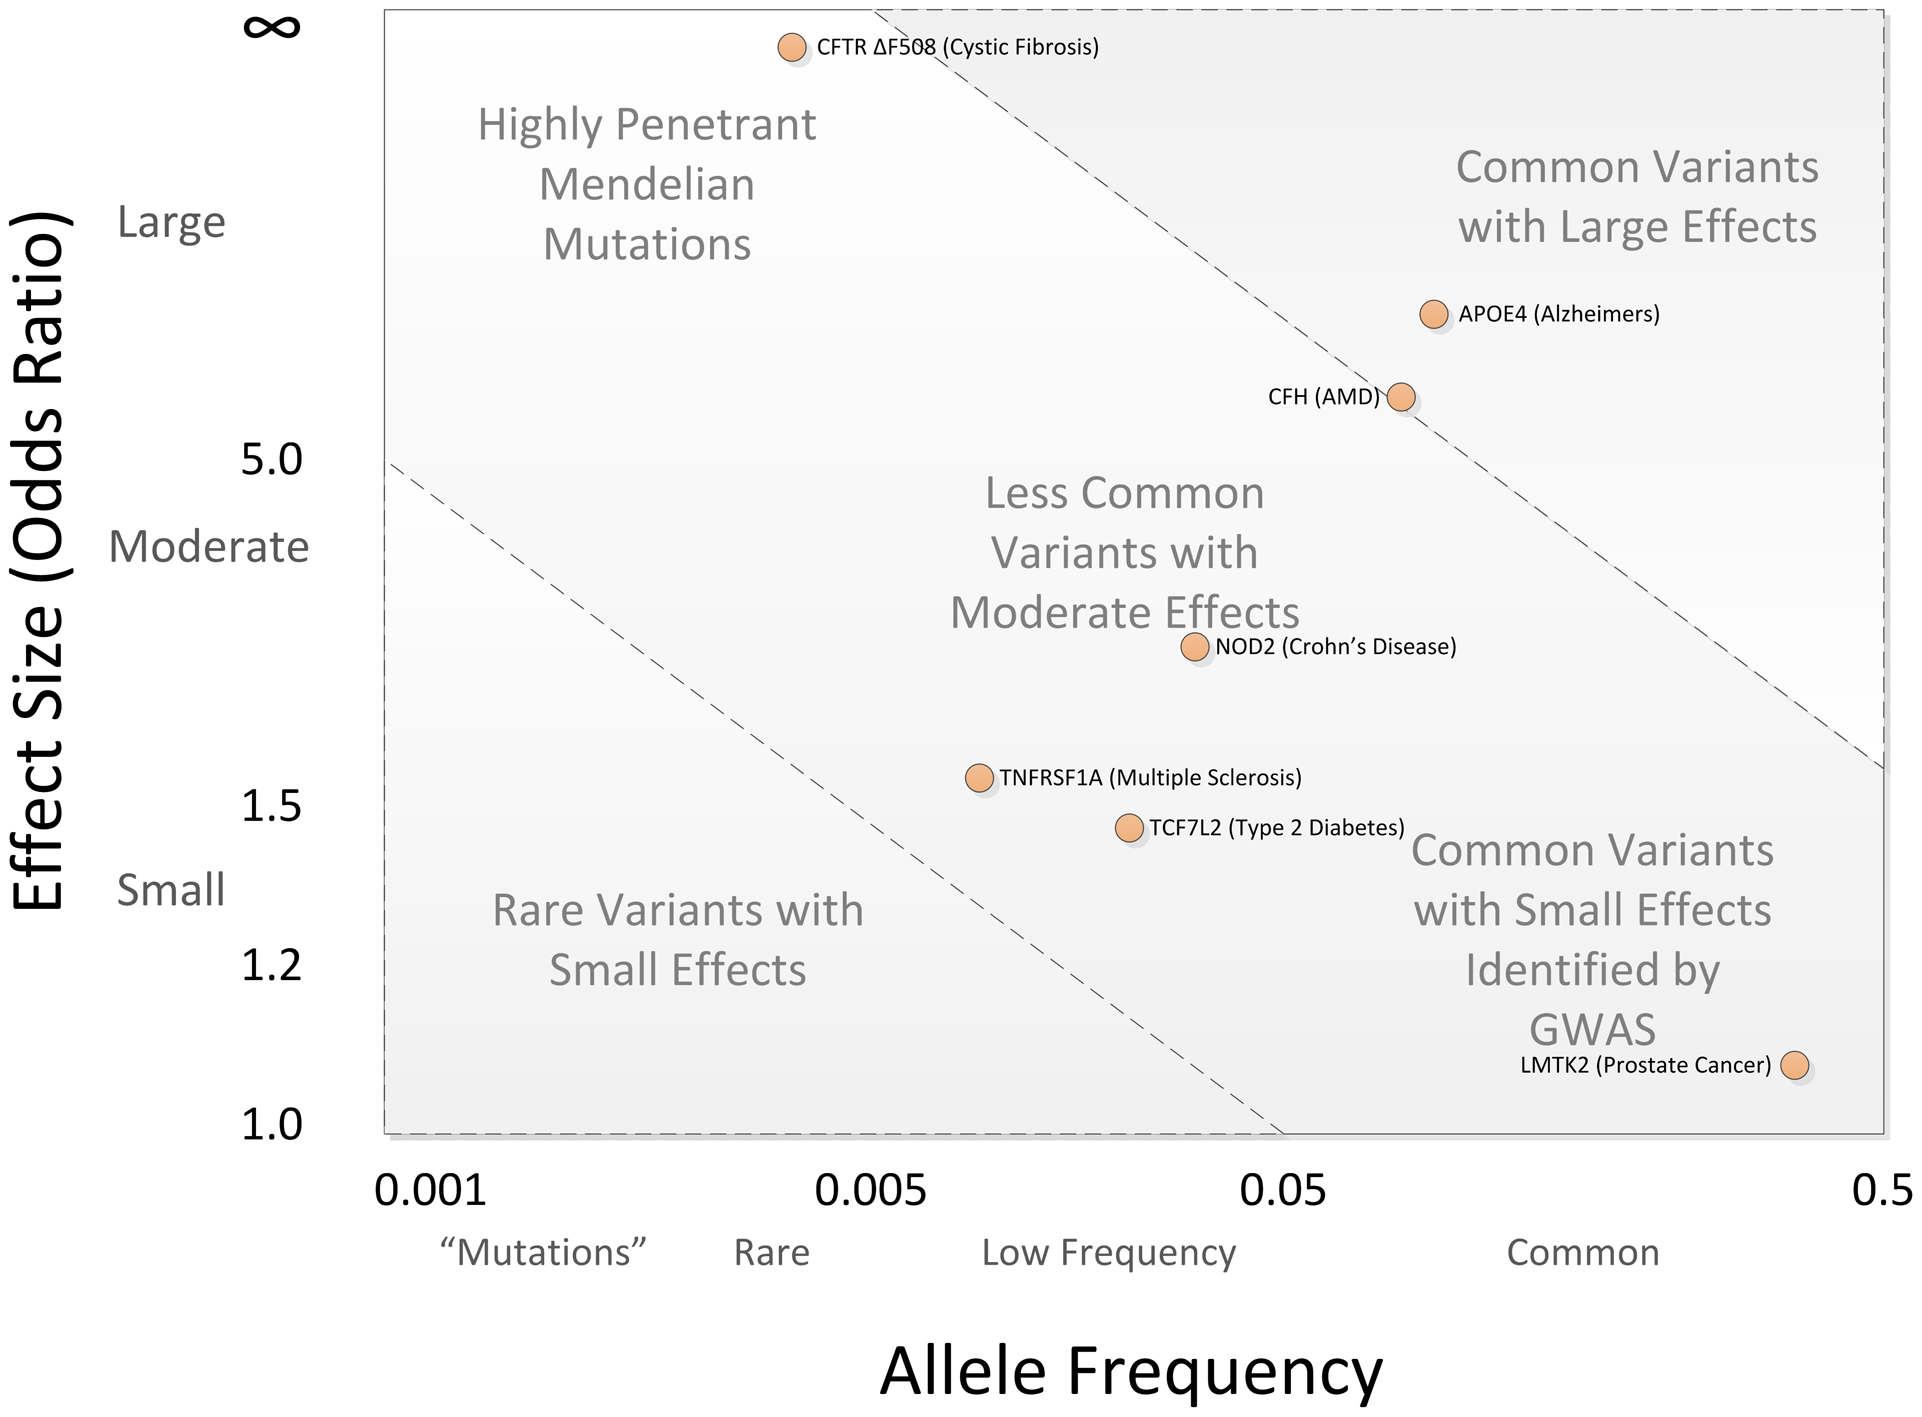
\includegraphics{fig/dl_frequency_vs_effect_size.png}
\caption{\label{fig:size-freq}Relationship between the minor allele frequency of an allele, and its effect size. As a consequence of evolutionary forces, highly deleterious alleles which cause Mendelian diseases are infrequent, while alleles with small effects that increase slightly the susceptibility to a complex disease are more widespread. Figure adapted from Bush and Moore (\protect\hyperlink{ref-bush_chapter_2012}{2012}), licensed under CC BY.}
\end{figure}

Because the risk alleles have such small effect sizes, they are not under strong purifying selection (Figure \ref{fig:size-freq}). This allows them to be common (\textgreater1-5\% of the population), unlike the mutations causing Mendelian diseases, which are rare, as they strongly decrease the fitness of the individual (Manolio et al. \protect\hyperlink{ref-manolio_finding_2009}{2009}). In consequence, the study of the genetics of complex diseases relies on the \emph{common disease, common variant} hypothesis: common diseases are partly attributable to allelic variants present in more than 1-5\% of the population, which cause, by themselves or in combinations, small increments in risk (1.1 - 1.5-fold). However, another consequence of this limited effect size is that only weak associations between causal variants and phenotypes can be expected. Again, this notion is radically different from Mendelian diseases, where every carrier of the risk allele develops the disease under complete penetrance. Therefore, the study of the genetics of complex diseases requires the identification of many risk variants among the 88 millions known ones (The 1000 Genomes Project Consortium et al. \protect\hyperlink{ref-the_1000_genomes_project_consortium_global_2015}{2015}).

The most common source of genetic variation in humans are single base-pair changes in the DNA sequence, called single-nucleotide polymorphisms or SNPs (The 1000 Genomes Project Consortium et al. \protect\hyperlink{ref-the_1000_genomes_project_consortium_global_2015}{2015}). They usually involve two alleles, meaning that in a population there are two possible base-pairs for a genetic position. SNPs are characterized by their minor-allele frequency, that is, the frequency of the least common allele in the population. Although in this thesis I focused my work on SNPs, other forms of genetic variation exist. These are the structural variants, which involve variation in the structure and the quantitative arrangement of the chromosomes (Spielmann, Lupiáñez, and Mundlos \protect\hyperlink{ref-spielmann_structural_2018}{2018}). Copy number variants (CNVs), a type of structural variants, consist on a repeated segment of the genome, where the specific number of repeats changes from person to person. CNVs are relevant for human health. For instance a neurological disorder known as Huntington's disease ensues when a specific tri-nucleotide in the huntingtin gene is repeated more than 36 times (Macdonald \protect\hyperlink{ref-macdonald_novel_1993}{1993}).

\hypertarget{intro-gwas}{%
\section{Genome-wide association studies}\label{intro-gwas}}

Genome-wide association studies (GWAS) are experiments that explore large cohorts, systematically surveying both a high number of genetic variants and the individuals' phenotype(s) (Bush and Moore \protect\hyperlink{ref-bush_chapter_2012}{2012}). Their goal is to find associations between genotypes and the studied phenotype. These associations might lead to earlier diagnoses, choices of treatment appropriate for a patient's genetic background, and better understanding of the etiology of the disease. For that purpose, a classical GWAS involves a statistical test of association between each variant and the phenotype. Often that statistical test is a logistic regression, which allows using additional variables that might act as confounders. For instance, for a SNP \(i\):

\begin{equation}
logit \left(p_i\right) = \alpha + \beta_i g_i + \gamma X
\label{eq:gwas-logreg}
\end{equation}

where \(g_i\) is the vector of genotypes at SNP \(i\), \(\beta_i\) is the coefficient, and \(X\) and \(\gamma\) are respectively the matrix of covariates and the vector with the covariates' coefficients. A statistical test can be conducted on the value of \(\beta\) by transforming it into a Z-score. In order to evaluate the significance of the associated P-value, an appropriate threshold which accounts for multiple testing is needed. Often, that P-value is chosen by setting the family-wise error rate to 0.05 i.e.~\(0.05/\text{\# SNPs}\) (e.g.~10\textsuperscript{-7} if 500,000 SNPs are tested). Then, genome-wide significant SNPs undergo a follow-up study on an independent cohort.

The 1000 Genome Projects catalogued 84.7 million SNPs across multiple human populations (The 1000 Genomes Project Consortium et al. \protect\hyperlink{ref-the_1000_genomes_project_consortium_global_2015}{2015}). However GWAS do not need to survey all of them to obtain a representative view of the genome. Instead, they exploit the correlations between the variants consequence of the genetic history, a phenomenon known as linkage disequilibrium (LD). Thanks to LD, GWAS survey the whole genome in an inexpensive fashion using SNP arrays that contain only a small fraction of the known variants (Visscher et al. \protect\hyperlink{ref-visscher_10_2017}{2017}). In consequence, the SNPs associated with a disease are likely not the causal ones, but SNPs close to the causal variants, and hence in LD with them.

Since the first GWAS in the late 2000s, more than 5,600 studies have shed light into the genetics of complex traits, identifying more than 70,000 variant-trait associations (Buniello et al. \protect\hyperlink{ref-buniello_nhgri-ebi_2019}{2019}). From this community effort we took a few lessons about the architecture of complex traits. First, GWAS confirmed the infinitesimal model in all studied complex traits, whose variance can only be explained but by many loci with small effect sizes (Visscher et al. \protect\hyperlink{ref-visscher_10_2017}{2017}). Such explanatory variants tend to be located in chromatin that is open and expressed in the tissues relevant for the disease (Boyle, Li, and Pritchard \protect\hyperlink{ref-boyle_expanded_2017}{2017}). Also, even genes functionally implicated in the disease explain a small fraction of the trait variance (Boyle, Li, and Pritchard \protect\hyperlink{ref-boyle_expanded_2017}{2017}). In fact GWAS has revealed widespread pleiotropy, as the same genomic regions are often found in association to multiple traits (Visscher et al. \protect\hyperlink{ref-visscher_10_2017}{2017}). This has profound implications, showing how interrelated different biomolecules are. In fact, holistic models that add nuances to the infinitesimal model have been suggested, like the \emph{omnigenic model} (Boyle, Li, and Pritchard \protect\hyperlink{ref-boyle_expanded_2017}{2017}). This model postulates that only a few core genes are directly implicated in the disease, and alterations on them have a strong effect. But alterations in many other, unrelated, genes can also lead to disease as they propagate through biological networks to affect the functionality of those core genes. A more complete view of biological networks and disease is available in Chapter \ref{genesis}.

\hypertarget{intro-gwas-challenges}{%
\subsection{Challenges}\label{intro-gwas-challenges}}

The discovery of the genetic basis of complex diseases is hindered by several intrincacies in both the GWAS setting and the underlying biology. That is why, despite its success in identifying associated variants, all of them together do not explain the whole genetic variance of the disease. Possible explanations include the involvement of a large number of common variants with small effects; of rare variants with large effects not covered in GWAS; of epistasis; and of unaccounted gene-environment interactions (Manolio et al. \protect\hyperlink{ref-manolio_finding_2009}{2009}). My thesis involved developing methodologies that tackle these challenges, which I present below.

\hypertarget{low-statistical-power}{%
\subsubsection{Low statistical power}\label{low-statistical-power}}

Due to the low effects sizes implied by the common disease / common variant hypothesis, GWAS would require very large sample sizes. Yet, for practical limitations, they have traditionally remained in the thousands, with the latest studies raising them up to hundreds of thousands (Sudlow et al. \protect\hyperlink{ref-sudlow_uk_2015}{2015}). However, the number of biomarkers required to scan the whole genome is even larger, from hundreds of thousands to millions. In consequence, GWAS is conducted in an ultradimensional setting which, jointly with the small effect sizes, leads to low statistical power (Wray et al. \protect\hyperlink{ref-wray_pitfalls_2013}{2013}; Visscher, Hill, and Wray \protect\hyperlink{ref-visscher_heritability_2008}{2008}; Button et al. \protect\hyperlink{ref-button_power_2013}{2013}). Statistical power also takes a hit due to the partial correlations between the tests, as multiple test correction procedures like Bonferroni consider the statistical tests independent, and hence overcorrect (Wang, Cordell, and Van Steen \protect\hyperlink{ref-wang_statistical_2018}{2018}). Statistical power can be further reduced when the causal SNPs are in weak LD with the closest genotyped variants, for instance if they are rare, and when the phenotype is heterogeneous (Visscher et al. \protect\hyperlink{ref-visscher_10_2017}{2017}), as is common in complex diseases. This has several implications. First, that by definition we have a small chance of discovering effects that are true. Second, it raises the probability of a discovery to be a false positive. Third, when an underpowered study discovers a true effect it is more likely to overestimate its effect size. One practical consequence of this low power in GWAS is the difficulty to reproduce results (Visscher, Hill, and Wray \protect\hyperlink{ref-visscher_heritability_2008}{2008}).

\hypertarget{encoding}{%
\subsubsection{Choice of encoding}\label{encoding}}

The most commonly used association tests in GWAS require making assumptions on the mode of action of the SNPs (dominance, codominance, etc.). For instance, the logistic regression presented in Equation \eqref{eq:gwas-logreg} needs a single number that represents the two alleles of each individual. Converting the genotype into such a number is known as \emph{encoding a genotype}. There are several such encodings, and its choice have implications on the study: choosing an encoding which diverges from how the SNP truly acts will reduce the statistical power (Romagnoni et al. \protect\hyperlink{ref-romagnoni_comparative_2019}{2019}). A common one is the additive encoding, which assumes that the minor allele is responsible for the phenotype, proportionally to the number of copies; hence, the major allele in homozygosis is represented by a 0, the heterozygous genotype by a 1, and the minor allele in homozygosis by a 2. In Appendix \ref{block-hsic-lasso} we explore a feature selection algorithm which, when applied to GWAS, makes no assumptions on the mode of action of the SNP.

\hypertarget{estimating-individual-risk}{%
\subsubsection{Estimating individual risk}\label{estimating-individual-risk}}

Once the genetic architecture is fully understood, it will be possible to estimate the full genetic component of a patient. This involves moving moving from population-level associations, to an individual assessment (Wray et al. \protect\hyperlink{ref-wray_pitfalls_2013}{2013}). Conventionally these are done through polygenic risk scores, which consist on a linear combination of genotypes from the associated loci in a patient, weighted by their effect sizes. However, their utility is far from clinical applications (Visscher et al. \protect\hyperlink{ref-visscher_10_2017}{2017}). In this thesis, I apply machine learning algorithms for sample classification in Chapter \ref{genesis} (Section \ref{results-benchmark}) and in Appendix \ref{block-hsic-lasso}. Also, it is worth stressing that even when the whole genetic architecture of a disease is uncovered, the \(R^2\) of a linear predictor would be upper bounded by the heritability (\(h^2\)). A complete prediction will require, in addition, fully understanding epistasis (Section \ref{gwais}), environmental effects, and the interactions between environment and genetics.

\hypertarget{pop-structure}{%
\subsubsection{Population structure}\label{pop-structure}}

As explained before, the GWAS exploits LD to avoid genotyping all known variants. However, these correlations between SNPs depend on the evolutionary history of each sample, and hence are population specific. Therefore, GWAS designs must account for samples with different ancestries or, in other words, capture the population structure in the data. Failure to do so might lead to overestimating allelic and genotypic frequencies, reducing statistical power and producing spurious associations (Wang, Cordell, and Van Steen \protect\hyperlink{ref-wang_statistical_2018}{2018}). Population structure can be captured by the principal components of the genotype matrix, and hence they are often used to account for it (Price et al. \protect\hyperlink{ref-price_principal_2006}{2006}). For instance, a logistic regression using the main principal components as covariates is often used to obtain measures of association at the SNP level correcting by potentially confounding population structure (Michailidou et al. \protect\hyperlink{ref-michailidou_genome-wide_2015}{2015}, \protect\hyperlink{ref-michailidou_association_2017}{2017}; Ellinghaus et al. \protect\hyperlink{ref-ellinghaus_analysis_2016}{2016}).

Another consideration is that most GWAS have been carried out on populations of European ancestry, which have a reduced variability in comparison to other human populations (Visscher, Hill, and Wray \protect\hyperlink{ref-visscher_heritability_2008}{2008}). In fact, studies on non-European populations have yielded a big number of new, intriguing variants.

\hypertarget{intro-interpretability}{%
\subsubsection{Interpretability}\label{intro-interpretability}}

By design, a genotyped SNP acts as a tag for the region in the genome in LD with it. Hence, even if that ``tag SNP'' shows statistical association with a disease, fine-mapping studies are needed to pinpoint the specific SNP that gives the susceptibility to it. From a computational perspective, a frequent strategy to link tag SNPs to a function is identifying the genes under the influence of their genomic region (Lehne, Lewis, and Schlitt \protect\hyperlink{ref-lehne2011snps}{2011}; Jorgenson and S Witte \protect\hyperlink{ref-Jorgenson}{2006}), as those are considered the functional unit of inheritance. For instance, a SNP might affect a gene by provoking an amino acid change in the protein product, or altering its gene expression or its splicing. Yet, mapping genomic regions to the genes they might influence is not trivial. In the literature, we find three ways of of doing so. The first one is the physical mapping, which maps that region to the genes whose genomic coordinates overlap with it. Often the gene boundaries are expanded by a fixed number of kilobases, as SNPs in promoters or nearby enhancers can affect gene expression (Segrè et al. \protect\hyperlink{ref-segre_common_2010}{2010}). Nonetheless, physical mapping can be ambiguous due to the overlap between genes (as I illustrate in Section \ref{results:consensus}). The second SNP-gene mapping is through gene expression regulation, when SNPs in the associated genomic region are significantly associated to the expression of a gene. Such loci are known as eQTL. In this regard, the GTEx project (GTEx Consortium \protect\hyperlink{ref-gtex_consortium_genetic_2017}{2017}), a project that genotypes multiple human subjects and extracts expression information from their different tissues, is a useful source of tissue-specific eQTL. Gene expression mapping is not exempt of the overlap problem that occurs in the physical mapping. Solutions which consider LD patterns and the association across the whole genomic region have been proposed (Liu et al. \protect\hyperlink{ref-liu_abundant_2019}{2019}). The third SNP-gene mapping is based on the 3D structure of the genome, which causes distant genomic regions to be close in space (Spielmann, Lupiáñez, and Mundlos \protect\hyperlink{ref-spielmann_structural_2018}{2018}). In this situation, SNPs in a genomic region are associated to neighboring genes in the tridimensional space.

Once a set of SNPs is reliably mapped to a gene, multiple tests extist to aggregate their results into a gene statistic and measure the association of the gene as a whole with the disease. Aggregation of such SNP statistics into gene statistics is likely to increase the statistical power when dealing with complex diseases (Wu et al. \protect\hyperlink{ref-wu2010novel}{2010}). Multiple approaches exist, like SKAT (Wu et al. \protect\hyperlink{ref-wu_rare-variant_2011}{2011}), VEGAS2 (Mishra and Macgregor \protect\hyperlink{ref-mishra_vegas2:_2015}{2015}), or COMBAT (Wang et al. \protect\hyperlink{ref-wang_combat:_2017}{2017}).

\hypertarget{intro-epistasis}{%
\section{Epistasis}\label{intro-epistasis}}

Epistasis is the phenomenon where the effect of one locus on the phenotype depends on the state of one or more additional loci. It has two variants: biological and statistical (Moore and Williams \protect\hyperlink{ref-moore_traversing_2005}{2005}). Biological epistasis refers to the physical interaction occurring between the loci, for instance via their protein products. It is partly a consequence of the redundancy of biological mechanisms, which requires alterating multiple sites in order to alter their broader biological function (Niel et al. \protect\hyperlink{ref-niel_survey_2015}{2015}). Multiple cases of biological epistasis contributing to phenotypes in model organisms have been reported in the literature (Mackay \protect\hyperlink{ref-mackay_epistasis_2014}{2014}). Statistical epistasis, by contrast, is the observation that the association between one locus and the phenotype changes across the level of the other locus. In essence, statistical epistasis refers to the biological epistasis detectable at the population level. In this regard, links between epistasis and complex diseases like Alzheimer's disease (Combarros et al. \protect\hyperlink{ref-combarros_epistasis_2009}{2009}), inflammatory bowel disease (Cho et al. \protect\hyperlink{ref-cho_identification_1998}{1998}) and hypertension (Kimura et al. \protect\hyperlink{ref-kimura_multilocus_2012}{2012}) have been found. As in this thesis I worked exclusively in the detection of the latter kind, for brevity's sake I will refer to it simply as \emph{epistasis}.

Despite the links between epistasis and complex disease mentioned above, estimating the magnitude of its contribution to complex diseases in humans is hard (Gusareva and Van Steen \protect\hyperlink{ref-gusareva_practical_2014}{2014}). Nonetheless, Zuk et al. (\protect\hyperlink{ref-zuk_mystery_2012}{2012}) proposed that incorrectly accounting for epistasis might be behind the so-called \emph{missing heritability} of complex traits. Additionally, studies of traits in model organisms suggest that epistasis plays a key role of their genetic architecture (Mackay \protect\hyperlink{ref-mackay_epistasis_2014}{2014}). This motivates further studying the involvement of epistasis in complex diseases.

\hypertarget{gwais}{%
\section{Genome-wide association interaction studies}\label{gwais}}

Genome-wide association interaction studies (GWAIS) share the experimental design with GWAS, but focus on the detection of epistasic associations. The identification of gene-gene interactions is crucial to understand the functional basis of the association: if two interacting SNPs alter the same gene, and both alterations are required to modify its function, if they affect different genes from the same pathway, from two different pathways that cross-talk, etc. As opposed to GWAS, no standard GWAIS protocol exists yet, although some general recommendations have been issued (Gusareva and Van Steen \protect\hyperlink{ref-gusareva_practical_2014}{2014}; Ritchie and Van Steen \protect\hyperlink{ref-ritchie_search_2018}{2018}).

Due to their similar experimental design, GWAIS and GWAS share the challenges outlined in Chapter \ref{intro-gwas-challenges}. Nonetheless, such problems are often aggravated in GWAIS. For instance, a larger number of tests implies a further reduction of the statistical power. Interpretation is also more complicated, as two or more SNPs need to be mapped to their respective genes (Gusareva and Van Steen \protect\hyperlink{ref-gusareva_practical_2014}{2014}). However it requires two additional considerations, related to the multiple genetic scenarios in which epistasis can occur. As illustration, Li and Reich (\protect\hyperlink{ref-li_complete_2000}{2000}) estimated that there are 50 different fully penetrant disease models involving two loci in epistasis. The first consideration is that a number of arbitrary choices must be made, like the order of the explored interactions, whether to pre-filter the data according to function or detectable main effects, or the genetic encoding (see Section \ref{encoding}) (Romagnoni et al. \protect\hyperlink{ref-romagnoni_comparative_2019}{2019}). For instance, fourth order epistasis involves four different loci jointly contributing to a phenotype. Nonetheless, as the number of interactions grows exponentially with the epistasis order, most methods and studies focus on second order epistasis. The second consideration is that epistasis introduces the challenge of quantifying and assessing the significance of an statistical interaction. Multiple strategies to detect epistasis have been proposed, from logistic regression with an interaction term to deep learning. (Niel et al. (\protect\hyperlink{ref-niel_survey_2015}{2015}) is a comprehensive review of the main epistasis detection strategies.) In general, this diversity comes from tackling different aspects of the computational and statistical issues that arise from the large number of potential interactions. For instance, logistic regression with an interaction term is an exhaustive method with a parallelized implementation (Chang et al. \protect\hyperlink{ref-chang_second-generation_2015}{2015}), but makes strong assumptions on the underlying relationship between the genotype and the phenotype. Hence, statistical power is compromised when that model is inaccurate. On the other hand, MDR (Moore et al. \protect\hyperlink{ref-moore_flexible_2006}{2006}) is model-free and exhaustive, but is limited to case-control phenotypes and its inability to compute P-values analytically makes it slower. In Chapter \ref{epi-network} we examine different epistasis detection methods.

\hypertarget{diseases-studied-in-this-thesis}{%
\section{Diseases studied in this thesis}\label{diseases-studied-in-this-thesis}}

The bulk of my work in this thesis revolved around two complex diseases: familial breast cancer and inflammatory bowel disease.

\hypertarget{breast-cancer}{%
\subsection{Breast cancer}\label{breast-cancer}}

Cancer is the name of a collection of related diseases. Specifically, all cancers undergo an uncontrolled proliferation of the patient cells, which spread into surrounding tissues. In a normal organism, cells grow and divide to maintain the tissue. As cells grow old, or accumulate too much damage, they undergo cell death and new cells will take their place. However, in cancer, this orderly process breaks down. Cells refuse to die when they get old, or accumulate damage. New cells are formed even if they are not needed. In consequence they form purpose-less growths called tumors.

This abnormal behavior occurs as consequence of the alteration of crucial genes. These alterations can be inherited from our parents, or acquired during our lifetime, due to replication errors or exposure to DNA-damaging substances. As with any other phenotypic trait, the likelihood of developing cancer is determined by the interplay between the genetic background and the environment: genetic backgrounds may favor or hinder the acquisition of mutations, and so do environmental factors.

Breast cancer occurs when breast cells undergo this uncontrolled proliferation. In most of the cases they begin in the ducts that carry the milk to the nipple. However the tumor can originate in other tissues, mainly the milk-producing gland.

Breast cancer is the second most commonly diagnosed cancer among women, after non-melanoma skin cancer. It is also the second leading cause of cancer deaths after lung cancer. It is mostly a women's disease: only about 1\% of the diagnosed cases are in men. Among the most important risk factors for breast cancer we can highlight age, family history, reproductive history, usage of oral contraceptives and exposure to radiation. Most breast cancers occur after age 50.

Breast cancer is a very heterogeneous disease: while all the tumors appear in the same organ, the tissue where they originate, the molecular mechanism involved, the response to therapy, etc. vastly differ. In general, clinical decisions are based on the expression of 3 molecular markers: the expression of the endocrine receptors for estrogen and progesterone (ER and PgR, respectively) and the expression of the HER2 gene. The proteins these three genes code for are targets for chemotherapy. Based on the results, we distinguish three main breast cancer subtypes: hormone receptor positive, HER2 positive and triple negative.

\begin{itemize}
\tightlist
\item
  Hormone receptor positive (HR+): HR+ tumors include the tumors expressing ER and/or PR, which respectively depend on estrogen and/or progesterone to grow. They happen mostly in postmenopausal women. HR+/HER2- also known as LuminalA are the majority of breast cancers (60-75\%) and they present the best prognosis.
\item
  HER2 positive (HER2+): HER2+ tumors depend on the protein HER2/neu (human epidermal growth factor receptor 2) to proliferate, which they over-express. HR+/HER2+ (also known as LuminalB) constitute 10\% of the cases, while HR-/HER2 (also known as HER2-enriched) involves 5\% of them. There are a couple of very effective drugs against it.
\item
  Triple-negative: Triple-negative tumors lack the expression of all three of ER, PgR and HER2. These patients present a worse prognosis than the rest, due to the aggressiveness of the tumor and the lack of a clear molecular target. Still, the main treatment is chemotherapy.
\end{itemize}

In the mid-19th century a French medical doctor, Pierre Paul Broca, reported for the first time a case of familial breast cancer (Nielsen, Overeem Hansen, and Sørensen \protect\hyperlink{ref-nielsen_hereditary_2016}{2016}). Indeed, his wife acquired breast cancer, as many women in her family had for, at least, 4 generations. Cases of familiar breast cancer usually occur in women younger than 50 years, and bilateral primary breast tumors are frequent. Epidemiological studies later quantified the relative risk conferred by a the presence of multiple breast cancers in the family at 2.7. Moreover, they exhibit a higher likelihood of acquiring triple-negative breast cancer.

It was not until the late 20th century that two genes involved in DNA repair, \emph{BRCA1} and \emph{BRCA2}, were associated with hereditary breast and ovarian cancer (HBOC). Some mutations in these genes increase the risk of developing breast cancer, giving respectively a 57--65\% or 45--55\% risk of developing breast cancer by age 70 among women. For that reason, \emph{BRCA1} and \emph{BRCA2} mutations are rare in most populations (1 of 400).

HBOC follows an autosomal dominant inheritance pattern. While approximately 5--10\% of all patients with breast cancer exhibit a monogenic predisposition to breast and ovarian cancer, only about 25\% of them harbor \emph{BRCA1/2} mutations. An additional 23 genes have been associated with familial breast and/or ovarian cancer (Table \ref{tab:hboc-genes}).

Nearly all known HBOC susceptibility genes encode tumor suppressors that participate in genome stability pathways (homologous recombination repair, replication fork stability, transcription--replication collisions, mismatch repair, and DNA damage signaling, checkpoints and cell death; see Appendix \ref{hboc-genes} for more information).

\hypertarget{genesis-dataset}{%
\subsubsection{The GENESIS dataset}\label{genesis-dataset}}

In Chapter \ref{genesis}, I search for risk factors for familial breast cancer
in the French population on the he GENE Sisters (GENESIS) study
(Sinilnikova et al. \protect\hyperlink{ref-sinilnikova_genesis:_2016}{2016}). Index cases are patients with infiltrating
mammary or ductal adenocarcinoma, who had a sister with breast cancer,
and who have been tested negative for \emph{BRCA1} and \emph{BRCA2} pathogenic
variants. Controls are unaffected colleagues and/or friends of the
cases, born around the year of birth of the corresponding case (\(\pm 3\)
years). We focused on the 2,577 samples of European ancestry, of which
1,279 are controls and 1,298 are cases. The genotyping was performed
using the iCOGS array, a custom Illumina array designed to study genetic
susceptibility of hormone-related cancers (Sakoda, Jorgenson, and Witte \protect\hyperlink{ref-sakoda_turning_2013}{2013}). It
contains 211,155 SNPs, including SNPs putatively associated with breast,
ovarian, and prostate cancers, SNPs associated with survival after
diagnosis, and SNPs associated to other cancer-related traits, as well
as functional candidate variants in selected genes and pathways.

\hypertarget{inflammatory-bowel-disease}{%
\subsection{Inflammatory bowel disease}\label{inflammatory-bowel-disease}}

Inflammatory bowel disease (IBD) is a group of complex diseases that, as the name indicates, share a common theme of inflammation of the intestines. The two main subtypes are ulcerative colitis and Chron's disease. Clinically, these two share a lot of the symptoms, mainly intermittent abdominal pain and diarrhea (Liu and Stappenbeck \protect\hyperlink{ref-liu_genetics_2016}{2016}). However, they differ in the specific regions of the digestive tract that get affected, as well as the specific lesions. IBD's incidence worldwide has been continually growing, specially in newly industrialized countries, and after decades of growth it has stabilized in North America, Oceania and Europe (Ng et al. \protect\hyperlink{ref-ng_worldwide_2017}{2017}). In these latter countries the prevalence is slightly above 0.3\%.

The genetic component of IBD was recognized more than a century ago (Ek, D'Amato, and Halfvarson \protect\hyperlink{ref-ek_history_2014}{2014}). However, it was not until 2001 that the first gene, \emph{NOD2}, was linked to IBD susceptibility. Ever since, hundreds of loci have been associated to IBD as well, in positions related to immune system genes, both innate and adaptive (Loddo and Romano \protect\hyperlink{ref-loddo_inflammatory_2015}{2015}; Ellinghaus et al. \protect\hyperlink{ref-ellinghaus_analysis_2016}{2016}; Liu and Stappenbeck \protect\hyperlink{ref-liu_genetics_2016}{2016}). For instance \emph{NOD2}, and other susceptibility genes like \emph{IL23R}, and \emph{PTPN2}, are related to cell signalling in immune cells. However, most of the loci associated to genes are rare variants (\textless{} 0.5\%) with large effect sizes. By contrast, several GWAS have identified very common SNPs (20-50\%) with small effect sizes (odds ratio \textless{} 1.1) (Liu and Stappenbeck \protect\hyperlink{ref-liu_genetics_2016}{2016}), but which do not encode any coding change (Jostins et al. \protect\hyperlink{ref-jostins_hostmicrobe_2012}{2012}). This raises questions about the underlying biology (see Section \ref{intro-interpretability}). For a comprehensive view of the genetics of IBD, interested readers can read Liu and Stappenbeck (\protect\hyperlink{ref-liu_genetics_2016}{2016}) and Loddo and Romano (\protect\hyperlink{ref-loddo_inflammatory_2015}{2015}).

\hypertarget{iibdgc-dataset}{%
\subsubsection{The IIBDGC dataset}\label{iibdgc-dataset}}

In Chapters \ref{epi-snp2gene} and \ref{epi-network}, I search for epistatic interactions giving susceptibility to IBD. Specifically, I examine the largest case-control GWAS on ulcerative colitis and Chron's disease to date (Jostins et al. \protect\hyperlink{ref-jostins_hostmicrobe_2012}{2012}), produced by the International Inflammatory Bowel Disease Genetics Consortium (IIBDGC). The dataset contain 66,280 samples, out of which 32,622 are cases and 33,658 are controls. The Immunochip SNP array was used for the genotyping (Cortes and Brown \protect\hyperlink{ref-cortes_promise_2010}{2010}), which contains 196,524 polymorphisms, with a special focus on immunogenetics.

\hypertarget{network-view-of-complex-diseases}{%
\section{Network view of complex diseases}\label{network-view-of-complex-diseases}}

Human biology is notoriously complicated, as sheer numbers demonstrate: to form a 70 kg man, 3.0 \texttimes 10\textsuperscript{13} cells (Sender, Fuchs, and Milo \protect\hyperlink{ref-sender_revised_2016}{2016}) assemble and interact to produce and maintain 79 organs. To achieve that level of complexity, human cells depend on their genetic material, carefully tuned by epigenetics and enabled by a favorable environment. In terms of genetics, the object of my work, a human diploid genome is 6.4 billion base pairs long, and harbors 44,393 genes, of which 20,444 encode for a protein and 23,949 are RNA genes. DNA, proteins and RNA are in constant interplay with each other, with the metabolites, and with the environment. Proteins physically interact with each other in highly specific ways (protein-protein interactions or PPIs). If such interactions are stable enough, proteins can assemble into large complexes to carry out particular functions. But proteins also interact with DNA to regulate gene expression (transcription factor - DNA interactions). And so on: enzymes interact with their metabolites, hormones with their receptors, the individual with their environment, etc. At a fundamental level, a person and their traits are just the emerging pattern born from the interaction of all these factors. Hence, biology, from ecosystems to molecular biology, cannot be understood if not as an interplay. Mindful of this, and enabled by the omics technologies of the 21st century, researchers have striven to capture and understand these relationships. The goal of \emph{systems biology} is achieving a global understanding of the complex interplay that drives biology. Among all the possible biological relationships, in this thesis I focus on protein-protein interactions, including protein complexes, as their coverage is larger and their properties better understood. Such interactions are available in databases like HINT (Das and Yu \protect\hyperlink{ref-das_hint_2012}{2012}), The BioGRID (Oughtred et al. \protect\hyperlink{ref-oughtred_biogrid_2019}{2019}) or IntAct (Hermjakob \protect\hyperlink{ref-hermjakob_intact_2004}{2004}).

Relationships between pairs of entities can be mathematically formalized as a network, which makes them analytically approachable. In such networks, often proteins or genes are the nodes, which are connected by edges in a pairwise fashion when they are functionally related. Although the edges might have directionality, often PPIN are undirected, as the direction of the edges is often unknown (transitory interactions), or inexistent (co-complexes) (Barabási, Gulbahce, and Loscalzo \protect\hyperlink{ref-barabasi_network_2011}{2011}). The field of systems biology relies on the assumption that the network accurately captures the context a biomolecule requires to carry out its biological function. We can distinguish three levels of network properties: properties of individual nodes (local), the joint properties of groups of nodes (mesoscale), and the properties over the whole network (global). Indeed, at all three levels biological networks are structured, very differently from random networks (Barabási, Gulbahce, and Loscalzo \protect\hyperlink{ref-barabasi_network_2011}{2011}; Chaiboonchoe et al. \protect\hyperlink{ref-Chaiboonchoe2013}{2013}).

At the global level, for instance, the degree, which represents the number of edges per node, follows a power-law distribution (Barabási, Gulbahce, and Loscalzo \protect\hyperlink{ref-barabasi_network_2011}{2011}). This implies that, at the local level, a few genes participate in the majority of the edges. Such nodes are called \emph{hubs}. Importantly, this node property is informative of the gene function: \emph{in utero} essential genes, like knots preventing the network from falling apart, tend to be hubs. An important consequence of the structured degree distribution at the mesoscale level is the emergence of \emph{modules}, subsets of nodes densely interconnected to each other, and sparsely to the rest. A mesoscale property of biological networks is that they have a modular structure i.e.~a strong division into modules. Such modules often constitute functional units within the network, where the nodes jointly contribute to a specific function (Mitra et al. \protect\hyperlink{ref-mitra_integrative_2013}{2013}).

Another global property of a graph is the distribution of distances between pairs of nodes, that is, how many edges must be passed to travel from one node to another. Such is the notion of \emph{path} between nodes. Often we are interested in the \emph{shortest} path, for they reveal the fastest way information can flow from one node to another. An examination of the distribution of shortest paths in biological networks shows that all nodes are close to each other (shortest paths are, in fact, pretty short on average) (Barabási, Gulbahce, and Loscalzo \protect\hyperlink{ref-barabasi_network_2011}{2011}). Such networks are called \emph{small world networks}. This structure makes the flow of information resilient to the removal of nodes or edges (Chaiboonchoe et al. \protect\hyperlink{ref-Chaiboonchoe2013}{2013}), a cause of biological epistasis (Niel et al. \protect\hyperlink{ref-niel_survey_2015}{2015}).

\hypertarget{networks-in-disease}{%
\subsection{Networks in disease}\label{networks-in-disease}}

Examining how biological networks relate to disease, and the topology around disease genes produces a nuanced approach to disease: cut the knot in the center of the web that keeps it all together, and it all will fall off; cut a bunch of peripheral, less important nodes around it, the outcome might be the same. In other words, there are many ways of producing the same disease (Leiserson et al. \protect\hyperlink{ref-leiserson_network_2013}{2013}).

The properties of biological networks enumerated above lay down the foundations of the use of biological networks to study disease genes. For instance, they justify the \emph{local hypothesis}, which expects genes involved in a disease to interact with each other (Barabási, Gulbahce, and Loscalzo \protect\hyperlink{ref-barabasi_network_2011}{2011}). They also justify the \emph{disease module hypothesis}, which expects genes involved in the same disease to share a module. Experimentally, network propagation highlights the differential topological properties of disease genes and biological networks. \emph{Network propagation} refers to methods that use all the possible paths in the network to re-rank the genes on it (Cowen et al. \protect\hyperlink{ref-cowen_network_2017}{2017}). They include heat diffusion, random walk, graph kernels, and even Google's search algorithm. In essence, for these methods, association of a node with a phenotype can be thought of as a volume of water: the more strongly associated, the more voluminous. Generically, each node starts with that initial volume which, iteratively, gets distributed among its neighbors. Equivalently, every node will receive a share from their neighbors'. The expectation is that truly associated genes will be densely interconnected to each other, forming cycles and modules that will keep the water from diffusing to other, uninvolved genes. After a number of steps the volume of water in each node is re-evaluated, and used to re-prioritize the genes. Using network propagation Huang et al. (\protect\hyperlink{ref-huang_systematic_2018}{2018}) recently showcased the differential topological properties of disease genes. Across different biological networks, they were able to retrieve disease-related genes with varying success using only a subset of them through a random walk with restart procedure.

Indeed, disease genes exhibit different properties than non-disease genes (Piñero et al. \protect\hyperlink{ref-pinero_uncovering_2016}{2016}; Cai, Borenstein, and Petrov \protect\hyperlink{ref-cai_broker_2010}{2010}; Furlong \protect\hyperlink{ref-furlong_human_2013}{2013}; Barabási, Gulbahce, and Loscalzo \protect\hyperlink{ref-barabasi_network_2011}{2011}). For starters, disease genes are not hubs (Cai, Borenstein, and Petrov \protect\hyperlink{ref-cai_broker_2010}{2010}; Das and Yu \protect\hyperlink{ref-das_hint_2012}{2012}), but tend to be non-essential genes located towards the periphery. This is coherent with an evolutionary framework, where mutations in essential genes would be highly deleterious, even resulting in embryonic lethality. However, this enrichment is driven mainly by cancer genes (Piñero et al. \protect\hyperlink{ref-pinero_uncovering_2016}{2016}). Additionally, disease genes tend to be \emph{bottlenecks} i.e.~the sole link between many peripheral genes and the rest of the network (Cai, Borenstein, and Petrov \protect\hyperlink{ref-cai_broker_2010}{2010}), suggesting that disease arises when these vulnerable regions of the network break down.

These properties, however, do not affect equally all types of disease genes. Many of the aforementioned properties do not extend to genes identified through GWAS (Cai, Borenstein, and Petrov \protect\hyperlink{ref-cai_broker_2010}{2010}). Differences arise even when comparing genes involved in complex diseases with those involved in Mendelian ones.

\hypertarget{network-guided-approaches-to-disease-study}{%
\subsection{Network-guided approaches to disease study}\label{network-guided-approaches-to-disease-study}}

As exemplified in the previous section, networks can be leveraged on to gain insight of the biology of the disease. Below I summarize several ways of doing that, on which I have worked on during my PhD.

\hypertarget{intro-hs3}{%
\subsubsection{High-score subnetwork search}\label{intro-hs3}}

One of the focuses of my thesis was the study of networks where the nodes are scored by their association to the disease. The scores might come from omics experiments, or from \emph{a priori} knowledge of disease genes. In essence, such methods look for connected subnetworks made of nodes with high scores. Lacking a term broadly agreed upon in the community, I refer to such algorithms as high-score subnetwork search. Although heterogeneous, to some extent all existing approaches are based on the \emph{guilt-by-association principle} (Figure \ref{fig:network-gwas}): nodes nearby other nodes associated to the disease are suspect of being associated themselves, even if their association is non-significant by conventional standards. However, taking only the genes associated with those associated would be prone to false positives, as often networks include edges that are not relevant for the biological problem at hand. Several high-score subnetwork search methods are available in the literature. Essentially, they differ in the considerations they make on what the solution looks like. In Chapter \ref{genesis} we describe a representative set of these methods, critically discuss their performance at biomarker discovery on the GENESIS dataset, and compare their strengths and weaknesses.



\begin{figure}
\centering
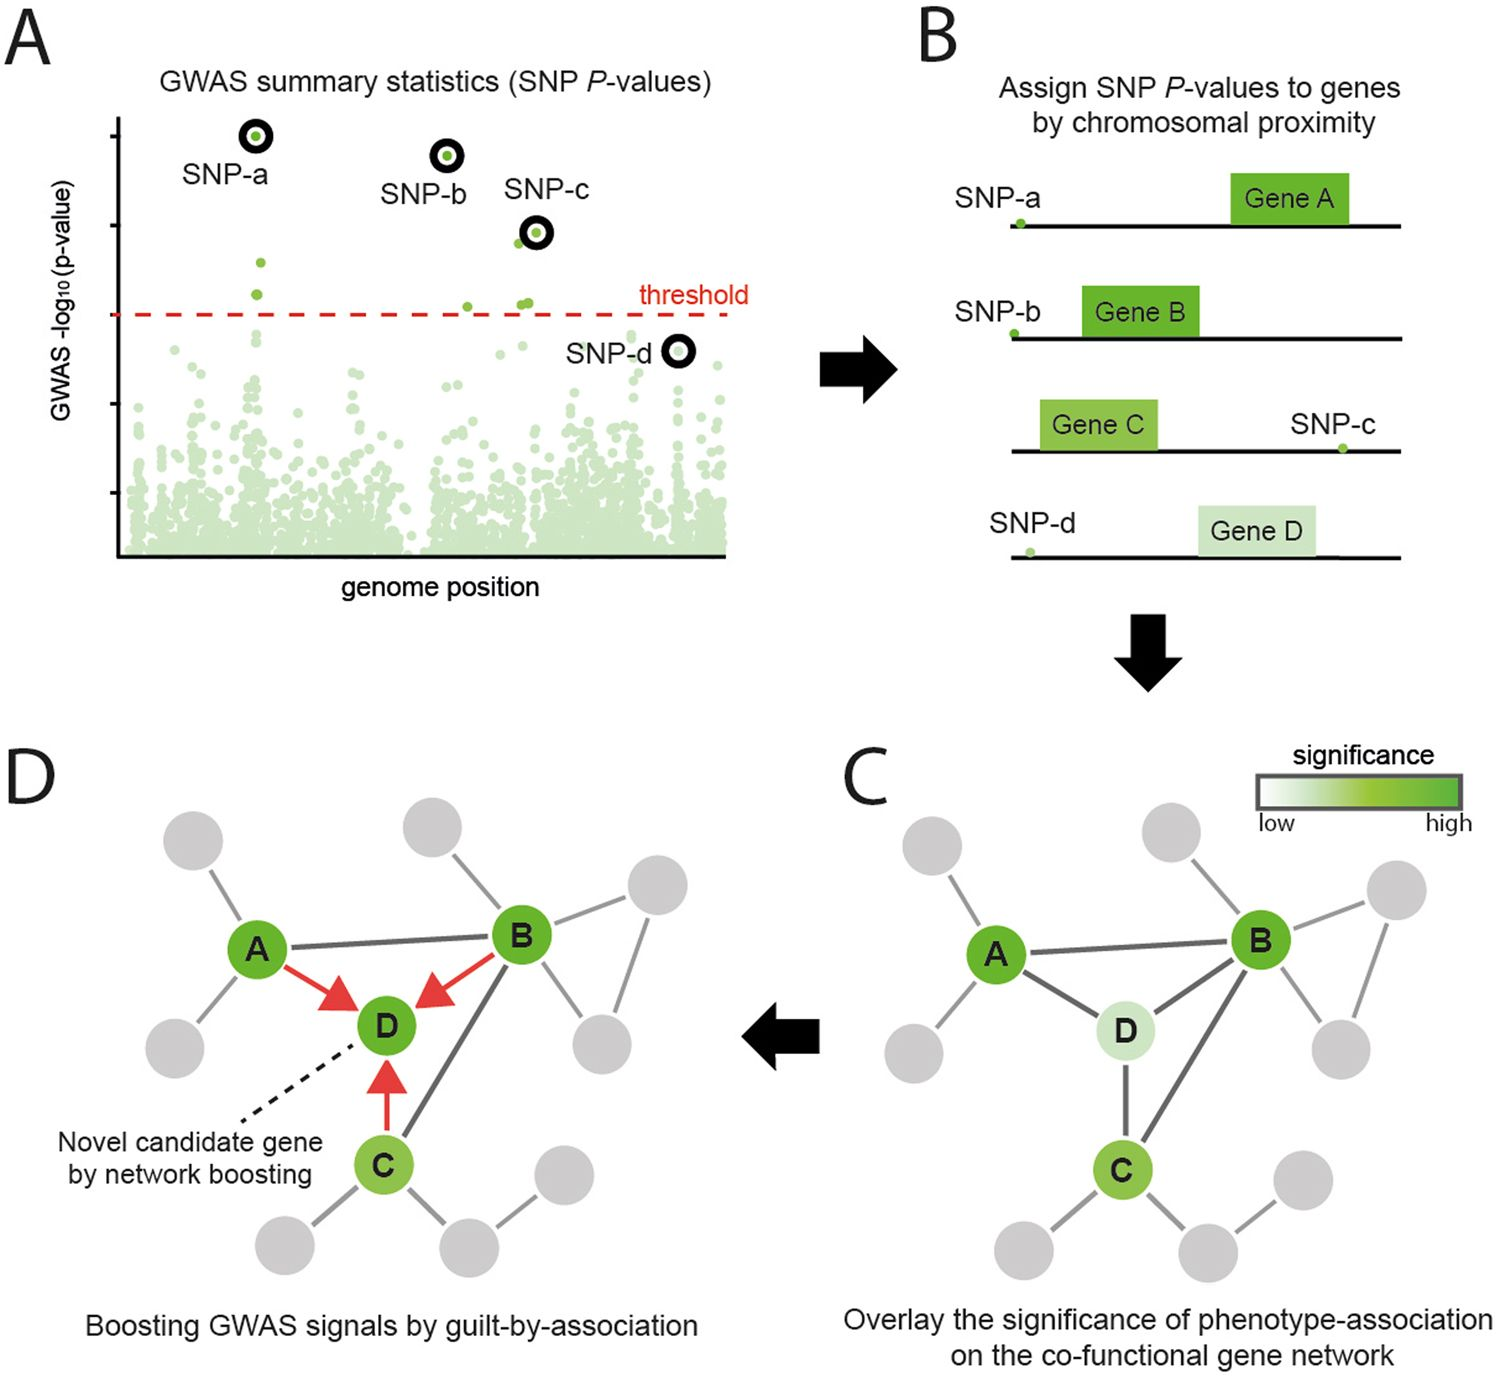
\includegraphics{fig/dl_network_gwas.jpg}
\caption{\label{fig:network-gwas}Overview of the high-score subnetwork search applied to GWAS. \textbf{(A)} From a set of GWAS results, first \textbf{(B)} SNP P-values are assigned to genes (e.g.~by physical mapping). \textbf{(C)} The significance of the phenotype-association for each gene is based on the assigned P-value, which is overlaid on a co-functional network. \textbf{(D)} The significance of each gene is boosted by guilt-by-association, resulting in additional candidate genes (e.g., Gene D) for the phenotype. Figure and caption adapted from Lee and Lee (\protect\hyperlink{ref-lee_aragwab_2018}{2018}), licensed under CC BY 4.0.}
\end{figure}

\hypertarget{module-detection}{%
\subsubsection{Module detection}\label{module-detection}}

In the context of disease, densely interconnected subnetworks (modules) of consistently altered nodes might represent the mechanisms that lead to it. Hence, their identification can provide insights into its etiology. In Appendix \ref{smartas} we apply module detection techniques to a subnetwork of genes with abnormal splicing in cancer.

\hypertarget{aggregation-of-networks}{%
\subsubsection{Aggregation of networks}\label{aggregation-of-networks}}

During my research, often I obtained multiple high-scoring subnetworks using different approaches, which provided complementary perspectives of the same disease. In consequence, I was interested in integrating them into a single subnetwork, which I would analyze. In Chapter \ref{genesis} we discuss a naive way of aggregating subnetworks from different high-score subnetwork search algorithms, were the edges are unweighted. In Chapter \ref{epi-network} we create an epistasis network from interactions from several epistasis detection methods, whose edges are weighed by the confidence they exist.

\hypertarget{contributions}{%
\section{Contributions}\label{contributions}}

The object of my thesis was the methodological study and application of network methods to GWAS data. In essence, networks contain prior information, which can be traded for statistical astringency in our analysis. In other words, if genes strongly associated to a disease, albeit non-significantly so, are interconnected in an underlying biological network, we are more likely to believe they represent a consistently altered biological mechanism.

In collaboration with Nadine Andrieu and Fabienne Lesueur (Institut Curie), and working closely with Christine Lonjou (Institut Curie), I applied six high-score subnetwork search to the GENESIS dataset (Section \ref{genesis-dataset}). Our goal was to find new biomarkers for breast cancer susceptibility. My work on GENESIS is explained in Chapter \ref{genesis}. In summary, I applied six different network-based, biomarker discovery methods to the GENESIS dataset. The methods provide a representative view of the high-score subnetwork search field. We performed a methodological comparison and a benchmark of the methods, highlighting their strengths and weaknesses. Finally, we conclude that combining the methods provide a more complete answer than any of the individual solutions. Our network analysis recovers both genes and genomic regions previously found in association with breast cancer susceptibility, as well as new genes. Importantly, all of those genes are tied in a subnetwork, providing a rationale on how alterations on those genes might lead to disease.

My first approach to the problem involved working on SConES (Azencott et al. \protect\hyperlink{ref-azencott_efficient_2013}{2013}), one of the high-score subnetwork search methods examined in Chapter \ref{genesis}. I give a more detailed explanation of this algorithm, together with my work on it in Chapter \ref{martini}. In summary, I worked on applying SConES to case-control datasets, and strategies to parametrize it. Additionally, in \emph{martini} SConES can take user-provided covariates. Regarding the former, as SConES implemened exclusively the regression version of SKAT (Wu et al. \protect\hyperlink{ref-wu_rare-variant_2011}{2011}; Ionita-Laza et al. \protect\hyperlink{ref-ionita-laza_sequence_2013}{2013}), I implemented two ways of measuring association between a SNP and a binary phenotype. Regarding the latter, SConES has two parameters, \(\eta\) and \(\lambda\), which control the sparsity and the inter-connectedness of the selected SNPs, respectively. Originally the parameters that produced the most stable solution were selected. I explored the impact of penalized-likelihood measures like BIC, AIC, and AICc, which score a set of features based on both their sparsity and the accuracy of a linear classifier built on them. The product of my work is published as \emph{martini} (Climente-González and Azencott \protect\hyperlink{ref-martini}{2019}), an R package published in the peer-reviewed R repository Bioconductor (Huber et al. \protect\hyperlink{ref-bioconductor}{2015}).

In 2019, when I started working on epistasis detection, we established a collaboration with Kristel Van Steen (University of Liège, Belgium). Specifically, I worked closely with Diane Duroux, a PhD student in her research group. Our goal was to build an epistasis gene network of inflammatory bowel disease. I discuss our efforts in this regard in Chapter \ref{epi-network}. For that purpose, we surveyed suitable epistasis detection methods, applied them to the IIBDGC dataset (Section \ref{iibdgc-dataset}), and integrated the solution. However, as a previous step we needed to appropriately map epistatic SNP networks to epistatic gene networks. I describe this work in Chapter \ref{epi-snp2gene}. In summary, we examined and evaluated four different mappings (physical, eQTL, chromatin, and the three together).

In collaboration with Makoto Yamada (RIKEN AIP, Japan) and Samuel Kaski (Aalto University, Finland), I developed block HSIC Lasso, a general-purpose non-linear feature selector. The work involved modifying an existing algorithm, HSIC Lasso, to reduce its memory consumption. On top of that, we worked on both improving its performance and solving numerical issues in edge cases. The algorithm is implemented as the Python package \emph{pyHSICLasso}, available on both PyPI and GitHub. Then, I characterized the algorithm and applied it to several biological datasets. Crucially, three of the datasets were GWAS, which was a milestone in terms of the number of features block HSIC Lasso can handle. Thanks to this work we analyzed the impact of considering non-redundancy and non-linear models when selecting SNPs for patient classification. We describe the algorithm and our conclusions in the article \emph{Block HSIC Lasso: model-free biomarker detection for ultra-high dimensional data} published in the proceedings of the ISMB/ECCB 2019 (Climente-González et al. \protect\hyperlink{ref-climente-gonzalez_block_2019}{2019}). The full manuscript is available in Appendix \ref{block-hsic-lasso}.

Additionally, I worked on the involvement of alternative splicing in cancer with Eduardo Eyras (Australian National University), a continuation of my previous research. During 2016 and early 2017, we prepared the answer to reviewers for the article \emph{The functional impact of alternative splicing in cancer}, which was published in Cell Reports in August 2017 (Climente-González et al. \protect\hyperlink{ref-climente-gonzalez_functional_2017}{2017}). The full manuscript is available in Appendix \ref{smartas}. I also explored evidence of epistasis in cancer, looking for mutual exclusivity between alterations in alternative splicing and somatic mutations. We searched for evidence of mutual exclusivity at both the gene and the pathway level. Among others, we found a compelling pattern in \emph{GATA3}. This finding was published in Cell Reports in March 2018, in the broader article \emph{Systematic analysis of splice-site-creating mutations in cancer} (Jayasinghe et al. \protect\hyperlink{ref-jayasinghe_systematic_2018}{2018}). The full manuscript is available in Appendix \ref{scm}. In addition, I compiled the code required for the analyses in Climente-González et al. (\protect\hyperlink{ref-climente-gonzalez_functional_2017}{2017}), and created a Python package with a clean interface. The package, \emph{spada}, is available in both PyPI and GitHub. This package searches alterations of alternative splicing in a user-provided dataset, and maps them to functional consequences at the protein level. Specifically, such consequences are the removal/addition of functional modules to the protein (e.g.~domains) and the loss or gain of protein-protein interactions. Lastly, I applied \emph{spada} to two leukemia datasets from TARGET, an NIH program that aims to understand the molecular basis of several childhood cancers. This last analysis is still on-going.

Lastly, I carried out my research committed to open, reproducible science. As such, all my projects have an associated, version-controlled, laboratory notebook, which includes as much data as I am allowed to share. All such laboratory notebooks are made out public when the paper is. All the scripts I developed are open source, under permissive MIT license. Specifically, I made an effort to develop project-independent tools, which are useful to anyone which needs similar to the ones I had. These tools are available on GitHub (\url{https://github.com/hclimente/gwas-tools}).

\hypertarget{genesis}{%
\chapter{Combining network-guided GWAS to discover susceptibility mechanisms for breast cancer}\label{genesis}}

The contents of this chapter are based on \emph{Héctor Climente-González, Christine Lonjou, Fabienne Lesueur, GENESIS investigators, Dominique Stoppa-Lyonnet, Nadine Andrieu and Chloé-Agathe Azencott}, Combining network-guided GWAS to discover susceptibility mechanisms for breast cancer (manuscript in preparation). Parts of this work were presented in ASHG 2018 in the poster \emph{Héctor Climente-González, Christine Lonjou, Fabienne Lesueur, GENESIS investigators, Dominique Stoppa-Lyonnet, Nadine Andrieu and Chloé-Agathe Azencott}, Judging genetic loci by the company they keep: comparing network-based methods for biomarker discovery in familial breast cancer.

\begin{chapabstract}{Abstract:}
Systems biology provides a comprehensive approach to biomarker discovery and biological hypothesis building. It does so by jointly considering the statistical association between a gene and a phenotype, and the biological context of each gene, represented as a network. In this chapter we study how six network methods can be used to discover new biomarkers for breast cancer susceptibility by searching subnetworks highly associated to this  phenotype. We interrogate a familial breast cancer genome-wide association study (GWAS) focused on BRCA1/2 negative French women. By trading statistical astringency for biological meaningfulness, most network methods get more compelling results than standard SNP- and gene-level analyses, recovering causal subnetworks tightly related to cancer susceptibility. We perform an in-depth benchmarking of the methods with regards to size of the solution subnetwork, their utility as biomarkers, and the stability and the runtime of the methods. Interestingly, a combination of solution subnetworks provided a concise subnetwork of 93 genes, enriched in known breast cancer susceptibility genes (BABAM1, BLM, CASP8, FGFR2, and TOX3, Fisher's exact test P-value = $7.8 \times 10^{-5}$) and more central than average. Additionally, it includes subnetworks of mechanisms related to cancer, like protein folding (HSPA1A, HSPA1B, and HSPA1L) or mitochondrial ribosomes (MRPS30, MRPS31, MRPS18B). We also observed a general dysregulation in the neighborhood of COPS5, a gene related to multiple hallmarks of cancer.
\end{chapabstract}
\vskip 0.2in
\begin{chapabstract}{Résumé :}
La biologie des syst\`emes permet de d\'evelopper une approche globale de la 
recherche de biomarqueur et de la construction d'hypoth\`eses biologiques. 
Elle rend en effet possible de replacer l'association statistique entre 
un g\`ene et un ph\'enotype dans le contexte biologique de ce g\`ene, gr\^ace \`a 
des r\'eseaux biologiques. Dans ce chapitre, nous \'etudions l'applicabilit\'e 
de six m\'ethodes bas\'ees sur des r\'eseaux pour la d\'ecouverte de nouveaux 
biomarqueurs de susceptibilit\'e dans le cancer du sein, en cherchant des 
sous-r\'eseaux fortement associ\'es \`a un ph\'enotype. Nous \'etudions une GWAS 
sur le cancer du sein familial, concernant des femmes françaises BRCA1/2 
n\'egatives. La plupart de ces m\'ethodes permettent d'obtenir des r\'esultats 
plus convaincants que des analyses standard, et retrouvent des 
sous-r\'eseaux fortement li\'es \`a la susceptibilit\'e dans le cancer. Nous 
proposons une comparaison d\'etaill\'ee des m\'ethodes en terme de taille de 
la solution, de son utilisabilit\'e comme biomarqueur, de stabilit\'e ainsi 
que de temps de calcul. Nous combinons les sous-r\'eseaux retourn\'es par 
ces m\'ethodes en un r\'eseau restreint \`a 93 g\`enes, enrichi en g\`enes de 
susceptibilit\'e au cancer du sein connus, (BABAM1, BLM, CASP8, FGFR2, and 
TOX3, p-valeur du test exact de Fisher = $7.8 \times 10^{-5}$), et plus 
central que la moyenne. De plus, ce r\'eseau contient des sous-r\'eseaux de 
m\'ecanismes li\'es au cancer, tels que le repliement des prot\'eines (HSPA1A, 
HSPA1B, and HSPA1L) ou les ribosomoes mitochondriaux (MRPS30, MRPS31, 
MRPS18B). Nous observons aussi une dysr\'egulation g\'en\'eralis\'ee au 
voisinage de COPS5, un g\`ene li\'e \`a plusieurs caract\'eristiques 
fondamentales du cancer.
\end{chapabstract}

\hypertarget{introduction}{%
\section{Introduction}\label{introduction}}

Network-based biomarker discovery methods provide a comprehensive
statistical framework which includes the structure of biological data
tackle the the challenges in the GWAS field
(Section \ref{intro-gwas-challenges}). In essence, each SNP has a measure of
association with the disease, given by the experiment, and functionally
biological relationships, given by a network built on prior knowledge.
Then, the problem becomes finding a functionally-related set of genes
that is highly associated with the disease. Such set is easier to
interpret, as it is related to known biological mechanisms, and trade
statistical significance for biological relevance, potentially improving
the power of the study. This problem is addressed by the high-scoring
subnetwork search methods (Section \ref{intro-hs3}) which use a
guilt-by-association strategy to identify disease
susceptibility genes (Azencott \protect\hyperlink{ref-azencott_network-guided_2016}{2016}).
Different solutions have been proposed, often stemming from divergent different
mathematical frameworks and considerations of what the optimal solution
looks like. Some methods strongly constrain the problem to certain kinds
of subnetworks. Such is the extreme case of LEAN
(Gwinner et al. \protect\hyperlink{ref-gwinner_network-based_2016}{2016}), which focuses on star subnetworks, i.e.
instances were both a gene and its direct interactors are associated
with the disease. Other algorithms, like dmGWAS (Jia et al. \protect\hyperlink{ref-jia_dmgwas:_2011}{2011}) and
heinz (M. Dittrich et al. \protect\hyperlink{ref-dittrich_identifying_2008}{2008}), focus on interconnected genes with
high association with the disease. However, they differ in their
tolerance to the inclusion of lowly associated nodes, and the possible
number of disconnected subnetworks in the solution. Lastly, other
methods also consider the topology of the network, favoring solutions
that are densely interconnected; such is the case of HotNet2
(Leiserson et al. \protect\hyperlink{ref-leiserson_pan-cancer_2015}{2015}), SConES (Azencott et al. \protect\hyperlink{ref-azencott_efficient_2013}{2013}), and
SigMod (Liu et al. \protect\hyperlink{ref-liu_sigmod:_2017}{2017}).

In this chapter, we analyze the effectiveness of these six methods to
discover new biomarkers on GWAS data. We focus on the GENESIS dataset
(Sinilnikova et al. \protect\hyperlink{ref-sinilnikova_genesis:_2016}{2016}), a study of familial breast cancer
conducted in the French population (Section \ref{genesis-dataset}).
After following a classical GWAS
approach, we use these network-based methods to recover additional
familial breast cancer biomarkers. Some of them are known, while others
are specific to this dataset. Lastly, we carry out a comparison of the
solutions obtained by the different methods, and aggregate them to
obtain a consensus network of predisposition to familial breast cancer.

\hypertarget{methods}{%
\section{Methods}\label{methods}}

\hypertarget{data-preprocessing-and-quality-control}{%
\subsection{Data preprocessing and quality control}\label{data-preprocessing-and-quality-control}}

In this study we used the GENESIS dataset, described in Section \ref{genesis-dataset}.
We discarded SNPs with a minor allele frequency lower than 0.1\%, those
not in Hardy - Weinberg equilibrium in controls (P-value \textless0.001), and
those missing on more than 10\% of the samples. A subset of 20 duplicated
SNPs in \emph{FGFR2} were also removed. In addition, we removed the samples
with more than 10\% missing genotypes. After control for relatedness, 17
additional samples were removed (6 for sample identity error, 6 false
``friend/control'' having family link with other samples, 3 ``friend/control''
having a high relatedness score). Lastly, based on study selection criteria,
11 other samples were removed (1 control having cancer, 4 index cases with no
affected sister, 3 half-sisters, 1 sister with CLIS, 1 with BRCA mutation
detected in the family, 1 with molecular diagnosis not received). The final
dataset included 1,271 controls and 1,280 cases, genotyped over 197,083 SNPs.

We looked for population structure that could create confounding
associations (Section \ref{pop-structure}). A PCA revealed no differential
population structure between cases and controls (Figure \ref{fig:pcs}).
Independently, we did not find evidence of genomic inflation (\(\lambda\)
= 1.05) either, further confirming the absence of confounding population
structure.



\begin{figure}
\centering
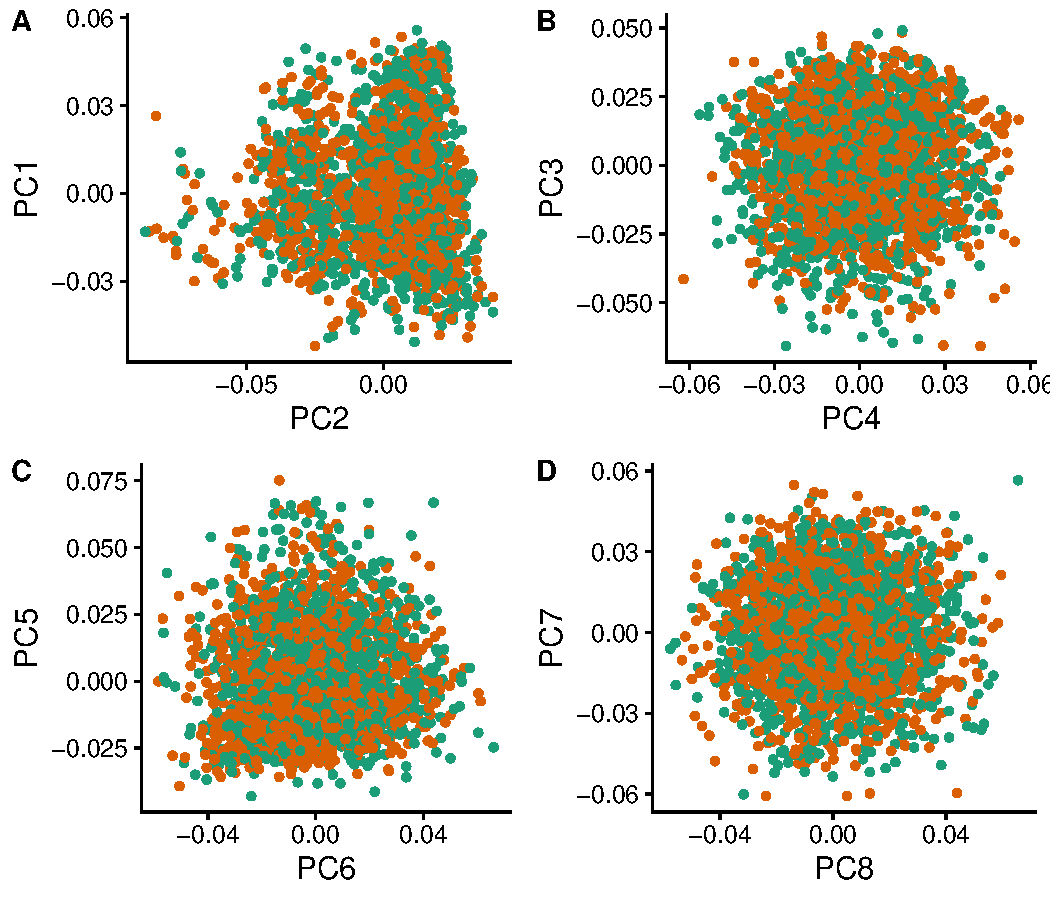
\includegraphics{fig/sfigure_1.pdf}
\caption{\label{fig:pcs}GENESIS shows no differential population structure between cases and controls. \textbf{(A,B,C,D)} Eight main principal components computed on the genotypes of GENESIS. Cases are colored in green, controls in orange.}
\end{figure}

\hypertarget{sec:org6ced6c9}{%
\subsection{High-score subnetwork search algorithms}\label{sec:org6ced6c9}}

\hypertarget{methods:node-score}{%
\subsubsection{SNP and gene association}\label{methods:node-score}}

To measure association between a genotype and the phenotype, we
performed a per-SNP 1 d.f. \(\chi\)\textsuperscript{2} allelic test using PLINK v1.90
(Chang et al. \protect\hyperlink{ref-chang_second-generation_2015}{2015}). Then, we used VEGAS2v2 to compute the
gene-level association score from the SNP P-values (Mishra and Macgregor \protect\hyperlink{ref-mishra_vegas2:_2015}{2015}).
In order to map SNPs to genes we used their overlap on the
genome: all SNPs located within the boundaries of a gene, \(\pm 50\) kb, were
mapped to that gene. To compute the gene association we used the 10\% of
SNPs linked to the gene with lowest P-values. We used the 62,193 genes
described in GENCODE 31 (Frankish et al. \protect\hyperlink{ref-frankish_gencode_2019}{2019}), although only 54,612
could be mapped to at least one SNP. Out of those, we focused
exclusively on the 32,767 that could be mapped to an HGNC symbol. Out of
the SNPs 197,083 remaining after quality control, 164,037 mapped to at
least one of these genes.

We use such mapping to compare the outputs of methods that produce SNP-
to those that produce gene-lists, and vice versa. In the former case, we
consider any gene that can be mapped to any of the selected SNPs as
selected as well. In the latter, we consider all the SNPs that can be
mapped to that gene as selected by the method.

\hypertarget{methods:notation}{%
\subsubsection{Mathematical notation}\label{methods:notation}}

In this chapter, we use undirected, vertex-weighted networks, or graphs,
\(G = (V,E,w)\). \(V = \{v_{1}, \dots{}, v_{n}\}\) refers to the vertices,
with weights \(w: V \rightarrow \mathbb{R}\). Equivalently,
\(E \subseteq \{\{x,y\} | x,y \in V \wedge x \neq y\}\) refers to the
edges. When referring to a subnetwork S, \(V_{S}\) is the set of nodes in
S and \(E_{S}\) is the set of edges in S. A special case of subgraphs are
\emph{connected} subgraphs, which occur when every node in the subgraph can
be reached from any other node.

On top of a weight, nodes have other properties provided by the topology
of the graph. In this chapter we focus on two: degree centrality, and
betweenness centrality. The degree centrality, or degree, is the number
of edges that a node has. The betweenness centrality, or betweenness, is
the number of times a node participates in the shortest paths between
two other nodes.

In addition, we use several matrices that describe different properties
of a graph. The described matrices are square, and have as many rows and
columns as nodes are in the network. The element \((i,j)\) represents a
selected relationship between \(v_i\) and \(v_j\). The \emph{adjacency matrix}
\(W_G\) contains a 1 when the corresponding nodes are connected through an
edge, and 0 otherwise; the diagonal is zero. The \emph{degree matrix} \(D_G\)
is a diagonal matrix which contains the degree of the different nodes.
Lastly, the \emph{Laplacian matrix} \(L_G\) is defined as \(L_G = D_G - W_G\).

\hypertarget{methods:methods}{%
\subsubsection{Methods used}\label{methods:methods}}

Beyond the assumption that genes that contribute to the same function
will be nearby in the protein-protein interaction network (PPIN), they
might be topologically related to each other in diverse ways (densely
interconnected modules, nodes around a hub, a path, etc.). That is not
the only choice to make: how to score the nodes, whether the affected
mechanisms form a single connected component or several, how to frame
the problem in a computationally efficient fashion, what is the best
network to use, etc. In consequence, multiple solutions have been
proposed. In this chapter, we examine six of them: five that explore the
protein-protein interaction network, and one which explores SNP
networks. We selected methods that were open source, had an
implementation available, and an accessible documentation. Their main
differences are summarized in Table \ref{tab:method-comparison}.



















\begin{table}

\caption{\label{tab:method-comparison}Summary statistics on the results of multiple network methods on the gene-gene interaction network. The first row contains the summary statistics on the whole network.}
\centering
\resizebox{\linewidth}{!}{
\begin{threeparttable}
\begin{tabular}[t]{lllllllll}
\toprule
Method & Field & Nodes & Exhaustive & Solution & Components & Input & Scoring & Reference\\
\midrule
\rowcolor{gray!6}  dmGWAS & GWAS & Genes & No &  & 1 & Summary & -log\textsubscript{10}(P) & Jia et al. (\protect\hyperlink{ref-jia_dmgwas:_2011}{2011})\\
heinz & Omics & Genes & Yes &  & 1 & Summary & BUM & M. Dittrich et al. (\protect\hyperlink{ref-dittrich_identifying_2008}{2008})\\
\rowcolor{gray!6}  HotNet2 & Omics & Genes & Yes & Modular & > 1 & Summary & Local FDR & Leiserson et al. (\protect\hyperlink{ref-leiserson_pan-cancer_2015}{2015})\\
LEAN & Omics & Genes & Yes & Star & > 1 & Summary & -log\textsubscript{10}(P) & Gwinner et al. (\protect\hyperlink{ref-gwinner_network-based_2016}{2016})\\
\rowcolor{gray!6}  SConES & GWAS & SNPs & Yes & Modular & > 1 & Genotypes & \(\chi^2\) & Azencott et al. (\protect\hyperlink{ref-azencott_efficient_2013}{2013})\\
\addlinespace
SigMod & GWAS & Genes & Yes & Modular & 1 & Summary & -log\textsubscript{10}(P) & Liu et al. (\protect\hyperlink{ref-liu_sigmod:_2017}{2017})\\
\bottomrule
\end{tabular}
\begin{tablenotes}
\small
\item \textit{Note: } 
\item \emph{Field}: field in which the algorithm was developed. \emph{Nodes}, the type of network, either gene (protein-protein interaction network usually) or a SNP network. \emph{Exhaustive}: whether all the possible solutions given the selected hyperparameters are explored. \emph{Solution}: additional properties are enforced on the solution subnetwork, other than being dense in high scores and connected. \emph{Components}: number of connected subnetworks in the solution. \emph{Input}: genotype data or GWAS summary statistics. \emph{Scoring}: how SNP/gene P-values are transformed into node scores.
\end{tablenotes}
\end{threeparttable}}
\end{table}

\begin{description}
\item[dmGWAS]
dmGWAS searches the subgraph with the highest local density in low
P-values (Jia et al. \protect\hyperlink{ref-jia_dmgwas:_2011}{2011}). To that end it searches candidate
subnetwork solutions using a greedy, ``seed and extend'', heuristic:

\begin{enumerate}
\def\labelenumi{\arabic{enumi}.}
\item
  Select a seed node.
\item
  Compute Stouffer's Z-score Z\textsubscript{m} for the current subgraph as

  \[Z_m = \frac{\sum z_i}{\sqrt{k}}\]

  where \emph{k} is the number of genes in the subgraph, z\textsubscript{i} =
  \(\phi\)\textsuperscript{-1}(1 - P-value\textsubscript{i}), and \(\phi\)\textsuperscript{-1} is the inverse normal
  distribution function.
\item
  Identify neighboring nodes i.e.~nodes at distance \(\le\) \emph{d}. We
  set d = 2.
\item
  Add the neighboring nodes whose inclusion increases the Z\textsubscript{m+1}
  more than Z\textsubscript{m} (1 + r). In our experiments, we set r = 0.1.
\item
  Repeat 2-4 until no increment Z\textsubscript{m} (1 + r) is possible.
\end{enumerate}

Lastly, the module's Z-score is normalized as

\[Z_{N}=\frac{Z_{m}-\operatorname{mean}\left(Z_{m}(\pi)\right)}{\operatorname{SD}\left(Z_{m}(\pi)\right)}\]

where Z\textsubscript{m}(\(\pi\)) represent a vector containing 100000 random
subsets of the same number of genes.

We used the implementation of dmGWAS in the dmGWAS 3.0 R package
(Wang and Jia \protect\hyperlink{ref-dmgwas}{2014}). We used the function \emph{simpleChoose} to select the
solution subnetwork, which aggregates the top 1\% modules into the
solution subnetwork.
\item[heinz]
The goal of heinz is to identify the highest-scored connected
subgraph on the network (M. Dittrich et al. \protect\hyperlink{ref-dittrich_identifying_2008}{2008}). The authors
propose a transformation of the genes' P-value into a score that is
negative under no association with the phenotype, and positive value
when there is. This transformation is achieved by modelling the
distribution of P-values by a beta-uniform model (BUM) parameterized
by the desired FDR. Thus formulated, the problem is NP-complete. To
solve it efficiently it is re-casted as the Prize-Collecting Steiner
Tree Problem (PCST), which seeks to select the connected subnetwork
S that maximizes the \emph{profit} p(S):

\[p(S) = \sum_{v \in V_S} p(v) - \sum_{e \in E_S} c(e).\]

were p(v) = w(v) - w' is the \emph{profit} of adding a node, c(e) = w' is
the \emph{cost} of adding an edge, and \(w' = min_{v \in V_{G}} w(v)\). All
three are positive quantities. heinz implements the algorithm from
Ljubić et al. (\protect\hyperlink{ref-ljubic_algorithmic_2006}{2006}), which in practice is often fast and
optimal, neither is guaranteed. We used BioNet's implementation of
heinz, available on Bioconductor (Beisser et al. \protect\hyperlink{ref-beisser_bionet:_2010}{2010}; M. Dittrich and Beisser \protect\hyperlink{ref-heinz}{2008}).
\item[HotNet2]
HotNet2 was developed to find connected subgraphs of genes
frequently mutated in cancer (Leiserson et al. \protect\hyperlink{ref-leiserson_pan-cancer_2015}{2015}). To that
end, it considers both the local topology of the network and the
scores of the nodes. The former is captured by an insulated heat
diffusion process: at the beginning, the score of the node
determines its initial heat; iteratively each node yields heat to
its ``colder'' neighbors, and receives heat from its ``hotter''
neighbors, while retaining part of its own (hence, \emph{insulated}).
This process continues until equilibrium is reached, and results in
a similarity matrix F. F is used to compute the similarity matrix E
that accounts also for similarities in node scores as

\[E = F \operatorname{diag}(w(V)),\]

where \(\operatorname{diag}(w(V))\) is a diagonal matrix with the node
scores in its diagonal. We scored the nodes as in
Nakka, Raphael, and Ramachandran (\protect\hyperlink{ref-nakka_gene_2016}{2016}), assigning a score of 0 for the genes with low
probability of being associated to the disease, and
-log\textsubscript{10}(P-value) to those likely to be. In this dataset, the
threshold separating both was a P-value of 0.125, which was obtained
using a local FDR approach (Scheid and Spang \protect\hyperlink{ref-scheid_twilight_2005}{2005}). To obtain
densely connected subnetworks, HotNet2 prunes E, only preserving
edges such that w(E) \textgreater{} \(\delta\). Lastly, HotNet2 evaluates the
statistical significance of the subnetworks by comparing their size
to the size of networks obtained by permuting the node scores.
HotNet2 has two parameters: the restart probability \(\beta\), and the
threshold heat \(\delta\). Both parameters are set automatically by
the algorithm, and are robust (Leiserson et al. \protect\hyperlink{ref-leiserson_pan-cancer_2015}{2015}). HotNet2
is implemented in Python (Leiserson et al. \protect\hyperlink{ref-hotnet2}{2018}).
\item[LEAN]
LEAN searches disregulated ``star'' gene subnetworks, that is,
subnetworks composed by one central node and all its interactors
(Gwinner et al. \protect\hyperlink{ref-gwinner_network-based_2016}{2016}). By imposing this restriction, LEAN is
able to exhaustively test all such subnetworks (one per node). For a
particular subnetwork of size \emph{m}, the P-values corresponding to the
involved nodes are ranked as p\textsubscript{1} \(\le\) \ldots{} \(\le\) p\textsubscript{m}. Then, \emph{k}
binomial tests are conducted, to compute the probability of having
\emph{k} out of \emph{m} P-values lower or equal to p\textsubscript{k} under the null
hypothesis. The minimum of these \emph{k} P-values is the score of the
subnetwork. This score is transformed into a P-value through an
empirical distribution obtained via a subsampling scheme, where sets
of \emph{m} genes are selected randomly, and their score computed.
Lastly, P-values are corrected for multiple testing through a
Benjamini-Hochberg correction. We used the implementation of LEAN
from the LEANR R package (Gwinner \protect\hyperlink{ref-leanr}{2016}).
\item[SConES]
SConES searches the minimal, modular, and maximally associated
subnetwork in a SNP graph (Azencott et al. \protect\hyperlink{ref-azencott_efficient_2013}{2013}). Specifically,
it solves the problem

\begin{equation}
\underset{S \subseteq G}{\arg \max } \underbrace{\sum_{v \in V_S} w(v)}_{\text { association }} + \underbrace{\lambda \sum_{v \in V_S} \sum_{u \not\in V_S} L_{vu} }_{\text { connectivity }}-\underbrace{\eta \lvert V_S \rvert }_{\text { sparsity }}
\label{eq:scones}
\end{equation}

where \(\lambda\) and \(\eta\) are hyperparameters that control the
sparsity and the connectivity of the model. Given two
hyperparameters, the aforementioned problem has a unique solution,
that SConES finds using a graph min-cut procedure. We used the
version on SConES implemented in the R package martini (Climente-González and Azencott \protect\hyperlink{ref-martini}{2019}).
As in Azencott et al. (\protect\hyperlink{ref-azencott_efficient_2013}{2013}), we selected \(\lambda\) and \(\eta\)
by cross-validation, choosing the values that produce the most
stable solution across folds. Note that the solution to the above
problem can consist of several connected subnetworks which are
disconnected from each other. In this case, the selected
hyperparameters were \(\eta\) = 3.51, \(\lambda\) = 210.29 for SConES
GS; \(\eta\) = 3.51, \(\lambda\) = 97.61 for SConES GM; and \(\eta\) =
3.51, \(\lambda\) = 45.31 for SConES GI.
\item[SigMod]
SigMod aims at identifying the most densely connected gene
subnetwork that is most strongly associated to the phenotype
(Liu et al. \protect\hyperlink{ref-liu_sigmod:_2017}{2017}). It addresses an optimization problem similar to
that of SConES (Equation \eqref{eq:scones}), but using the adjacency
matrix rather than the Laplacian matrix (Section \ref{methods:notation}),
to quantify solutions containing many edges.

\[\underset{S \in G}{\arg \max } \underbrace{\sum_{v \in V_S} w(v)}_{\text { association }} + \underbrace{\lambda \sum_{v \in V_S} \sum_{u \in V_S} W_{vu} }_{\text { connectivity }} -\underbrace{\eta \lvert V_S \rvert }_{\text { sparsity }}.\]

As SConES, this optimization problem can also be solved by a graph
min-cut approach.

SigMod presents three important differences with SConES. First it is
designed for gene-gene networks. Second, by replacing the adjacency
by the Laplacian matrix, it favors subnetworks containing many
edges. SConES, instead, penalizes connections between the
selected and unselected nodes. Third, it returns a single connected
subnetwork, which it achieves by exploring a grid of hyperparameters
and processing their respective solutions. Specifically, for the
range of \(\lambda\) = \(\lambda\)\textsubscript{min}, \ldots, \(\lambda\)\textsubscript{max} for the
same \(\eta\), it prioritizes the solution with the largest change in
size from \(\lambda\)\textsubscript{n} to \(\lambda\)\textsubscript{n+1}. Such a large change
implies that the network is strongly interconnected. This results in
one candidate solution for each \(\eta\), which are processed by
removing any node not connected to any other. A score is assigned to
each candidate solution by summing their node scores and normalizing
by size. The candidate solution with the highest standardized score
is the chosen solution. SigMod is implemented in an R package
(Y. Liu \protect\hyperlink{ref-sigmod}{2018}).
\end{description}

\hypertarget{methods:gene-network}{%
\subsubsection{Gene-gene network}\label{methods:gene-network}}

Out of the six methods tested, five use a gene-gene interaction network
(Section \ref{methods:methods}). Although their respective statistical
frameworks are compatible with any type of network (protein
interactions, gene coexpression, regulatory, etc.), for practical
reasons we focused on a PPIN, as they are interpretable, well
characterized, and most of the methods were designed to scale
appropriately to it. We built our PPIN from both binary and co-complex
interactions stored in the HINT database (release April 2019)
(Das and Yu \protect\hyperlink{ref-das_hint_2012}{2012}). Unless specified otherwise, we used only interactions
coming from high-throughput experiments to avoid biasing the topology of
the network by well-studied genes with more known interactions on
average. Out of the 146,722 interactions from high-throughput
experiments that HINT stores, we were able to map 142,541 to a pair of
HGNC symbols. The scoring function for the nodes changed from method to
method (Section \ref{methods:methods}).

Additionally, we compared the results of the aforementioned PPIN with
those obtained on another PPIN built using interactions coming from both
high-throughput and targeted studies. In that case, out of the 179,332
interactions in HINT, we mapped 173,797 to a pair of HGNC symbols.

\hypertarget{methods:snp-network}{%
\subsubsection{SNP networks}\label{methods:snp-network}}

SConES (Azencott et al. \protect\hyperlink{ref-azencott_efficient_2013}{2013}) is the only of the studied methods
designed to handle SNP networks. As in gene networks, two SNPs are
linked in a SNP network when there is evidence of shared functionality
between two SNPs. The authors suggested three ways of building these
networks: connecting the SNPs consecutive in the genomic sequence (``GS
network''); interconnecting all the SNPs mapped to the same gene, on top
of GS (``GM network''); and interconnecting all SNPs mapped to two genes
for which a protein-protein interaction exists (``GI network''). We
focused on the GI network, as it is the network that fits better the
scope of this chapter. However, at different stages of the chapter we
also used GS and GM. For the GM network, we used the mapping described
in Section \ref{methods:node-score}. For the GI network, we used the PPI as
described in Section \ref{methods:gene-network}. For all three networks the
node score used is the association of the individual SNPs with the phenotype;
specifically, we used the 1 d.f. \(\chi\)\textsuperscript{2}.

\hypertarget{methods:consensus}{%
\subsubsection{Consensus network}\label{methods:consensus}}

The different high-weight subnetwork discovery algorithms make different
assumptions on the properties of the solutions, and employ different
strategies to find them. Hence, combining the outcome of the different
approaches might provide a more complete outlook on the specific
alterations on the GENESIS dataset. We built such consensus network by
retaining the nodes that were selected by at least two of the methods.
We combined the results of 6 methods: dmGWAS, heinz, HotNet2, LEAN,
SConES GI, and SigMod.

\hypertarget{sec:orgc968928}{%
\subsection{Evaluation of methods}\label{sec:orgc968928}}

\hypertarget{methods:comparison}{%
\subsubsection{Classification accuracy of selected biomarkers}\label{methods:comparison}}

A desirable solution is one that is sparse, while offering a good
predictive power on unseen samples. We evaluated the predicting power of
the SNPs selected by the different methods through the performance of an
L1-penalized logistic regression trained exclusively on those SNPs to
predict the outcome (case/control). The L1 penalty helps to account for
LD to reduce the number of SNPs included in the model (size of the
active set), while improving the generalization of the classifier. The
value of the regularization parameter, which controls both the magnitude
and the sparsity of the coefficients, was set by cross-validation. To
that end, we used the different network-methods on a random subset of
80\% of the samples. On this same subset we trained our classifier
exclusively on the SNPs selected by a particular method. When the method
retrieved a list of genes (all of them except SConES), all the SNPs
mapped to any of those genes were used. Then we
evaluated performance of the classifier on the remaining 20\% of the
dataset. We repeated this procedure 5 times to estimate the average and
the deviation of the different performance measures. The
performance measures we used were: size of the solution, size of the
active set, specificity, and sensitivity. The size of the active set
provides an estimate of a plausible, more sparse solution with a
comparable predictive power to the original solution.

Additionally, for each of the methods, we evaluated their stability and
their runtime. The stability of an algorithm is its sensitivity to small
changes of the input, and is measured using the Pearson's correlation
between different runs as suggested in Nogueira and Brown (\protect\hyperlink{ref-nogueira_measuring_2016}{2016}). To
obtain a baseline, we also performed the procedure using all the SNPs.
Lastly, another desirable property is that the method retrieves a good
candidate causal subnetwork. In consequence, we compared the outcome of
each of the methods to the consensus subnetwork of all the solutions
(Section \ref{methods:consensus}).

\hypertarget{methods:bcac}{%
\subsubsection{Biological relevance of the genes}\label{methods:bcac}}

An alternative way to validate the results is comparing our results to
an external dataset. For that purpose, we recovered a list of 153 genes
associated to familial breast cancer from DisGeNET
(Piñero et al. \protect\hyperlink{ref-pinero_disgenet:_2017}{2017}). Across this chapter we refer to these genes as
\emph{breast cancer susceptibility genes}.

Additionally, we used the summary statistics from the Breast Cancer
Association Consortium (BCAC) (Michailidou et al. \protect\hyperlink{ref-michailidou_genome-wide_2015}{2015}). BCAC has
conducted one of the largest efforts in GWAS, involving over 120,000
women of European ancestry. As opposed to GENESIS, samples were not
selected based on family history, and hence the study is enriched in sporadic
breast cancers. Another difference is that BCAC is a relatively
heterogeneous study on a pan-European sample, while GENESIS is a
homogeneous dataset focused on the French population. Despite these
differences, there should be shared genetic architecture. On top of
that, that overlap should become larger when the results are aggregated
at the gene level. For that purpose, we computed the gene association as
in Section \ref{methods:node-score}. The iCOGS array was used for genotyping in
BCAC (Sakoda, Jorgenson, and Witte \protect\hyperlink{ref-sakoda_turning_2013}{2013}), the same array as for GENESIS
(Sinilnikova et al. \protect\hyperlink{ref-sinilnikova_genesis:_2016}{2016}). Although imputed data are available, we
used exclusively the SNPs available on GENESIS after quality control to
make the results comparable.

\hypertarget{sec:org1d907c0}{%
\subsection{Code availability}\label{sec:org1d907c0}}

This work required developing computational pipelines for several GWAS
analyses, such physically mapping SNPs to genes, computing gene scores,
and performing six different network analyses. For each of those
processes, a streamlined, project-agnostic pipeline with a clear
interface was created. They are compiled in the following GitHub
repository: \url{https://github.com/hclimente/gwas-tools}. The code that
applies these pipelines to the GENESIS project, as well as the code that
reproduces all the analyses in this chapter are available at
\url{https://github.com/hclimente/genewa}. Although the GENESIS dataset is
not publicly available, the published code should work on any other GWAS
dataset. All the produced gene subnetworks were deposited on NDEx
(\url{http://www.ndexbio.org}), under the UUID
e9b0e22a-e9b0-11e9-bb65-0ac135e8bacf.

\hypertarget{sec:orgc718f04}{%
\section{Results}\label{sec:orgc718f04}}

\hypertarget{results:conventional}{%
\subsection{A conventional GWAS shows that FGFR2 is strongly associated with familial breast cancer}\label{results:conventional}}



\begin{figure}
\centering
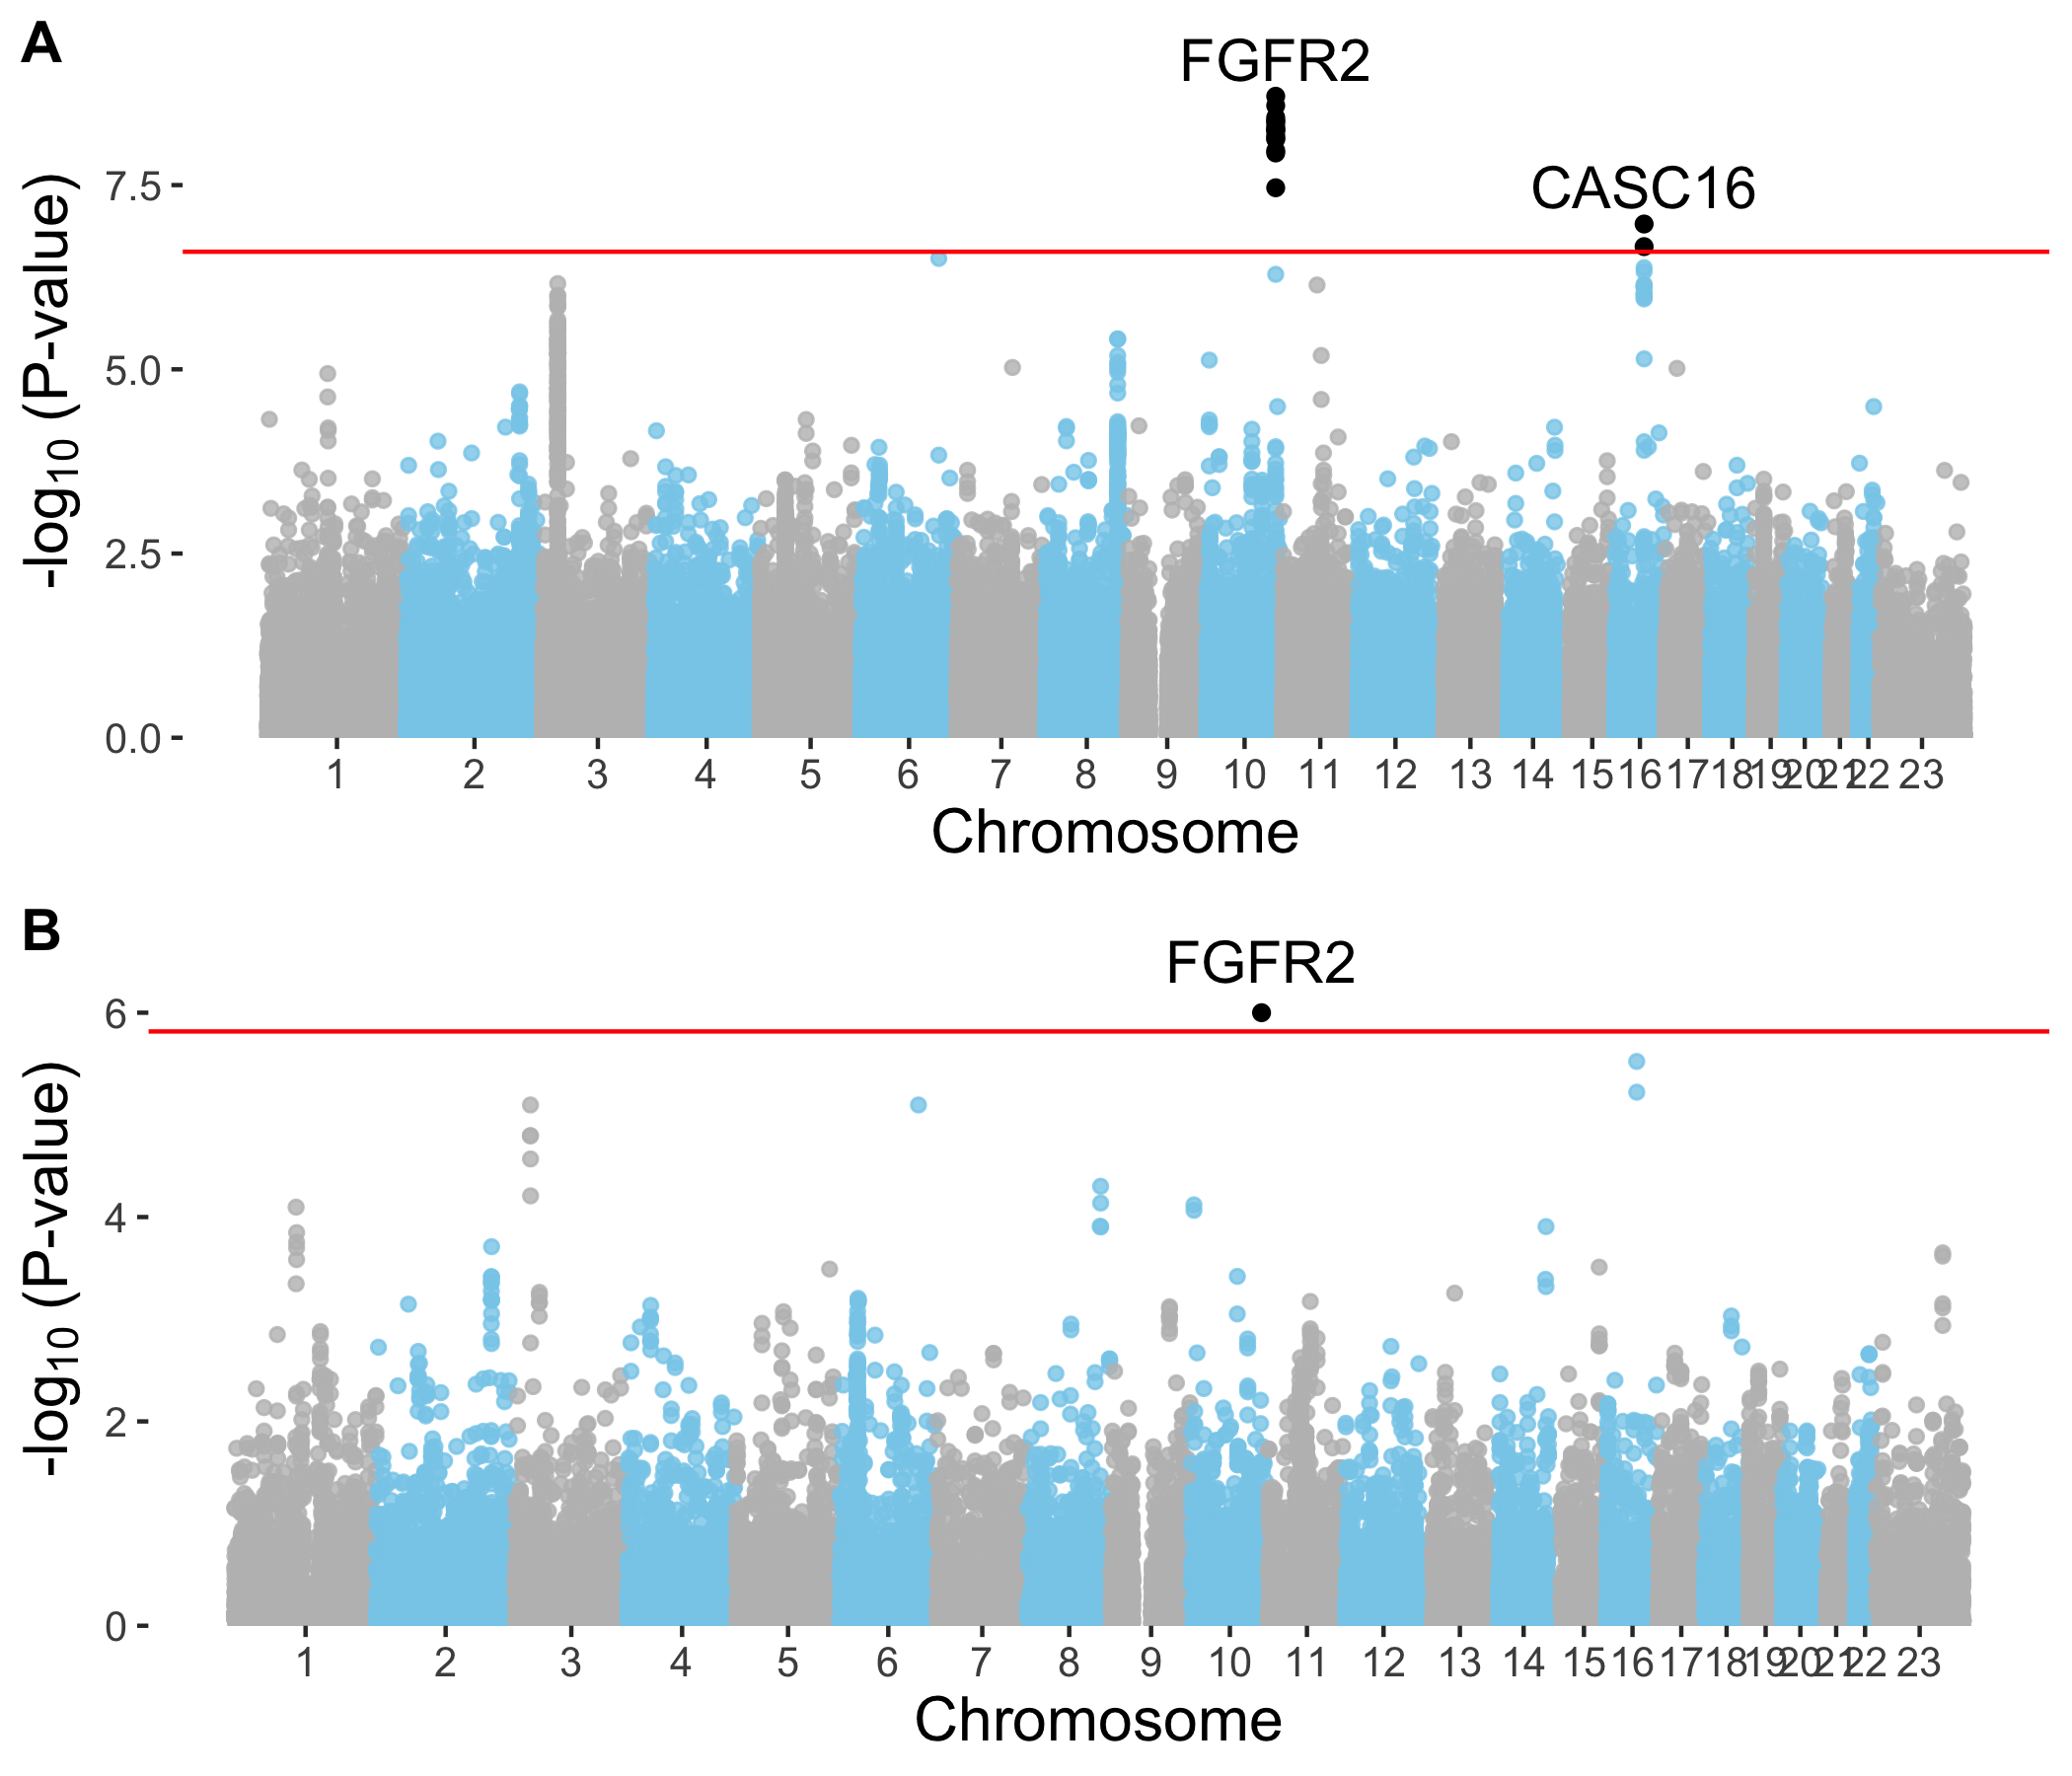
\includegraphics{fig/figure_1.png}
\caption{\label{fig:snp-gene-manhattan}Association in GENESIS. The red line represents the Bonferroni threshold. \textbf{(A)} SNP association, measured from the outcome of a 1df \(\chi^2\) allelic test. Significant SNPs that are within a coding gene, or within 50 kilobases of its boundaries, are annotated. The Bonferroni threshold is \(2.54 \times 10^{-7}\). \textbf{(B)} Gene association, measured by P-value of VEGAS2v2 (Mishra and Macgregor \protect\hyperlink{ref-mishra_vegas2:_2015}{2015}) using the 10\% of SNPs with the lowest P-values. The Bonferroni threshold is \(1.53 \times 10^{-6}\).}
\end{figure}

We conducted association analyses in the GENESIS dataset at both the SNP
and the gene levels (Section \ref{methods:node-score}). Two genomic regions
have a P-value lower than the Bonferroni threshold in chromosomes 10 and 16
(Figure \ref{fig:snp-gene-manhattan} A). The former overlaps with gene
\emph{FGFR2}; the latter with \emph{CASC16}, and it is located near the
protein-coding gene \emph{TOX3}. Variants in both \emph{FGFR2} and \emph{TOX3} were
related to breast cancer susceptibility in other cohorts negative for
\emph{BRCA1/2} (Rinella et al. \protect\hyperlink{ref-rinella_genetic_2013}{2013}). Only the peak in chromosome 10
replicated in the gene-level analysis, with \emph{FGFR2} just above the
threshold of significance (Figure \ref{fig:snp-gene-manhattan}B).

These results show the overlap in the genetic architecture of the
disease between the studied French population sample and other
populations, especially at the gene level. In addition, there are other
SNPs whose P-values, although higher than the conventional threshold of
significance, show a strong association with familial breast cancer. The
most prominent of such regions are 3p24 and 8q24, both of which have
been associated to breast cancer susceptibility in the past
(Brisbin et al. \protect\hyperlink{ref-brisbin_meta-analysis_2011}{2011}; Ahmed et al. \protect\hyperlink{ref-search_newly_2009}{2009}). This motivates
exploring network methods, which trade statistical significance for
biological relevance.

\hypertarget{results:separate-networks}{%
\subsection{Network methods successfully identify genes associated with breast cancer}\label{results:separate-networks}}









\begin{table}

\caption{\label{tab:gene-solutions}Summary statistics on the results of multiple network methods on the gene-gene interaction network. The first row contains the summary statistics on the whole network.}
\centering
\resizebox{\linewidth}{!}{
\begin{threeparttable}
\begin{tabular}[t]{llllll}
\toprule
Network & Num genes & Num edges & \(\overline{\mbox{Betweenness}}\) & \(\hat{\mbox{P}}_{gene}\) & \(\rho_{consensus}\)\\
\midrule
\rowcolor{gray!6}  HINT HT & 13619 & 142541 & 16706 & 0.46 & 0.066\\
Consensus & 55 & 117 & 74062 & 0.0051 & 1\\
\rowcolor{gray!6}  dmGWAS & 194 & 450 & 49115 & 0.19 & 0.41\\
heinz & 4 & 3 & 113633 & 0.0012 & 0.21\\
\rowcolor{gray!6}  HotNet2 & 440 & 374 & 7739 & 0.048 & 0.31\\
\addlinespace
LEAN & 0 & 0 & NA & NA & NA\\
\rowcolor{gray!6}  SConES GI & 0 (1) & 0 & NA & NA & NA\\
SigMod & 142 & 249 & 92603 & 0.0083 & 0.73\\
\bottomrule
\end{tabular}
\begin{tablenotes}
\small
\item \textit{Note: } 
\item \emph{Num genes}: number of genes selected out of those that are part of the PPIN; for SConES GI the total number of genes, including RNA genes, was added in parentheses. \(\overline{\mbox{Betweenness}}\): mean betweenness of the selected genes in the PPIN. \(\hat{\mbox{P}}\)\textsubscript{gene}: median P-value of the selected genes. \(\rho\)\textsubscript{consensus}: Pearson\textbackslash's correlation between the subnetwork and the consensus network.
\end{tablenotes}
\end{threeparttable}}
\end{table}





\begin{table}

\caption{\label{tab:snp-solutions}Summary statistics on the results of SConES on the three SNP-SNP interaction networks. The first row within each block contains the summary statistics on the whole network.}
\centering
\resizebox{\linewidth}{!}{
\begin{threeparttable}
\begin{tabular}[t]{lrlrlr}
\toprule
Network & SNPs & Edges & Subnetworks & \(\overline{\mbox{Betweenness}}\) & \(\hat{\mbox{P}}\)\textsubscript{SNP}\\
\midrule
\rowcolor{gray!6}  GS & 197083 & 1.97e+05 & NA & 2.03e+07 & 0.490\\
SConES GS & 1590 & 1.58e+03 & 5 & 2.52e+07 & 0.023\\
\rowcolor{gray!6}  GM & 197083 & 6.44e+06 & NA & 3.99e+06 & 0.490\\
SConES GM & 1692 & 1.78e+05 & 5 & 4.40e+06 & 0.055\\
\rowcolor{gray!6}  GI & 197083 & 2.87e+07 & NA & 1.46e+06 & 0.490\\
\addlinespace
SConES GI & 408 & 5.39e+02 & 5 & 9.33e+06 & 0.076\\
\bottomrule
\end{tabular}
\begin{tablenotes}
\small
\item \textit{Note: } 
\item \(\overline{\mbox{Betweenness}}\): mean betweenness of the selected SNPs in the corresponding full network; \(\hat{\mbox{P}}\)\textsubscript{SNP}: median P-value of the selected SNPs.
\end{tablenotes}
\end{threeparttable}}
\end{table}

We applied six network methods to the GENESIS dataset (Section
\ref{methods:methods}), obtaining six solutions (Figure
\ref{fig:overview-solutions}): one
for each of the five gene-based methods (Section
\ref{methods:gene-network}), and one for SConES GI (Section
\ref{methods:snp-network}). The solutions are very heterogeneous
(Table \ref{tab:gene-solutions} and Table
\ref{tab:snp-solutions}): none of the subnetworks examined by
LEAN are significant (adjusted P-value \textless{} 0.05), while HotNet2 produced
the largest solution subnetwork with 440 genes. SConES GI failed to
recover genes in the PPIN, but it recovered one genomic region mapped to
RNA gene \emph{RNU6-420P}. All solution subnetworks except LEAN's are, on
average, more strongly associated to breast cancer than the whole PPIN
(median P-values \(\ll 0.46\)), despite containing genes with higher
P-values (Figure \ref{fig:manhattan-solutions}). This exemplifies the
trade-off between statistical significance and biological relevance. However,
there are nuances between solutions: heinz strongly favored highly
associated genes, while dmGWAS is less conservative (median gene
P-values 0.0012 and 0.19, respectively); SConES tended to select whole
LD-blocks; and HotNet2 and SigMod were less likely to select lowly
associated genes.



\begin{figure}
\centering
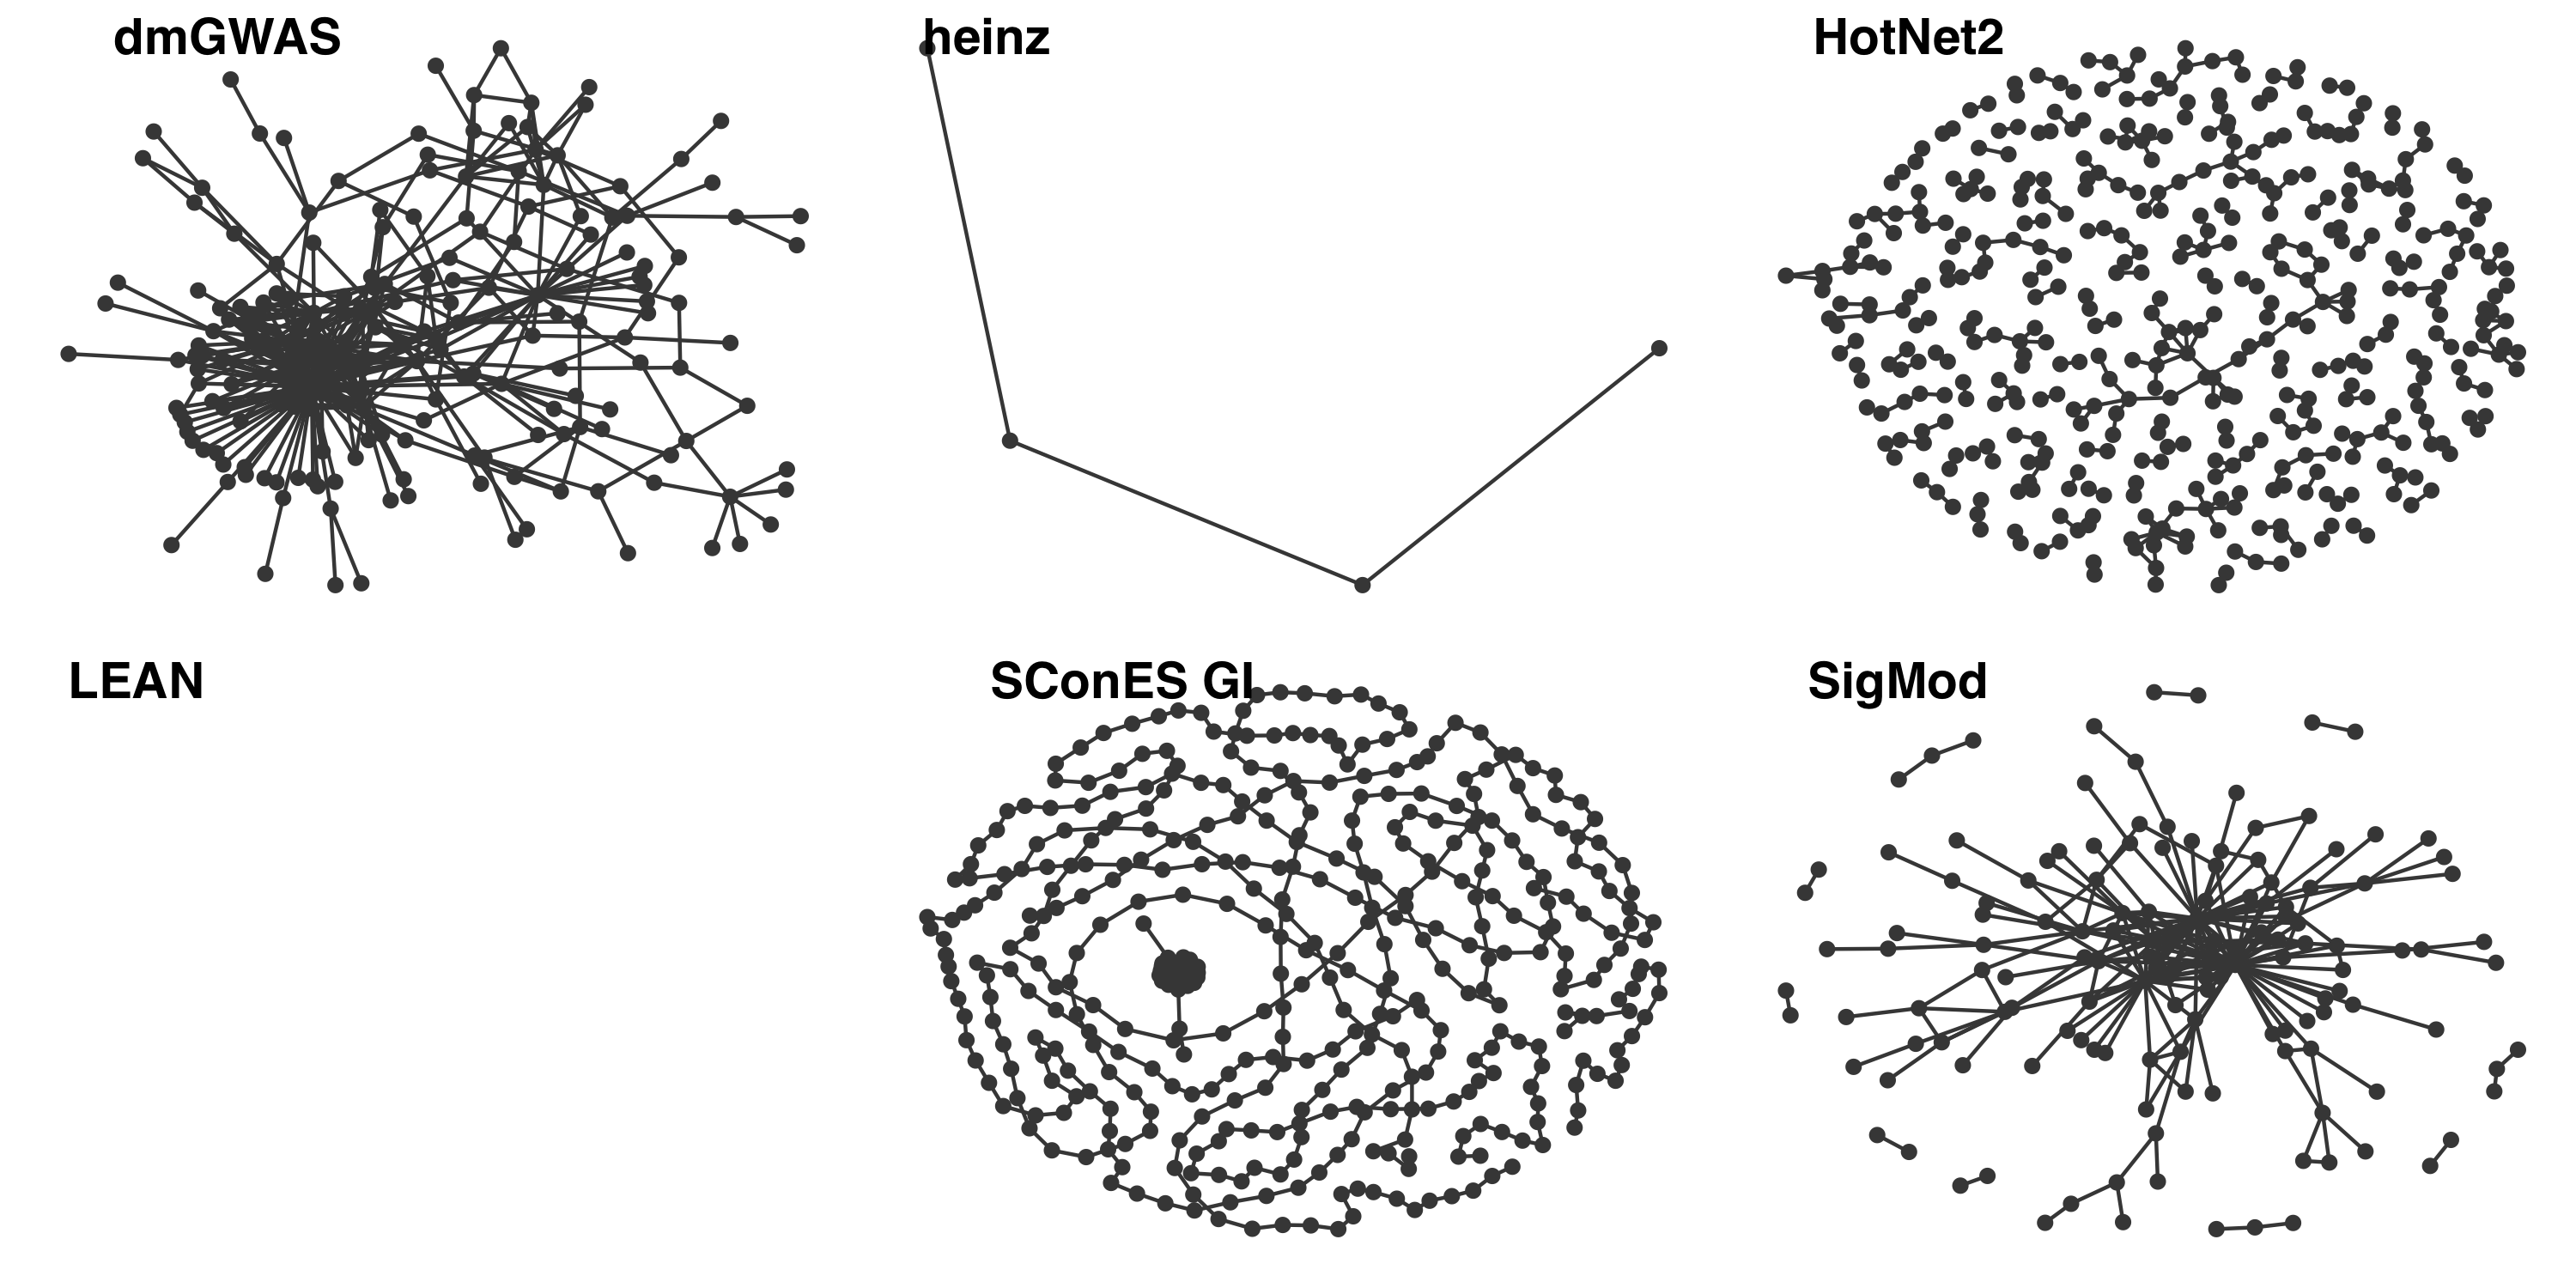
\includegraphics{fig/sfigure_2.png}
\caption{\label{fig:overview-solutions}Overview of the subnetworks produced by the different network methods. \textbf{(dmGWAS, heinz, HotNet2, LEAN, and SigMod)} contain gene subnetworks; \textbf{(SConES GI)}, SNP subnetworks.}
\end{figure}



\begin{figure}

{\centering 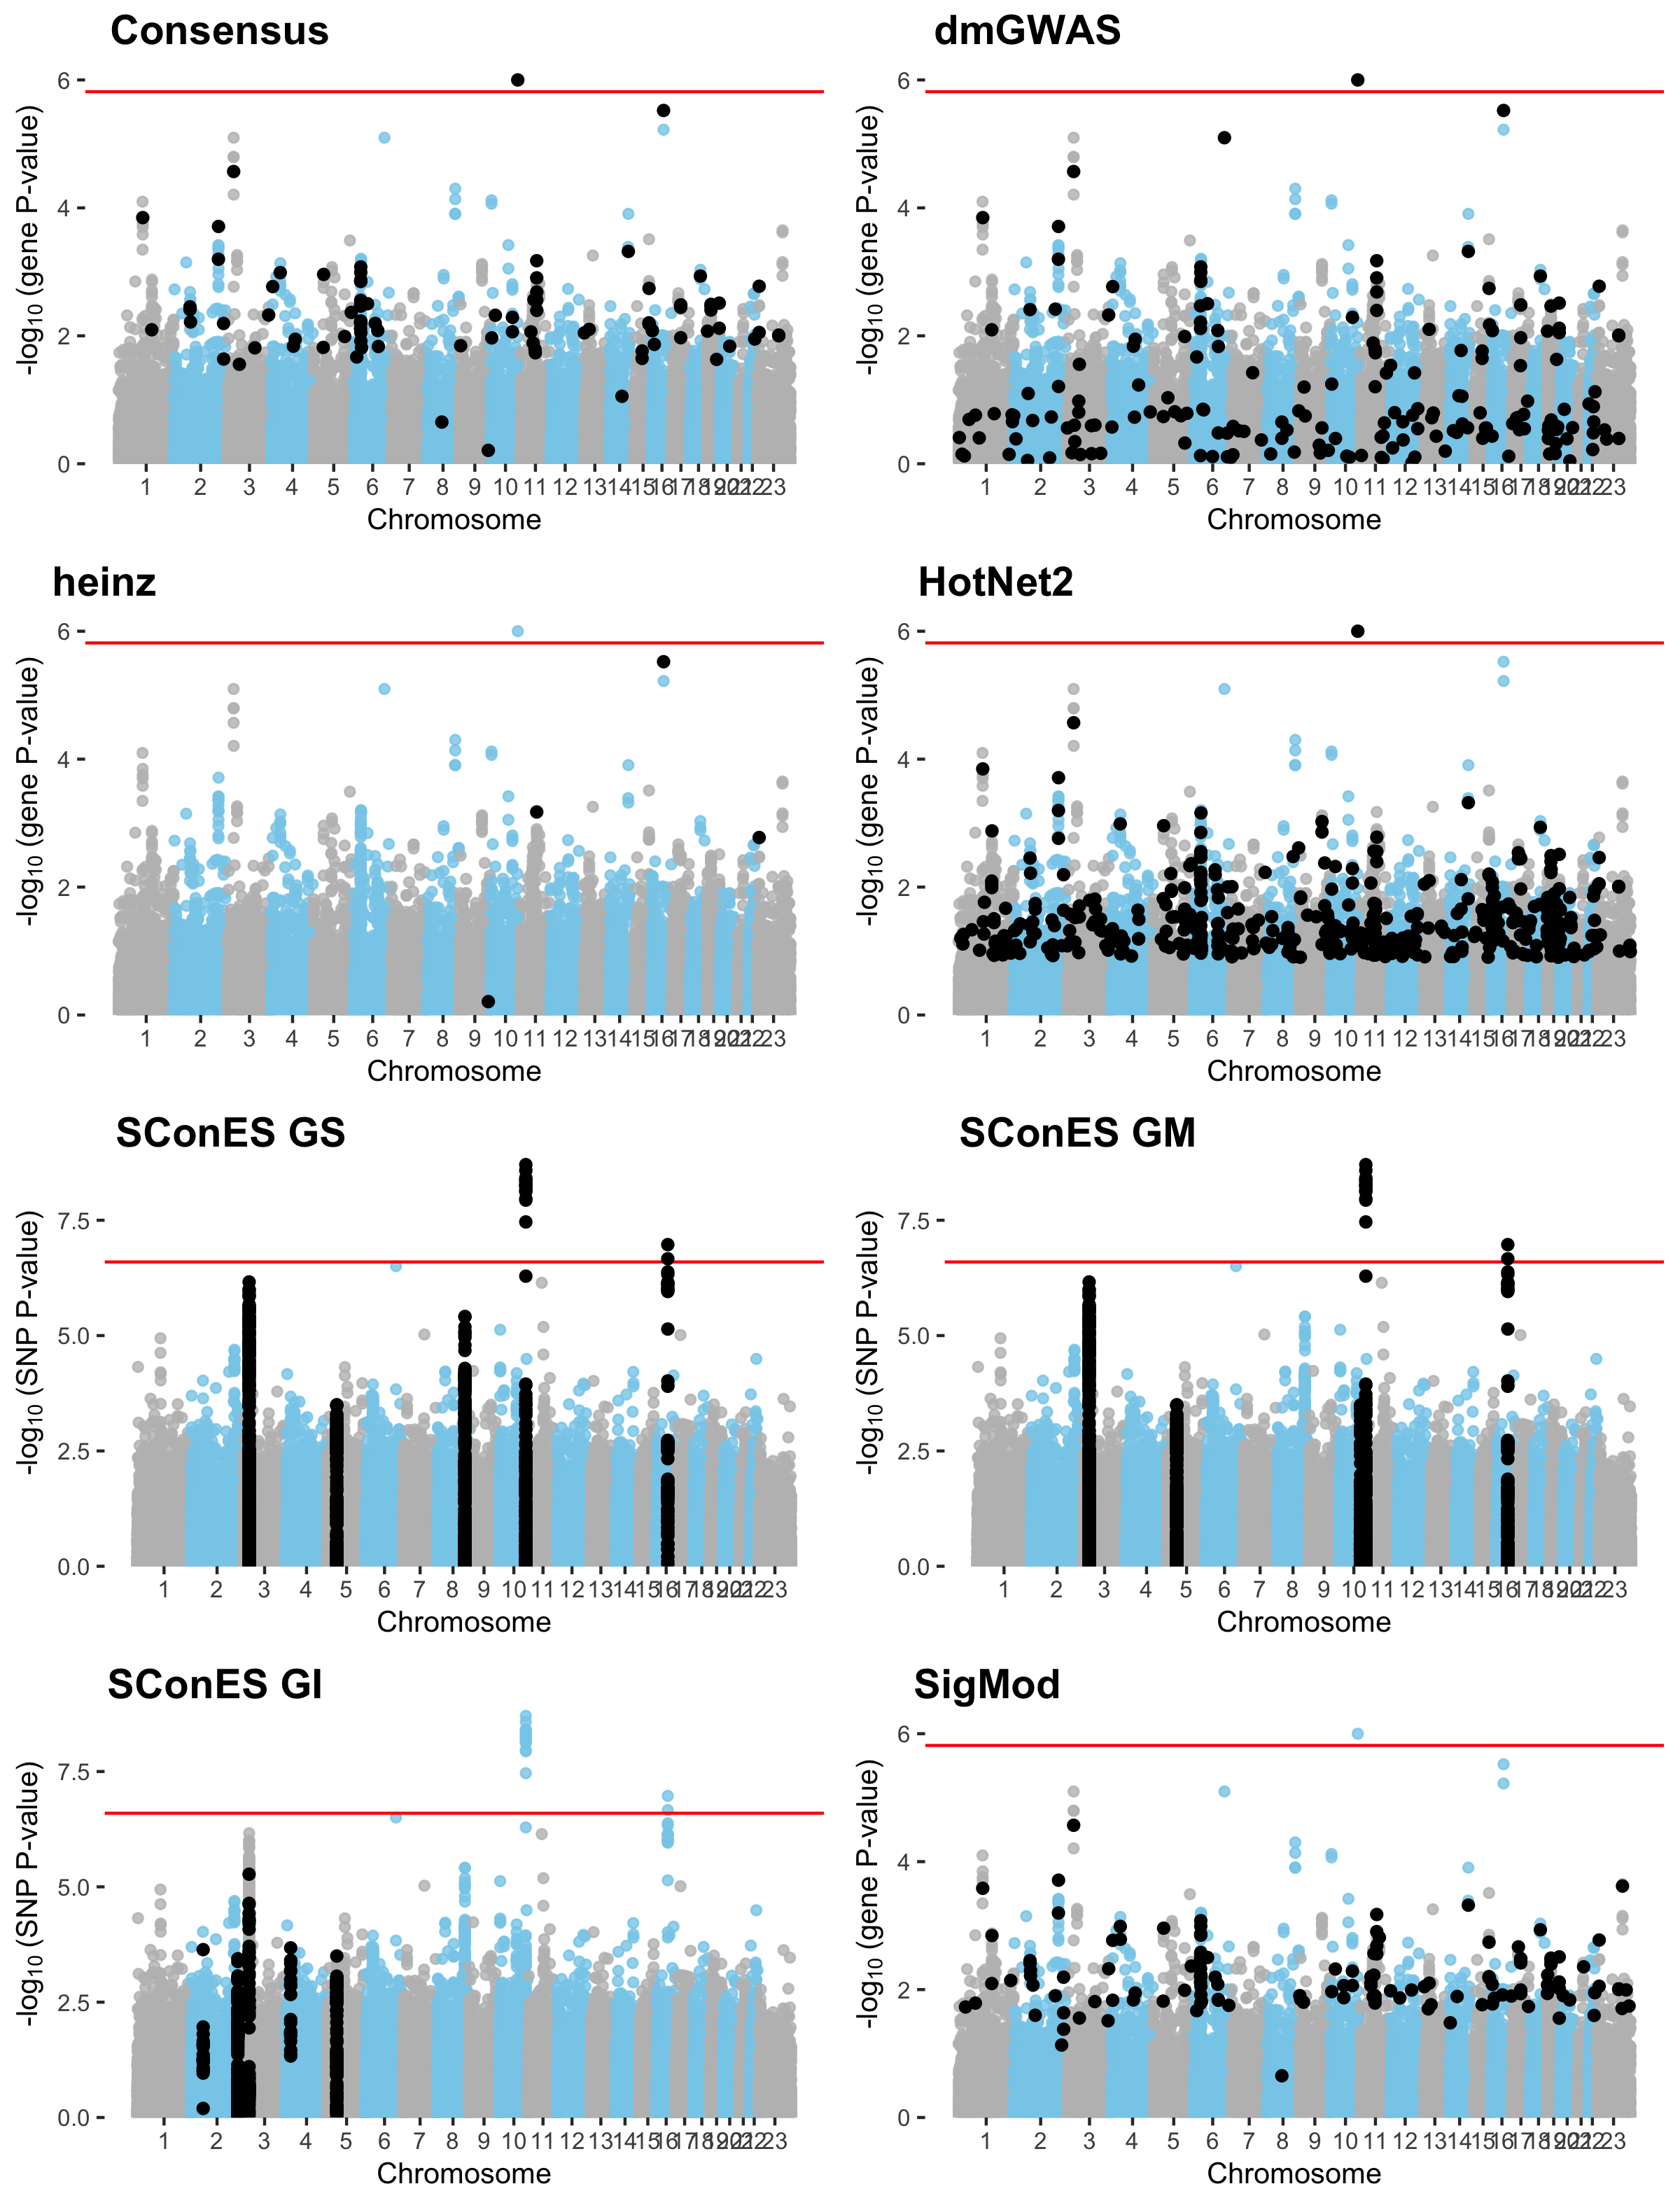
\includegraphics[height=0.8\textheight]{fig/sfigure_3} 

}

\caption{Manhattan plots showing the biomolecules selected by each method. In \textbf{(Consensus, dmGWAS, heinz, HotNet2, and SigMod)} datapoints are genes; in \textbf{(SConES GS, GM, and GI)}, SNPs. LEAN was excluded, as it did not select any gene.}\label{fig:manhattan-solutions}
\end{figure}

The solution subnetworks present other desirable properties. First, four
of the methods succeeded at recovering genes involved in the disease
(Figure \ref{fig:disgenet-comparison}), as their subnetworks were
enriched in breast cancer susceptibility genes (dmGWAS, heinz, HotNet2,
and SigMod, Fisher's exact test one-sided P-value \textless{} 0.03). We also
compared the outcome of the network methods to the association tests
conducted on the population of European ancestry from the Breast Cancer
Association Consortium (BCAC) (Michailidou et al. \protect\hyperlink{ref-michailidou_genome-wide_2015}{2015})
(Figure \ref{fig:bcac-comparison}). Encouragingly, every solution
subnetwork is enriched in genes or SNPs that are Bonferroni-significant
in BCAC. This confirms the capability of network methods to find the
same signal as in more powered studies by leveraging on prior knowledge.
Second, the genes in four solution subnetworks display on average a
higher betweenness centrality than the rest of the genes, a difference
that is significant in three solutions (dmGWAS, and SigMod, Wilcoxon
rank-sum test P-value \textless{} 1.4 10\textsuperscript{-21}). This agrees with the notion that
disease genes are more central than other, non-essential genes
(Piñero et al. \protect\hyperlink{ref-pinero_uncovering_2016}{2016}). We observe that this conclusion holds in this
disease, as known breast cancer susceptibility genes have higher
betweenness centrality than others (one-tailed Wilcoxon rank-sum test
P-value = 2.64 10\textsuperscript{-5}, Figure \ref{fig:consensus-stats}C). Interestingly,
SConES' selected SNPs are also more central than the average SNP (Table
\ref{tab:snp-solutions}), suggesting that causal SNPs are
also more central than unrelated SNPs. However, very central nodes are also
more likely to be connecting a random pair of nodes, making then more
likely to be selected by the examined methods. Hence, further work is
needed draw conclusions.



\begin{figure}

{\centering 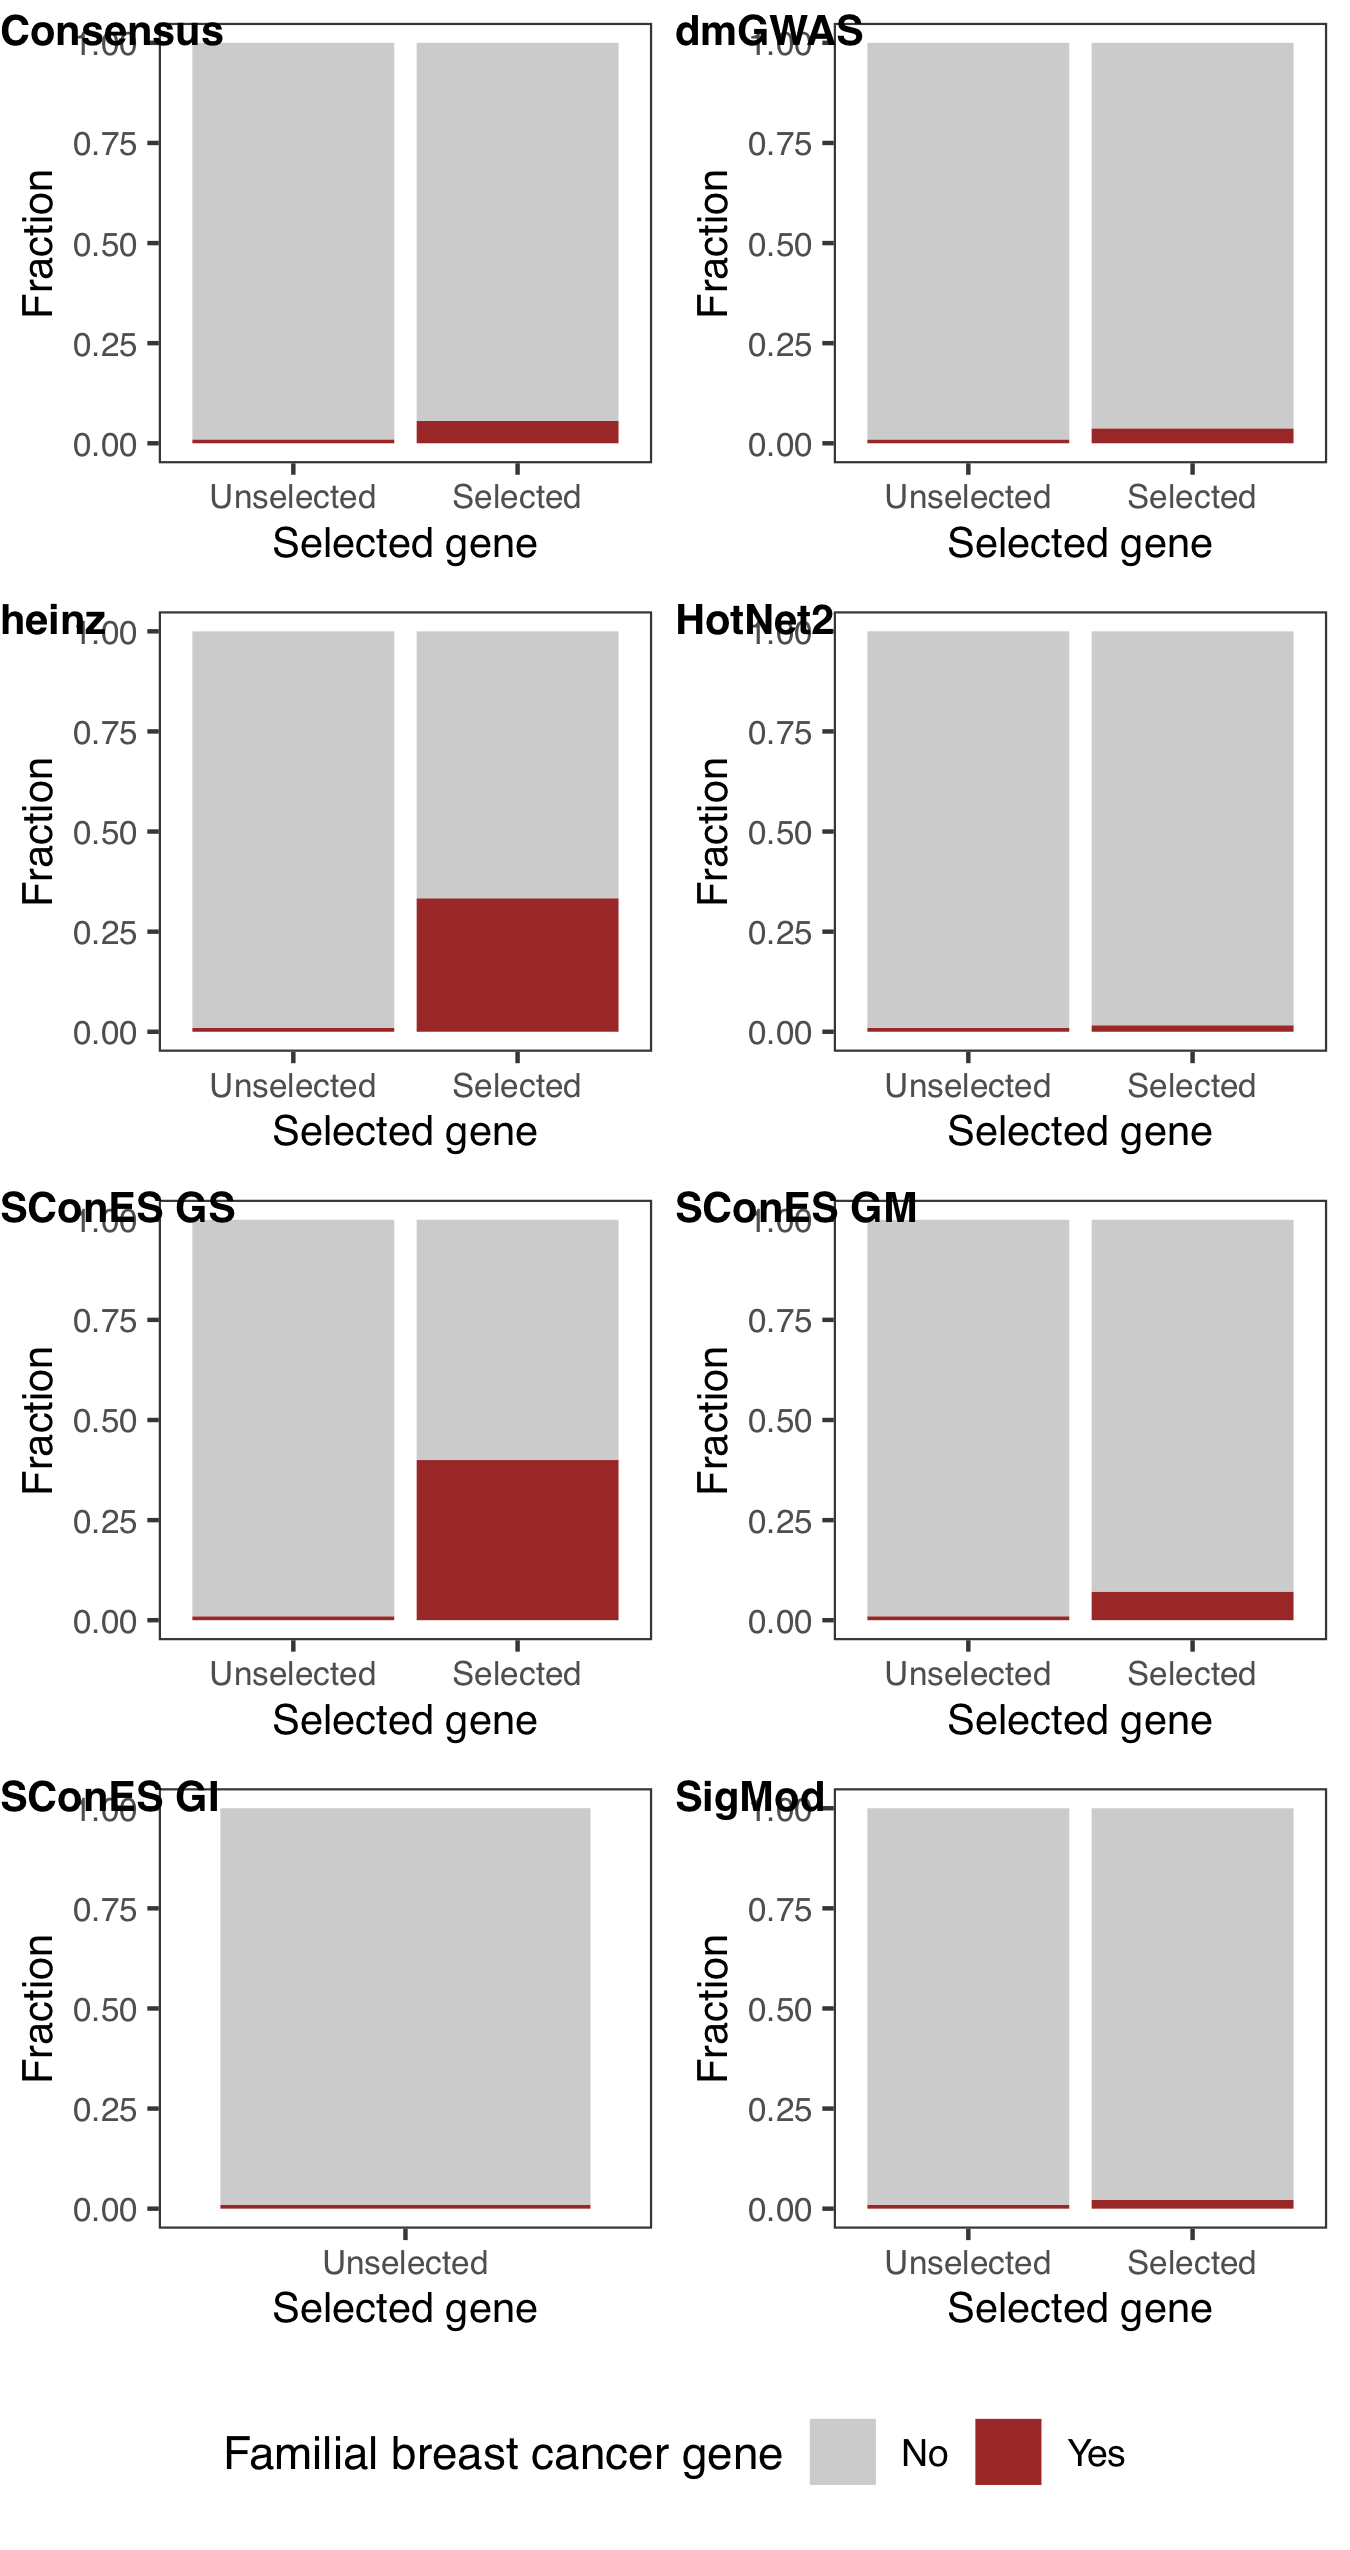
\includegraphics[height=0.8\textheight]{fig/sfigure_5} 

}

\caption{Proportion of the selected genes by each of the methods on the GENESIS data that is a known breast cancer susceptibility gene (Section \ref{methods:bcac}). Only genes present in the protein-protein interaction network were considered. LEAN is not displayed as it did not select any gene. The presented network methods recover a higher proportion of breast cancer susceptibility genes than of other genes, despite their lack of significance in GENESIS.}\label{fig:disgenet-comparison}
\end{figure}



\begin{figure}

{\centering 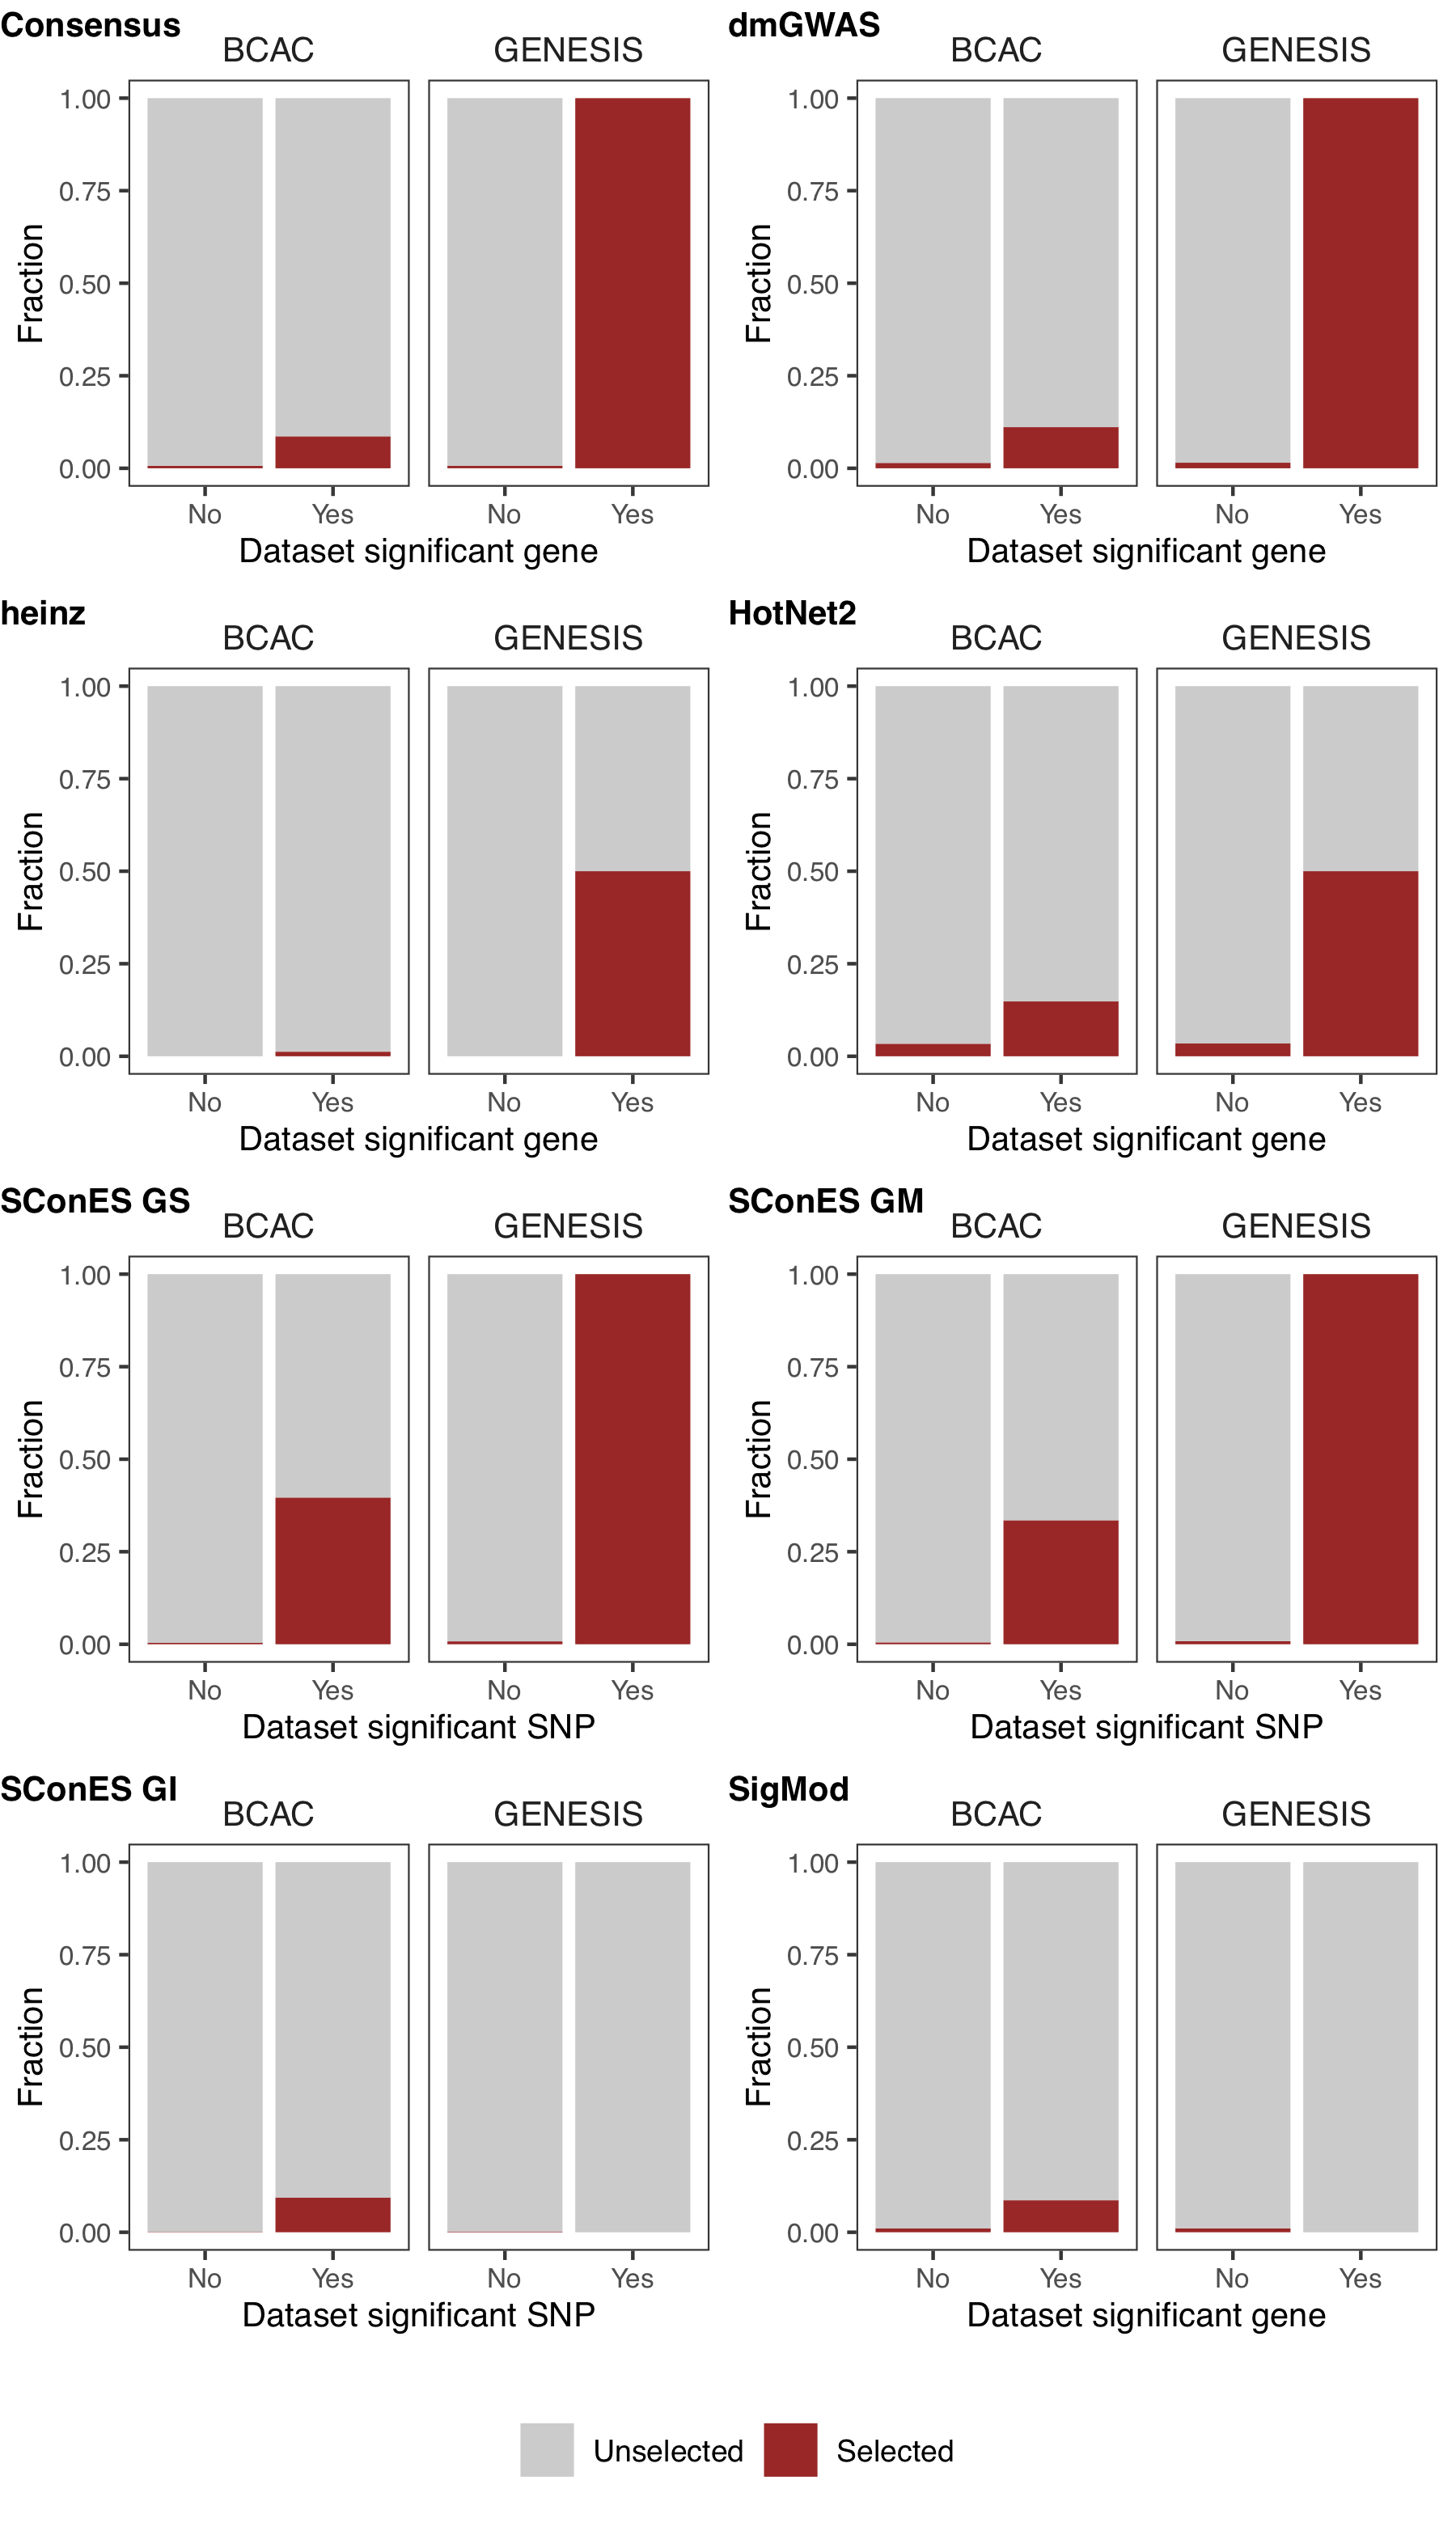
\includegraphics[height=0.8\textheight]{fig/sfigure_4} 

}

\caption{Proportion of the Bonferroni significant biomolecules (in either the GENESIS or the BCAC datasets) selected by each of the methods on the GENESIS data. \textbf{(Consensus, dmGWAS, heinz, HotNet2, and SigMod)} involve significant genes, only among those present in the protein-protein interaction network. \textbf{(SConES GS, GM and GI)} involve significant SNPs. LEAN is not displayed as it did not select any gene. The presented network methods recover a higher proportion of significant genes than of non-significant genes in both datasets, despite their lack of significance in GENESIS.}\label{fig:bcac-comparison}
\end{figure}



\begin{figure}

{\centering 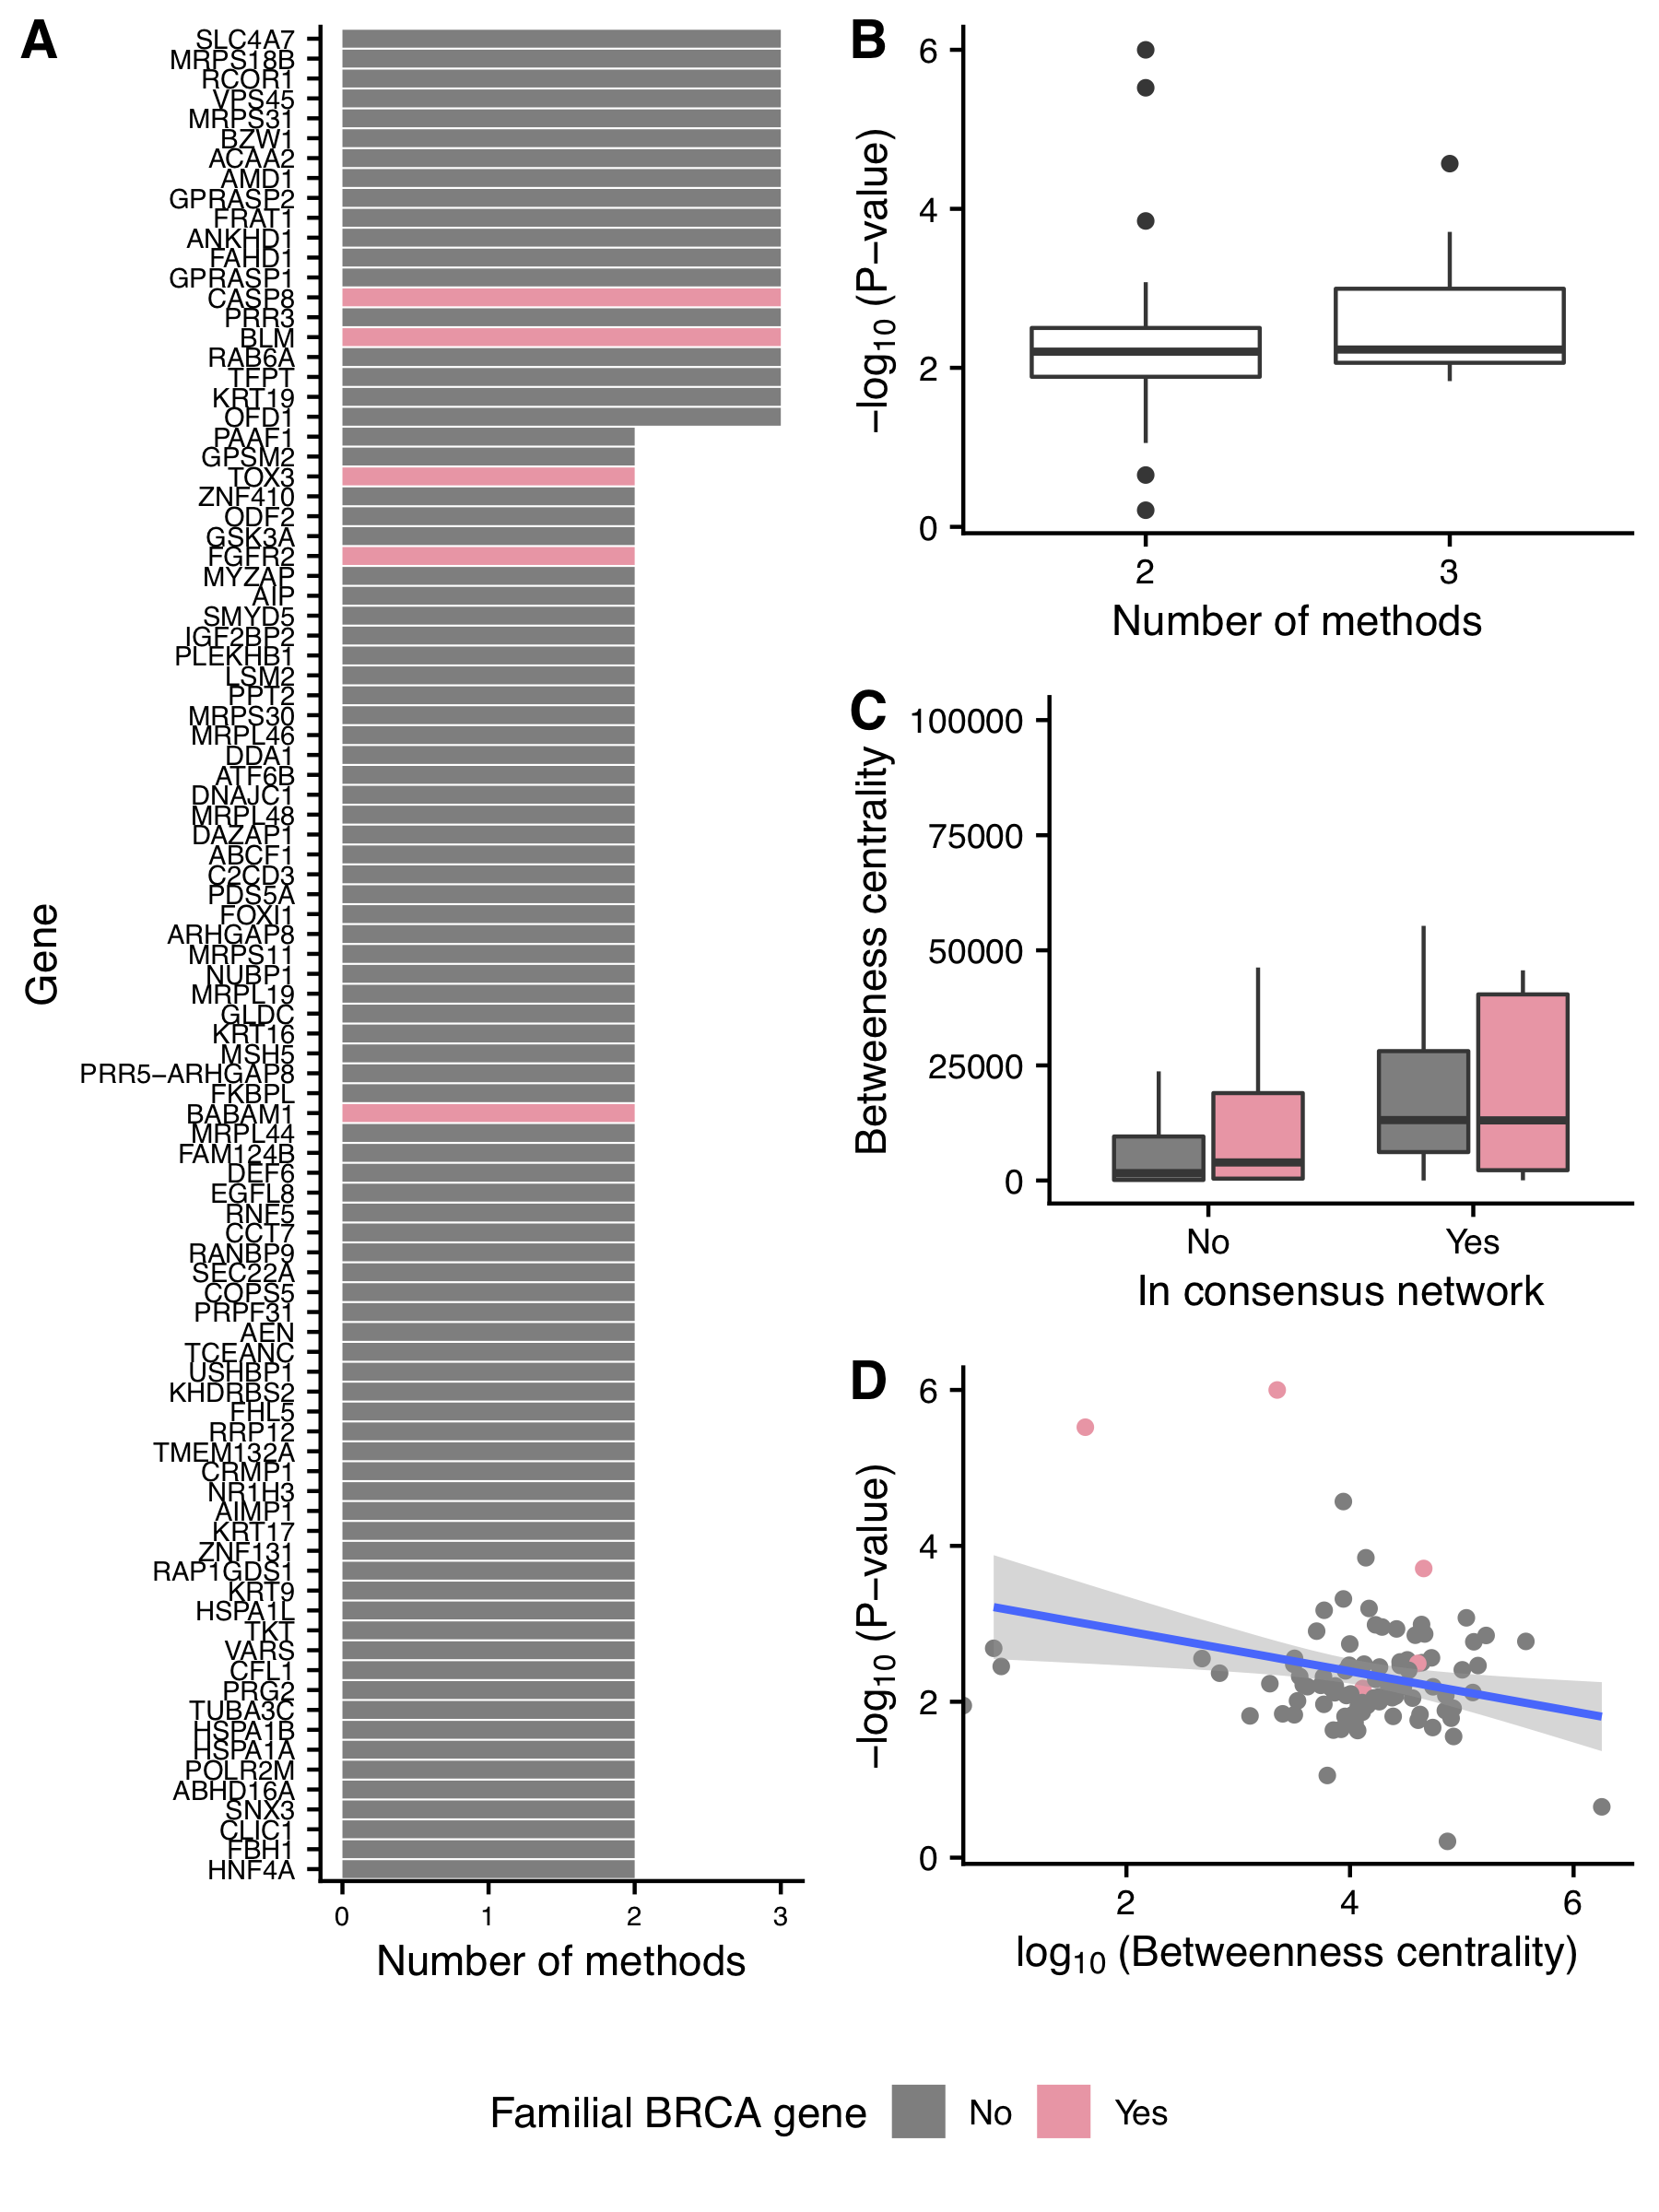
\includegraphics[height=0.75\textheight]{fig/sfigure_8} 

}

\caption{Genes on the consensus network. Breast cancer susceptibility genes are colored in pink; the rest are colored in grey. \textbf{(A)} Number of methods selecting every gene in the subnetwork. \textbf{(B)} VEGAS P-values of association of the genes, with regards to the number of methods that selected them. \textbf{(C)} Comparison of betweenness centrality of the genes in the consensus network and the other genes in the PPIN and not in the consensus network. To improve visualization, we removed outliers. \textbf{(D)} Relationship between the log\textsubscript{10} of the betweenness centrality and the -log\textsubscript{10} of the VEGAS P-value of the genes in the consensus network. The blue line represents a fitted generalized linear model.}\label{fig:consensus-stats}
\end{figure}

As the solutions were quite different from each other it is hard to draw
joint conclusions. The 4-gene solution selected by heinz includes the
breast cancer susceptibility gene \emph{TOX3}, in region 16q12. By dealing
with SNP networks, SConES studies the association of non-coding regions,
as well as SNPs in any gene, coding or not. In fact, SConES GI, which
adds to GM the interactions between genes, retrieves 4 subnetworks in
intergenic regions, and 1 overlapping an RNA gene (\emph{RNU6-420P}). SigMod,
despite being related to SConES, produces a vastly different, large
solution. On top of recovering three breast cancer susceptibility genes,
a keratin-based region of its subnetwork affects the cytoskeleton
(\emph{structural constituent of cytoskeleton}, GO enrichment's adjusted
P-value = 9.10 10\textsuperscript{-4}), a potentially novel susceptibility mechanism for
cancer susceptibility. Interestingly, dmGWAS solution is also related to
cytoskeleton (\emph{tubulin binding}, GO enrichment's adjusted P-value =
0.031). But, additionally, it includes a submodule of proteins related
to \emph{unfolded protein binding} (GO enrichment's adjusted P-value =
0.045), which has been previously related to cancer susceptibility
(Calderwood and Gong \protect\hyperlink{ref-calderwood_heat_2016}{2016}). Lastly, HotNet2 produced 135 subnetworks, 115
of which have less than five genes. The second largest subnetwork (13
nodes), contains the two breast cancer susceptibility genes \emph{CASP8} and
\emph{BLM}.

\hypertarget{results-benchmark}{%
\subsection{heinz retrieves a small, highly informative set of biomarkers in a fast and stable fashion}\label{results-benchmark}}



\begin{figure}

{\centering 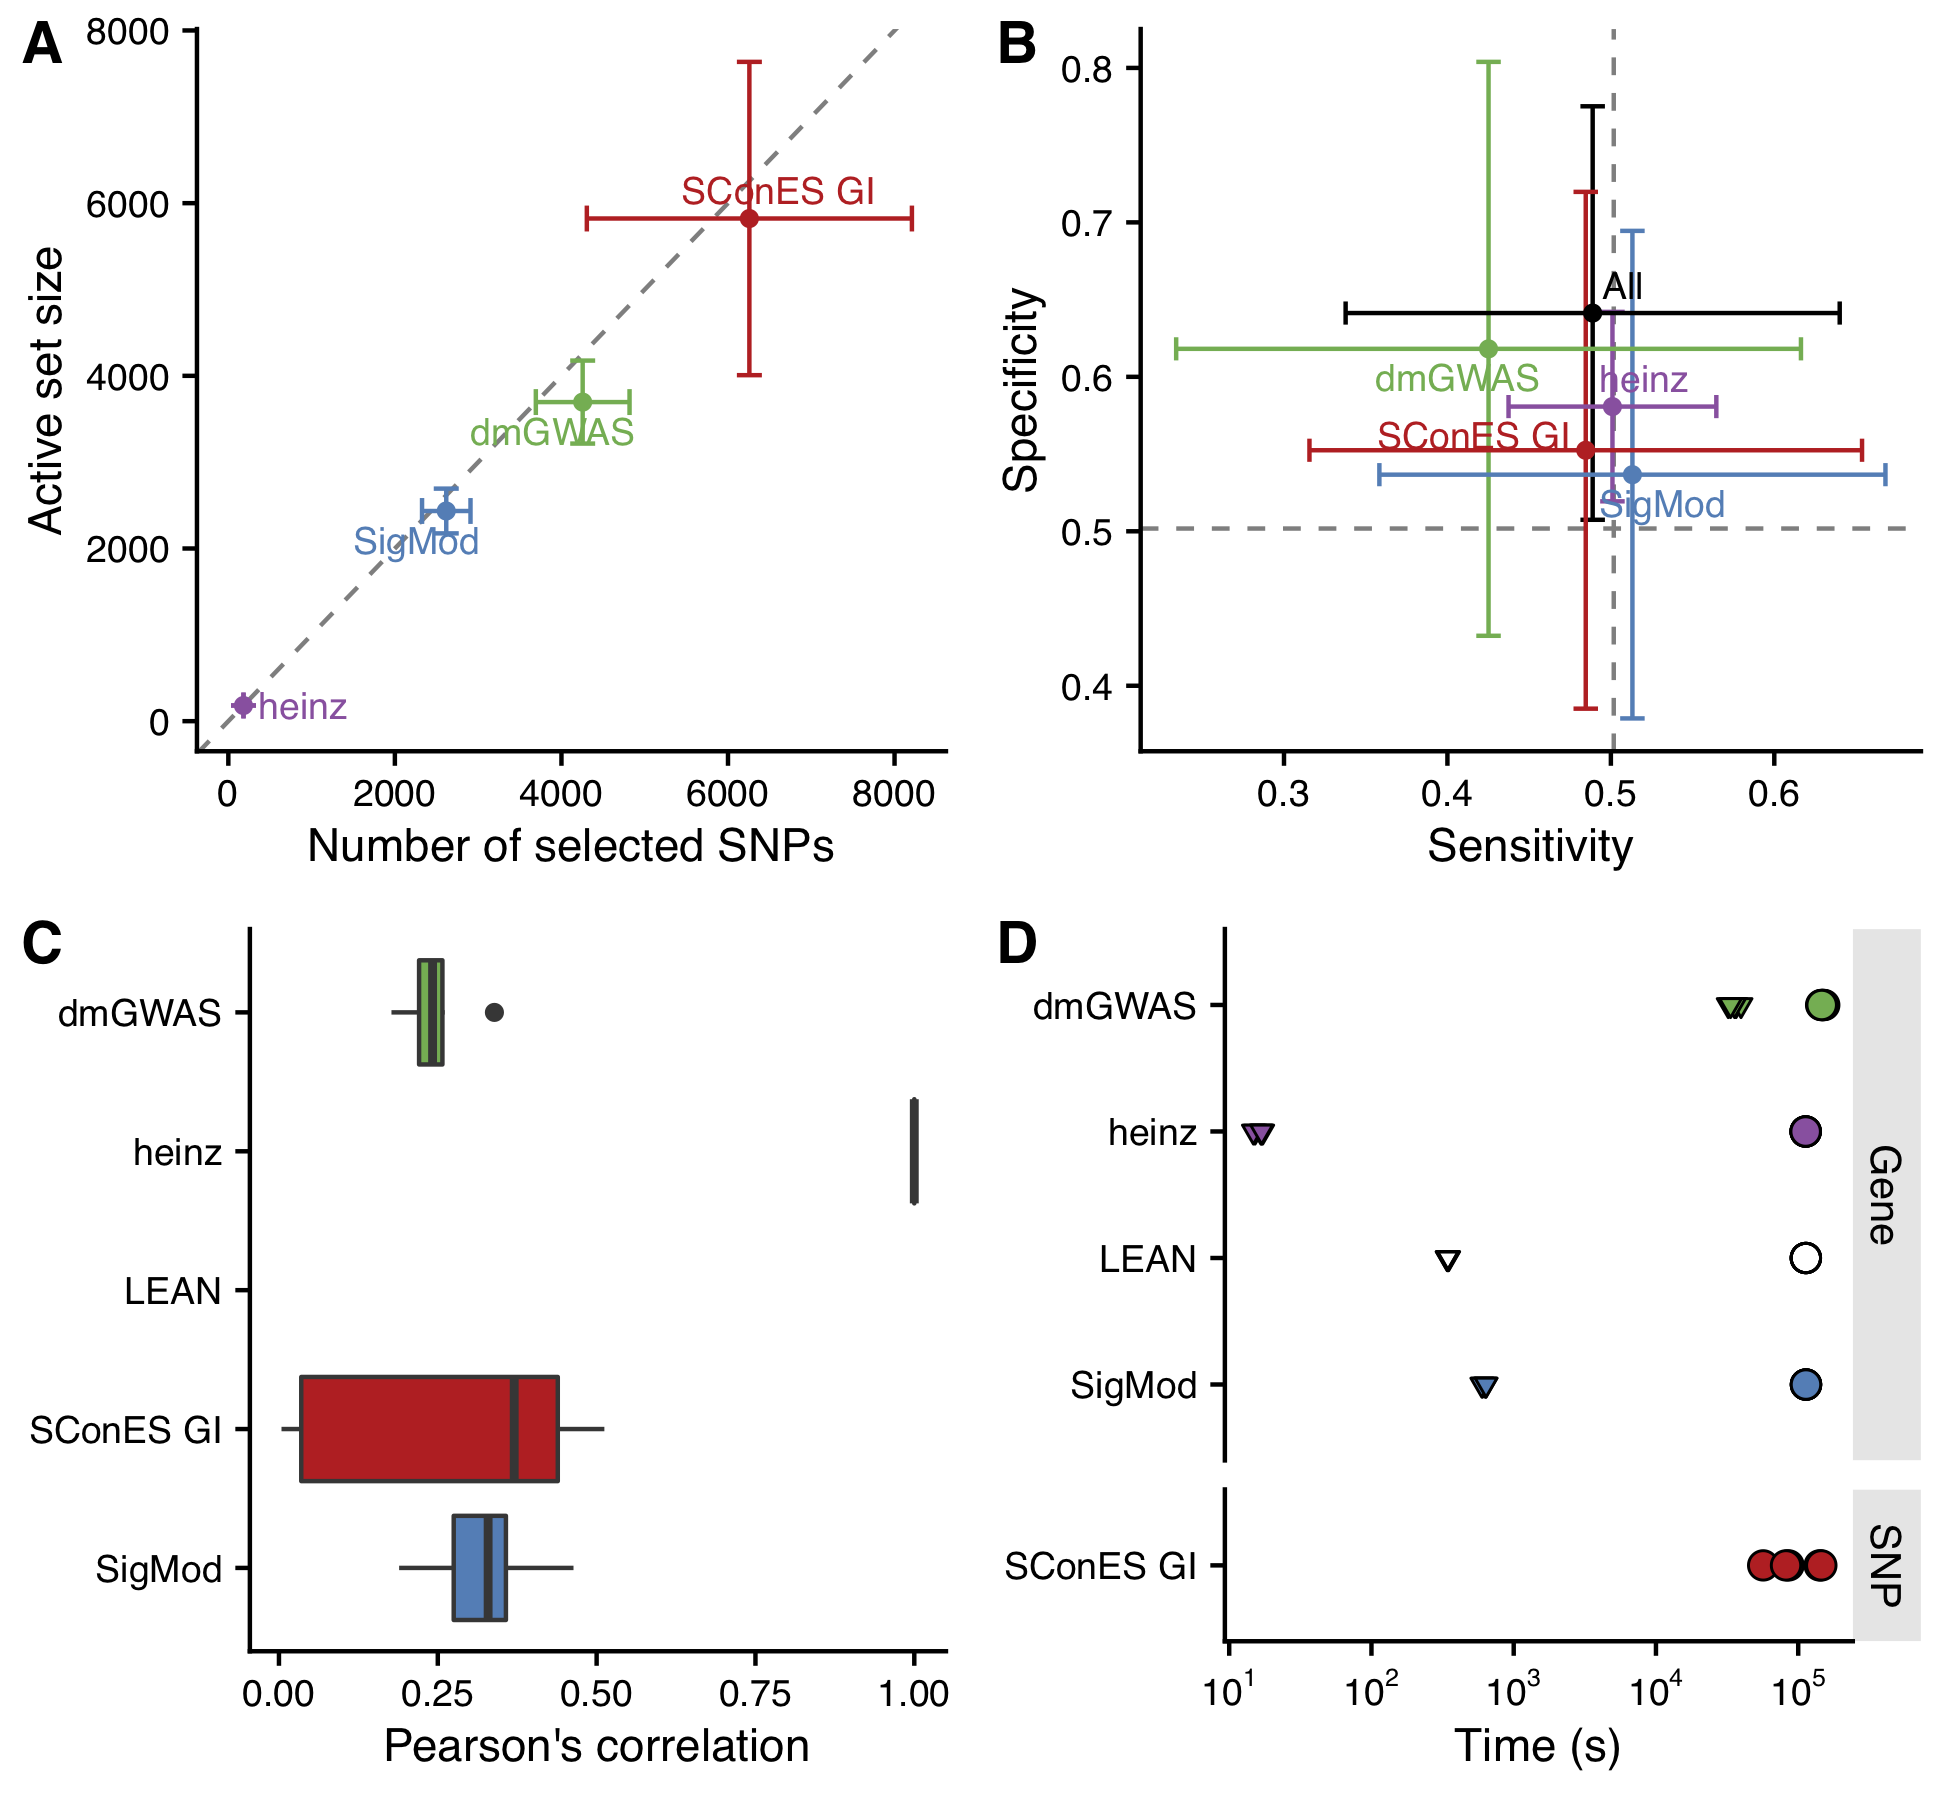
\includegraphics[width=0.8\linewidth]{fig/figure_4} 

}

\caption{Comparison of network-based GWAS methods on GENESIS. Each method was run 5 times of a random subset of the samples, and tested on the remaining samples (Section \ref{methods:comparison}). \textbf{(A)} Number of SNPs selected by each method and number of SNPs on the active set used by the Lasso classifier. Points are the average over the 5 runs; lines represent the standard error of the mean. A grey diagonal line with slope 1 is added for comparison. For reference, the active set of Lasso using all the SNPs included, on average, 154,117.4 SNPs. \textbf{(B)} Sensitivity and specificity on test set of the L1-penalized logistic regression trained on the features selected by each of the methods. In addition, the performance of the classifier trained on all SNPs is displayed. Points are the average over the 5 runs; lines represent the standard error of the mean. \textbf{(C)} Pairwise Pearson\textbackslash's correlations of the solutions used by different methods. A Pearson's correlation of 1 means the two solutions are the same. A Pearson's correlation of 0 means that there is no SNP in common between the two solutions. \textbf{(D)} Runtime of the evaluated methods, by type of network used (gene or SNP). For gene network-based methods, inverted triangles represent the runtime of the algorithm itself, and circles the total time, which includes the algorithm themselves and the additional 119,980 seconds (1 day and 9.33 hours) which took VEGAS2v2 on average to compute the gene scores from SNP summary statistics.}\label{fig:benchmark}
\end{figure}

As the employed methods produced such different results, we compared
their solutions in a 5-fold subsampling setting (Section
\ref{methods:comparison}). Specifically, we measured
four properties (Figure \ref{fig:benchmark}):
size of the solution subnetwork,
sensitivity and specificity of an L1-penalized logistic regression on
the selected SNPs, stability, and computational runtime.

Both solution size and active set of SNPs selected by Lasso varies
greatly between the different methods (Figure \ref{fig:benchmark}A).
heinz has the smallest solutions, with an
average of 182 selected SNPs are selected by
Lasso. The largest solutions come from SConES GI (6256.6 SNPs), and
dmGWAS (4255.0 SNPs). Interestingly, heinz has the highest proportion of
the selected SNPs that go into the active set (99.9\%), although it is
high for all the methods (\textgreater{} 86\%). This suggests methods are selecting
informative SNPs on average.

To determine whether the selected SNPs could be used for patient
classification we computed the sensitivity and the specificity of the
classifier on the testing data (Figure \ref{fig:benchmark}B).
All classifiers' sensitivities were in the
0.42 -- 0.51 range; the specificities, between 0.54 and 0.62. On
average, SigMod had the highest sensitivity (0.51); dmGWAS, the highest
specificity (0.52). Both heinz and SigMod had on average better
sensitivity than the classifier trained on all the SNPs, but none had
superior specificity. However, the differences are negligible, well
within the 95\% confidence interval.

Another desirable quality of an algorithm is stability (Section
\ref{methods:comparison}). Both heinz and LEAN displayed a high
stability in our benchmark, consistently selecting the same genes and no
genes over the 5 subsamples, respectively (Figure \ref{fig:benchmark}C).
Conversely, the other methods displayed similarly low stabilities.

In terms of computational runtime, the fastest method was heinz (Figure
\ref{fig:benchmark}D), which leverages on its ability to find
efficiently the solution in a few seconds. The slowest method was dmGWAS
(1 day and 17 hours on average) followed by SConES GI (1 day and 4.32
hours on average). However, including the time required to compute the gene
scores slows down considerably gene-based methods; on this
benchmark, that step took on average 1 day and 9.33 hours. Considering
that, it took 3 days and 2.4 hours on average for dmGWAS' to produce
results.

\hypertarget{genesis-issues}{%
\subsection{No solution is perfect}\label{genesis-issues}}



\begin{figure}
\centering
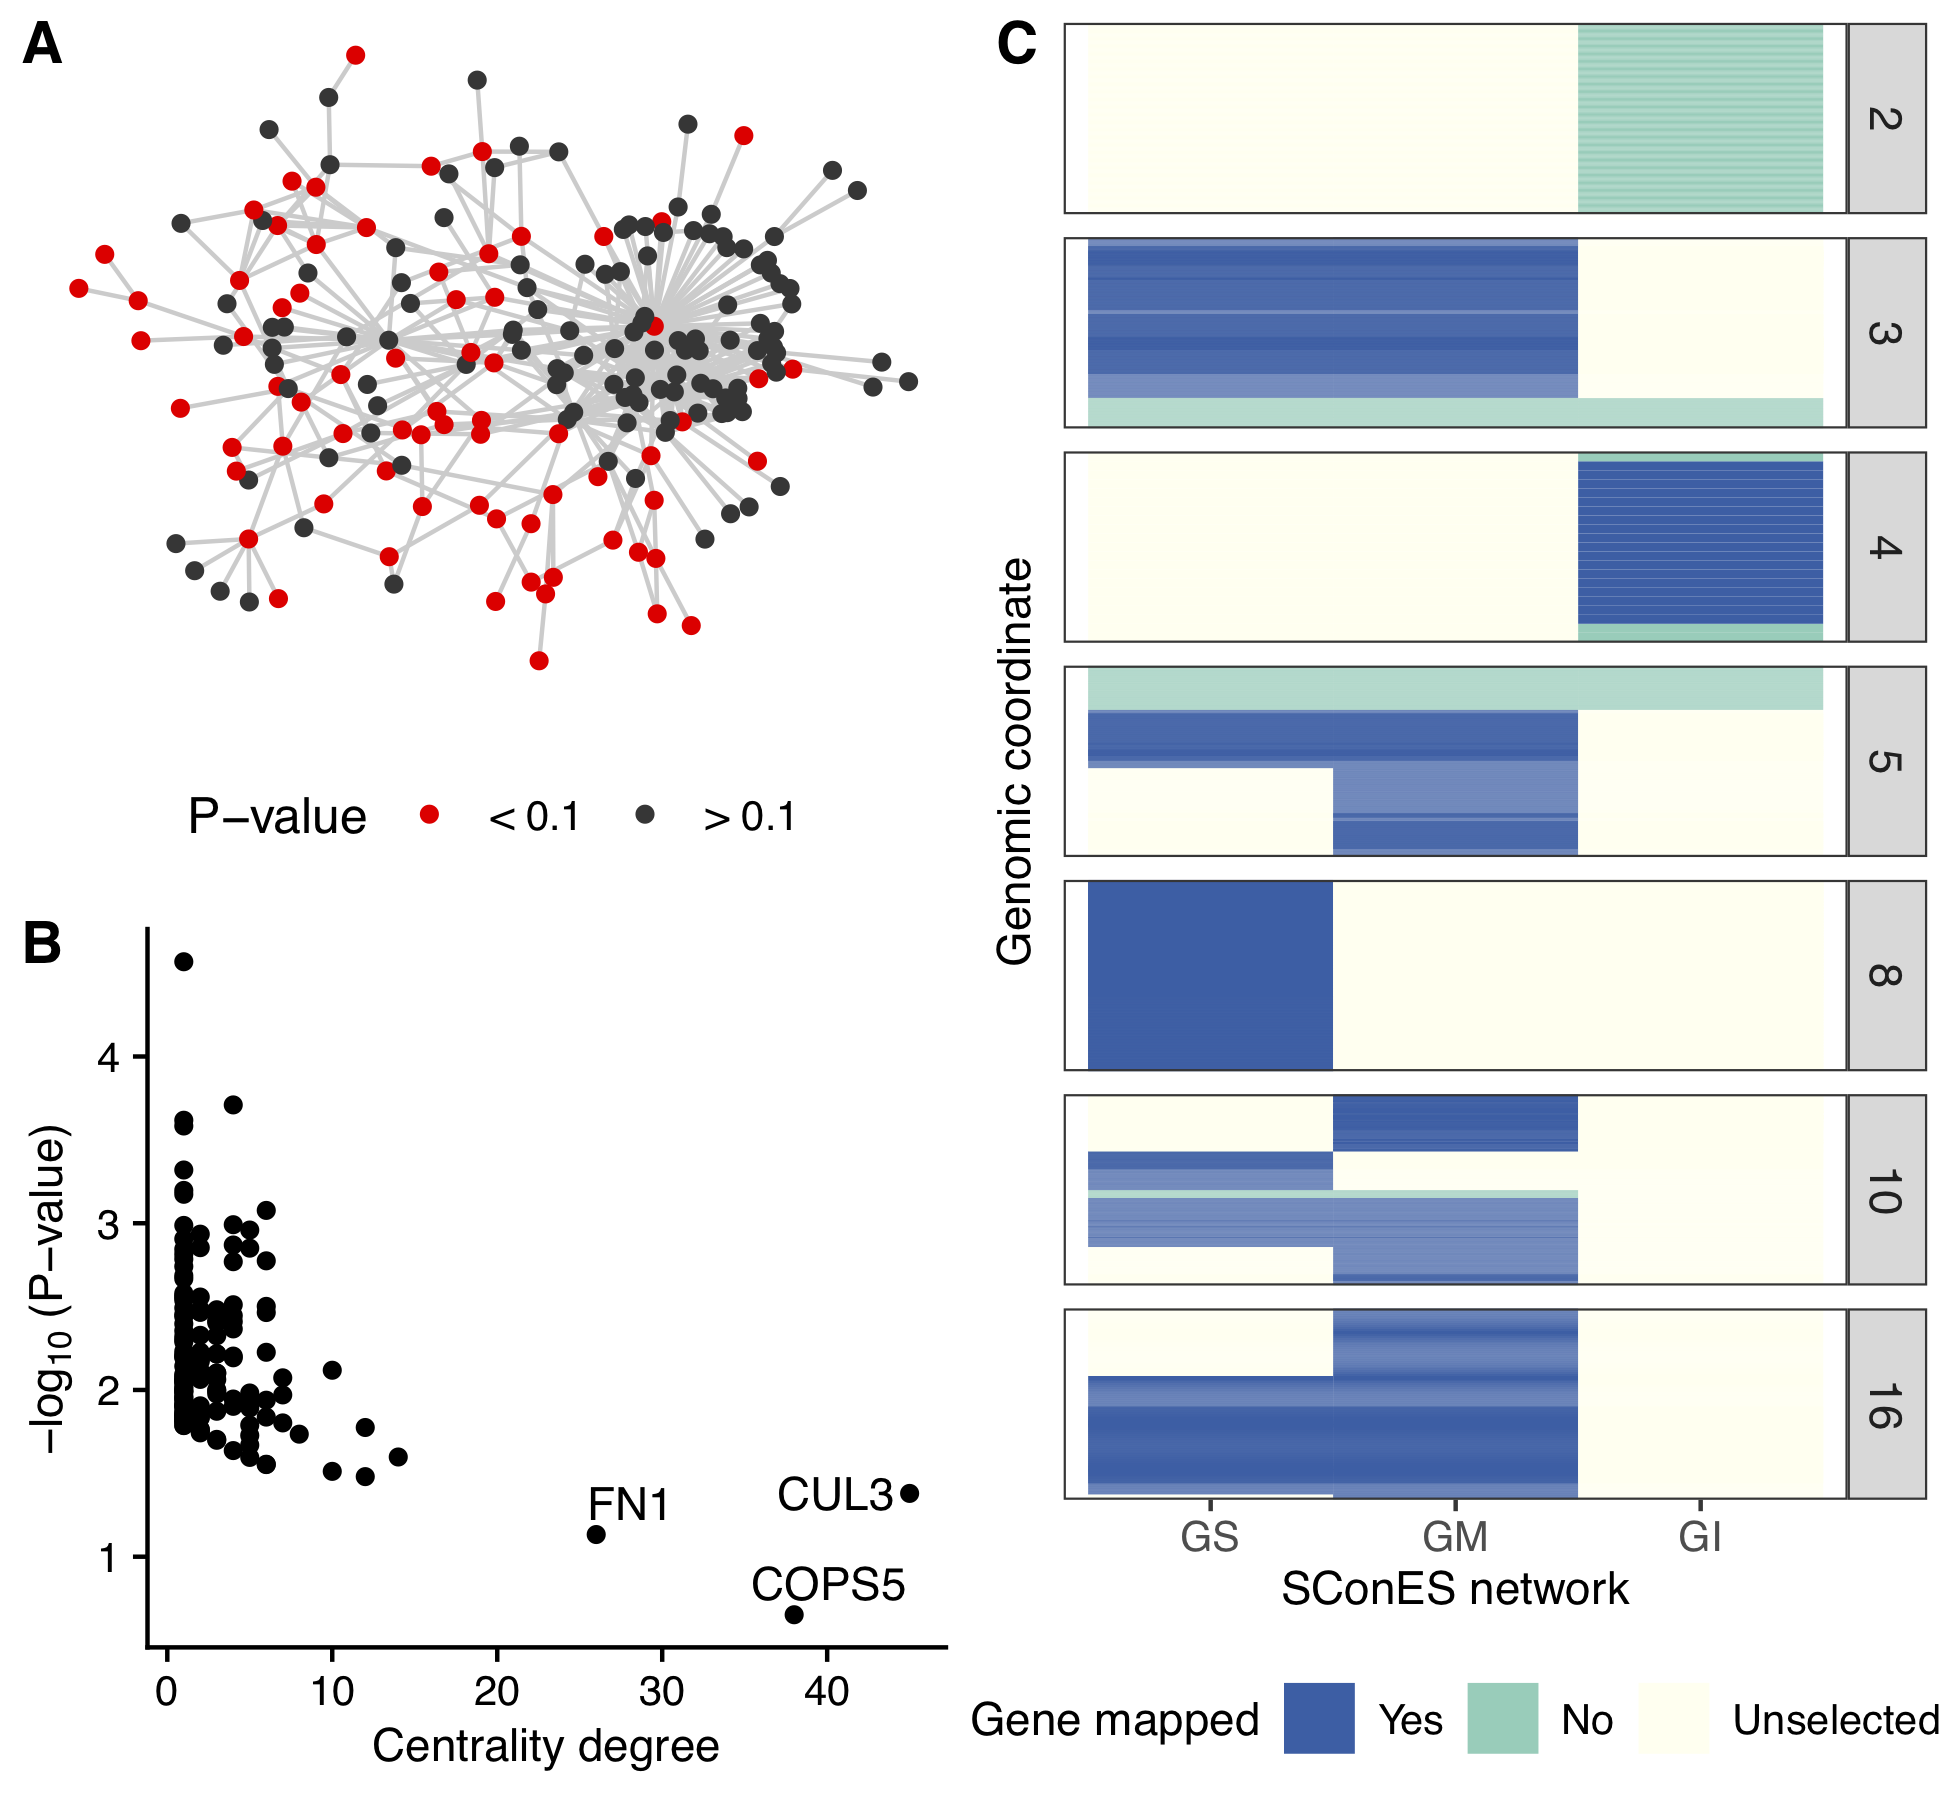
\includegraphics{fig/figure_2.png}
\caption{\label{fig:issues}Drawbacks confronted when using network guided methods. \textbf{(A)} dmGWAS solution subnetwork. Genes with a P-value \textless{} 0.1 are highlighted in red. \textbf{(B)} Centrality degree and -log\textsubscript{10} of the VEGAS P-value for the nodes in SigMod solution subnetwork. \textbf{(C)} Genomic regions where either SConES GS, GM or GI select SNPs.}
\end{figure}

In practice, and despite their similarities and their involvement in
cancer mechanisms, the solutions are remarkably different
(Figure \ref{fig:pearson-methods}A). That is due to the particularities
of the methods which directly or indirectly provide information about
the dataset. For instance, the fact that LEAN did not provide any
biomarkers implies that there is no gene such that both itself and its
environment are on average strongly associated with the disease.



\begin{figure}
\centering
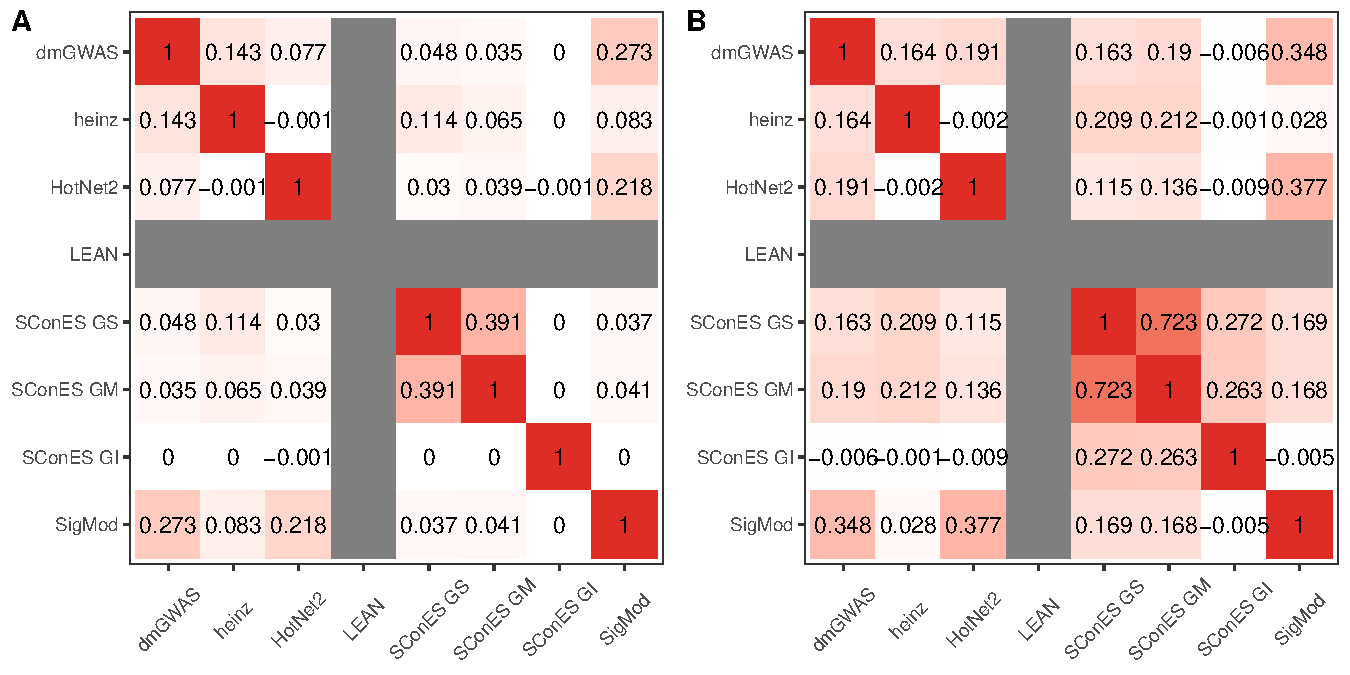
\includegraphics{fig/sfigure_6.pdf}
\caption{\label{fig:pearson-methods}Pearson's correlation between the different solution subnetworks. \textbf{(A)} Correlation between selected SNPs. \textbf{(B)} Correlation between selected genes. In general, the solutions display a very low overlap.}
\end{figure}

In this dataset, heinz's solution is very conservative, providing a
small solution with the lowest median P-value for the subnetwork (Table
\ref{tab:gene-solutions}). Due to this parsimonious and highly
associated solution, it was the best method to select a set of good
biomarkers for classification. (Figure \ref{fig:benchmark}B).
Its conservativeness stems from its
preprocessing step, which models the gene P-values as a mixture model of
a beta and a uniform distribution, controlled by an FDR parameter. Due
to the limited signal at the gene level in this dataset (Figure
\ref{fig:snp-gene-manhattan}B), only 36 of them are retain a
positive score after applying the BUM model (Section
\ref{methods:methods}). Hence, heinz's solution subnetwork
consists only of 4 genes, which does not provide much insight of the
biology of cancer. Importantly, it ignores genes that are strongly
associated to cancer in this dataset like \emph{FGFR2}.

On the other end of the spectrum, we have large solutions provided by
dmGWAS, HotNet2, and SigMod. dmGWAS' subnetwork is the least associated
subnetwork on average. This is due to the greedy framework it uses,
which considers all nodes at distance 2 of the examined, and accepts
weakly associated genes if they are linked to another, strongly
associated one. This is exacerbated when the results of successive
greedy searches are aggregated, leading to a large, tightly connected
cluster of unassociated genes (Figure \ref{fig:issues}A).
SigMod displays the same tendency, as the
most central genes are the least associated to the disease (Figure
\ref{fig:issues}B). This relatively low signal-to-noise ratio
combined with the large solution requires additional analyses to draw
conclusions, such as enrichment analyses. In the same line, HotNet2's
subnetwork is even harder to interpret, being composed of 440 genes
divided into 135 subnetworks. Lastly, SigMod misses some of the most
strongly associated, breast cancer susceptibility genes in the dataset,
like \emph{FGFR2} and \emph{TOX3}.

By virtue of using a SNP subnetwork, SConES analyzes each SNP in their
context. It therefore selects SNPs in genes none of whose interactors
are associated to the disease, as well as SNPs in non-coding regions or
in non-interacting genes. In fact, due to linkage disequilibrium, such
genes are favored by SConES, as selecting SNPs in an LD block which
overlaps with a gene favors selecting the rest of the gene. This might
explain why the GS and GM networks, heavily affected by linkage
disequilibrium, produce similar results (Figure
\ref{fig:pearson-methods}B). On the other hand, SConES penalizes
selecting SNPs and not their neighbors. This makes it conservative
regarding SNPs with many interactions, for instance those mapped to hubs
in the PPIN. For this reason, SConES GI did not select any protein
coding gene, despite selecting similar regions as SConES GS (Figure
\ref{fig:issues}C). In fact SConES GS and SConES GM select
regions related to breast cancer, like 16q12 (\emph{TOX3}, Section
\ref{results:conventional}), 3p24 (\emph{SLC4A7}/\emph{NEK10},
Ahmed et al. (\protect\hyperlink{ref-search_newly_2009}{2009})), 5p12 (\emph{FGF10}, \emph{MRPS30}, Quigley et al. (\protect\hyperlink{ref-quigley_5p12_2014}{2014})), and
10q26 (\emph{FGFR2}, Section \ref{results:conventional}). On top of that only SConES
GS selects region 8q24 (\emph{POU5F1B}, Breyer et al. (\protect\hyperlink{ref-breyer_expressed_2014}{2014})). We hypothesize
that the lack of results on the PPIN network of SConES GI and LEAN due
to the same cause: the absence of joint association of a module.
Although in the case of SConES other hyperparameters could lead to a
more informative solution (e.g.~lower \(\lambda\), Section\ref{methods:methods}),
it is unclear what is the best strategy
to find them. In addition, due to the iCOGS SNP array design, the genome
of GENESIS participants has not been unbiasedly surveyed: some regions
are fine-mapped --- which might distort gene structure in GM and GI
networks --- while others are under studied --- hurting the accuracy
with which the GS network captures the genome structure.

\hypertarget{results:consensus}{%
\subsection{Aggregating solutions provides insights into the biology of cancer}\label{results:consensus}}

To leverage on the strengths of each of the methods and compensate their
respective weaknesses, we built a consensus subnetwork that captures the
mechanisms most shared among the solution subnetworks (Section
\ref{methods:consensus}). The consensus subnetwork (Figure
\ref{fig:consensus-names}) contains 93 genes and is enriched in breast
cancer susceptibility genes (Fisher's exact test P-value = 7.8 10\textsuperscript{-5}).
Due to the limited overlap between methods, only 20 genes were common to
more than two of them (Figure \ref{fig:consensus-stats}A). Encouragingly,
the more methods selected a gene, the higher its association was (Figure
\ref{fig:consensus-stats}B). Globally, a GO enrichment shows the
involvement of two cellular processes: unfolded protein binding, and
structural constituent of cytoskeleton (adjusted P-values of 0.001,
0.001, respectively), which were already observed in different solutions
(Section \ref{results:separate-networks}). Remarkably, many of the
selected genes are related to mitochondrial translation. For instance,
MRPS30 (VEGAS P-value = 0.001), encodes a mitochondrial ribosomal
protein and was also linked to breast cancer susceptibility
(Quigley et al. \protect\hyperlink{ref-quigley_5p12_2014}{2014}). Albeit disconnected from MRPS30, the consensus
network includes a 2-node subnetwork composed of two mitochondrial
ribosomal protein (MRPS31 - VEGAS P-value = 7.67 10\textsuperscript{-3} - and MRPS18B -
VEGAS P-value = 7.92 10\textsuperscript{-3}), which suggests an involvement of
mitochondrial ribosomes in carcinogenesis.



\begin{figure}

{\centering 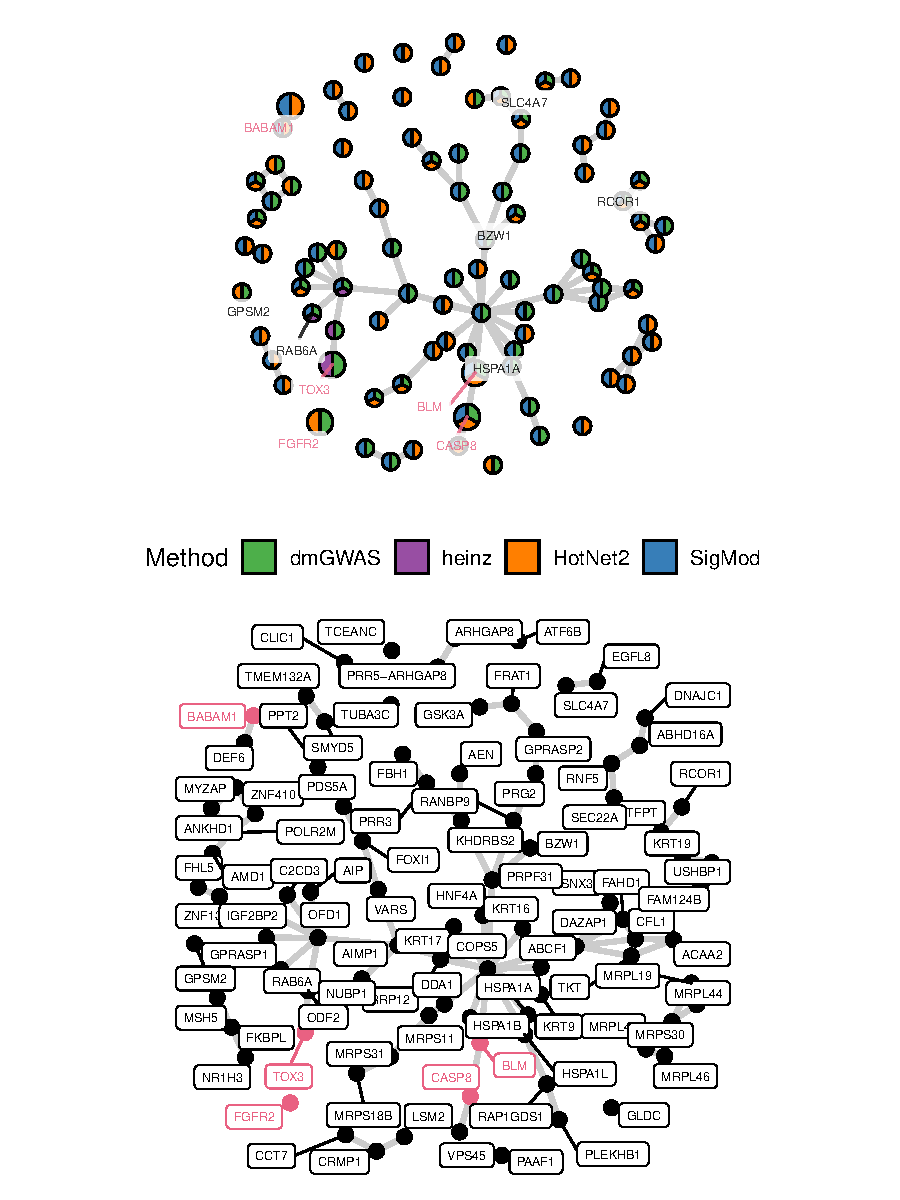
\includegraphics[height=0.8\textheight]{fig/sfigure_7} 

}

\caption{Consensus subnetwork on GENESIS (Section \ref{methods:consensus}). \textbf{(A)} Each node is represented by a pie chart, which shows the methods that selected it. The labeled genes have a VEGAS2v2 P-value \textless{} 0.001 and/or are known breast cancer susceptibility genes (colored in pink). \textbf{(B)} The name of every gene is indicated.}\label{fig:consensus-names}
\end{figure}

We also examined the topological properties of the nodes. The genes in
the consensus network have higher betweenness centrality than the rest
of the genes (Wilcoxon rank-sum test P-value = 4.29 10\textsuperscript{-18}).
Interestingly, within genes in the consensus network, cancer genes are
as central as non-cancer genes (Wilcoxon rank-sum test P-value = 0.57).
Centrality, however, is weakly anti-correlated with association to the
disease (Pearson correlation coefficient = -0.26, Figure
\ref{fig:consensus-stats}D), which suggests that some highly
central genes were selected because they were on the shortest path
between two highly associated genes. In view of this, we hypothesize
that highly central genes might contribute to the heritability through
consistent alterations of their neighborhood, consistent with the
omnigenic model of disease (Boyle, Li, and Pritchard \protect\hyperlink{ref-boyle_expanded_2017}{2017}). For instance, the
most central node in the consensus network is \emph{COPS5}
(Figure \ref{fig:consensus-names}), a gene related to multiple hallmarks
of cancer and which is overexpressed in multiple tumors, including
breast and ovarian cancer (G. Liu et al. \protect\hyperlink{ref-liu_jab1_cops5_2018}{2018}). Despite its lack of
association in GENESIS (VEGAS P-value = 0.22), its neighbors in the
consensus subnetwork have consistently low P-values (median VEGAS
P-value = 0.006).

The consensus subnetwork is not completely connected: out of the 93
genes, the largest connected subnetwork includes only 49. A GO
enrichment analysis showed that this component is related to three major
cellular processes: unfolded protein binding, structural constituent of
cytoskeleton, and poly(U) RNA binding (adjusted P-values of 0.01, 0.04,
and 0.04, respectively). We found support in the literature of the
involvement of each of these functions in the development of cancer, as
discussed next. The consensus network also contains a protein directly
involved in caspase-mediated apoptosis, \emph{CASP8} (VEGAS P-value = 1.95
10\textsuperscript{-4}). This is related to the enriched activity, \emph{unfolded protein
binding}, which inhibits caspase-dependent apoptosis, raising the
chances of developing cancer (Calderwood and Gong \protect\hyperlink{ref-calderwood_heat_2016}{2016}). It involves three
Hsp70 chaperones of the consensus subnetwork: HSPA1A, HSPA1B, and
HSPA1L. They genes encoding these proteins are all near each other at
6p21. In fact, out of the 22 SNPs that map to any of these three genes,
9 map to all of them, and 4 to two, making hard to disentangle their
association. \emph{HSPA1A} was the most strongly associated one (VEGAS P-value
= 8.37 10\textsuperscript{-4}). Remarkably, 14 of the 93 genes are in subnetworks of
size 1 (isolated) or 2, as they do not have a consistently altered
neighborhood. One of them is the well-known breast cancer susceptibility
gene \emph{FGFR2} (Section \ref{results:conventional}
). Another one is the also well-known
\emph{SLC4A7} gene (VEGAS P-value = 2.70 10\textsuperscript{5}), which encodes a sodium
bicarbonate cotransporter. The genomic region containing both \emph{SLC4A7}
and nearby gene \emph{NEK10} (VEGAS P-value = 1.56 10\textsuperscript{-5}) have been
consistently associated with breast cancer susceptibility
(Ahmed et al. \protect\hyperlink{ref-search_newly_2009}{2009}). \emph{NEK10} is a gene that might be involved in
cell-cycle control, but it is absent from the PPIN and hence it could
not be studied by gene methods. Despite that, the fact that both dmGWAS,
HotNet2 and SigMod link \emph{SLC4A7} in their different subnetwork supports
the notion that this gene is the responsible for breast cancer
susceptibility.

\hypertarget{genewa-discussion}{%
\section{Discussion}\label{genewa-discussion}}

In this chapter we evaluate the viability of systems biology approaches
to GWAS, and examine a GWAS dataset on familial breast cancer focused on
\emph{BRCA1/2} negative French women. Systems biology addresses two of the
largest GWAS issues: interpretability and an overly conservative
statistical framework that hinders discovery. This is achieved by
considering the biological context of each of the genes and SNPs. Based
on divergent considerations of what the desired set of biomarkers is,
several methods for network-guided biomarker discovery have been
proposed. We reviewed the performance of six of them on GWAS. Despite
their differences, most of them produced a relevant subset of
biomarkers, recovering known familial breast cancer genes. We also
discuss the limitations of such analyses, related to the lack of known
interactions around some genes. A crucial step for the gene based
methods is the computation of the gene score. In this chapter we used
VEGAS2v2 (Mishra and Macgregor \protect\hyperlink{ref-mishra_vegas2:_2015}{2015}) due to the flexibility it offers to use
user-specified gene annotations. However, it presents known problems
(selection of an appropriate percentage of top SNPs, long runtimes and
P-value precision limited to the number of permutations
(Nakka, Raphael, and Ramachandran \protect\hyperlink{ref-nakka_gene_2016}{2016})), other algorithms might have more statistical power.

The network methods we studied differ in what the optimal solution
subnetwork looks like. On the one hand, SConES and heinz prefer small
highly associated solutions. On the other hand, SigMod and dmGWAS
gravitate towards larger, less associated solutions which provide a wide
overview of the biological context. While the former provide a reduced
set of biomarkers, the latter deepen our understanding of the disease
and provide biological hypotheses. Yet, they are not exempt of limitations.
dmGWAS and SigMod's solution's size require further analyses, which risk
oversimplifying their richness. Also, incautious practitioners might be
misled by some genes, which are very central in the solution
subnetworks, while being weakly associated. Nonetheless, they are pushed
into the solution by their privileged topological properties. On the
other end, conservative solutions, like SConES GI and heinz might not
shed much light on the etiology of the disease.

To overcome the problems posed by the individual methods while
exploiting their strengths, we propose combining them into a consensus
subnetwork. We use a straightforward aggregation to generate it,
including any node that was recovered by at least two methods. The
resulting network is a synthesis of the altered mechanism: it is smaller
than the largest solutions (SigMod and dmGWAS), which makes it more
manageable, and includes the majority of the strongly associated smaller
solutions (SConES and heinz). The consensus subnetwork captures
mechanisms and genes known to be related to cancer, recovering known
breast cancer susceptibility genes as well as genome regions associated
to breast cancer susceptibility. However, thanks to its smaller size and
its network structure, it provides compelling hypotheses of
non-canonical mechanisms involved in carcinogenesis, like mitochondrial
translation and chaperone activity.

The strength of network-based analyses comes from leveraging prior
knowledge to boost discovery. In consequence, they show their
shortcomings in front of understudied genes, especially those not in the
network. Out of the 32,767 genes that we can map the genotyped SNPs to,
60.7\% (19,887) are not in the protein-protein interaction network. The
majority of those (14,660) are non-coding genes, mainly lncRNA, miRNA,
and snRNA (Figure \ref{fig:biotypes-excluded}). The importance of these genes,
like \emph{CASC16}, is highlighted in Section \ref{results:conventional}.
Among the excluded protein-coding
genes we find genes like \emph{NEK10} (P-value 1.6 10\textsuperscript{-5}) or \emph{POU5F1B}, both
linked to breast cancer susceptibility (Ahmed et al. \protect\hyperlink{ref-search_newly_2009}{2009}). However, on
average protein-coding genes absent from the PPIN are less associated
with this phenotype (Wilcoxon rank-sum P-value = 2.79 10\textsuperscript{-8}, median
P-values of 0.43 and 0.47). As we are using interactions from
high-throughput experiments, such difference cannot be due to well-known
genes having more known interactions. As disease genes tend to be more
central (Piñero et al. \protect\hyperlink{ref-pinero_uncovering_2016}{2016}), we hypothesize that it is due to
interactions between central genes being more likely. It is worth noting
that network approaches that do not use PPIs, like SConES GS and GM, did
recover SNPs in \emph{NEK10} and \emph{CASC16}. Lastly, all the methods rely
heavily on how SNPs are mapped to genes. In Section
\ref{results:conventional} we highlight ambiguities that appear
when genes overlap or are in linkage disequilibrium.

\begin{figure}
\centering
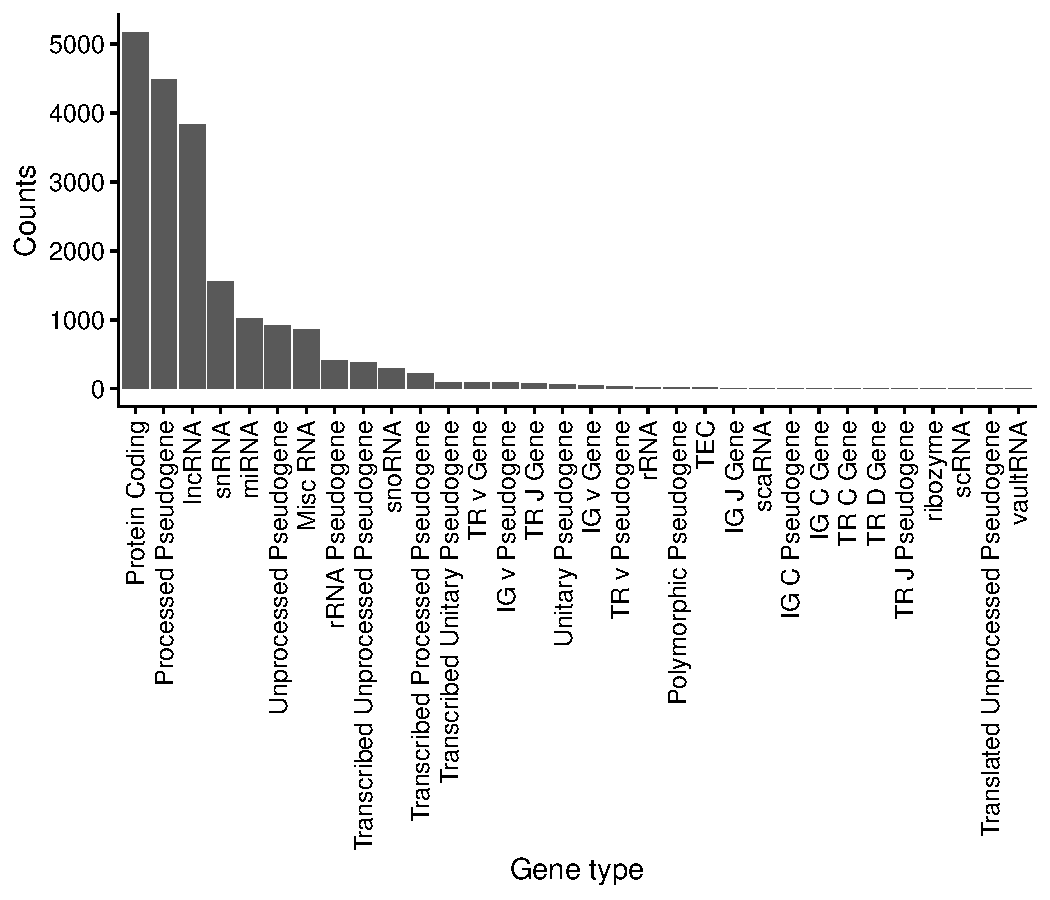
\includegraphics{fig/sfigure_9.pdf}
\caption{\label{fig:biotypes-excluded}Biotypes of genes from the annotation that are not present in the HINT protein-protein interaction network.}
\end{figure}

As not all databases compile the same interactions, the choice of the
PPIN determines the final output. In this work we used exclusively
interactions from HINT from high-throughput experiments. This responds
to concerns of some authors about biases introduced by adding
interactions coming from targeted studies in the literature
(Cai, Borenstein, and Petrov \protect\hyperlink{ref-cai_broker_2010}{2010}; Das and Yu \protect\hyperlink{ref-das_hint_2012}{2012}) where a ``rich getting richer''
phenomenon is observed: popular genes have a higher proportion of their
interactions described. On the other hand, Huang et al. (\protect\hyperlink{ref-huang_systematic_2018}{2018}) found that the best
predictor of the performance of a network for disease gene discovery is
the size of the network. This also supports
using the largest amount of interactions. To clarify their impact on
this study, we compared the impact of using only physical interactions
from high-throughput experiment versus interactions from both
high-throughput and the literature (Section \ref{methods:gene-network}). We
conclude that for most of the methods a larger network did not greatly impact
the size or the stability of the solution, the classification accuracy, or the
runtime (Figure \ref{fig:lc-ht-comparison}).



\begin{figure}
\centering
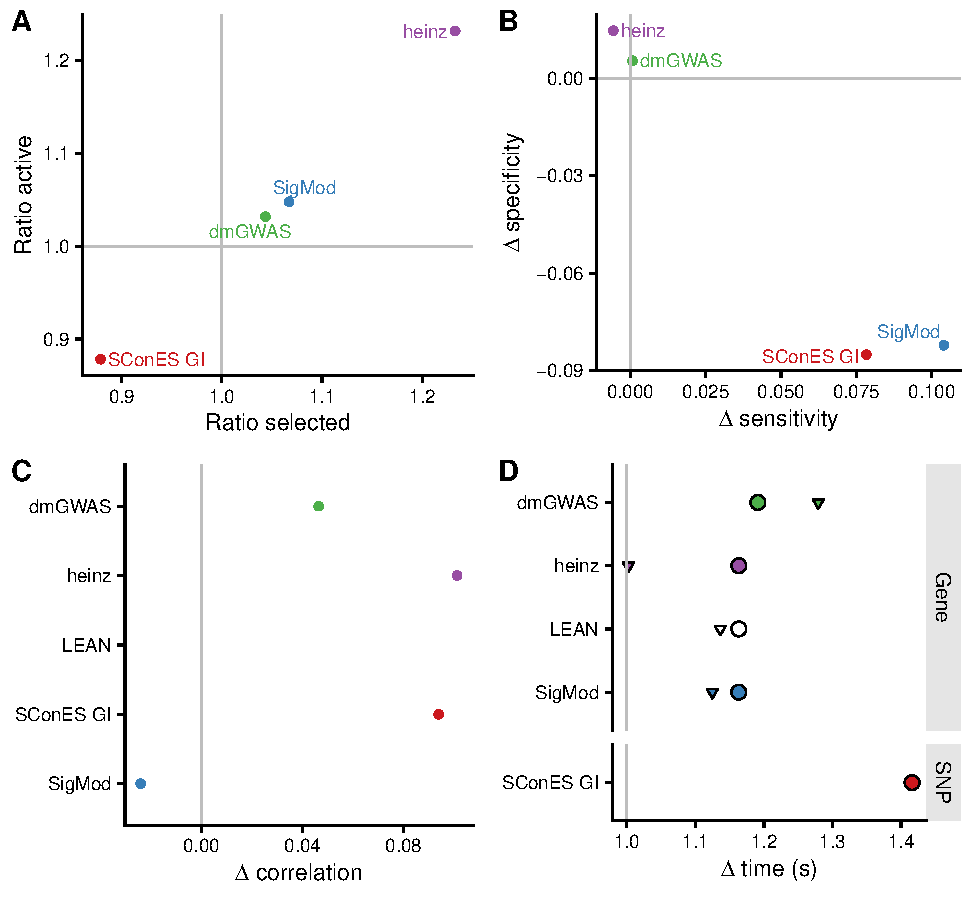
\includegraphics{fig/sfigure_10.pdf}
\caption{\label{fig:lc-ht-comparison}Comparison of benchmark on high-throughput interactions to benchmark on both high-throughput and literature curated interactions. Grey lines represent no change between the benchmarks (1 for ratios, 0 for differences). \textbf{(A)} Ratios of the selected features between both benchmarks and of the active set. \textbf{(B)} Shifts in sensitivity and specificity. \textbf{(C)} Shift in Pearson's correlation between benchmarks. \textbf{(D)} Ratio between the runtimes of the benchmarks. For gene network-based methods, inverted triangles represent the ratio of runtimes of the algorithms themselves, and circles the total time, which includes the algorithm themselves and the additional 119,980 seconds (1 day and 9.33 hours) which took VEGAS2v2 on average to compute the gene scores from SNP summary statistics. In general, adding additional interactions slightly improves the stability of the solution, but increases the solution size, has mixed effects on the sensitivity and specificity, and impacts negatively the required runtime of the algorithms.}
\end{figure}

In order to produce the consensus network, we had to face the different
interfaces, preprocessing steps, and unexpected behaviors of the various
methods. To facilitate that other authors apply them to new datasets and
aggregate their solutions, we built six nextflow pipelines
(Di Tommaso et al. \protect\hyperlink{ref-di_tommaso_nextflow_2017}{2017}) with a consistent interface and, whenever
possible, parallelized computation. They are available on GitHub:
\url{https://github.com/hclimente/gwas-tools}.

\hypertarget{martini}{%
\chapter{\texorpdfstring{The \emph{martini} R package}{The martini R package}}\label{martini}}

Parts of this work were presented in ISMB/ECCB 2017 in the poster \emph{Héctor Climente-González and Chloé-Agathe Azencott}, R package for network-guided Genome-Wide Association Studies.

\begin{chapabstract}{Abstract:}
In this chapter I introduce martini and \verb|scones.nf|. martini is an implementation of SConES in R with three improvements over previous ones. First, it includes measures of association for binary traits ($\chi^2$ and logistic regression). Second, it accepts user-specified covariates, included as additional terms in the logistic regression. Third, it includes four ways of scoring the cross-validation folds: consistency (as other implementations), and three penalized log-likelihood measures (BIC, AIC, and AICc). martini is available in Bioconductor 3.7. \verb|scones.nf| is a computational package that further facilitates the usage of martini. It does so by accepting common file formats for GWAS and networks, and by performing a two-staged cross-validation that achieves better hyperparameters. \verb|scones.nf| is available on \url{https://github.com/hclimente/gwas-tools}.
\end{chapabstract}
\vskip 0.2in
\begin{chapabstract}{Résumé :}
Dans ce chapitre, je pr\'esente martini et \verb|scones.nf|. martini est 
une impl\'ementation en R de SConES, qui pr\'esente trois am\'eliorations sur 
les impl\'ementations pr\'ec\'edentes. Tout d'abord, martini inclut des 
mesures d'association pour des traits binaires ($\chi^2$ et r\'egression 
logistique). Deuxi\`emement, martini permet de sp\'ecifier des covariables, 
incorpor\'ees comme des termes suppl\'ementaires dans la r\'egression 
logistique. Troisi\`emement, martini inclut quatre façons de mesurer la 
performance en validation crois\'ee : la consistance (comme pr\'ec\'edemment), 
et trois mesures de log-vraisemblance p\'enalis\'ee (BIC, AIC and AICc). 
martini est disponible dans Bioconductor 3.7. \verb|scones.nf| est un paquet 
logiciel qui facilite encore plus l'utilisation de martini, en acceptant 
des formats de fichiers usuels pour les donn\'ees GWAS ainsi que les 
r\'eseaux, et gr\^ace \`a une validation crois\'ee en deux \'etapes qui permet 
d'obtenir de meilleurs hyperparam\`etres. \verb|scones.nf| est disponible 
sur \url{https://github.com/hclimente/gwas-tools}.
\end{chapabstract}

\hypertarget{introduction-1}{%
\section{Introduction}\label{introduction-1}}

In Chapter \ref{genesis} I presented six high-score subnetwork search methods, and their application to GWAS. In this chapter I focus on my work on one of them, SConES (Azencott et al. \protect\hyperlink{ref-azencott_efficient_2013}{2013}), which was presented with the other methods in Section \ref{methods:methods}. As a reminder, SConES finds a small set of highly interconnected SNPs associated to the disease by solving the following problem:

\begin{equation}
\underset{S \subseteq G}{\arg \max } \underbrace{\sum_{v \in V_S} s_v}_{\text { association }}-\underbrace{\lambda \sum_{v \in V_S} \sum_{u \not\in V_S} W_{vu} }_{\text { connectivity }}-\underbrace{\eta \lvert V_S \rvert }_{\text { sparsity }},
\end{equation}

where \(\lambda\) and \(\eta\) are hyperparameters, \(s_v\) is the association score of node \(v\), and \(W\) is the Laplacian matrix of the network. The mathematical notation is described in Section \ref{methods:notation}. SConES works on SNP networks in which the SNPs are linked to each other if there is evidence of shared function, for instance, if they are mapped to the same gene (Section \ref{intro-interpretability}).

With the goal of applying SConES to the GENESIS dataset (Section \ref{genesis-dataset}), I developed a user-friendly version that solved some of SConES' initial shortcomings (detailed in Section \ref{martini-improvements}). The result was an R package, \emph{martini} (Climente-González and Azencott \protect\hyperlink{ref-martini}{2019}), which was published in Bioconductor 3.7 (Huber et al. \protect\hyperlink{ref-bioconductor}{2015}), a peer-reviewed R repository. \emph{martini} was the R version (``user friendly'') of \emph{gin} (GWAS Incorporating Networks), which is my \verb!C++! re-implementation of SConES based, in turn, on EasyGWAS (Grimm et al. \protect\hyperlink{ref-grimm_easygwas_2017}{2017}). Hence, \emph{martini} combines the accessibility of R and of the Bioconductor environment with the computational efficiency of \verb!C++!.

\hypertarget{martini-improvements}{%
\section{Improvements over SConES}\label{martini-improvements}}

\hypertarget{covariates-and-additional-measures-of-association}{%
\subsection{Covariates and additional measures of association}\label{covariates-and-additional-measures-of-association}}

SConES scored the relevance of each SNP to the phenotype using the linear SKAT test of association (Wu et al. \protect\hyperlink{ref-wu_rare-variant_2011}{2011}; Ionita-Laza et al. \protect\hyperlink{ref-ionita-laza_sequence_2013}{2013}). Yet, no version of SConES implemented a way to measure association with a binary phenotype, like logistic regression-based SKAT. Hence, we decided to implement two additional measures of association in \emph{martini}, \(\chi^2\) and logistic regression, to apply SConES on case-control studies. Additionally, the latter allowed \emph{martini} to handle covariates and hence correct for population structure (Section \ref{pop-structure}).

\hypertarget{hyperparameter-optimization}{%
\subsection{Hyperparameter optimization}\label{hyperparameter-optimization}}

By examining the results of other implementations of SConES on simulated examples, we observed that it produced suboptimal solutions. Those (unshown) results were either trivial ones (all SNPs or no SNP retrieved), or cases where SNPs strongly associated with a phenotype were not selected. To address those issues, I experimented with altering how SConES chooses its hyperparameters (\(\lambda\) and \(\eta\)), in the hope that other values would produce better solutions.

SConES chooses the best \(\lambda\) and \(\eta\) based on consistency across 10 cross-validation folds. In other words, for each specific combination of \(\lambda\) and \(\eta\) to evaluate, the data is divided into 10 equal parts, or folds, each containing 90\% of the samples. In each fold, a selection vector \(v\) is produced with the respective hyperparameters. The length of \(v\) is equal to the number of SNPs \(N\), and each element is set to 0, if the corresponding SNP is not selected, and to 1, if it is. The consistency \(C\) between the selection vectors \(v_i\) and \(v_j\) of two folds for the same \(\lambda\) and \(\eta\) can be calculated as

\[ C = N\|v_i \cdot v_j \|_0 - \|v_i\| _0\|v_j\|_0 .\]

Then a normalized consistency \(C'\) is computed by dividing \(C\) by the maximum possible consistency \(C^*\):

\[C^* = N \min(\|v_i\| _0, \|v_j\|_0) - \|v_i\| _0\|v_j\|_0. \]

Each combination of \(\lambda\) and \(\eta\) is scored using the mean of all such pairwise normalized consistencies. The hyperparameters that produce the most consistent result are used on the whole dataset to produce the algorithm's output. Consistency was the metric of choice in the original SConES to favor stability in the solution (Azencott et al. \protect\hyperlink{ref-azencott_efficient_2013}{2013}).

We explored alternatives to consistency as selection criterion. Measures based on the accuracy of a linear classifier trained on the selected SNPs had been tested before, but exhibited proneness to overfitting. Hence we turned to penalized log-likelihood measures (Dziak, Li, and Collins \protect\hyperlink{ref-Dziak2005}{2005}), developed in the field of information theory. These scoring functions had the potential to overcome the overfitting of a linear classifier by adding a regularization term to improve generalization. They take the form

\[L(X,y,\hat{\theta})-c(\hat{\theta}),\]

where \(L(X,y,\hat{\theta})\) is the log-likelihood of the model, which depends on the feature matrix \(X\), the outcome vector \(y\), and the parameters \(\hat{\theta}\); and \(c(\hat{\theta})\) is a measurement of the model's complexity. Particularly, we explored three measures (Dziak, Li, and Collins \protect\hyperlink{ref-Dziak2005}{2005}): Akaike information criterion (AIC), Bayesian information criterion (BIC), and corrected Akaike information criterion (AICc). All three take the form

\[L(X,y,\hat{\theta})-\lambda p_{in},\]

where \(\lambda\) is a factor that controls the penalty for complexity; and \(p_{in}\) is the number of features included in the model. Specifically they are defined as:

\[ AIC=2L(X,y,\hat{\theta})-2p_{in} ,\]

\[ BIC = -2L(X,y,\hat{\theta})-\ln(n)(p_{in}+ 2) ,\]

and

\[ AIC_c=AIC+\frac{2p_{in}(p_{in}+1)}{n-p_{in}-1}=-2L(X,y,\hat{\theta})+2\left(\dfrac{n}{n-p_{in}-1}\right)p_{in} .\]

AICc is a modification of AIC that penalizes complex models (many features included) in high dimensional settings, that is, where the number of features is much larger than the number of samples, as in GWAS.

\emph{martini} implements these three measures to score each combination of hyperparameters. As with consistency, every considered \(\lambda\) and \(\eta\) is tested in a 10-fold split of the data. Then, for each fold, a linear model is built, which aims to predict the phenotype using the SNPs selected in that fold. These scores relate the likelihood of these linear models to its complexity. Each combination of hyperparameters is scored by averaging the 10 folds, and the one that produces the lowest score on average is chosen. In some simulation studies (not shown), we observed that they solved the problems of the consistency score outlined above.

\hypertarget{network-based-simulations}{%
\subsection{Network-based simulations}\label{network-based-simulations}}

We conjecture that SConES will detect biomarker with increased sensibility with respect to non-network frameworks. In other words, it should be able to detect causal SNPs for less heritable phenotypes. In order to test this hypothesis, \emph{martini} facilitates the simulation of phenotypes and interconnected causal networks on real GWAS datasets. This simulation tool is broken down into two functions.

The first of them is \texttt{simulate\_causal\_snps()}, which takes a SNP network in which each SNP is annotated with the genes it maps to (as can be obtained by \texttt{get\_GI\_network()}, see Section \ref{martini-ui}). It takes two additional parameters: the number of genes involved in the disease (\texttt{n}), and the proportion of the SNPs mapped to a causal gene that are causal themselves (\texttt{p}). Then, it randomly scans the network until it finds a maximum of two connected SNP subnetworks that are mapped to \texttt{n} different genes. A fraction \texttt{p} of such subnetwork are selected as causal.

The second function is \texttt{simulate\_phenotype()}, which re-implements the \texttt{-\/-simu-cc} phenotype simulation function of the GCTA suite (Yang et al. \protect\hyperlink{ref-Yang2011}{2011}). \texttt{simulate\_phenotype()} requires an existing GWAS experiment (\texttt{gwas}), and a set of causal SNPs (\texttt{snps}). When the causal SNPs are the output of \texttt{simulate\_causal\_snps()}, it inherits the additional constraint that the causal SNPs are connected in an underlying network. It also accepts other optional parameters which I describe below. Then, it simulates the quantitative phenotype \(y_j\) for patient \(j\) using the following additive model:

\[ y_j = \sum\nolimits_i w_{ij} u_i + e_j ,\]

where the weight \(w_{ij}\) is the inclination of the genotype \(i\) of patient \(j\) over the phenotype; the allelic effect of the \(i\)-th causal variant \(u_i\) in arbitrary units; and the residual effect \(e_j\) is the the proportion of the trait not attributable to the genotype. The vector of effect sizes \(u\) can be specified by the user via the \texttt{effectSize} parameter. If it is not, by default it is sampled from a standard Normal distribution.

The weight \(w_{ij}\) is calculated as

\[ w_{ij} = \frac{x_{ij} - 2p_i}{\sqrt{2p_i(1 - p_i)}} \]

where \(x_{ij}\) is the number of reference alleles for the \(i\)-th causal variant of the \(j\)-th individual; and \(p_i\) is the frequency of the \(i\)-th causal variant. \(w_{ij}\) follows a sigmoid like behavior for different \(p\) (Figure \ref{fig:p-vs-w}): the rarer an allele is, the stronger its impact on the phenotype.



\begin{figure}
\centering
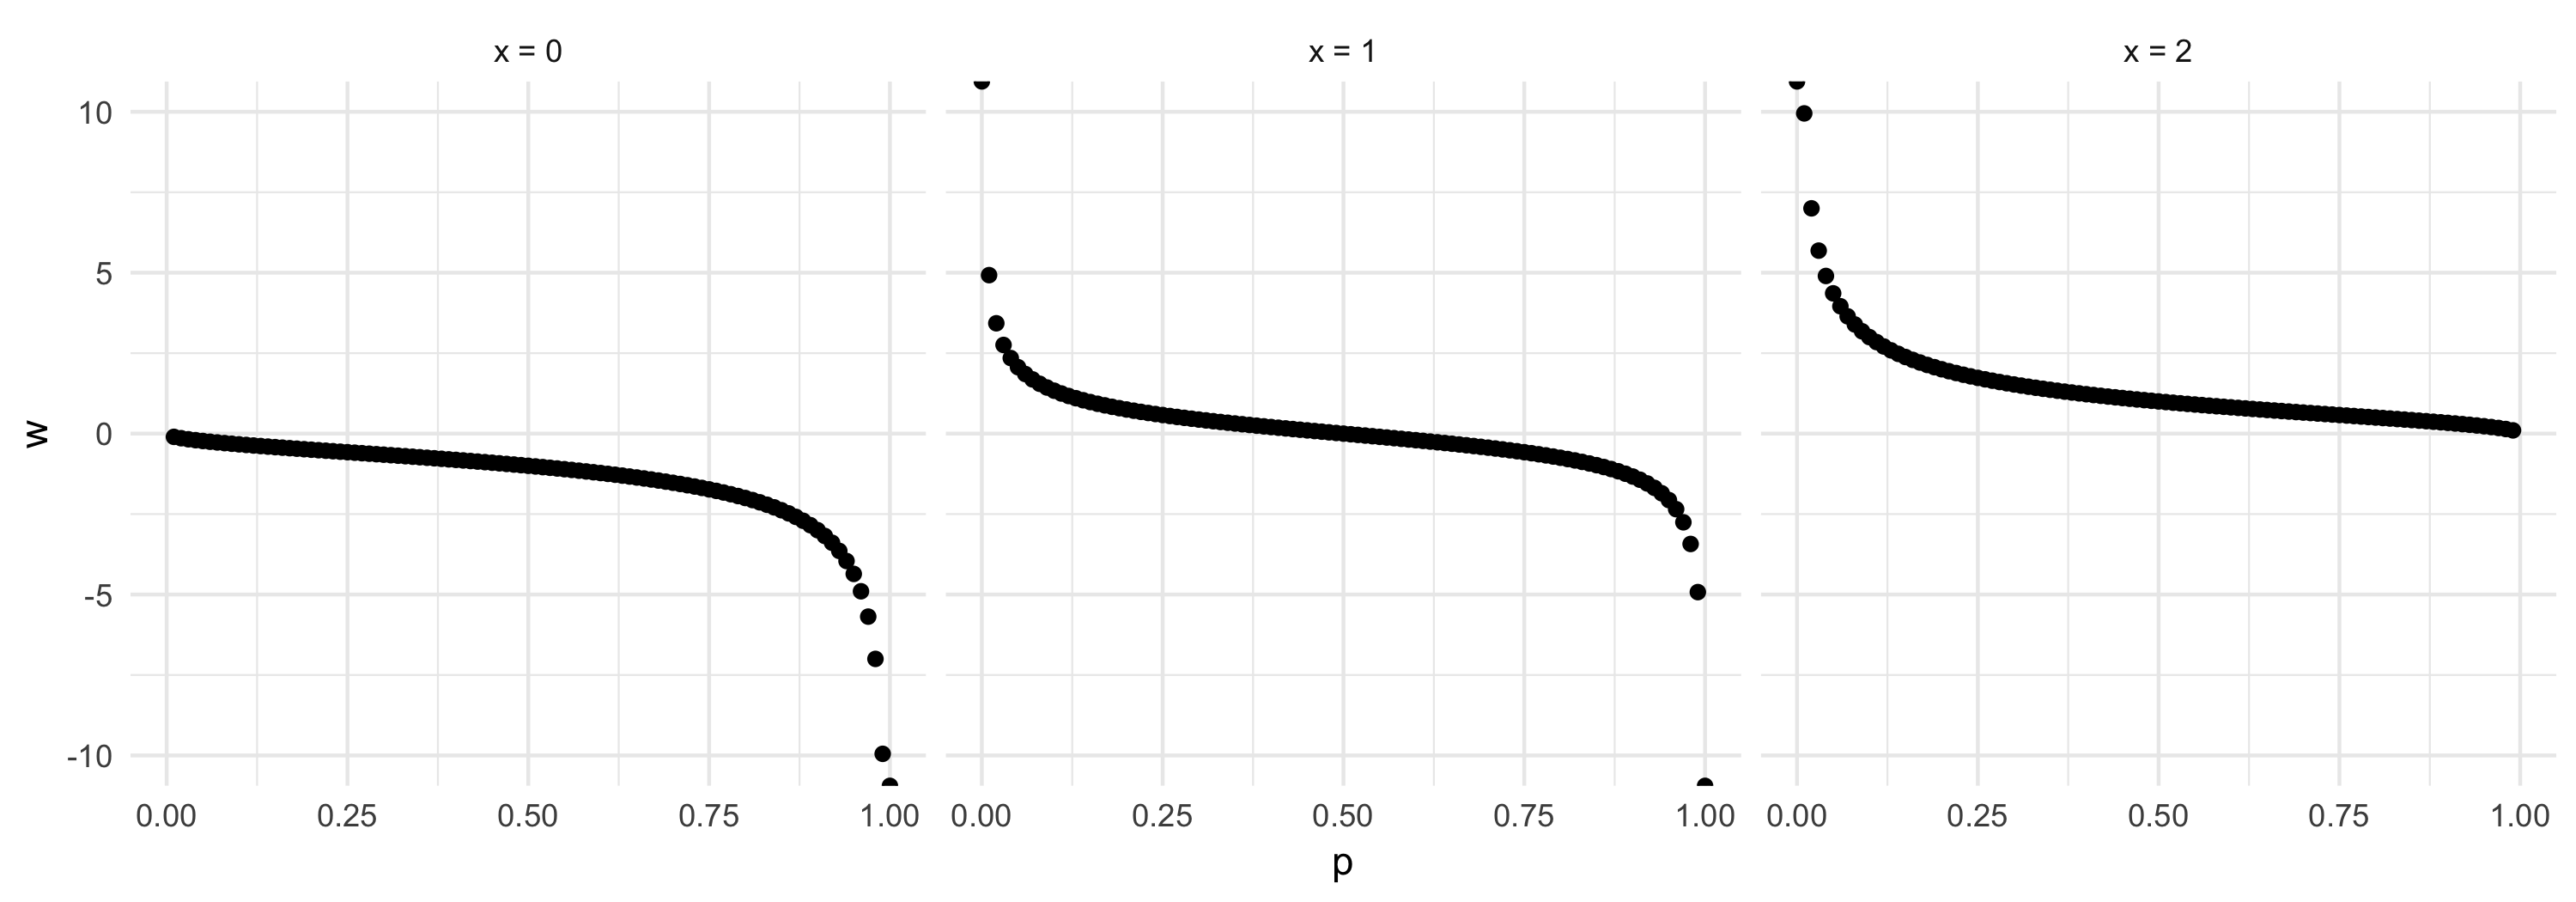
\includegraphics{fig/2_p_vs_w.png}
\caption{\label{fig:p-vs-w}Allelic effect \(i\) as function of causal allele frequency \(p\) for different counts of causal allele in a patient (\(x = 0, 1, 2\)).}
\end{figure}

An interesting bit of this simulation is the residual effect \(e_j\). It depends directly on the heritability of the trait, which must be given by the user via the \texttt{h2} parameter. Then \(e_j\) is generated from a Normal distribution with mean of 0 and variance

\[ \frac{1}{h^2 - 1} \text{var} \left(\sum\nolimits_i w_{ij} u_i\right),\]

where \(w\) and \(u\) are the weight and effect sizes specified above. When all variance is due to genetics (\(h^2 = 1\)), \(e_j = 0\) for all the patients \(j\).

Lastly, a user can request a binary phenotype setting the \texttt{qualitative} option to \texttt{TRUE}. In this case, the user must also specify three additional parameters: the number of cases (\texttt{ncases}), the number of controls (\texttt{ncontrols}), and the prevalence of the trait (\texttt{prevalence}). With these parameters, \texttt{simulate\_phenotype()} takes the \texttt{ncontrols} samples with the lowest \(y\) as controls, and the \texttt{ncases} samples with the highest \(y\) as cases. However, \texttt{ncases} needs to be lower or equal than \texttt{prevalence} \(\times |y|\), where \(|y|\) is the total number of samples in the GWAS experiment. This ensures that only the most extreme samples (as defined by the prevalence and the qualitative simulation) are cases.

\hypertarget{martini-ui}{%
\subsection{Interface, documentation and quality assurance}\label{martini-ui}}

Last, but not least, \emph{martini} includes the two main groups of functions required to run SConES. The first group involves the creation of the SNP networks, which were described in detail in Section \ref{methods:snp-network}. They are the \texttt{get\_GS\_network()}, to obtain a network that relates the SNPs based on genomic structure; \texttt{get\_GM\_network()} for a network that, on top of the previous one, relates SNPs mapped to the same gene; and \texttt{get\_GI\_network()} which, on top of the latter, relates SNPs mapped to genes that interact in a user provided list. The second important function is \texttt{scones()} which takes a GWAS dataset and a SNP network and runs SConES.

All functions exported by \emph{martini} have a \texttt{man} page, and hence information of the functions arguments, behavior and return value can be obtained via \texttt{help(fun)}. Accompanying examples and toy datasets are provided. Additionally, I wrote two vignettes to explain its basic behavior: one to run SConES (\href{https://www.bioconductor.org/packages/release/bioc/vignettes/martini/inst/doc/scones_usage.html}{\emph{Running SConES}}), and another to simulate network-based phenotypes (\href{https://www.bioconductor.org/packages/release/bioc/vignettes/martini/inst/doc/simulate_phenotype.html}{\emph{Simulating SConES-based phenotypes}}).

\emph{martini} was thoroughly subjected to unit tests via the \emph{testthat} package (Wickham \protect\hyperlink{ref-wickham_testthat:_2011}{2011}). At the moment of writing this text, \emph{martini} had a code coverage of 96\%.

\hypertarget{the-scones.nf-pipeline}{%
\section{\texorpdfstring{The \texttt{scones.nf} pipeline}{The scones.nf pipeline}}\label{the-scones.nf-pipeline}}

In addition to the changes implemented in \emph{martini}, I developed a ready-to-use computational pipeline that simplifies its usage: \texttt{scones.nf}. This pipeline just requires genotype data in PLINK binary file format and, when needed for the creation of a GM or GI network, a gene annotation file and a protein-protein interaction file. \texttt{scones.nf} is available on GitHub (\url{https://github.com/hclimente/gwas-tools}). In terms of function, the difference with vanilla \emph{martini} is that it performs an exhaustive grid-search to optimize both \(\lambda\) and \(\eta\), as opposed to \emph{martini}'s single grid search step. In the latter, both parameters explore the same range of values, which is calculated from the association scores \(c\) (e.g.~SKAT score). Specifically, it creates a linearly spaced n-component vector (n = 10 by default) between \(\lfloor \log_{10} \min(c) \rfloor\) and \(\lceil \log_{10} \max(c) \rceil\), then explores its powers of 10. On the other hand \texttt{scones.nf} makes the grid search finer, because it explores the grid in an iterative way. After the first exploration, identical to the one just described, the best \(\lambda\) and \(\eta\) according to some selection criterion are picked. Then it creates a new hyperparameter space, ranging from \(\log_{10}(\text{best } \lambda) - \Delta\) to \(\log_{10}(\text{best } \lambda) + \Delta\), where \(\Delta = 0.2(\log_{10}\max{(\text{explored }\lambda)}- \log_{10} \min{(\text{explored }\lambda)})\). The final \(\lambda\) and \(\eta\) are chosen using the same procedure on this new grid. Prior to these improvements, \texttt{scones.nf} was not able, in some instances, to recover the best solution, returning a trivial solution instead.

\hypertarget{conclusions}{%
\section{Conclusions}\label{conclusions}}

In this chapter I introduced \emph{martini} and the \texttt{scones.nf} pipeline. Jointly, they make SConES easily applicable to any GWAS dataset. Specially, they provide a wider range of options to the user in terms of how to measure the association between the genotypes and the phenotype, and how to select SConES hyper-parameters. Thanks to these improvements, we were able to obtain the SConES results presented in Chapter \ref{genesis}. Additionally, we provide a network-based phenotype simulation framework. \emph{martini} (Climente-González and Azencott \protect\hyperlink{ref-martini}{2019}) is available in Bioconductor (\url{https://www.bioconductor.org/packages/martini}); \texttt{scones.nf} is available on GitHub (\url{https://github.com/hclimente/gwas-tools}).

However, \emph{martini} and SConES still present shortcomings with regards to hyper-parameter selection (Sections \ref{results-benchmark} and \ref{genesis-issues}). As we note, SConES solutions were unstable despite using \emph{consistency} for model selection. This requires further examination. Additionally, when applied to GENESIS the selected solutions did not use the protein-protein interaction network, but other methods did. Although this is, to some extent, expected in that dataset, it does not inform much about the biology of the disease. In other words, in this case, SConES should be more tolerant to including unassociated SNPs in order to interconnect subnetworks of strongly associated SNPs. Hence, different parameters (lower values of \(\lambda\)) might relax the connectivity constraints enough to capture biological mechanisms more broadly. In this regard, it would be promising to use topological measures as scores for hyperparameter selection, for instance favoring settings that lead to densely interconnected networks. In this vein, it also is worth further exploring SigMod (Liu et al. \protect\hyperlink{ref-liu_sigmod:_2017}{2017}) a modification of SConES described in Section \ref{methods:methods}. While SConES penalizes selecting SNPs with many outbound edges and does not account for inbound edges, SigMod favours SNPs with many inbound edges, while disregarding outbound edges.

Lastly, I would like to explore SNP networks beyond the ones proposed in the original manuscript (Section \ref{methods:snp-network}). As I described in Section \ref{intro-interpretability}, and will deepen in Chapter \ref{epi-snp2gene}, there are multiple ways of relating SNPs to a function, and hence to build SNP networks. One compelling idea is to build a SNP network that reflects the 3D structure of the genome. Another opportunity for development involves encoding the LD relationship between the SNPs in the network, by tuning the edge weights. This would allow to either favor the selection of LD blocks (large LD implies large edge weight), or favor the selection of independent, associated SNPs (large LD implies small edge weight). These networks are very complex, involving hundreds of thousands of nodes and tens of millions of edges. In this regard, the ability of SConES to efficiently handle such networks enables this research and motivates working on solving the aforementioned issues.

\hypertarget{epi-snp2gene}{%
\chapter{Boosting interpretability and statistical power in epistasis detection by using prior biological knowledge}\label{epi-snp2gene}}

The contents of this chapter are based on \emph{Diane Duroux, Héctor Climente-González, Lars Wienbrandt, David Ellinghaus, Chloé-Agathe Azencott and Kristel Van Steen}, Boosting interpretability and statistical power in epistasis detection by using prior biological knowledge (manuscript in preparation). Parts of this work were presented in IGES 2019 in the poster \emph{Diane Duroux, Héctor Climente-González, Lars Wienbrandt, David Ellinghaus, Chloé-Agathe Azencott and Kristel Van Steen}, Improving efficiency in epistasis detection with a gene-based analysis using functional filters.

\begin{chapabstract}{Abstract:}
Detecting epistatic interactions at the gene level is essential to understanding the biological mechanisms of complex diseases. Unfortunately, genome-wide interaction association studies (GWAIS) involve many statistical challenges that make such detection hard. This chapter considers three steps to analyze the conversion of SNP-SNP interactions into a gene-gene network through the integration of biological knowledge. First, we investigate the use of known gene-gene interactions to focus on the most promising gene-pairs. Second, we explore several functional SNP-to-gene mappings to map SNPs to these gene interactions, including expression quantitative trait loci (eQTL) and chromatin-based, and filter the GWAIS data accordingly. Third, we integrate SNP-pairs statistics into gene-pairs statistics using the adaptive truncated product method (ATPM). ATPM does not require parameters or a known null distribution, and it is fast to compute. We apply different variants of these three steps to a GWAS inflammatory bowel disease (IBD) dataset, and compare the results. Overall, knowledge integration decreases the number of tests performed, reducing computational time and boosting statistical power, and provides interpretability. We validate through a permutation analysis that type I error is under control. The different protocols produce different results, which highlight different mechanisms implicated in IBD while, at the same time, overlapping with the known biology of the disease. Using eQTLs results in more interactions than the standard approach, where all possible SNP pairs are investigated and SNPs are mapped to genes based on their position on the genetic sequence, albeit fewer significant gene-pairs. This pipeline not only detects interactions at the gene level, but also gives a global visualization that identifies neighbors, hubs and highly connected substructures.
\end{chapabstract}
\vskip 0.2in
\begin{chapabstract}{Résumé :}
La d\'etection d'interactions \'epistatiques entre g\`enes est essentielle \`a 
la compr\'ehension des m\'ecanismes des maladies complexes. Malheureusement, 
les \'etudes d'association d'interactions g\'enome entier (GWAIS) posent de 
nombreux d\'efis statistiques qui rendent cette d\'etection difficile. Ce 
chapitre consid\`ere trois \'etapes pour analyser la conversion 
d'interactions SNP-SNP en un r\'eseaux de g\`enes, \`a travers l'int\'egration 
de connaissances biologiques. Tout d'abord, nous nous int\'eressons \`a 
l'utilisation d'interactions g\`ene-g\`ene connues afin de nous limiter aux 
paires de g\`enes les plus prometteuses. Deuxi\`emement, nous \'etudions 
plusieurs correspondances fonctionnelles entre SNPs et g\`enes, bas\'ees 
entre autre sur les loci r\'egulant l'expression (eQTL) ou les contacts de 
chromatine, que nous utilisons aussi pour filtrer les donn\'ees. 
Troisi\`emement, nous proposons de d\'eriver, des statistiques obtenues pour 
des paires de SNPs, une statistique pour une paire de g\`enes, par une 
m\'ethode de produit tronqu\'e adaptative (ATPM). L'ATPM ne requiert ni de 
fixer des param\`etres, ni de connaître la distribution nulle, et peut 
\^etre calcul\'ee efficacement. Nous appliquons diff\'erentes variantes de ces 
trois \'etapes \`a un jeu de donn\'ees GWAS des maladies chroniques 
inflammatoires de l'intestin (MICI), et comparons les r\'esultats obtenus. 
L'int\'egration de connaissances    extit{a priori} permet de r\'eduire le 
nombre de tests statistiques \`a effectuer, ce qui r\'eduit les temps de 
calculs et augmente la puissance statistique. Elle facilite aussi 
l'interpr\'etation des r\'esultats. Une analyse par permutations nous permet 
de valider que l'erreur de type I est bien contr\^ol\'ee. Diff\'erents 
protocoles produisent des r\'esultats diff\'erents, qui mettent en lumi\`ere 
diff\'erents m\'ecanismes impliqu\'es dans les MICI, tout en coïncidant avec 
des m\'ecanismes d\'ej\`a connus de ces maladies. L'utilisation de 
correspondances SNPs identifi\'es dans des eQTLs permet d'obtenir plus 
d'interactions SNP-SNP que l'approche standard, mais moins de paires de 
g\`enes significatives. Notre pipeline permet non seulement de d\'etecter 
des interactions entre g\`enes, mais aussi de les visualiser dans un 
r\'eseau global, et d'identifier voisinages, hubs, et structures fortement 
interconnect\'ees.
\end{chapabstract}

\hypertarget{introduction-2}{%
\section{Introduction}\label{introduction-2}}

In this chapter we study the detection of gene-level epistasis from
SNP-level epistasis to improve the interpretability of GWAIS. Our
analysis compares ways of converting statistical epistasis at the SNP
level into a gene-based statistical epistasis network. First, we
investigate different functional filters (Ma, Keinan, and Clark \protect\hyperlink{ref-ma2015biological}{2015}) and
SNP-to-gene mapping functions.
Second, as a bijectivity issue arises because a SNP can be mapped on
several genes, we investigate the use of current knowledge on gene-gene
interaction to focus on the most promising gene-pairs. We study whether
the epistatic interactions driving the phenotype are likely to be
currently in existing databases. Third, we used the adaptive truncated
product method to estimate gene-pairs significance.

\hypertarget{materials-and-methods}{%
\section{Materials and methods}\label{materials-and-methods}}

\hypertarget{snp2gene-qc}{%
\subsection{Dataset and initial quality control}\label{snp2gene-qc}}

We investigated the IIBDGC dataset, described in
Section \ref{iibdgc-dataset}, whose large sample size helps to overcome the
issue of reduced statistical power common in GWAIS.
We performed a quality control as in Ellinghaus et al. (\protect\hyperlink{ref-ellinghaus_analysis_2016}{2016}), reducing the
number of SNPs from 196,524 to 130,071.

The IIBDGC dataset aggregates different cohorts, and contains
confounding population structure (Section \ref{pop-structure}). PLINK
(Purcell et al. \protect\hyperlink{ref-purcell2007plink}{2007}) cannot take covariates in the logistic regression used to
detect epistasis (Section \ref{methods:snp-epistasis}). In consequence, we adjusted
phenotypes to account for population structure using the top 7 principal
components as in Ellinghaus et al. (\protect\hyperlink{ref-ellinghaus_analysis_2016}{2016}). Essentially, we derive adjusted
phenotypes from the logistic regression model by subtracting model-fitted
values from observed phenotype values (i.e.~response residuals).

\hypertarget{methods:pipeline}{%
\subsection{Gene interaction detection procedure}\label{methods:pipeline}}

As we describe below, we applied four different functional filters to
the dataset. The functional filter used known interactions between
genes, and the three different ways of mapping SNPs to genes described in Section
\ref{intro-interpretability}, and hence, to
these interactions. In essence, in each of the filtered datasets we only tested
the interactions between SNPs which can be mapped in a particular way to
a pair of interacting genes. The resulting four datasets
(including an unfiltered dataset) were analyzed separately. For
convenience, we will refer to their associated analyses using the terms
\emph{Standard}, \emph{physical}, \emph{eQTL} and \emph{chromatin}. For each dataset, the
entire pipeline described below is applied and the four obtained outputs
are subsequently compared. An overview of the whole pipeline is
available in Figure \ref{fig:pipeline}.



\begin{figure}
\centering
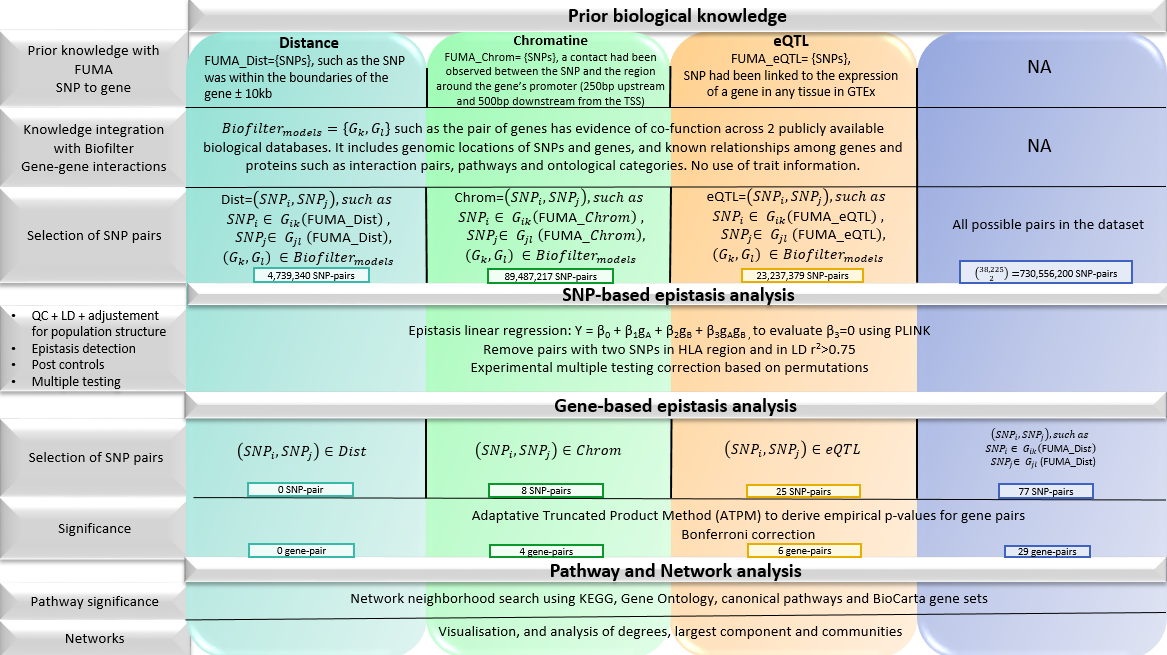
\includegraphics{fig/pipeline2.PNG}
\caption{\label{fig:pipeline}Overview of the gene-gene interaction detection procedure (from Duroux et al. (\protect\hyperlink{ref-duroux_2019_iges}{2019})). The whole protocol is described in Section \ref{methods:pipeline}.}
\end{figure}

\hypertarget{methods:prefiltering}{%
\subsubsection{Functional SNP pre-filtering}\label{methods:prefiltering}}

The initial step of the protocol is a functional SNP pre-filtering,
which has three stages. First, we mapped the SNPs in the dataset to
genes using FUMA (Watanabe et al. \protect\hyperlink{ref-watanabe_functional_2017}{2017}). FUMA is a post-GWAS
annotation tool. Its SNP2GENE function takes GWAS summary statistics and
maps significant SNPs to genes according to both physical and functional
criteria specified by the user. We created an artificial input where
every SNP is significant in order to perform such mapping on all the
SNPs. We performed three SNP-gene mappings using SNP2GENE: physical,
eQTL and 3D chromatin interaction. In the physical mapping, we mapped a
SNP to a gene when the former was within the boundaries of the latter
\(\pm\) 10 kb. The eQTL mapping uses eQTLs obtained
from GTEx (GTEx Consortium \protect\hyperlink{ref-gtex_consortium_genetic_2017}{2017}). We mapped an eQTL SNP to its target gene when the
association P-value was significant in any tissue (\(\text{FDR} < 0.05\)).
Lastly, in the 3D chromatin interaction mapping, we mapped a SNP to a
gene when a contact had been observed between the former and the region
around the latter's promoter (250 bp upstream and 500 bp downstream from
the transcription start site) in any of the Hi-C datasets included in
FUMA (\(\text{FDR} < 10^{-6}\)). The chromatin mapping might contain new,
undiscovered, regulatory variants which, as eQTL, regulate the expression
of a gene.

Second, after obtaining the SNP-to-gene mappings, we used Biofilter 2.4
(Pendergrass et al. \protect\hyperlink{ref-pendergrass_genomic_2013}{2013}) to obtain the candidate gene-pairs
subsequently investigated for epistasis evidence. Biofilter generates
pairs of genes with evidence of co-function across multiple publicly
available biological databases. It includes genomic locations of SNPs
and genes, as well as known relationships among genes and proteins such
as interaction pairs, pathways and ontological categories.
Notably, it does not use trait information.
Specifically, we considered only pairs of genes for which both genes
could be mapped, using any of the mappings, to a SNP in our GWAS
dataset. We used only gene pairs supported by evidence in at least 2
databases. When the two SNPs of a pair were located in the HLA region,
we removed the pair, as this complex genomic region is currently not
well understood. Additionally, we removed self-interactions, as
detection of within-gene epistasis requires special considerations and
is beyond the scope of this paper.

Lastly, we filtered the datasets again to explore exclusively
interactions between SNPs mapped to genes known to interact, according
to Biofilter. For that purpose we first converted the Biofilter
gene-pair models into SNP-pair models separately via each of the FUMA
SNP-gene mappings described above. Then, from these SNP pairs sets, we
built the four datasets enumerated above: one without any filter (\emph{Standard});
and one for each SNP to gene mapping (\emph{Physical}, \emph{eQTL},
\emph{Chromatin}). It is worth pointing out that SNP-pair models
were also built based exclusively on the corresponding mapping e.g.
\emph{physical} contains exclusively pairs of SNPs which can be associated to
pairs of genes via a physical mapping. This helps interpretability and
keeps the number of tested interactions under control.

\hypertarget{post-filtering-quality-control}{%
\subsubsection{Post-filtering quality control}\label{post-filtering-quality-control}}

Additional quality controls were performed on each of the four generated
datasets. As motivated in Gusareva and Van Steen (\protect\hyperlink{ref-gusareva_practical_2014}{2014}), only common variants
(\(\text{MAF} > 5\)\%) and in Hardy--Weinberg equilibrium (\(\text{P-value} > 0.001\)) are
considered. Also, we pruned SNPs that are in linkage equilibrium
(\(R^{2} > 0.75\)). Lastly all risk SNP described in Liu et al. (\protect\hyperlink{ref-liu2015association}{2015}) were
included.

\hypertarget{methods:snp-epistasis}{%
\subsubsection{SNP-level epistasis detection and multiple test correction}\label{methods:snp-epistasis}}

We used PLINK 1.9 to detect epistasis through a linear regression on the adjusted phenotypes:

\[Y = \beta_0 + \beta_1 g_A + \beta_2 g_B + \beta_3 g_A g_B,\]

where \(g_A\) and \(g_B\) are the genotypes under additive encoding for SNPs
A and B respectively; \(\beta_0\), \(\beta_1\), \(\beta_2\), \(\beta_3\), are
the regression coefficients. PLINK performs a statistical test to
evaluate if \(\beta_3 \neq 0\). Crucially, it only returns SNP-pairs
with a P-value lower than a specified threshold. We used the default
0.0001.

We only considered pairs of SNPs not in strong LD (\(R^{2}<0.75\)) and
that could be mapped to the corresponding SNP-model obtained from
Biofilter, with self-gene interactions removed (Section
\ref{methods:prefiltering}). This impacted the total number of
statistical tests.

To correctly account for multiple testing, the P-value threshold of
significance had to be dataset-dependent as the number of tested SNP
pairs changed from dataset to dataset (Section
\ref{methods:prefiltering}). We obtained the threshold through a
permutation analysis as in Hemani et al. (\protect\hyperlink{ref-hemani_detection_2014}{2014}). In essence,
for each dataset, we permuted the phenotypes 400 times and measured SNP
association as above. This produced a null distribution of the extreme
P-values for this number of tests given the LD structure. For each
dataset, we took the most extreme P-value from each of the 400
permutations and set the threshold for 5\% family-wise error rate
(FWER) to be the 95\% percentile of these most extreme P-values.

\hypertarget{methods:gene-networks}{%
\subsubsection{From SNP-level to gene-level epistasis}\label{methods:gene-networks}}

Next we converted SNP pairs into gene-pairs using their respective FUMA
and Biofilter mappings (Section \ref{methods:prefiltering}).
The exception was the \emph{Standard}
dataset, where SNPs are physically mapped to genes, and no Biofilter
restriction on which pairs of genes can interact was applied. Still,
self-interactions were removed.

Then, we computed gene-level statistics from the respective SNP-level
statistics of the involved SNPs. In this regard, all \(N\) pairs of SNPs
mapped to a gene pair are taken as a set of tests on the same global
null hypothesis \(H_{0i}\), where \(i=1,2,\dots ,N\). Zaykin et al. (\protect\hyperlink{ref-zaykin2002truncated}{2002})
developed the truncated product method (TPM) as a method to combine
P-values on a same global hypothesis. It does so by computing the
statistic \(W(\tau)=\prod_{i=1}^{N} p_i^{I(p_{i}\le\tau)}\) where
\(I(\cdot)\) is the indicator function and \(\tau\) is the truncation point.
A P-value \(\hat{s}(\tau)\) can be the estimated for a given \(W(\tau)\).
TPM was interesting since we did not not have
P-values for every SNP pair but for the most strongly associated ones
only (Section \ref{methods:snp-epistasis}). However, TPM requires setting the
truncation point \(\tau\), a parameter that is arbitrary and might be
gene-pair specific. On top of that, the null distribution of \(W(\tau)\)
is unknown when P-values are correlated, as is the case. To solve these
problems the adaptive truncated product method (ATPM) was proposed
(Sheng and Yang \protect\hyperlink{ref-sheng2013adaptive}{2013}). ATPM explores different \(\tau\), choosing the one
that produces the minimum P-value \(\hat{s}(\tau)\). We estimated the
distribution of the ATPM using permutations as in Ge, Dudoit, and Speed (\protect\hyperlink{ref-ge2003resampling}{2003}).
Specifically, we created \(B = 999\) permuted datasets by permuting the
phenotype vector. Based on the \(b^{th}\) permuted dataset,
\(1 \leq b \leq B\), we perform the N individual tests. We used three
values for \(\tau\) (0.001, 0.01, 0.05) and set the significance level
\(\alpha=0.05\). The specific procedure goes as follows:

\begin{enumerate}
\def\labelenumi{\arabic{enumi}.}
\item
  For each gene-pair in the output of the original data analysis,
  based on \(p{_1}^{(b)},...,p{_N}^{(b)},1\le b\le B\), calculate the
  truncated product statistics for each candidate truncation threshold
  for the original data and B permuted datasets.
\item
  Use Ge's algorithm to obtain the estimated P-value
  \(\hat{s}_{k}^{b}=\frac{\sum_{l=0}^B I(W(\tau_k)_b \geq W(\tau_k)_l)}{B+1}\),
  \(1 \le k \le 3\), \(0 \le b \le B\)
\item
  Calculate \(M{_b}=min_{1 \le k \le 3}\hat{s}_{k}^{b}\)
\item
  The adjusted P-value for the adaptive truncated product statistic
  \(M\) is estimated as
  \(P_{minP^{(b)}}=\frac{\sum_{b=0}^B I(M \geq M_b)}{B+1}\).
\item
  We reject the joint null hypothesis if the adjusted P-value is
  smaller than the global significance level \(\alpha\).
\end{enumerate}

\hypertarget{results}{%
\section{Results}\label{results}}

\hypertarget{type-i-error}{%
\subsection{Type I error}\label{type-i-error}}

The ``multi-stage'' nature of the protocol presented in Section
\ref{methods:pipeline} required controlling the type I error. For
that purpose, we performed 1,000 permutation analyses for each of the
four datasets, permuting the phenotypes and running the entire protocol
to detect significant gene pairs. When at least one significant
gene-pair is observed in a permutation, that permutation is considered a
false positive (FP). This allowed to compute the type I error rate as
\(\frac{ \text{\# FP}}{1000}\). We observed that the type I error was
under control for all four datasets (3.6\%, 3.7\%, 6.1\%, and 3.9\% for \emph{Standard},
\emph{Physical}, \emph{Chromatin}, and \emph{eQTL}, respectively).

\hypertarget{results-power-gain}{%
\subsection{Chromatin contacts map more SNPs per gene than other mappings}\label{results-power-gain}}

We considered three procedures to map SNPs to their gene, as a proxy for
their link to functionality (Section
\ref{methods:prefiltering}): \emph{physical}, \emph{eQTL} and \emph{chromatin}.
\emph{Chromatin} produced the largest number of mappings (2,394,589), an
order of magnitude more than \emph{eQTL} (411,120) and \emph{physical} (174,879)
(Table \ref{tab:datasets-snps}). Similarly, \emph{chromatin} has
the largest number of SNPs mapped to an individual gene, followed by \emph{eQTL} and
\emph{physical} (Figure \ref{fig:snps-per-mapping}A). Nonetheless,
different genes had very unequal contributions from each of the mappings
(Figure \ref{fig:snps-per-mapping}B). This is consistent with
the striking differences between the ranking of genes according to the number of
SNPs mapped on them (Figures \ref{fig:snps-per-mapping}C, D and E):
in general, the genes with the most SNPs mapped using the eQTL mapping had
relatively few SNPs mapped in the chromatin mapping, and viceversa.



\begin{figure}
\centering
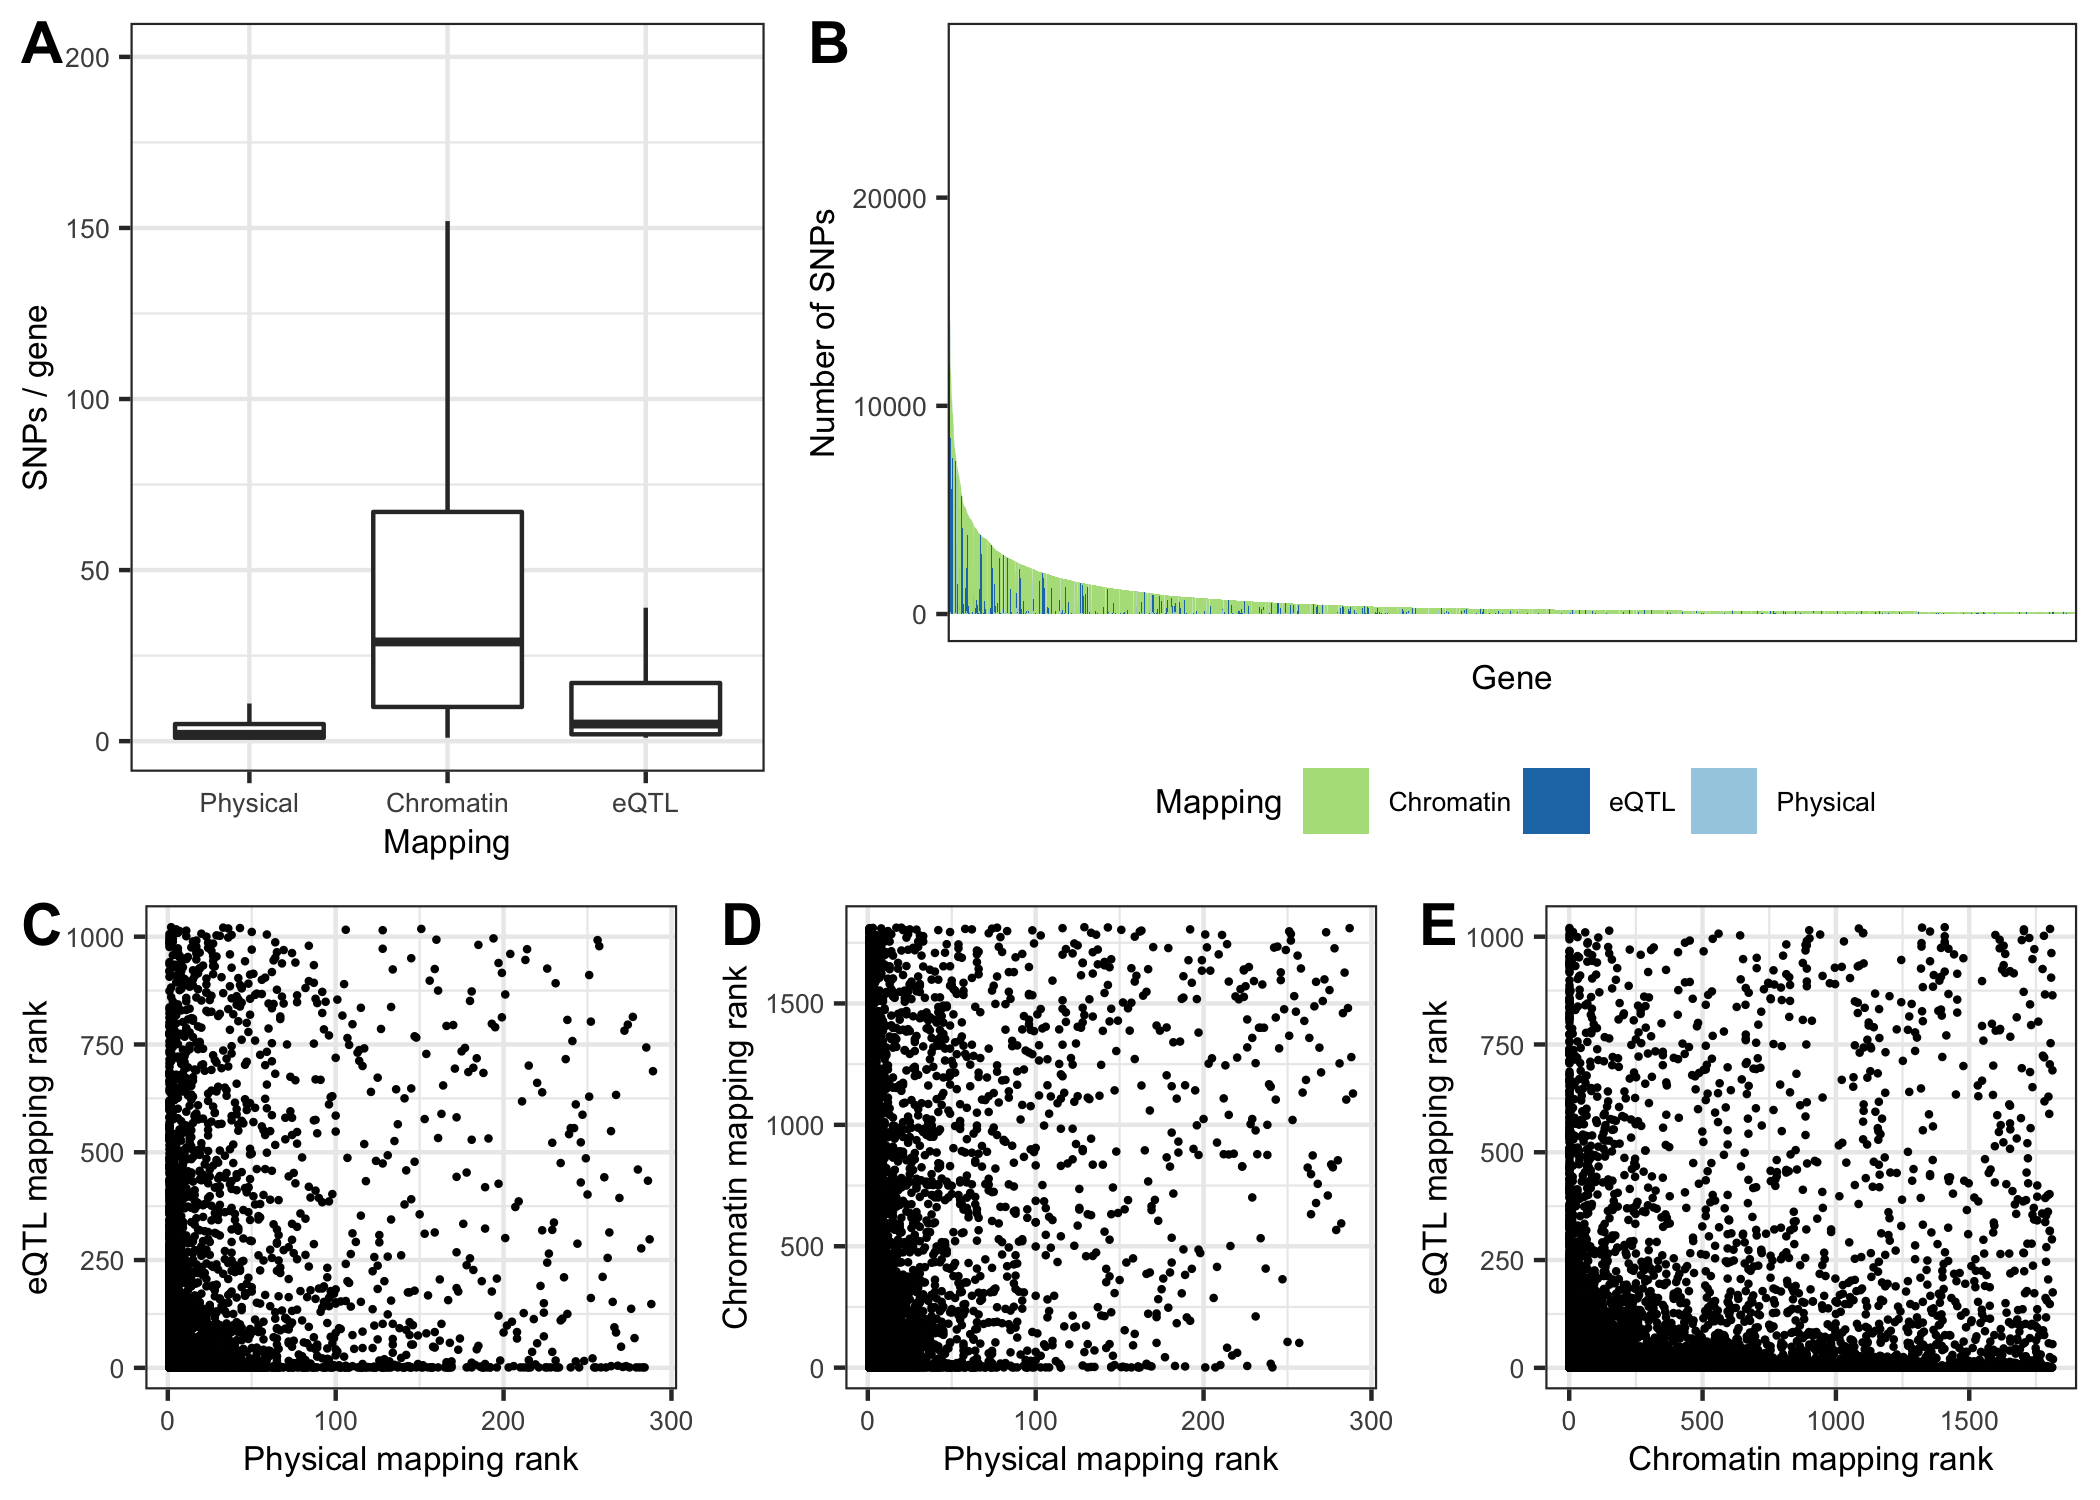
\includegraphics{fig/mappings_per_gene.png}
\caption{\label{fig:snps-per-mapping}\textbf{(A)} Number of SNPs per gene for each of the three mappings described in Section \ref{methods:prefiltering}. Outliers are not displayed to facilitate visualization. \textbf{(B)} Ranking of genes with most SNPs mapped using any of the mappings, colored by mapping. Only genes with more than 100 SNPs mapped to it are displayed. \textbf{(C,D,E)} Comparison between the rank of each gene according to the number of SNPs mapped to it using each mapping.}
\end{figure}

The number of mappings is directly linked the number of SNPs and
interactions tested per dataset (Table \ref{tab:datasets-snps}). As it can be
observed, restricting our search exclusively to Biofilter-plausible interactions
leads to an increase in statistical power with respect to the \emph{Standard}
protocol. Specifically, the number of tests are between 1 and 2 orders of
magnitude smaller.

\begin{table}

\caption{\label{tab:datasets-snps}Properties of the different SNP-gene mappings and the filtered datasets.}
\centering
\begin{tabular}[t]{lllll}
\toprule
 & Standard & Physical & Chromatin & eQTL\\
\midrule
\rowcolor{gray!6}  \# SNPs & 38225 & 16417 & 30146 & 16652\\
\# SNP-gene mappings & NA & 1.7e+05 & 2.4e+06 & 4.1e+05\\
\rowcolor{gray!6}  \# tests & 7.2e+08 & 4.6e+06 & 8.9e+07 & 2.2e+07\\
\bottomrule
\end{tabular}
\end{table}

\hypertarget{the-physical-protocol-does-not-recover-any-snp-interaction}{%
\subsection{\texorpdfstring{The \emph{Physical} protocol does not recover any SNP interaction}{The Physical protocol does not recover any SNP interaction}}\label{the-physical-protocol-does-not-recover-any-snp-interaction}}

We searched SNP epistasis in the four datasets (Section
\ref{methods:snp-epistasis}). The different epistatic SNP-SNP networks are
described on Table \ref{tab:snp-network} and Figure
\ref{fig:snp-networks}. Strikingly, while the \emph{Standard} protocol generated the
largest network (55 nodes), the \emph{eQTL} one was the largest by number of
interactions (64). The \emph{Physical} protocol produced no significant pairs.

\begin{table}

\caption{\label{tab:snp-network}Properties of the SNP networks from the different datasets.}
\centering
\begin{tabular}[t]{lllll}
\toprule
 & Standard & Physical & Chromatin & eQTL\\
\midrule
\rowcolor{gray!6}  \# significant pairs & 57 & 0 & 19 & 64\\
\# nodes & 55 & 0 & 20 & 46\\
\rowcolor{gray!6}  \# connected components & 12 & NA & 5 & 6\\
Size of the largest component & 25 & NA & 11 & 17\\
\rowcolor{gray!6}  Average degree & 2.07 & NA & 1.9 & 2.78\\
\bottomrule
\end{tabular}
\end{table}



\begin{figure}
\centering
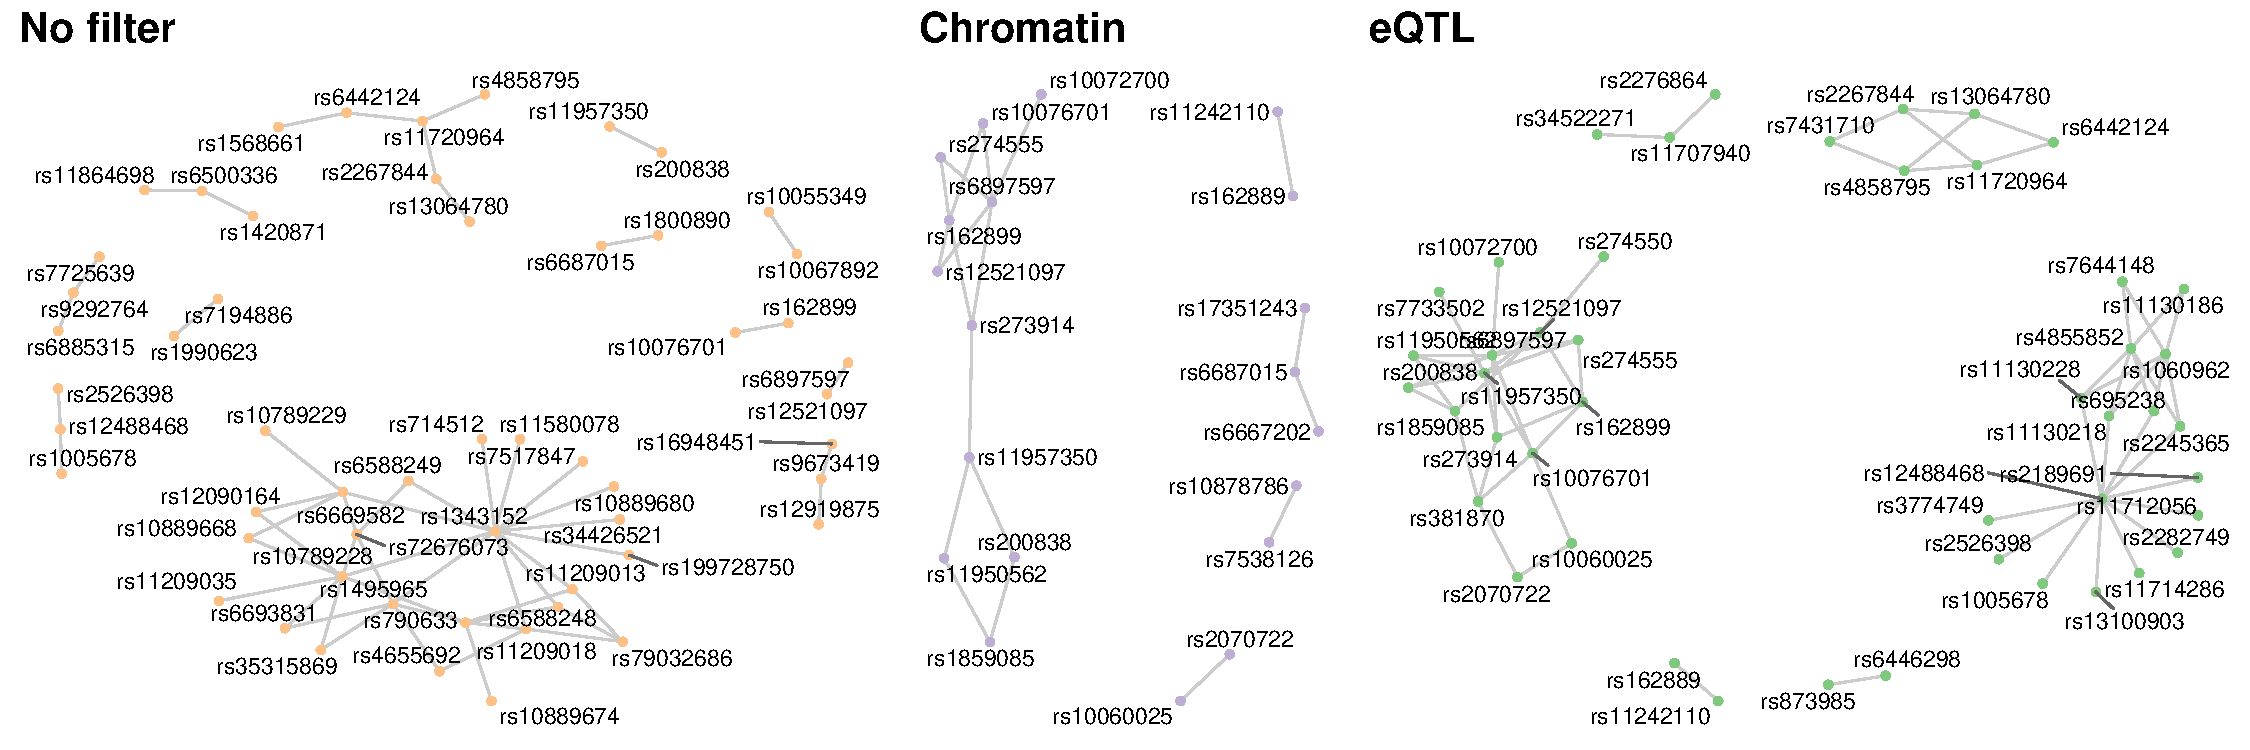
\includegraphics{fig/snp_networks.pdf}
\caption{\label{fig:snp-networks}SNP-level epistasis networks for \emph{Standard} (orange), \emph{eQTL} (green), and \emph{Chromatin} (violet) (Sections \ref{methods:prefiltering} and \ref{methods:snp-epistasis}). The \emph{Physical} dataset is absent, as no SNP pairs were significant.}
\end{figure}

\hypertarget{results:gene-networks}{%
\subsection{Gene-level network}\label{results:gene-networks}}

We converted the aforementioned SNP-pair networks into gene-pair epistasis
networks, estimating their significance through ATPM (Section
\ref{methods:gene-networks}). Most of the SNP-pairs mapped to exclusively one
gene pair in \emph{eQTL} and \emph{Standard}, removing possible sources of ambivalence
(Figure \ref{fig:sign-snps-per-gene-and-viceversa}A). That was
not the case under the chromatin mapping, where it was more common for the same
SNP pair to map to different gene pairs. We then compared the relationship
between significant gene-pairs and the number of significant SNP pairs that map
to them (Figure \ref{fig:sign-snps-per-gene-and-viceversa}B).
Interestingly, most significant gene pairs are supported by
relatively small number of SNPs: either few in number, or few with respect to
the total number of SNP pairs for that gene pair.



\begin{figure}
\centering
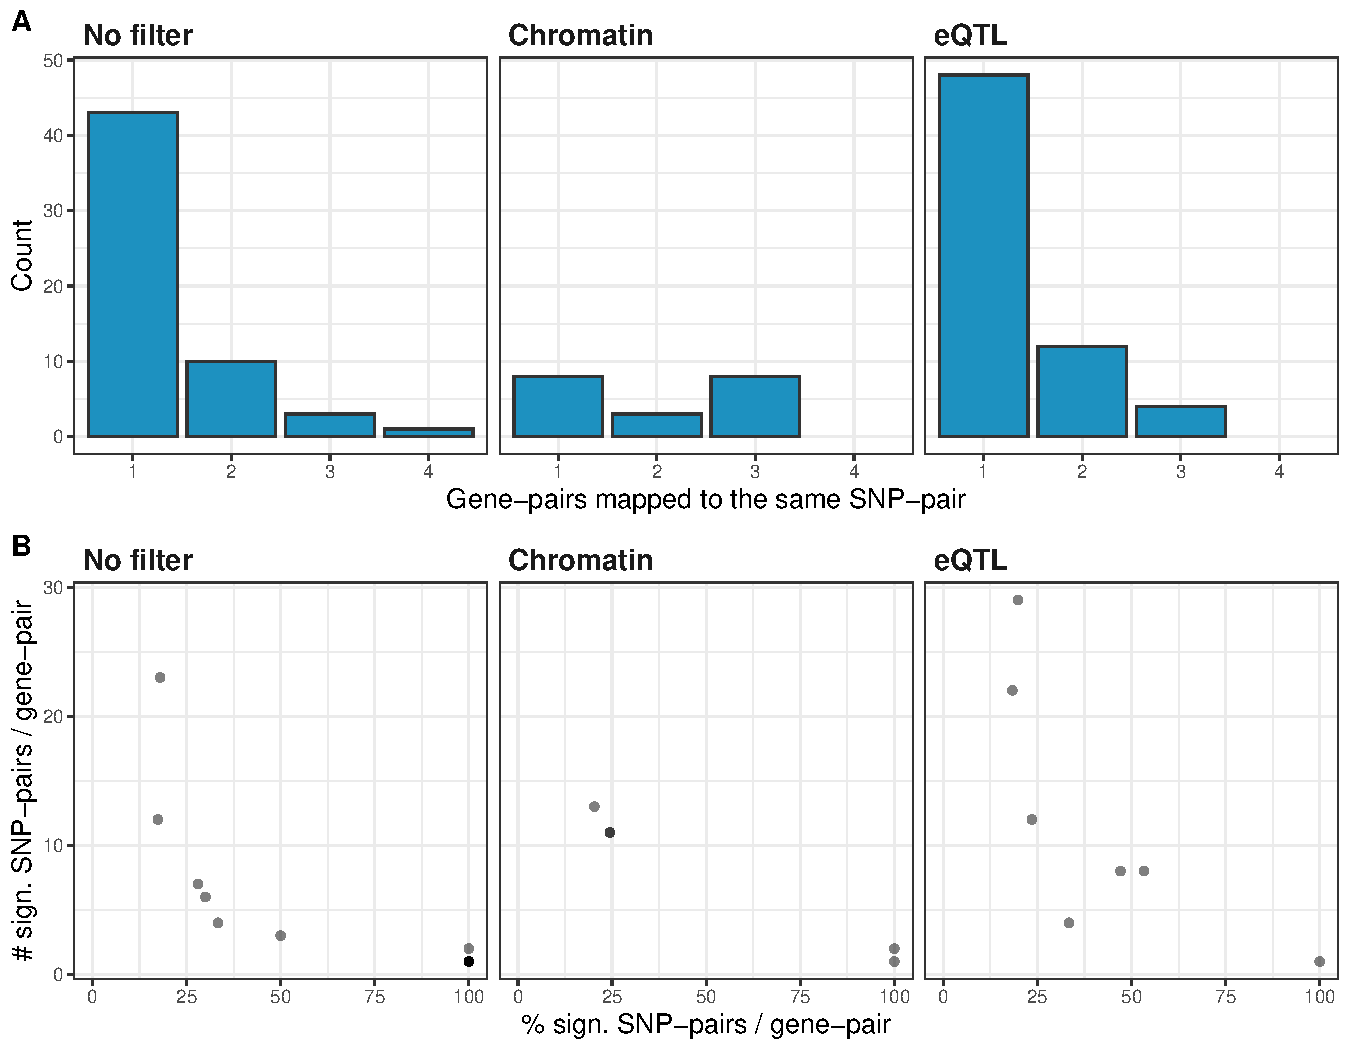
\includegraphics{fig/sign_snps_per_gene_and_viceversa.pdf}
\caption{\label{fig:sign-snps-per-gene-and-viceversa}Relationship between the number of significant SNP pairs and of significant gene pairs. \textbf{(A)} Histogram of the number of significant gene pairs mapped to the same SNP pair. \textbf{(B)} Relationship between the total number of SNP pairs mapped to the same gene pair (y-axis), and the percentage of all significant SNP-pairs between all the SNP-pairs mapped to the same gene (x-axis). Data points are semi-transparent, so multiple points stacked result in a darker shade.}
\end{figure}

We built an epistatic gene network from the significant gene pairs
(Methods \ref{methods:gene-networks}), shown in Figure \ref{fig:gene-networks}
and Table \ref{tab:gene-networks-stats}. Overall, the \emph{Standard} protocol still
produces the largest network, and contains more connected components and
significant gene-pairs. On the other hand, \emph{Chromatin} and \emph{eQTL} mappings
produce similar networks in terms of sizes, number of gene-pairs and
connected components. However, both \emph{Chromatin} and \emph{eQTL}'s networks are
notably smaller than \emph{Standard}'s (11 and 10 nodes versus 29,
respectively).

\emph{Standard}'s nodes are proportionally more clustered in
connected components, while most \emph{eQTL} and \emph{Chromatin}'s connected
components are composed of only a pair of genes. Although this might
reveal the affection of a common mechanism, it is likely a result of the
overlap in the genome of multiple genes, which are mapped to highly
overlapping sets of SNP.

\begin{table}

\caption{\label{tab:gene-networks-stats}Properties of the gene networks from the different datasets.}
\centering
\begin{tabular}[t]{lllll}
\toprule
 & Standard & Physical & Chromatin & eQTL\\
\midrule
\rowcolor{gray!6}  \# significant pairs & 26 & 0 & 5 & 7\\
\# nodes & 29 & 0 & 10 & 11\\
\rowcolor{gray!6}  \# connected components & 8 & NA & 5 & 5\\
Size of the largest component & 6 & NA & 2 & 3\\
\rowcolor{gray!6}  Average degree & 1.79 & NA & 1 & 1.27\\
\bottomrule
\end{tabular}
\end{table}



\begin{figure}
\centering
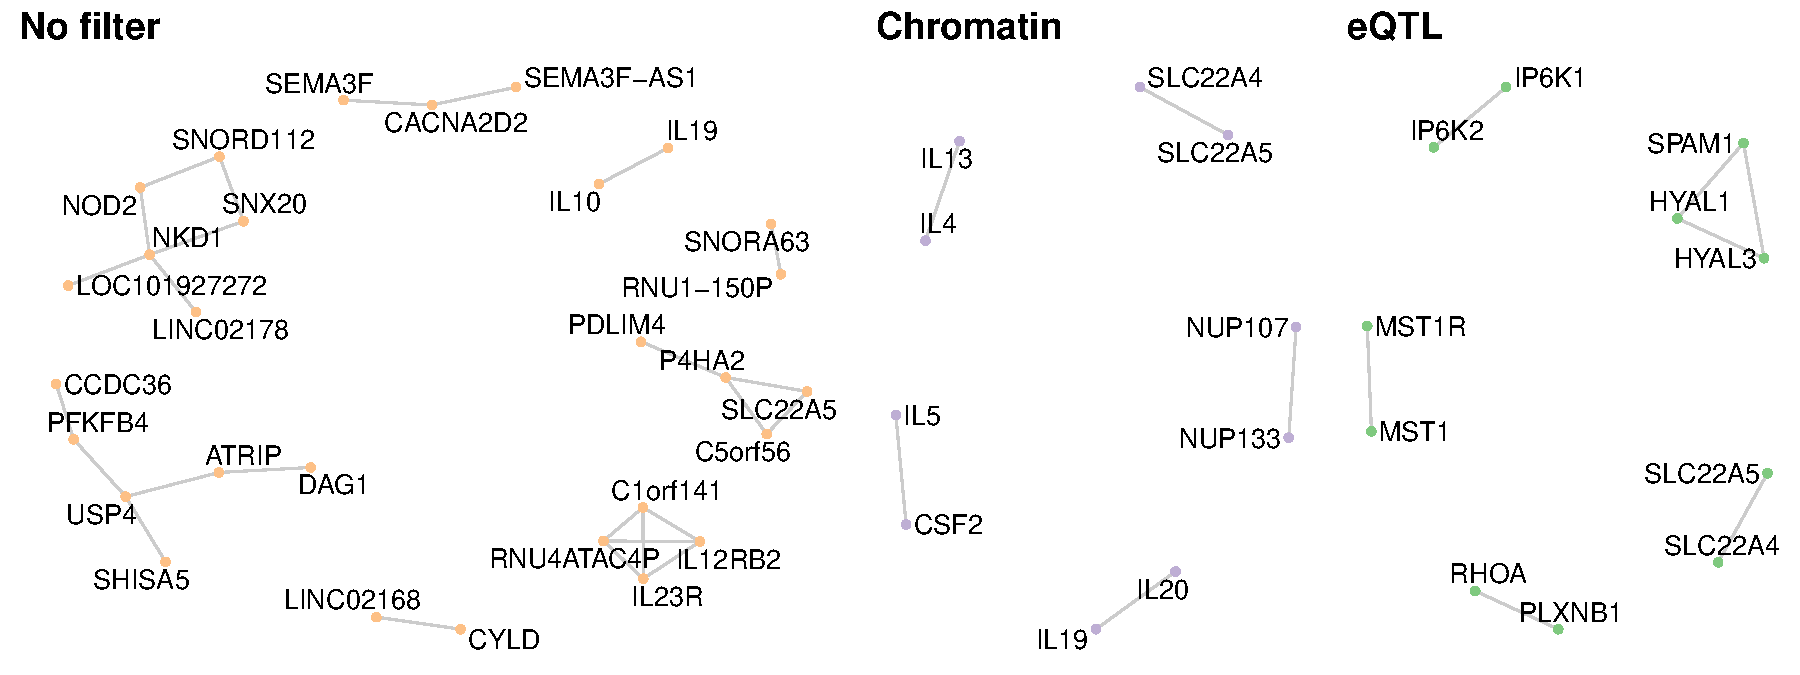
\includegraphics{fig/gene_networks.pdf}
\caption{\label{fig:gene-networks}Gene-level epistasis networks for \emph{Standard} (orange), \emph{eQTL} (green), and \emph{Chromatin} (violet) (Section \ref{methods:prefiltering}).}
\end{figure}

A hub is node with a number of links that greatly exceeds the average.
For this application, we define a hub as a node having a degree strictly
superior to three. Only the \emph{Standard} process contains such hubs: \emph{P4HA2},
\emph{NKD1}, \emph{RNU4ATAC4P}, \emph{C1orf141}, \emph{IL12RB2}, \emph{IL23R} and \emph{USP4}.

Jointly, 38 significant gene pairs are involved in at least one method,
involving 46 unique genes. Seven chromosomes are involved in epistasis.
Notably, 39\% of the epistatic genes are located in chromosome 3 and 22\%
in chromosome 10.

\hypertarget{results-ibd-soa}{%
\subsection{\texorpdfstring{\emph{Chromatin} and \emph{Standard} mappings partially replicate previous studies on IBD}{Chromatin and Standard mappings partially replicate previous studies on IBD}}\label{results-ibd-soa}}

Several genetic studies studying epistasis on IBD have been conducted
(Lin et al. \protect\hyperlink{ref-lin2017genetic}{2017}, \protect\hyperlink{ref-lin2013nod2}{2013}; Vermeire et al. \protect\hyperlink{ref-vermeire2004genome}{2004}; Pedros et al. \protect\hyperlink{ref-pedros2015epistatic}{2015}; McGovern et al. \protect\hyperlink{ref-mcgovern2009genetic}{2009}; Glas et al. \protect\hyperlink{ref-glas2009novel}{2009}).
We compared them to our results at the gene level, the minimal
functional unit at which we expect genetic studies on different
populations to converge. For instance several studies showed epistatic
alterations involving interleukins, like \emph{IL-10} (Lin et al. \protect\hyperlink{ref-lin2017genetic}{2017}),
\emph{IL-17} and \emph{IL-23} (McGovern et al. \protect\hyperlink{ref-mcgovern2009genetic}{2009}), and \emph{IL-2/IL-21} and
\emph{IL-23R} (Glas et al. \protect\hyperlink{ref-glas2009novel}{2009}). Encouragingly, \emph{Standard}'s results include
interactions involving both \emph{IL-10} and \emph{IL-23}, although we do not find
support for the specific interactions described in the aforementioned
studies. In fact, the \emph{Standard} protocol highlights the relevance of
interleukins as hubs (Section \ref{results:gene-networks}). Out of the five
gene interactions retrieved in \emph{Chromatin} pipeline, three of them involve at
least one interleukin. Lin et al. (\protect\hyperlink{ref-lin2013nod2}{2013}) detected interactions involving \emph{NOD2},
with both \emph{IL-23R} and other genes. Our \emph{Standard} protocol also detects two
potentially new epistasis interactions involving \emph{NOD2}.

\hypertarget{discussion}{%
\section{Discussion}\label{discussion}}

In this chapter we explore protocols for functional filtering for
epistasis detection on an IBD dataset (Section
\ref{methods:pipeline}). This is expected to bring two
advantages. The first one is an increase in statistical power.
The high dimensionality of GWAIS data requires a conservative
multiple testing correction and limits the detection of epistasis with low effect
sizes. The proposed protocol tackles this issue, while controlling for
type I error. It does so by limiting the number of tests by filtering
the dataset with functional filters. As we observe in Section
\ref{results-power-gain}, the reduction is notable. The second advantage is an
improvement of the interpretability of the results, by examining only
statistical interactions that map to a known biological interaction. As shown
in Section \ref{results-ibd-soa}, the proposed eQTL and, specially, chromatin
mappings provide results which match the biology of IBD, while corresponding
to known interactions. On the other hand, the \emph{Standard} protocol detects
multiple interactions that are hard to interpret. For instance, several
interactions involve RNA genes of unknown function (e.g.~\emph{LOC101927272} or
\emph{LINC02178}). Hence, our results stress the relevance of regulatory variants
in susceptibility to IBD.

In this chapter, we aim at developing a set of guidelines for the detection of
gene epistasis, with an application to IBD. Nonetheless, epistasis detection
at the gene level still requires making many
choices which were out of the scope of this work. One instance is the
choice of encoding for the genotypes. In this work we used the additive
encoding, which can lead to an increased false positive rate
(Van Steen and Moore \protect\hyperlink{ref-van2019increase}{2019}). Also we focused on linear regression as epistasis
detection algorithm, as it accepts a continuous outcome variable,
corrects for main effects, and is computationally efficient. However,
other algorithms which share these properties but make different
assumptions about epistasis (like the ones used in Chapter \ref{epi-network}),
would have been suitable as well.

With regards to the aspects of GWAIS that are within the scope of this work,
it would interesting for the community for us
to provide a set of recommendations based on our experience, and the results
justifying each of them. Before we reach that point, a few extra experiments
are required.

Our current protocol produces compelling hypotheses,
and shows the benefits of functional filtering with regards to statistical power and
interpretability. However, the multi-stage nature of the process makes it
impossible to find out what each of the step brings. For instance, if the
detected interactions in any dataset are just a subset of the interactions that could be
found without filtering out the interactions not in Biofilter; if they are
a subset of the interactions that could be found by a joint \emph{physical+chromatin+eQTL}
mapping; or how often are interactions between genes mapped to SNPs through
different mechanisms (e.g.~a gene regulated by eQTL and a gene physically mapped).
The answers to such questions are relevant to the community,
and cannot be answered without isolating their effect from the Biofilter
interactions. In other words, it would be useful to just map the results of a
conventional GWAIS result, to observe how they differ from a conventional
mapping. Related to this point, risk SNPs from GWAS are often located
in chromatin that is active in the tissues involved in the disease
(Boyle, Li, and Pritchard \protect\hyperlink{ref-boyle_expanded_2017}{2017}). Hence, the presented protocol might lead to the most biologically
plausible epistatic interactions while boosting the power if it focused exclusively
on eQTLs and chromatin mappings obtained in the tissues relevant
to IBD (intestines and leukocytes).

It would also be interesting to explore alternative sources of known
interactions. In this chapter we worked
exclusively on interactions from Biofilter, which compiles multiple databases.
The database that Biofilter built contained 37,266 interactions. This
is notably smaller than other gene interaction databases, like HINT
(Das and Yu (\protect\hyperlink{ref-das_hint_2012}{2012}), 173,797 interactions, used in Chapter \ref{genesis}), or
STRING (Szklarczyk et al. (\protect\hyperlink{ref-szklarczyk_string_2019}{2019}), 11,759,455 interactions). Hence changing
databases might result in more, equally interpretable, detected interactions.

Pathway enrichment analyses can inform about the broader framework
in which the observed gene epistasis occurs. I would like to adapt the ``network neighborhood
search'' procedure from Yip et al. (\protect\hyperlink{ref-yip2018network}{2018}) to build appropriate gene sets. In
summary, given reference biological network (e.g.~the Biofilter network), a
gene set for a given pair of genes is obtained in three steps:

\begin{enumerate}
\def\labelenumi{\arabic{enumi}.}
\tightlist
\item
  Remove the edge connecting the two genes in the reference network.
\item
  Find the shortest path between them in the reference network.
\item
  Create a gene set including the initial two genes and all the genes in the
  shortest path that are part of the epistasis network as well.
\end{enumerate}

Another important question is which null hypothesis
to test in the pathway enrichment analyses.
In this regard, the literature often distinguishes two kinds of test:
self-contained and competitive (Wang et al. \protect\hyperlink{ref-wang_gene_2011}{2011}). As in our study we do not
have gene-wise statistics, we are restricted to the former.
Those tests compare the overlap between a pathway and the gene set to
the expected overlap from taking equally-sized random sets from the universe
of genes. This is often tested using a hypergeometric test. However, this
approach requires deciding \emph{a priori} what that gene universe is. Selecting
all the known genes is not an option, as a GWAIS experiment surveys all the
genome unbiasedly, but not necessarily so all the genes. This is specially true
in an array focused on immunogenomics. Indeed, we observe this bias across all
mappings in the genes mapped to the SNPs with main effects
(Figure \ref{fig:platform-bias}).



\begin{figure}
\centering
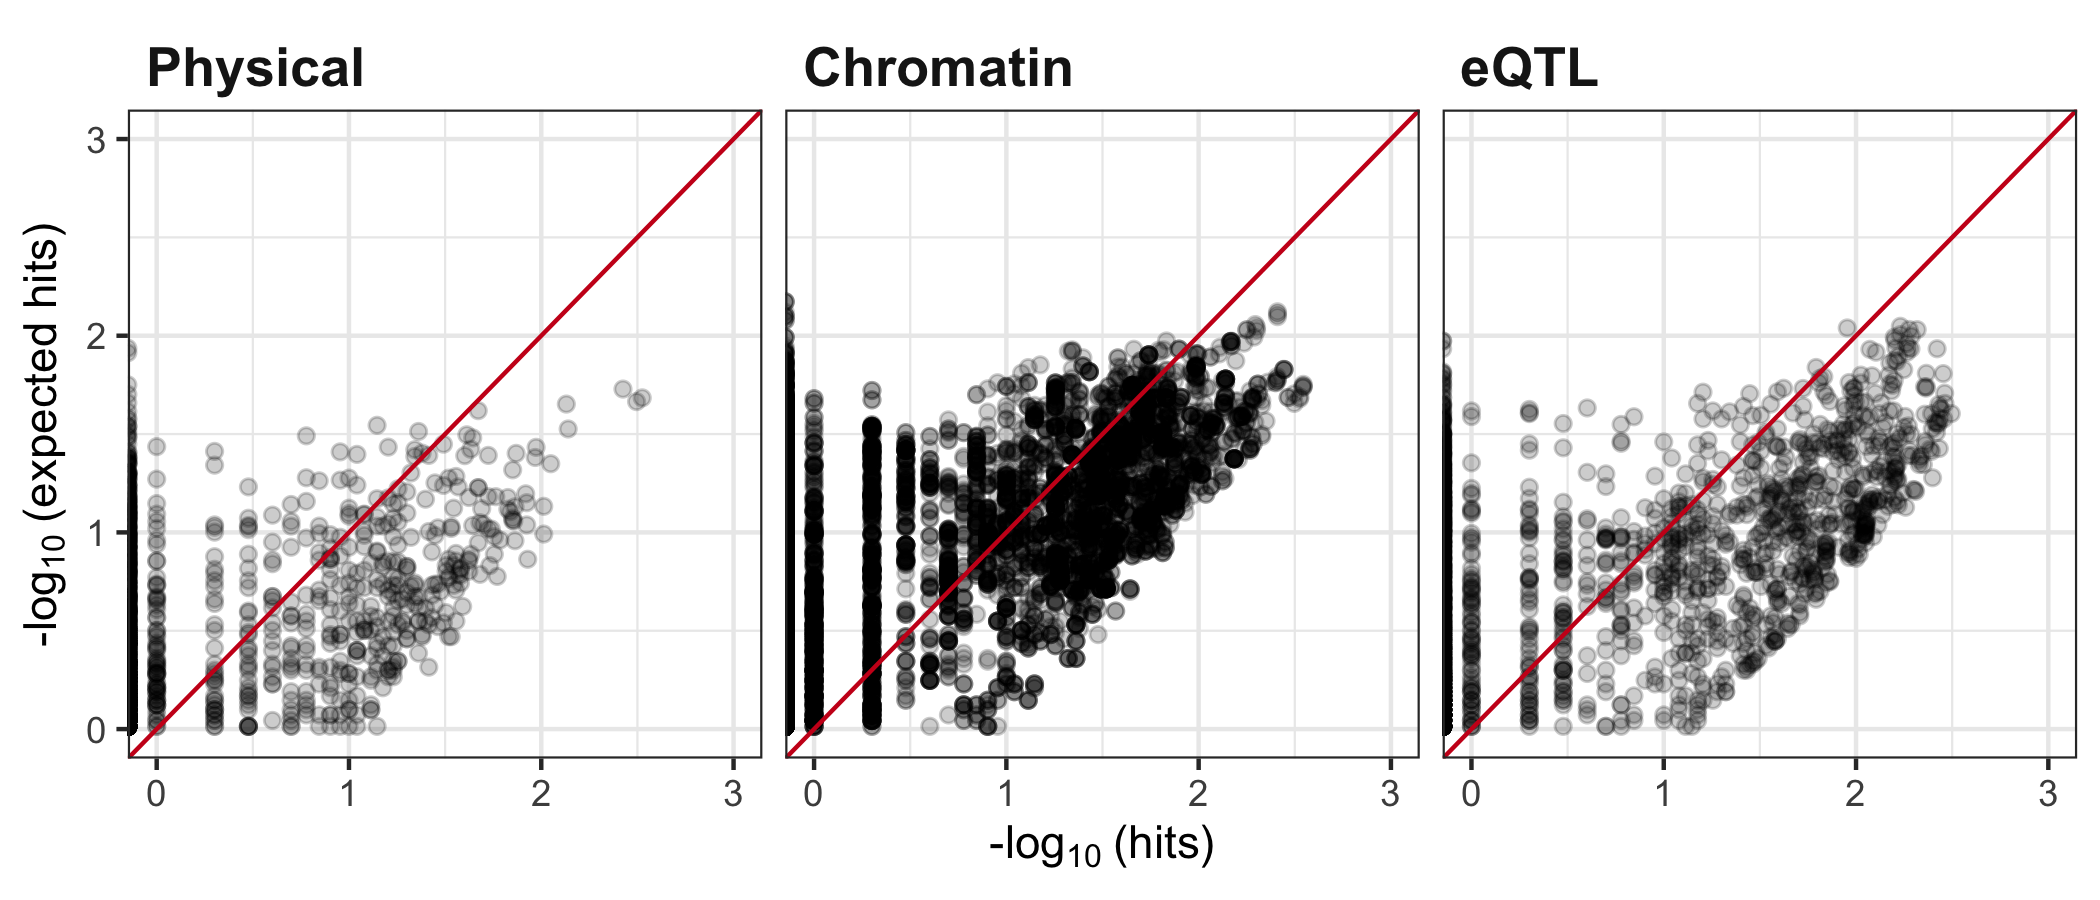
\includegraphics{fig/main_effect_bias.png}
\caption{\label{fig:platform-bias}Plaform bias in the genes hit by SNPs with significant main effects. Every data point is a gene. The \emph{x}-axis represents the number of significant SNPs mapped to that gene. The \emph{y}-axis represents the expected number, if a random set of SNPs of the same size were selected \(\left( \frac {\text{(# significant SNPs)} \times \text{(# SNPs mapped to gene)}} {\text{# SNPS}} \right)\). In red, a line with a slope of 1 representing the case were SNPs are selected at random.}
\end{figure}

Hence, I propose computing the gene
background in a dataset specific way. For instance, the \emph{Chromatin}
results are analyzed in a gene universe where only the genes with a chromatin
mapping to the chip are used. However not all genes are surveyed at the same
resolution, as we observe in Figure \ref{fig:sign-snps-per-gene-and-viceversa}.
If two genes are equally involved in a disease, we are more likely to find an
association in the gene which we are testing more often. Hence, I would like to
weigh every gene by the number of SNPs that map to it, which should provide
a conservative null hypothesis.

Lastly, the protocol presented here is a
complex, multi-stage approach which can be useful to any researcher with any
GWAIS dataset. In consequence, it would be useful to provide a dataset-agnostic
computational pipeline. The user would just need to provide a gene-gene network,
a SNP-gene mapping, and a GWAIS dataset, and would be given two epistasic
networks, SNP- and gene-based respectively. Generating such a pipeline would
also allow us to answer the questions outlined above faster.

\hypertarget{epi-network}{%
\chapter{High-order epistasis detection through fusion of epistasis networks}\label{epi-network}}

The contents of this chapter are based on \emph{Héctor Climente-González, Diane Duroux, Chloé-Agathe Azencott, Kristel Van Steen}, High-order epistasis detection through fusion of epistasis networks (manuscript in preparation).

\begin{chapabstract}{Abstract:}
In this chapter we explore the detection of high-order epistasis in inflammatory bowel disease (IBD). We model high-order epistasis through a linear regression with interaction terms of orders up to 4. The number of tests increases exponentially with the order of the interactions, resulting in low statistical power and computational challenges. To tackle this, we devised a two-step approach to restrict the number of tests. In a first step, we apply a variety of second-order epistasis detection methods, and build an epistasis network that aggregates all the detected interactions. In a second step, we take all star subnetworks composed of 3 and 4 nodes, and search for high-order epistasis between them. The rationale is that SNPs involved in high-order epistasis are more likely to display second-order as well. The advantage of this approach is that we keep the number of tests under control, performing 124 tests instead of the $5 \times 10^{17}$ required to exhaustively search order 4 interactions. Indeed, we are able to detect 37 high-order interactions (FDR 10\%). Mapping these SNP-SNP interactions to gene-gene interactions suggests the involvement of the complement system in susceptibility to IBD.
\end{chapabstract}
\vskip 0.2in
\begin{chapabstract}{Résumé :}
Dans ce chapitre nous nous int\'eressons \`a la d\'etection d'interactions 
\'epistatiques d'ordre sup\'erieur dans les maladies chroniques 
inflammatoires de l'intestin (MICI). Nous mod\'elisions ces interactions 
par une r\'egression lin\'eaire comportant des termes d'interaction allant 
jusqu'\`a l'ordre 4. Le nombre de tests statistiques augmentant de façon 
exponentielle avec l'ordre des interactions, cela r\'eduit fortement la 
puissance statistiques tout en cr\'eant des difficult\'es calculatoires. 
Pour r\'esoudre ces probl\`emes, nous proposons une approche en deux \'etapes 
pour r\'eduire le nombre de tests. Dans la premi\`ere \'etape, nous appliquons 
diverses m\'ethodes de d\'etection d'\'epistasie d'ordre 2, et construisons un 
r\'eseau d'\'epistasie qui agr\`ege toutes les interactions ainsi d\'ecouvertes. 
Dans un second temps, nous testons tous les sous-r\'eseaux en \'etoiles de 3 
ou 4 nœuds. Nous faisons ici l'hypoth\`ese que les SNPs impliqu\'es dans des 
interactions d'ordre 3 ou 4 sont plus susceptibles d'apparaître aussi 
dans des interactions d'ordre 2. L'avantage de notre approche est de 
contr\^oler fortement le nombre de tests statistiques, ici 124 au lieu des 
$5 \times 10^{17}$ requis pour une recherche exhaustive. Cela nous 
permet de d\'etecter 37 interaction d'ordre 3 ou 4 (FDR 10\%). Traduire 
ces interactions SNP-SNP en interactions g\`ene-g\`ene sugg\`ere l'implication 
du syst\`eme du compl\'ement dans la susceptibilit\'e aux MICI.
\end{chapabstract}

\hypertarget{introduction-3}{%
\section{Introduction}\label{introduction-3}}

Although in the previous chapter we focused on interactions between two loci, some studies suggest that high-order epistasis, interactions between more than two loci, that is to say, strongly shapes complex traits (Taylor and Ehrenreich \protect\hyperlink{ref-taylor_higher-order_2015}{2015}). However, exhaustively searching for high-order epistasis aggravates the challenges of GWAIS (Section \ref{gwais}): a large number of statistical tests to consider, higher diversity of ways an interaction can occur, and results harder to interpret. Under the rationale that high-order interactions are likely to show also second-order effects, second-order epistasis networks have been leveraged on in the past to detect high-order epistasis (Hu et al. \protect\hyperlink{ref-hu_statistical_2012}{2012}). In this chapter we explore high-order epistasis interactions in IBD using a similar approach. We do so in two steps. First, we apply a representative variety of second-order epistasis detection methods, and construct an epistasis network. Then we search for high-order epistasis between the SNPs in the network and their neighbors. As in Chapter \ref{genesis}, the first step also allows us to compare the different methods.

\hypertarget{materials-and-methods-1}{%
\section{Materials and methods}\label{materials-and-methods-1}}

\hypertarget{data-quality-control-and-preprocessing}{%
\subsection{Data, quality control and preprocessing}\label{data-quality-control-and-preprocessing}}

We studied genetic data from the IIBDGC (Section \ref{iibdgc-dataset}), and performed a quality control and preprocessing as in Section \ref{snp2gene-qc}. Lastly, we performed LD pruning \(R^{2}>0.75\) to remove SNPs in strong LD, taking down the final number of SNPs to 38,225, which yields \(7.3 \times 10^8\) pairs to test. In this chapter we did not apply any functional pre-filter to the data.

\hypertarget{methods-methods}{%
\subsection{Epistasis detection methods}\label{methods-methods}}

We applied a selection of epistasis detection methods that can process continuous phenotypes and that had a ready-to-use implementation.

\hypertarget{linear-regression}{%
\subsubsection{Linear regression}\label{linear-regression}}

As in Section \ref{methods:snp-epistasis}, we explored two-way epistasis using a linear regression. In this case, we accounted for multiple testing by setting the family-wise error rate to 0.05.

\hypertarget{mb-mdr}{%
\subsubsection{MB-MDR}\label{mb-mdr}}

MB-MDR (Lishout et al. \protect\hyperlink{ref-lishout_efficient_2013}{2013}) is an extension of the classical MDR method (Moore et al. \protect\hyperlink{ref-moore_flexible_2006}{2006}). For a pair of SNPs, MDR classifies every pair of alleles as either high risk, or low risk, depending on whether for the examined combination, the cases/controls ratio is positive or negative, respectively. In a cross-validation setting, the SNP-pairs are ranked using the classification accuracy on unseen samples. MB-MDR includes improvements over the MDR algorithm. First, it accounts for ambiguous pairs of alleles where the number of cases and controls are similar, boosting generalization. Second, MB-MDR extends MDR to continuous phenotypes. This is done by performing a \emph{t}-test that compares the continuous trait between the samples with a specific a pair of alleles with that of the samples with any other combination. If such difference is significant, the combination of alleles is classified as high risk or low risk, depending on the directionality of the change; else, it is considered ambiguous.

We ran MB-MDR with 999 permutations, and a codominant encoding. We kept interactions with a P-value \textless{} 0.05 as in Lishout et al. (\protect\hyperlink{ref-lishout_efficient_2013}{2013}).

\hypertarget{epihsic}{%
\subsubsection{EpiHSIC}\label{epihsic}}

EpiHSIC (T. Kam-Thong et al. \protect\hyperlink{ref-kam-thong_epistasis_2011}{2011}) is a generalization to continuous phenotypes of EPIBLASTER (Tony Kam-Thong et al. \protect\hyperlink{ref-kam-thong_epiblaster-fast_2011}{2011}), which works on case-control studies. EPIBLASTER detects epistasis in a two stage approach. First all SNP pairs are screened using the difference in Pearson's correlation between two SNPs between cases and controls. Then, a logistic regression is used to detect epistasis among the candidate SNP pairs, similar to our what we do in Section \ref{methods:snp-epistasis}. T. Kam-Thong et al. (\protect\hyperlink{ref-kam-thong_epistasis_2011}{2011}) show that the difference in correlation coefficients is an instance of the Hilbert--Schmidt Independence Criterion (HSIC) which a particular choice of kernels. In EpiHSIC they propose a different selection of kernels that extends the screening step to continuous phenotypes. We used \emph{gpuEpiScan}'s R implementation of this algorithm (Jiang \protect\hyperlink{ref-gpuEpiScan}{2019}).

\hypertarget{methods-high-order}{%
\subsection{High-order epistasis detection}\label{methods-high-order}}

We built a SNP-SNP epistasis network using all the significant interactions from the presented methods. On this network, we selected star networks (one central node connected to all the others) as candidate sets for high-order epistasis detection. For each candidate set we built a linear model that included all possible interaction terms. For instance, for a network with three SNPs, \emph{A}, \emph{B} and \emph{C}, we built the following model:

\[Y = \beta_0 + \beta_1 g_A + \beta_2 g_B + \beta_3 g_A g_B + \beta_4 g_A g_C + \beta_5 g_B g_C + \beta_6 g_A g_B g_C,\]

where the coefficients are the \(\beta\) terms, and \(g_A\), \(g_B\) and \(g_C\) are the genotypes under additive encoding for SNPs \emph{A}, \emph{B} and \emph{C} respectively. We consider that there is a 3-way epistatic interaction between these three genes if \(\beta_6\) is significantly different from 0. As under the null hypothesis the \(\beta\) coefficients follow a standard Normal distribution, we evaluated a departure from it using a \emph{t}-test. We restricted the sets to star subnetworks of size 3 and 4, as the number of tests grows exponentially with the number of SNPs. We accounted for multiple testing by setting the false discovery rate to 10\%. For this purpose, the total number of tests was the number of \(\beta\) for terms of order 3 and 4 for which a \(\beta\) was obtained.

\hypertarget{code-availability}{%
\subsection{Code availability}\label{code-availability}}

The different epistasis detection methods are implemented in pipelines with a similar interface, available on GitHub (\url{https://github.com/hclimente/gwas-tools}). The code necessary to reproduce this chapter's results, altogether with the corresponding analyses, are available on GitHub as well (\url{https://github.com/hclimente/waffles}).

\hypertarget{results-1}{%
\section{Results}\label{results-1}}

\hypertarget{epistasis-detection-methods-produce-relatively-similar-results}{%
\subsection{Epistasis detection methods produce relatively similar results}\label{epistasis-detection-methods-produce-relatively-similar-results}}

We applied different methods to search for epistatic interactions in the IIBDGC dataset (Section \ref{methods-methods}). From these interactions, we built an epistasis network that included all significant pairs from any of the methods. In total they retrieved 823 epistatic interactions involving 459 SNPs (Figure \ref{fig:overview}). MB-MDR is the method that detects the largest number of interactions (741), followed by logistic regression (68) and EpiHSIC (14). This is not surprising, since we did not apply any multiple testing correction to MB-MDR's output. Despite difference in size, MB-MDR's solutions greatly overlap with logistic regression's (37, 54.4\%) and EpiHSIC (3, 21.4\%) (Figure \ref{fig:solutions-overlap}). In the same vein, 110 of the 459 SNPs in epistasis have significant main effects themselves (Fisher's Exact Test \(\text{P-value} < 2.2 \times 10^{-16}\) on the overlap), despite both MB-MDR and logistic regression accounting for main effects. This large overlap points to a large agreement on the biological mechanisms of the disease. It also motivates searching for high-order epistasis preferentially among the subset of SNPs involved in second order interactions.



\begin{figure}
\centering
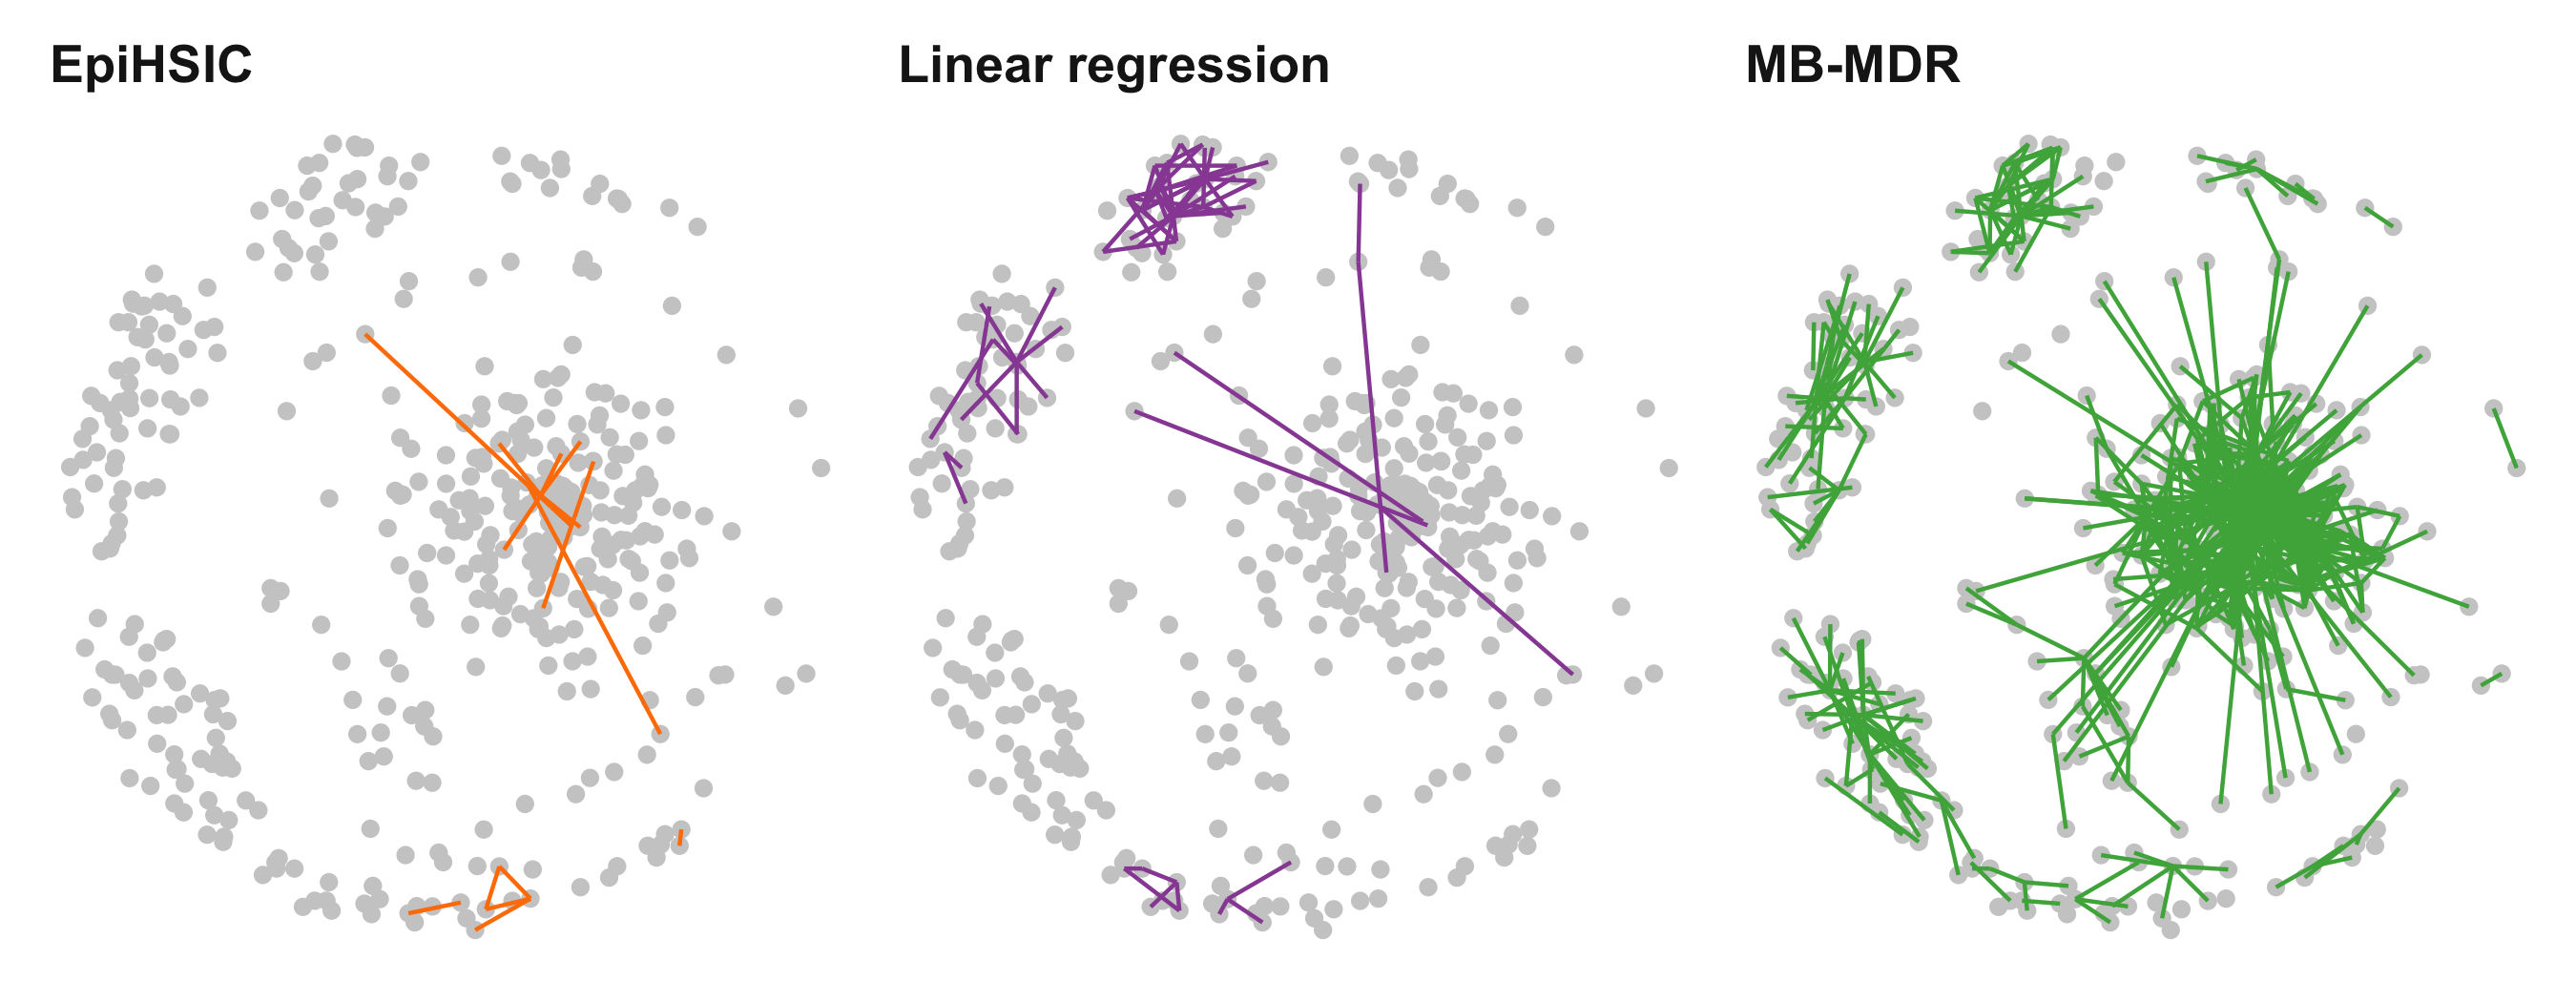
\includegraphics{fig/overview_snp_solutions.png}
\caption{\label{fig:overview}Overview of the SNP epistasis networks produced by different epistasis detection (Section \ref{methods-methods}). The network is split into several panels to depict the source of each interaction.}
\end{figure}



\begin{figure}

{\centering 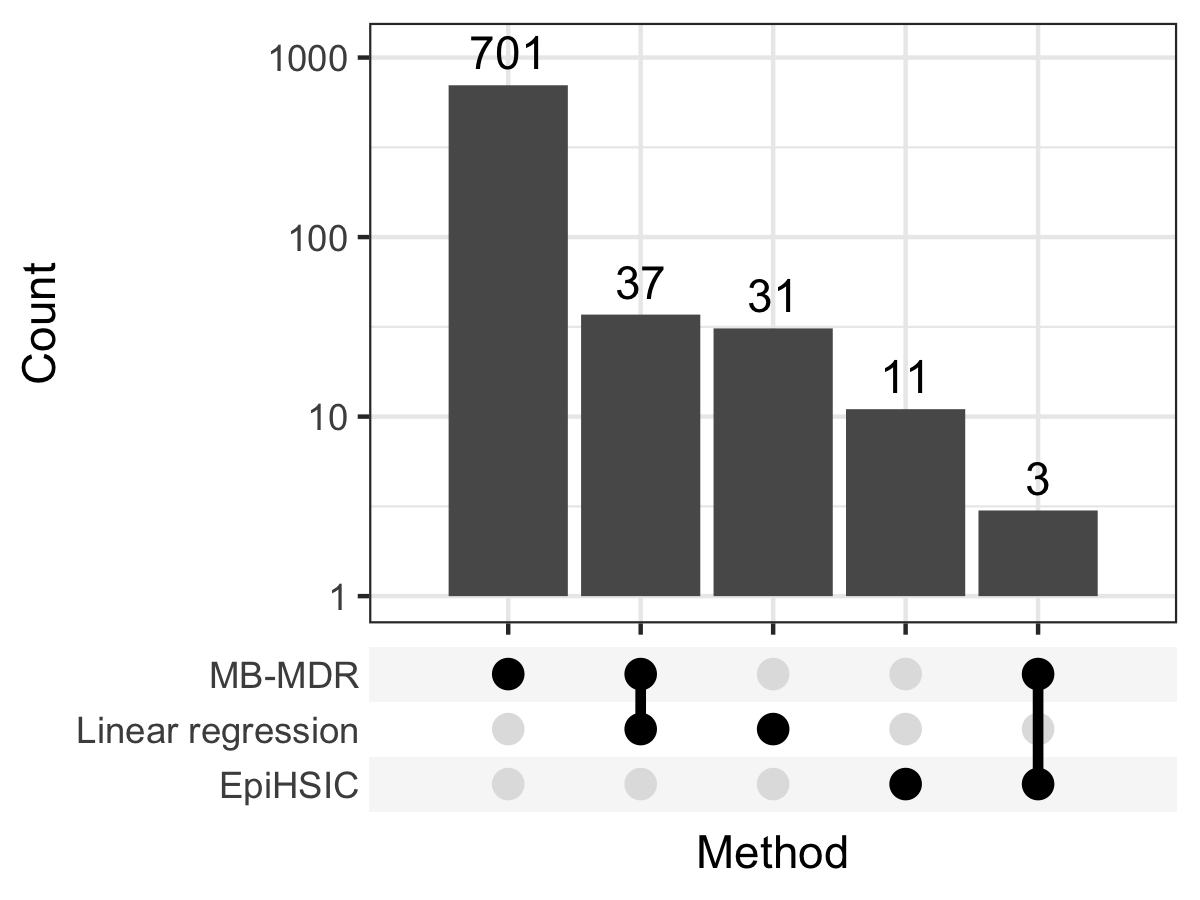
\includegraphics[width=0.6\linewidth]{fig/overlap_solutions} 

}

\caption{Overlap between the solutions from the different epistasis detection methods. Note that the \emph{y}-axis is in logarithmic scale.}\label{fig:solutions-overlap}
\end{figure}



\begin{figure}
\centering
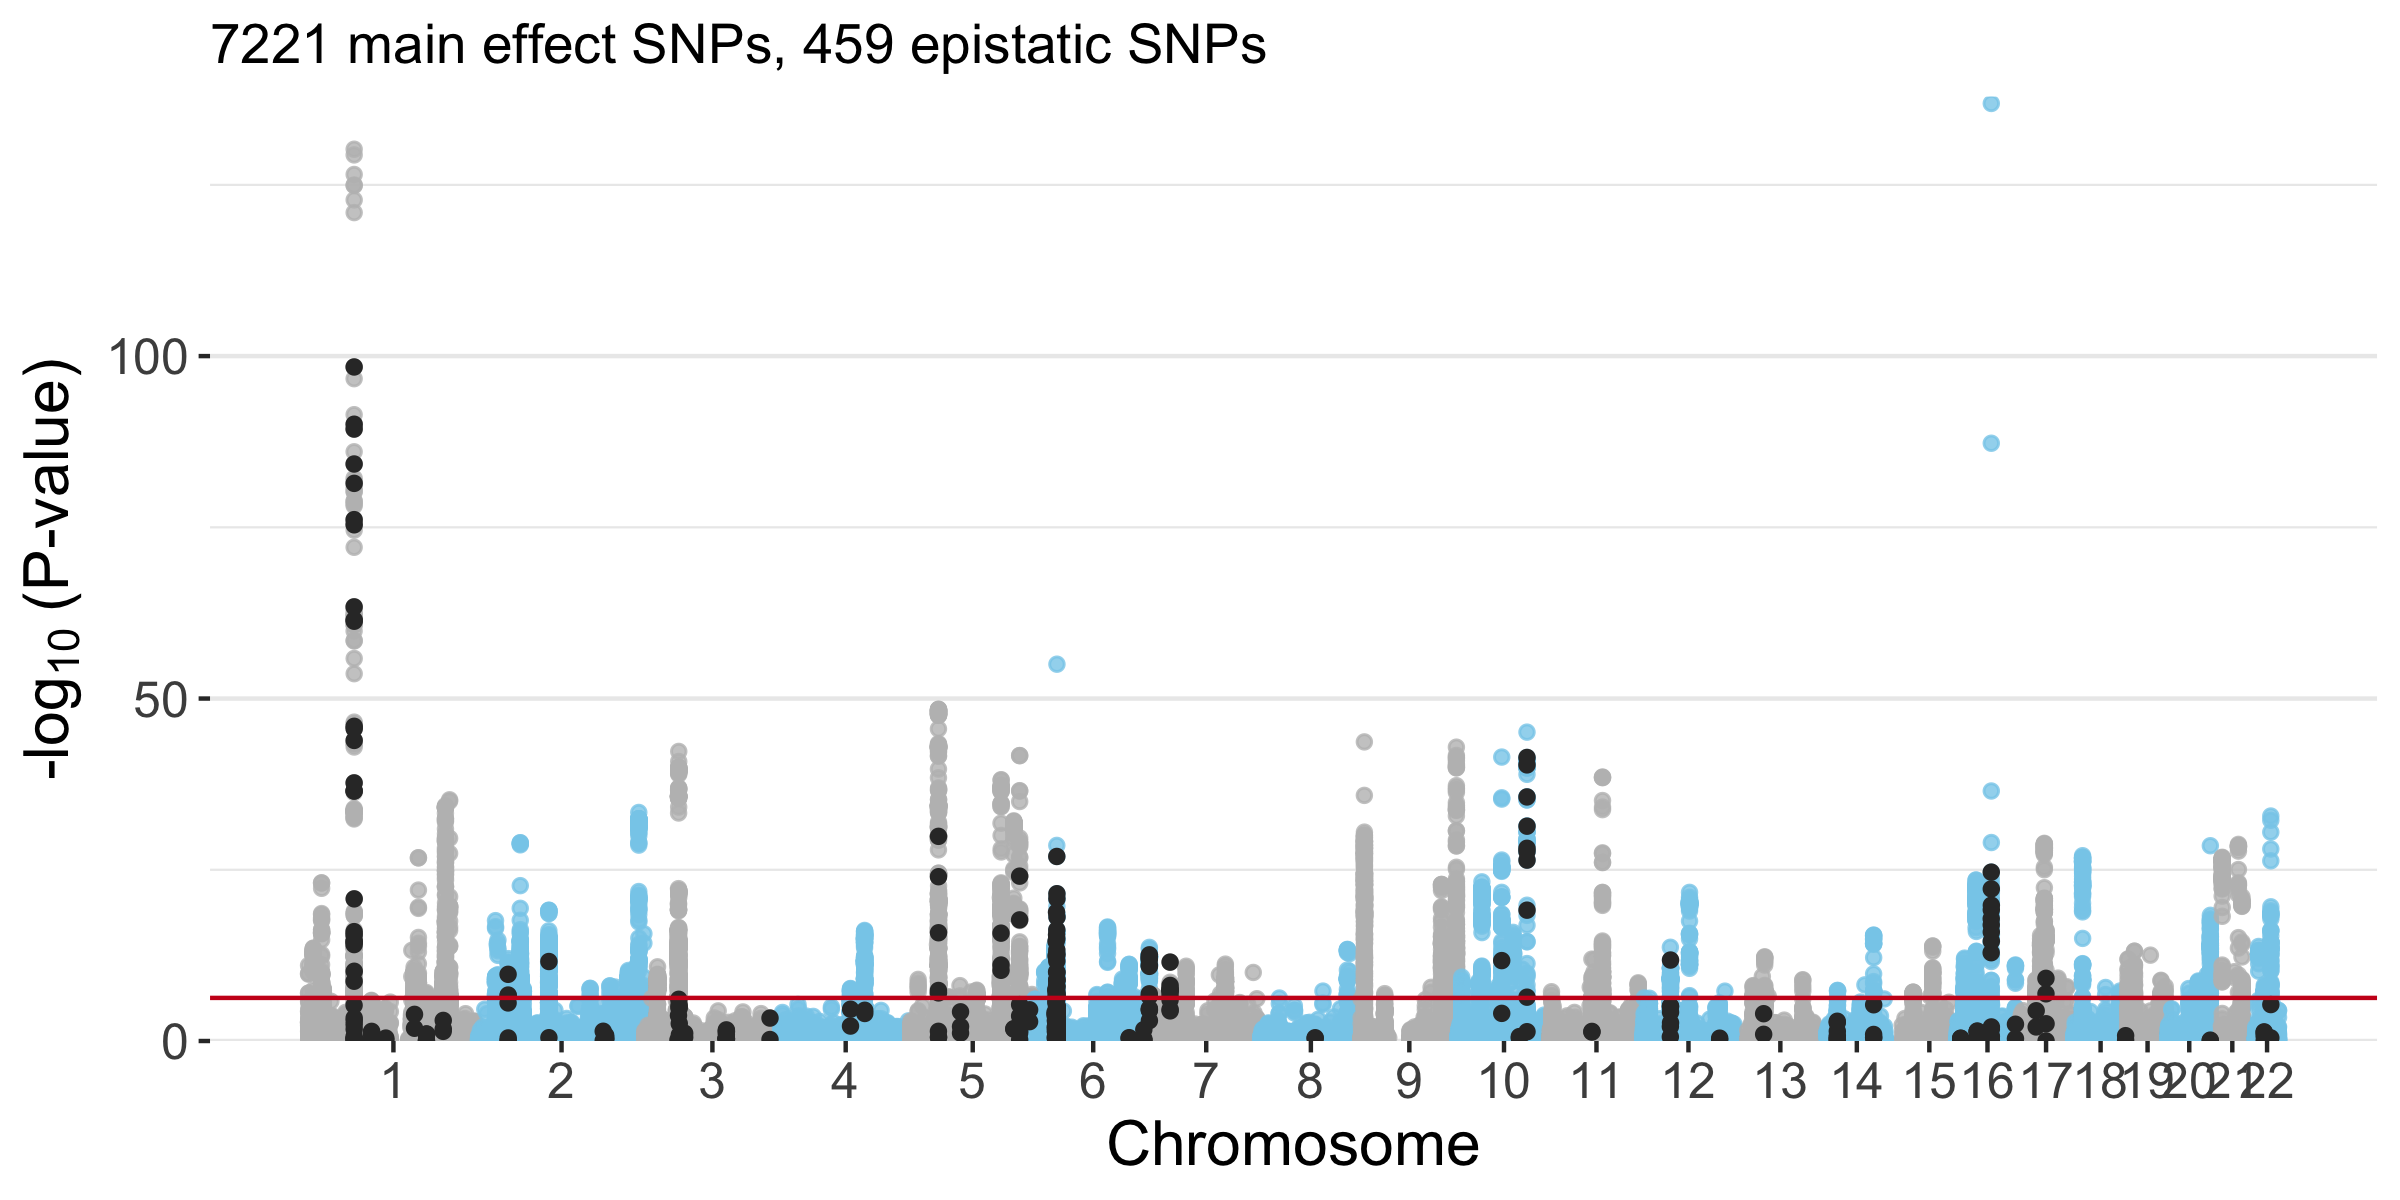
\includegraphics{fig/manhattan_epistasis.png}
\caption{\label{fig:main-effect-overlap}Main effects on IBD, measured using a logistic regression on the case-control phenotype. The 7 largest principal components are included in the model as covariates. SNPs involved in an epistasis interaction are colored in dark grey.}
\end{figure}

\hypertarget{high-order-epistasis-interactions-in-ibd}{%
\subsection{High-order epistasis interactions in IBD}\label{high-order-epistasis-interactions-in-ibd}}

We searched for 3rd and 4th order epistasis in 124 star subnetworks from the aggregated network (Section \ref{methods-high-order}). Out of them 37 are significant at FDR 10\% (Figure \ref{fig:high-order}). The high proportion of the tested interactions that are significant (29.8\%) supports the pertinence of our approach. Only three of the tested star subnetworks involved edges from different sources, probably due to the difference in solution size between MB-MDR and the other methods.



\begin{figure}

{\centering 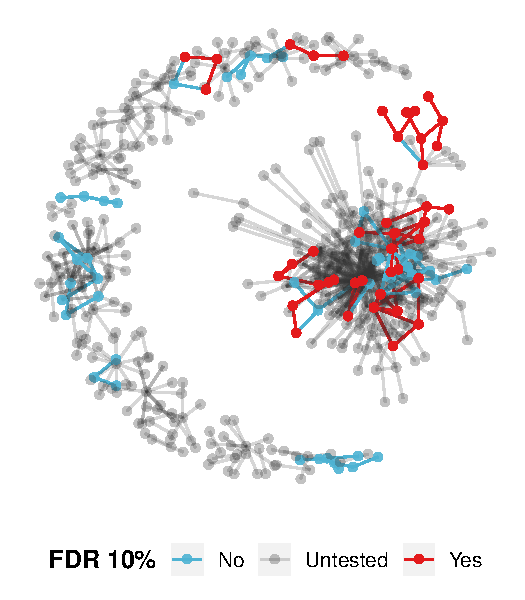
\includegraphics[width=0.6\linewidth]{fig/high_order_significant} 

}

\caption{Overview of the detected high-order epistasis interactions, shown on the binary epistasis network. The edges involved in the 124 tested 3rd and 4th order interactions are highlighted in blue; the 37 among those that were significant, in red.}\label{fig:high-order}
\end{figure}

\hypertarget{mapping-snp-to-genes-involves-the-complement-system}{%
\subsection{Mapping SNP to genes involves the complement system}\label{mapping-snp-to-genes-involves-the-complement-system}}

We mapped the 823 SNP-SNP interactions to gene-gene interactions. We used any of the maps described in Section \ref{methods:prefiltering}, using exclusively genes with a HUGO symbol. As in Chapter \ref{epi-snp2gene}, we removed genes in the HLA regions and self-interactions. But, in contrast with that chapter, we make use of all three mappings at once, and hence expect gene-gene interactions where the genes were mapped via two different mappings. This resulted in 1,113 different genes and 20,826 different gene-gene interactions. When we restricted ourselves only to those binary interactions involved in one of the 37 significant high-order interactions, we obtained 162 genes and 5,273 candidate gene-pairs. This one-to-many mapping illustrates well the problem of linking SNP-SNP interactions to their functional consequences. Restricting the 5,273 interactions only to those that exist on STRING (Szklarczyk et al. \protect\hyperlink{ref-szklarczyk_string_2019}{2019}), we reduced the number to 892 interactions involving 94 genes. We decided to focus on this latter set of interactions. Although it is doubtful that all these gene-gene interactions are truly linked to the disease, we conjecture that it will be enriched in relationships truly associated to the disease. The high interconnectedness of the network (Figure \ref{fig:overview}) gives support to this idea, seeming to capture a reduced number of susceptibility mechanisms.

We first studied how many SNP-SNP interactions supported every gene-gene interaction. The gene-gene interactions with higher support involve immunity-related genes. More specifically, they involve multiple genes from the complement system (\emph{C4A}, \emph{C4B} and, to a lesser extent, \emph{C2}). This set of genes is part of the innate system, and is part of the organism's reaction to pathogens. The involvement of the complement system in IBD has received some attention lately (Jain et al. \protect\hyperlink{ref-jain_complement_2014}{2014}; Heybeli \protect\hyperlink{ref-heybeli_complement_2016}{2016}; Sina, Kemper, and Derer \protect\hyperlink{ref-sina_intestinal_2018}{2018}), as mice lacking complement proteins suffer intestinal infammation similar to IBD. In our results, we observe an interaction between the three aforementioned genes of the complement, and in greater numbers with other genes, the one supported by most SNP-SNP interactions being \emph{NOTCH4}.

\hypertarget{discussion-1}{%
\section{Discussion}\label{discussion-1}}

In this chapter I apply three methods for second order epistasis detection to the IIBDGC dataset. Most of the detected interactions came from the same method, MB-MDR, which exhibited a high sensitivity. Consistent with the observation that SNPs with main effects are involved in such epistatic interactions, we detected 3rd and 4th order interactions between the many SNPs with two-way epistasis. When we mapped the SNP pairs to candidate gene pairs, we observed that many gene-gene interactions involved genes involved in the complement system. This gives a genetic rationale to the recent observations of the involvement of the complement system in the etiology of IBD.

However, our approach has some shortcomings. First, searching for high-order epistasis in hubs from the epistatis network is not possible under the current approach. For instance, the node with the highest degree has 39 neighbors, which implies building a model which includes interaction terms up to order 39. In this regard, a possible way forward would be dividing such star subnetworks into sets of 3 and 4 nodes, and looking exclusively for 3rd and 4th order interactions respectively within them. Another issue is the mapping of SNPs pairs to gene pairs. In this regard, our work in Chapter \ref{epi-snp2gene} is promising, and answering the questions remaining in that project will pave the way to this one. Some of these questions are whether it is beneficial to use tissue-specific SNP-gene mappings, when should a gene-gene filter be used, or how to appropriately carry out a pathway enrichment analysis on epistasis results. However, this chapter presents new challenges in these fronts as well, like how to use binary interactions when we work on ternary interactions. Although here I decomposed them into binary interactions, it is worth considering higher order gene-interactions obtained from databases, namely co-complexes. Another open question is how the results of the presented approach compare to the results of existing methods to detect high-order interactions (Llinares-López et al. \protect\hyperlink{ref-llinares-lopez_casmap_2018}{2018}; Suzumura et al., \protect\hyperlink{ref-suzumura_selective_nodate}{n.d.}; Terada et al. \protect\hyperlink{ref-terada_lamplink_2016}{2016}).

Additionally, in this study we faced a scarcity of methods that work on continuous phenotypes or accept covariates. Such methods are necessary to account for population structure in epistasis detection. In this chapter I have presented three such methods, and we have located a few more: GenEpi (Chang et al. \protect\hyperlink{ref-chang_genepi:_2018}{2018}), and several approaches based on random forest-based approaches (Yoshida and Koike \protect\hyperlink{ref-yoshida_snpinterforest:_2011}{2011}; Li et al. \protect\hyperlink{ref-li_detecting_2016}{2016}) or mutual information (Pensar et al. \protect\hyperlink{ref-pensar_genome-wide_2019}{2019}). Adding some of these methods to protocol is likely to increase the number of detected high-order interactions. Additionally, I see this as a good opportunity to compare the methods, as has been done already on methods that work on case-control phenotypes (Shang et al. \protect\hyperlink{ref-Shang2011}{2011}; Chatelain et al. \protect\hyperlink{ref-chatelain_performance_2018}{2018}).

\hypertarget{conclusions-1}{%
\chapter{Conclusions}\label{conclusions-1}}

In the last 10 years great progress has been made in the understanding of the genetic architecture of complex diseases through GWA(I)S. That success would not have been possible without the effort of multiple national and international consortia who coordinated research groups to tackle specific diseases. Nonetheless, the GWA(I)S experimental settings present challenges that hinder the discovery of susceptibility mechanisms, our understanding of biology and, ultimately, improving diagnosis and clinical care. Some of these challenges are low statistical power, the difficulty to link associated genotypes to functional changes, the multiplicity of ways to detect epistasis, and properly accounting for LD in the statistical treatment of the data. During my PhD I have explored how network methods can be used to tackle these challenges.

In \textbf{Chapter \ref{genesis}} we applied and critically evaluated different high-score subnetwork search methods to the GENESIS breast cancer GWAS dataset. Such methods are particularly relevant in GWAS, as they address some of the drawbacks of the experimental setting: low statistical power and interpretability. Most network methods produced a biologically plausible answer, which by itself deepens our understanding of the susceptibility mechanisms acting out in this specific trait. However, this methodological comparison also highlights how radically different the solutions are from each other. This is the product of different ways of modeling the informal concept of high-score subnetwork mathematically. We combined the different solutions into a consensus network, which was simpler than the largest individual solutions, but preserved their most important topological and biological properties. Network aggregation is a promising approach to the multiplicity of network methods.

In \textbf{Chapter \ref{martini}} I presented \emph{martini}, an R implementation of SConES, one of the methods I used in \textbf{Chapter \ref{genesis}}, that addresses some of its initial shortcomings, extending it to case-control phenotypes, and adding hyperparameter selection options and support for covariates. As I show Chapter \ref{genesis}, and expand in this chapter, SConES is a particularly flexible algorithm among high-score subnetwork search methods. Specifically, it has two hyperparameters that allow to fine-tune the topology and the sparsity of the selected subnetwork. Unfortunately, this flexibility comes at the price of appropriately tuning these parameters, an issue that is exacerbated by the instability of the solutions. In this regard, the feature selection scores I implemented helped finding more realistic solutions in some simulations, although one could still improve upon this proposition. One possibility would be to score the solution using the topology (edge density, centrality betweenness, number of connected components).

In \textbf{Chapter \ref{epi-snp2gene}} we propose a protocol to improve both the statistical power and the interpretability of GWAIS, and apply it to the IIBDGC dataset. In essence, we employ three different ways of mapping SNPs to known gene interactions (physical, eQTL, and chromatin), and only test the corresponding pairs of SNPs. Indeed, we observe that the proposed protocols reduce the number of tests, and detect interpretable interactions which are not found using a conventional approach. For instance, the eQTL filter produces more SNP interactions than any other mapping, while the chromatin filter detected gene interactions that are strongly related to interleukins, a immune system family of molecules involved in IBD. Despite the promising results, there are two aspects of the protocol that need to be refined: decoupling SNP-gene mapping from known gene interactions, to study the contribution of each to the positive results; and topping the protocol with an approach to map the detected interactions to affected pathways.

In \textbf{Chapter \ref{epi-network}} I apply a strategy for high-order epistasis detection to IBD. In essence, it consists of two steps. The first step involves building a SNP-SNP epistasis network using multiple epistasis detection tools. The second one consists on searching high-order epistasis between specific nodes of the network and their neighbors. Indeed, this approach boosts the statistical power of high-order epistasis detection by reducing the number of tests by 15 orders of magnitude, and allows us to detect 37 high-order interactions. In an exercise similar in its spirit to that of Chapter \ref{epi-snp2gene}, we map these interactions to known gene-gene interactions using functional SNP-gene mappings. In this way we link the detected interactions to the complement system, an emergent candidate susceptibility mechanism to IBD.

In this thesis I illustrated several hurdles in our way to identifying and understanding the genetics of complex diseases. I now conclude with a look into the state of the field, and future research directions related to my contribution.

\textbf{The future of network methods for GWAS.} The network methods I worked with during my PhD are notably heterogeneous. Although that heterogeneity stems from divergences in what different researchers aim to find, being able to obtain different points of view from a disease is a strength. However, clearer language and more exhaustive comparisons to other methods would be well-received in the methods' publications. With the exception of SConES, all high-score subnetwork search methods I tested work on gene-gene interaction networks. SConES on the other hand uses SNP-SNP networks. The latter kind of networks operate at a lower level than the gene and, hence, potentially can handle more information. For instance, it could contain information about the specific protein residues that participate in a protein-protein interface. It could also encode LD blocks, by weighing the edges of the network proportionally to the correlation between SNPs. The benefits from using SNP-SNP networks are highlighted by the the biologically relevant results obtained with SConES even when no protein-protein information was added to the SNP network. On the other hand, the SNP networks that I handled in this thesis were orders of magnitude more complex than the corresponding protein-protein interaction networks for the same dataset. This increases runtime prohibitively, and new methods, or faster versions of the current ones, are required to explore the potential of such, more informative, SNP networks.

\textbf{The role of network methods in bioinformatics.} My experience with network methods sometimes clashed with other people's impressions of the field during informal exchanges. In particular, some researchers receive network results and methods with a mix of puzzlement in the face of the overwhelming amount of information they represent, and a subsequent skepticism. In my opinion, this anecdotal evidence speaks to the state of network biology as a field, which lacks clear, agreed on, protocols and goals. Hence, I believe a multi-front effort must be made to close this gap. A first line of attack involves more accessible tools, with similar interfaces and proper documentation. One of my goals in Chapter \ref{genesis} was to create such an interface for the tools I used. Another subject to tackle is the development of better tools to visualize and manipulate network results. Innovative visualizations like hive plots (Krzywinski et al. \protect\hyperlink{ref-krzywinski_hive_2012}{2012}), and the package \emph{tidygraph} to manipulate networks (Pedersen \protect\hyperlink{ref-pedersen_tidygraph_2019}{2019}) are moves in the right direction. Interaction databases are also part of the inaccessibility issue: Huang et al. (\protect\hyperlink{ref-huang_systematic_2018}{2018}) evaluated 21 such databases, often collecting overlapping information, and with unclear definitions of what \emph{interaction} means. Efforts must be unified towards a single database, with a user-friendly interface and clarity about its contents -- with the caveat that such efforts may simply result in yet another database that will be used in parallel with the others\footnote{\url{https://xkcd.com/927/}}. In this regard, I believe HINT (Das and Yu \protect\hyperlink{ref-das_hint_2012}{2012}), which aggregates multiple databases, is a step in the right direction. This relates to the issue, also discussed in Chapter \ref{genesis}, of the different types of biological interactions: despite the preponderance of protein-protein interactions, other types of interactions (like RNA -- RNA or transcription factor -- DNA) need to be better compiled and characterized.

\textbf{The future of GWAS.} Despite the issues I discussed, GWAS have had a sound success in identifying genetic associations with complex traits, therefore helping understanding their genetic basis. Many past and present initiatives are leveraging on more data to solve some of these issues: massive prospective cohort studies like UK Biobank (Sudlow et al. \protect\hyperlink{ref-sudlow_uk_2015}{2015}), more GWAS on understudied populations, and initiatives in functional genomics like ENCODE (The ENCODE Project Consortium \protect\hyperlink{ref-the_encode_project_consortium_integrated_2012}{2012}). However, many statistical questions remain to be solved. Despite some efforts to unify practices (Wang, Cordell, and Van Steen \protect\hyperlink{ref-wang_statistical_2018}{2018}), the field is dominated by laboratory- and method-specific practices, which are rarely justified in published articles. For instance, whether to LD prune or not; map SNPs to the exact coordinates of a gene, or include some kilobases upstream and downstream; or what is the minimum MAF of SNPs to analyze. An open conversation is needed which confronts different protocols, and reaches consensuses where possible, and justified guidelines when it is not. On this front, network methods can be powerful allies, as shown in Chapter \ref{genesis}, but work in other fields, both experimental and \emph{in silico}, is also required. For instance a proper incorporation of LD patterns to processing analysis might lead to both an increase in statistical power (by reducing the number of tests to one per independent test) and interpretability (by considering the true unit of variation), while accounting for population structure by default (as it is caused by LD). Also, the technology of choice for GWAS is slowly shifting from SNP arrays to the increasingly affordable whole genome-sequencing. This in itself is bringing a substantial change to the GWAS scene, by providing a deeper coverage which includes more rare variants. Nonetheless, this increase in the number of variants studied only increases our need for appropriately treating LD.

\textbf{The future of GWAIS.} Epistasis detection is an open and promising field. As in high-score subnetwork search, and as I describe in Chapter \ref{epi-network}, epistasis detection can be achieved through a multiplicity of tools that model it in different ways. As with the aforementioned network methods, we can exploit that multiplicity by collapsing the results into a unified view of disease. Yet, a few challenges remain ahead. The first one, developed above, is the lack of general guidelines for GWA(I)S. The second one, is the inability of most methods to account for population structure, either by accepting covariates, or by accepting an adjusted, continuous phenotype. This last problem also comes up in the study of continuous phenotypes, which were beyond the scope of this thesis. In Chapter \ref{epi-snp2gene} I explored the possible contribution of functional pre-filtering to epistasis detection. In this regard, and encouraged by my experiences described in Chapters \ref{genesis} and \ref{martini}, I believe in the potential of epistasis-detection methods that exploit prior knowledge in the form of a network.

\textbf{Open science with sensitive data.} I would like to finish reflecting about my experience on \emph{open science} as a GWAS researcher. Understandably, GWAS data from human samples requires a careful treatment, as it contains very sensitive information about both the participants and their families. For that reason, working on GWAS data requires compromising on open data, one of the pillars of open science. Hence, at the moment, work on genetic data requires trust from all the other researchers who do not have access to a particular dataset. This might change in the future, when data obfuscation solutions that allow to operate on a dataset while hiding the identifiable information (Azencott \protect\hyperlink{ref-azencott_machine_2018}{2018}) are fully developed. Yet, for the moment, the lack of open data should lead to a stronger commitment to open algorithms and results, to facilitate as much as possible the application of published tools to other datasets and study if the conclusions hold.

\hypertarget{funding-acknowledgments}{%
\chapter*{Funding acknowledgments}\label{funding-acknowledgments}}
\addcontentsline{toc}{chapter}{Funding acknowledgments}

This thesis was funded by the European Union's Horizon 2020 research and innovation program under the Marie Skłodowska-Curie {[}666003{]}. Additionally, the work presented in Appendix \ref{block-hsic-lasso} was made possible by a scholarship from RIKEN AIP, which allowed me to spend 3 months in Makoto Yamada's laboratory in Kyoto.

The co-authors of some chapters, and more generally the work presented in them, received additional sources of funding. Regarding Chapter \ref{genesis}, it was supported by funding from Agence Nationale de la Recherche (ANR-18-CE45-0021-01). Financial support for GENESIS resource and genotyping was provided by the Ligue Nationale contre le Cancer (grants PRE05/DSL, PRE07/DSL, PRE11/NA), the French National Institute of Cancer (INCa grant No b2008-029/LL-LC) and the comprehensive cancer center SiRIC, (Site de Recherche Intégrée sur le Cancer: Grant INCa-DGOS-4654). Computational resources for Chapters \ref{epi-snp2gene} and \ref{epi-network} have been provided by the Consortium des Équipements de Calcul Intensif (CÉCI), funded by the Fonds de la Recherche Scientifique de Belgique (F.R.S.-FNRS) under Grant No.~2.5020.11 and by the Walloon Region.

\hypertarget{references}{%
\chapter*{References}\label{references}}
\addcontentsline{toc}{chapter}{References}

\hypertarget{refs}{}
\begin{cslreferences}
\leavevmode\hypertarget{ref-search_newly_2009}{}%
Ahmed, Shahana, Gilles Thomas, Maya Ghoussaini, Catherine S Healey, Manjeet K Humphreys, Radka Platte, Jonathan Morrison, et al. 2009. ``Newly Discovered Breast Cancer Susceptibility Loci on 3p24 and 17q23.2.'' \emph{Nature Genetics} 41 (5): 585--90. \url{https://doi.org/10.1038/ng.354}.

\leavevmode\hypertarget{ref-azencott_machine_2018}{}%
Azencott, C.-A. 2018. ``Machine Learning and Genomics: Precision Medicine Versus Patient Privacy.'' \emph{Philosophical Transactions of the Royal Society A: Mathematical, Physical and Engineering Sciences} 376 (2128): 20170350. \url{https://doi.org/10.1098/rsta.2017.0350}.

\leavevmode\hypertarget{ref-azencott_network-guided_2016}{}%
Azencott, Chloé-Agathe. 2016. ``Network-Guided Biomarker Discovery.'' In \emph{Machine Learning for Health Informatics}, 9605:319--36. Cham: Springer International Publishing. \url{https://doi.org/10.1007/978-3-319-50478-0_16}.

\leavevmode\hypertarget{ref-azencott_efficient_2013}{}%
Azencott, Chloé-Agathe, Dominik Grimm, Mahito Sugiyama, Yoshinobu Kawahara, and Karsten M. Borgwardt. 2013. ``Efficient Network-Guided Multi-Locus Association Mapping with Graph Cuts.'' \emph{Bioinformatics} 29 (13): i171--i179. \url{https://doi.org/10.1093/bioinformatics/btt238}.

\leavevmode\hypertarget{ref-barabasi_network_2011}{}%
Barabási, Albert-László, Natali Gulbahce, and Joseph Loscalzo. 2011. ``Network Medicine: A Network-Based Approach to Human Disease.'' \emph{Nature Reviews Genetics} 12 (1): 56--68. \url{https://doi.org/10.1038/nrg2918}.

\leavevmode\hypertarget{ref-barton_infinitesimal_2017}{}%
Barton, N. H., A. M. Etheridge, and A. Véber. 2017. ``The Infinitesimal Model: Definition, Derivation, and Implications.'' \emph{Theoretical Population Biology} 118 (December): 50--73. \url{https://doi.org/10.1016/j.tpb.2017.06.001}.

\leavevmode\hypertarget{ref-beisser_bionet:_2010}{}%
Beisser, D., G. W. Klau, T. Dandekar, T. Muller, and M. T. Dittrich. 2010. ``BioNet: An R-Package for the Functional Analysis of Biological Networks.'' \emph{Bioinformatics} 26 (8): 1129--30. \url{https://doi.org/10.1093/bioinformatics/btq089}.

\leavevmode\hypertarget{ref-boyle_expanded_2017}{}%
Boyle, Evan A., Yang I. Li, and Jonathan K. Pritchard. 2017. ``An Expanded View of Complex Traits: From Polygenic to Omnigenic.'' \emph{Cell} 169 (7): 1177--86. \url{https://doi.org/10.1016/j.cell.2017.05.038}.

\leavevmode\hypertarget{ref-breyer_expressed_2014}{}%
Breyer, Joan P., Daniel C. Dorset, Travis A. Clark, Kevin M. Bradley, Tiina A. Wahlfors, Kate M. McReynolds, William H. Maynard, et al. 2014. ``An Expressed Retrogene of the Master Embryonic Stem Cell Gene POU5F1 Is Associated with Prostate Cancer Susceptibility.'' \emph{The American Journal of Human Genetics} 94 (3): 395--404. \url{https://doi.org/10.1016/j.ajhg.2014.01.019}.

\leavevmode\hypertarget{ref-brisbin_meta-analysis_2011}{}%
Brisbin, Abra G, Yan W Asmann, Honglin Song, Ya-Yu Tsai, Jeremiah A Aakre, Ping Yang, Robert B Jenkins, et al. 2011. ``Meta-Analysis of 8q24 for Seven Cancers Reveals a Locus Between NOV and ENPP2 Associated with Cancer Development.'' \emph{BMC Medical Genetics} 12 (1): 156. \url{https://doi.org/10.1186/1471-2350-12-156}.

\leavevmode\hypertarget{ref-buniello_nhgri-ebi_2019}{}%
Buniello, Annalisa, Jacqueline A L MacArthur, Maria Cerezo, Laura W Harris, James Hayhurst, Cinzia Malangone, Aoife McMahon, et al. 2019. ``The NHGRI-EBI GWAS Catalog of Published Genome-Wide Association Studies, Targeted Arrays and Summary Statistics 2019.'' \emph{Nucleic Acids Research} 47 (D1): D1005--D1012. \url{https://doi.org/10.1093/nar/gky1120}.

\leavevmode\hypertarget{ref-bush_chapter_2012}{}%
Bush, William S., and Jason H. Moore. 2012. ``Chapter 11: Genome-Wide Association Studies.'' Edited by Fran Lewitter and Maricel Kann. \emph{PLoS Computational Biology} 8 (12): e1002822. \url{https://doi.org/10.1371/journal.pcbi.1002822}.

\leavevmode\hypertarget{ref-button_power_2013}{}%
Button, Katherine S., John P. A. Ioannidis, Claire Mokrysz, Brian A. Nosek, Jonathan Flint, Emma S. J. Robinson, and Marcus R. Munafò. 2013. ``Power Failure: Why Small Sample Size Undermines the Reliability of Neuroscience.'' \emph{Nature Reviews Neuroscience} 14 (5): 365--76. \url{https://doi.org/10.1038/nrn3475}.

\leavevmode\hypertarget{ref-cai_broker_2010}{}%
Cai, James J., Elhanan Borenstein, and Dmitri A. Petrov. 2010. ``Broker Genes in Human Disease.'' \emph{Genome Biology and Evolution} 2 (January): 815--25. \url{https://doi.org/10.1093/gbe/evq064}.

\leavevmode\hypertarget{ref-calderwood_heat_2016}{}%
Calderwood, Stuart K., and Jianlin Gong. 2016. ``Heat Shock Proteins Promote Cancer: It's a Protection Racket.'' \emph{Trends in Biochemical Sciences} 41 (4): 311--23. \url{https://doi.org/10.1016/j.tibs.2016.01.003}.

\leavevmode\hypertarget{ref-Chaiboonchoe2013}{}%
Chaiboonchoe, Amphun, Wiktor Jurkowski, Johann Pellet, Enrico Glaab, Alexey Kolodkin, Antonio Raussel, Antony Le Béchec, et al. 2013. ``On Different Aspects of Network Analysis in Systems Biology.'' In \emph{Systems Biology: Integrative Biology and Simulation Tools}, edited by Aleš Prokop and Béla Csukás, 181--207. Dordrecht: Springer Netherlands. \url{https://doi.org/10.1007/978-94-007-6803-1_6}.

\leavevmode\hypertarget{ref-chang_second-generation_2015}{}%
Chang, Christopher C, Carson C Chow, Laurent CAM Tellier, Shashaank Vattikuti, Shaun M Purcell, and James J Lee. 2015. ``Second-Generation PLINK: Rising to the Challenge of Larger and Richer Datasets.'' \emph{GigaScience} 4 (1): 7. \url{https://doi.org/10.1186/s13742-015-0047-8}.

\leavevmode\hypertarget{ref-chang_genepi:_2018}{}%
Chang, Yu-Chuan, June-Tai Wu, Ming-Yi Hong, Yi-An Tung, Ping-Han Hsieh, Sook Wah Yee, Kathleen M. Giacomini, Yen-Jen Oyang, Chien-Yu Chen, and for the Alzheimer's Disease Neuroimaging Initiative. 2018. ``GenEpi: Gene-Based Epistasis Discovery Using Machine Learning.'' Preprint. Bioinformatics. \url{https://doi.org/10.1101/421719}.

\leavevmode\hypertarget{ref-chatelain_performance_2018}{}%
Chatelain, Clément, Guillermo Durand, Vincent Thuillier, and Franck Augé. 2018. ``Performance of Epistasis Detection Methods in Semi-Simulated GWAS.'' \emph{BMC Bioinformatics} 19 (1): 231. \url{https://doi.org/10.1186/s12859-018-2229-8}.

\leavevmode\hypertarget{ref-cho_identification_1998}{}%
Cho, J. H., D. L. Nicolae, L. H. Gold, C. T. Fields, M. C. LaBuda, P. M. Rohal, M. R. Pickles, et al. 1998. ``Identification of Novel Susceptibility Loci for Inflammatory Bowel Disease on Chromosomes 1p, 3q, and 4q: Evidence for Epistasis Between 1p and IBD1.'' \emph{Proceedings of the National Academy of Sciences} 95 (13): 7502--7. \url{https://doi.org/10.1073/pnas.95.13.7502}.

\leavevmode\hypertarget{ref-martini}{}%
Climente-González, Héctor, and Chloé-Agathe Azencott. 2019. ``Martini.'' \url{https://www.bioconductor.org/packages/martini/}.

\leavevmode\hypertarget{ref-climente-gonzalez_block_2019}{}%
Climente-González, Héctor, Chloé-Agathe Azencott, Samuel Kaski, and Makoto Yamada. 2019. ``Block HSIC Lasso: Model-Free Biomarker Detection for Ultra-High Dimensional Data.'' \emph{Bioinformatics} 35 (14): i427--i435. \url{https://doi.org/10.1093/bioinformatics/btz333}.

\leavevmode\hypertarget{ref-climente-gonzalez_functional_2017}{}%
Climente-González, Héctor, Eduard Porta-Pardo, Adam Godzik, and Eduardo Eyras. 2017. ``The Functional Impact of Alternative Splicing in Cancer.'' \emph{Cell Reports} 20 (9): 2215--26. \url{https://doi.org/10.1016/j.celrep.2017.08.012}.

\leavevmode\hypertarget{ref-combarros_epistasis_2009}{}%
Combarros, Onofre, Mario Cortina-Borja, A. David Smith, and Donald J. Lehmann. 2009. ``Epistasis in Sporadic Alzheimer's Disease.'' \emph{Neurobiology of Aging} 30 (9): 1333--49. \url{https://doi.org/10.1016/j.neurobiolaging.2007.11.027}.

\leavevmode\hypertarget{ref-cortes_promise_2010}{}%
Cortes, Adrian, and Matthew A Brown. 2010. ``Promise and Pitfalls of the Immunochip.'' \emph{Arthritis Research \& Therapy} 13 (1): 101. \url{https://doi.org/10.1186/ar3204}.

\leavevmode\hypertarget{ref-cowen_network_2017}{}%
Cowen, Lenore, Trey Ideker, Benjamin J. Raphael, and Roded Sharan. 2017. ``Network Propagation: A Universal Amplifier of Genetic Associations.'' \emph{Nature Reviews Genetics} 18 (9): 551--62. \url{https://doi.org/10.1038/nrg.2017.38}.

\leavevmode\hypertarget{ref-das_hint_2012}{}%
Das, Jishnu, and Haiyuan Yu. 2012. ``HINT: High-Quality Protein Interactomes and Their Applications in Understanding Human Disease.'' \emph{BMC Systems Biology} 6 (1): 92. \url{https://doi.org/10.1186/1752-0509-6-92}.

\leavevmode\hypertarget{ref-di_tommaso_nextflow_2017}{}%
Di Tommaso, Paolo, Maria Chatzou, Evan W Floden, Pablo Prieto Barja, Emilio Palumbo, and Cedric Notredame. 2017. ``Nextflow Enables Reproducible Computational Workflows.'' \emph{Nature Biotechnology} 35 (4): 316--19. \url{https://doi.org/10.1038/nbt.3820}.

\leavevmode\hypertarget{ref-heinz}{}%
Dittrich, Marcus, and Daniela Beisser. 2008. ``BioNet.'' \url{https://bioconductor.org/packages/BioNet/}.

\leavevmode\hypertarget{ref-dittrich_identifying_2008}{}%
Dittrich, Marcus, Gunnar W. Klau, Andreas Rosenwald, Thomas Dandekar, and Tobias Muller. 2008. ``Identifying Functional Modules in Protein-Protein Interaction Networks: An Integrated Exact Approach.'' \emph{Bioinformatics} 24 (13): i223--i231. \url{https://doi.org/10.1093/bioinformatics/btn161}.

\leavevmode\hypertarget{ref-duroux_2019_iges}{}%
Duroux, Diane, Héctor Climente-González, Wienbrandt Lars, David Ellinghaus, Chloé-Agathe Azencott, and Kristel Van Steen. 2019. ``Improving Efficiency in Epistasis Detection with a Gene-Based Analysis Using Functional Filters.'' Poster at IGES 2019.

\leavevmode\hypertarget{ref-Dziak2005}{}%
Dziak, John, Runze Li, and Linda Collins. 2005. ``Critical Review and Comparison of Variable Selection Procedures for Linear Regression,'' 1--69.

\leavevmode\hypertarget{ref-ek_history_2014}{}%
Ek, Weronica E, Mauro D'Amato, and Jonas Halfvarson. 2014. ``The History of Genetics in Inflammatory Bowel Disease.'' \emph{Annals of Gastroenterology} 27 (4): 294--303.

\leavevmode\hypertarget{ref-ellinghaus_analysis_2016}{}%
Ellinghaus, David, Sarah L Spain, Adrian Cortes, Jörn Bethune, Buhm Han, Yu Rang Park, Soumya Raychaudhuri, et al. 2016. ``Analysis of Five Chronic Inflammatory Diseases Identifies 27 New Associations and Highlights Disease-Specific Patterns at Shared Loci.'' \emph{Nature Genetics} 48 (5): 510--18. \url{https://doi.org/10.1038/ng.3528}.

\leavevmode\hypertarget{ref-frankish_gencode_2019}{}%
Frankish, Adam, Mark Diekhans, Anne-Maud Ferreira, Rory Johnson, Irwin Jungreis, Jane Loveland, Jonathan M Mudge, et al. 2019. ``GENCODE Reference Annotation for the Human and Mouse Genomes.'' \emph{Nucleic Acids Research} 47 (D1): D766--D773. \url{https://doi.org/10.1093/nar/gky955}.

\leavevmode\hypertarget{ref-furlong_human_2013}{}%
Furlong, Laura I. 2013. ``Human Diseases Through the Lens of Network Biology.'' \emph{Trends in Genetics} 29 (3): 150--59. \url{https://doi.org/10.1016/j.tig.2012.11.004}.

\leavevmode\hypertarget{ref-ge2003resampling}{}%
Ge, Youngchao, Sandrine Dudoit, and Terence P Speed. 2003. ``Resampling-Based Multiple Testing for Microarray Data Analysis.'' \emph{Test} 12 (1): 1--77.

\leavevmode\hypertarget{ref-glas2009novel}{}%
Glas, Jürgen, Johannes Stallhofer, Stephan Ripke, Martin Wetzke, Simone Pfennig, Wolfram Klein, Jörg T Epplen, et al. 2009. ``Novel Genetic Risk Markers for Ulcerative Colitis in the Il2/Il21 Region Are in Epistasis with Il23r and Suggest a Common Genetic Background for Ulcerative Colitis and Celiac Disease.'' \emph{The American Journal of Gastroenterology} 104 (7): 1737.

\leavevmode\hypertarget{ref-grimm_easygwas_2017}{}%
Grimm, Dominik G., Damian Roqueiro, Patrice A. Salomé, Stefan Kleeberger, Bastian Greshake, Wangsheng Zhu, Chang Liu, et al. 2017. ``easyGWAS: A Cloud-Based Platform for Comparing the Results of Genome-Wide Association Studies.'' \emph{The Plant Cell} 29 (1): 5--19. \url{https://doi.org/10.1105/tpc.16.00551}.

\leavevmode\hypertarget{ref-gtex_consortium_genetic_2017}{}%
GTEx Consortium. 2017. ``Genetic Effects on Gene Expression Across Human Tissues.'' \emph{Nature} 550 (7675): 204--13. \url{https://doi.org/10.1038/nature24277}.

\leavevmode\hypertarget{ref-gusareva_practical_2014}{}%
Gusareva, Elena S., and Kristel Van Steen. 2014. ``Practical Aspects of Genome-Wide Association Interaction Analysis.'' \emph{Human Genetics} 133 (11): 1343--58. \url{https://doi.org/10.1007/s00439-014-1480-y}.

\leavevmode\hypertarget{ref-leanr}{}%
Gwinner, Frederik. 2016. ``LEANR.'' \url{https://cran.r-project.org/web/packages/LEANR/}.

\leavevmode\hypertarget{ref-gwinner_network-based_2016}{}%
Gwinner, Frederik, Gwénola Boulday, Claire Vandiedonck, Minh Arnould, Cécile Cardoso, Iryna Nikolayeva, Oriol Guitart-Pla, et al. 2016. ``Network-Based Analysis of Omics Data: The LEAN Method.'' \emph{Bioinformatics}, October, btw676. \url{https://doi.org/10.1093/bioinformatics/btw676}.

\leavevmode\hypertarget{ref-hemani_detection_2014}{}%
Hemani, Gibran, Konstantin Shakhbazov, Harm-Jan Westra, Tonu Esko, Anjali K. Henders, Allan F. McRae, Jian Yang, et al. 2014. ``Detection and Replication of Epistasis Influencing Transcription in Humans.'' \emph{Nature} 508 (7495): 249--53. \url{https://doi.org/10.1038/nature13005}.

\leavevmode\hypertarget{ref-hermjakob_intact_2004}{}%
Hermjakob, H. 2004. ``IntAct: An Open Source Molecular Interaction Database.'' \emph{Nucleic Acids Research} 32 (90001): 452D--455. \url{https://doi.org/10.1093/nar/gkh052}.

\leavevmode\hypertarget{ref-heybeli_complement_2016}{}%
Heybeli, Cihan. 2016. ``The Complement System and Inflammatory Bowel Disease:'' \emph{Inflammatory Bowel Diseases} 22 (6): E22. \url{https://doi.org/10.1097/MIB.0000000000000812}.

\leavevmode\hypertarget{ref-hu_statistical_2012}{}%
Hu, Ting, Angeline S. Andrew, Margaret R. Karagas, and Jason H. Moore. 2012. ``Statistical Epistasis Networks Reduce the Computational Complexity of Searching Three-Locus Genetic Models.'' In \emph{Biocomputing 2013}, 397--408. Kohala Coast, Hawaii, USA: WORLD SCIENTIFIC. \url{https://doi.org/10.1142/9789814447973_0039}.

\leavevmode\hypertarget{ref-huang_systematic_2018}{}%
Huang, Justin K., Daniel E. Carlin, Michael Ku Yu, Wei Zhang, Jason F. Kreisberg, Pablo Tamayo, and Trey Ideker. 2018. ``Systematic Evaluation of Molecular Networks for Discovery of Disease Genes.'' \emph{Cell Systems} 6 (4): 484--495.e5. \url{https://doi.org/10.1016/j.cels.2018.03.001}.

\leavevmode\hypertarget{ref-bioconductor}{}%
Huber, W., V. J. Carey, R. Gentleman, S. Anders, M. Carlson, B. S. Carvalho, H. C. Bravo, et al. 2015. ``Orchestrating High-Throughput Genomic Analysis with Bioconductor.'' \emph{Nature Methods} 12 (2): 115--21. \url{http://www.nature.com/nmeth/journal/v12/n2/full/nmeth.3252.html}.

\leavevmode\hypertarget{ref-ionita-laza_sequence_2013}{}%
Ionita-Laza, Iuliana, Seunggeun Lee, Vlad Makarov, Joseph D. Buxbaum, and Xihong Lin. 2013. ``Sequence Kernel Association Tests for the Combined Effect of Rare and Common Variants.'' \emph{The American Journal of Human Genetics} 92 (6): 841--53. \url{https://doi.org/10.1016/j.ajhg.2013.04.015}.

\leavevmode\hypertarget{ref-jain_complement_2014}{}%
Jain, Umang, Anthony R. Otley, Johan Van Limbergen, and Andrew W. Stadnyk. 2014. ``The Complement System in Inflammatory Bowel Disease:'' \emph{Inflammatory Bowel Diseases} 20 (9): 1628--37. \url{https://doi.org/10.1097/MIB.0000000000000056}.

\leavevmode\hypertarget{ref-jayasinghe_systematic_2018}{}%
Jayasinghe, Reyka G., Song Cao, Qingsong Gao, Michael C. Wendl, Nam Sy Vo, Sheila M. Reynolds, Yanyan Zhao, et al. 2018. ``Systematic Analysis of Splice-Site-Creating Mutations in Cancer.'' \emph{Cell Reports} 23 (1): 270--281.e3. \url{https://doi.org/10.1016/j.celrep.2018.03.052}.

\leavevmode\hypertarget{ref-jia_dmgwas:_2011}{}%
Jia, Peilin, Siyuan Zheng, Jirong Long, Wei Zheng, and Zhongming Zhao. 2011. ``dmGWAS: Dense Module Searching for Genome-Wide Association Studies in Protein--Protein Interaction Networks.'' \emph{Bioinformatics} 27 (1): 95--102. \url{https://doi.org/10.1093/bioinformatics/btq615}.

\leavevmode\hypertarget{ref-gpuEpiScan}{}%
Jiang, Beibei. 2019. \emph{GpuEpiScan: GPU-Based Methods to Scan Pairwise Epistasis in Genome-Wide Level}.

\leavevmode\hypertarget{ref-Jorgenson}{}%
Jorgenson, Eric, and John S Witte. 2006. ``A Gene-Centric Approach to Genome-Wide Association Studies.'' \emph{Nature Reviews. Genetics} 7 (December): 885--91. \url{https://doi.org/10.1038/nrg1962}.

\leavevmode\hypertarget{ref-jostins_hostmicrobe_2012}{}%
Jostins, Luke, Stephan Ripke, Rinse K. Weersma, Richard H. Duerr, Dermot P. McGovern, Ken Y. Hui, James C. Lee, et al. 2012. ``Host--Microbe Interactions Have Shaped the Genetic Architecture of Inflammatory Bowel Disease.'' \emph{Nature} 491 (7422): 119--24. \url{https://doi.org/10.1038/nature11582}.

\leavevmode\hypertarget{ref-kam-thong_epiblaster-fast_2011}{}%
Kam-Thong, Tony, Darina Czamara, Koji Tsuda, Karsten Borgwardt, Cathryn M Lewis, Angelika Erhardt-Lehmann, Bernhard Hemmer, et al. 2011. ``EPIBLASTER-Fast Exhaustive Two-Locus Epistasis Detection Strategy Using Graphical Processing Units.'' \emph{European Journal of Human Genetics} 19 (4): 465--71. \url{https://doi.org/10.1038/ejhg.2010.196}.

\leavevmode\hypertarget{ref-kam-thong_epistasis_2011}{}%
Kam-Thong, T., B. Putz, N. Karbalai, B. Muller-Myhsok, and K. Borgwardt. 2011. ``Epistasis Detection on Quantitative Phenotypes by Exhaustive Enumeration Using GPUs.'' \emph{Bioinformatics} 27 (13): i214--i221. \url{https://doi.org/10.1093/bioinformatics/btr218}.

\leavevmode\hypertarget{ref-kimura_multilocus_2012}{}%
Kimura, L., C. B. Angeli, M. T. B. M. Auricchio, G. R. Fernandes, A. C. Pereira, J. P. Vicente, T. V. Pereira, and R. C. Mingroni-Netto. 2012. ``Multilocus Family-Based Association Analysis of Seven Candidate Polymorphisms with Essential Hypertension in an African-Derived Semi-Isolated Brazilian Population.'' \emph{International Journal of Hypertension} 2012: 1--8. \url{https://doi.org/10.1155/2012/859219}.

\leavevmode\hypertarget{ref-krzywinski_hive_2012}{}%
Krzywinski, M., I. Birol, S. J. Jones, and M. A. Marra. 2012. ``Hive Plots--Rational Approach to Visualizing Networks.'' \emph{Briefings in Bioinformatics} 13 (5): 627--44. \url{https://doi.org/10.1093/bib/bbr069}.

\leavevmode\hypertarget{ref-lee_aragwab_2018}{}%
Lee, Tak, and Insuk Lee. 2018. ``araGWAB: Network-Based Boosting of Genome-Wide Association Studies in Arabidopsis Thaliana.'' \emph{Scientific Reports} 8 (1): 2925. \url{https://doi.org/10.1038/s41598-018-21301-4}.

\leavevmode\hypertarget{ref-lehne2011snps}{}%
Lehne, Benjamin, Cathryn M Lewis, and Thomas Schlitt. 2011. ``From Snps to Genes: Disease Association at the Gene Level.'' \emph{PloS One} 6 (6): e20133.

\leavevmode\hypertarget{ref-leiserson_network_2013}{}%
Leiserson, Mark DM, Eldridge, Jonathan V, Ramachandran, Sohini, and Raphael, Benjamin J. 2013. ``Network Analysis of GWAS Data.'' \emph{Current Opinion in Genetics \& Development} 23 (6): 602--10.

\leavevmode\hypertarget{ref-hotnet2}{}%
Leiserson, Mark D M, Fabio Vandin, Hsin-Ta Wu, Jason R Dobson, Jonathan V Eldridge, Jacob L Thomas, Alexandra Papoutsaki, et al. 2018. ``HotNet2.'' \url{https://github.com/raphael-group/hotnet2}.

\leavevmode\hypertarget{ref-leiserson_pan-cancer_2015}{}%
---------. 2015. ``Pan-Cancer Network Analysis Identifies Combinations of Rare Somatic Mutations Across Pathways and Protein Complexes.'' \emph{Nature Genetics} 47 (2): 106--14. \url{https://doi.org/10.1038/ng.3168}.

\leavevmode\hypertarget{ref-li_detecting_2016}{}%
Li, Jing, James D. Malley, Angeline S. Andrew, Margaret R. Karagas, and Jason H. Moore. 2016. ``Detecting Gene-Gene Interactions Using a Permutation-Based Random Forest Method.'' \emph{BioData Mining} 9 (1): 14. \url{https://doi.org/10.1186/s13040-016-0093-5}.

\leavevmode\hypertarget{ref-li_complete_2000}{}%
Li, Wentian, and Jens Reich. 2000. ``A Complete Enumeration and Classification of Two-Locus Disease Models.'' \emph{Human Heredity} 50 (6): 334--49. \url{https://doi.org/10.1159/000022939}.

\leavevmode\hypertarget{ref-lin2013nod2}{}%
Lin, Zhenwu, John P Hegarty, Gerrit John, Arthur Berg, Zhong Wang, Rishabh Sehgal, Danielle M Pastor, et al. 2013. ``NOD2 Mutations Affect Muramyl Dipeptide Stimulation of Human B Lymphocytes and Interact with Other Ibd-Associated Genes.'' \emph{Digestive Diseases and Sciences} 58 (9): 2599--2607.

\leavevmode\hypertarget{ref-lin2017genetic}{}%
Lin, Zhenwu, Zhong Wang, John P Hegarty, Tony R Lin, Yunhua Wang, Sue Deiling, Rongling Wu, Neal J Thomas, and Joanna Floros. 2017. ``Genetic Association and Epistatic Interaction of the Interleukin-10 Signaling Pathway in Pediatric Inflammatory Bowel Disease.'' \emph{World Journal of Gastroenterology} 23 (27): 4897.

\leavevmode\hypertarget{ref-lishout_efficient_2013}{}%
Lishout, François Van, Jestinah M Mahachie John, Elena S Gusareva, Victor Urrea, Isabelle Cleynen, Emilie Théâtre, Benoît Charloteaux, Malu Luz Calle, Louis Wehenkel, and Kristel Van Steen. 2013. ``An Efficient Algorithm to Perform Multiple Testing in Epistasis Screening.'' \emph{BMC Bioinformatics} 14 (1). \url{https://doi.org/10.1186/1471-2105-14-138}.

\leavevmode\hypertarget{ref-liu_abundant_2019}{}%
Liu, Boxiang, Michael J. Gloudemans, Abhiram S. Rao, Erik Ingelsson, and Stephen B. Montgomery. 2019. ``Abundant Associations with Gene Expression Complicate GWAS Follow-up.'' \emph{Nature Genetics}, May. \url{https://doi.org/10.1038/s41588-019-0404-0}.

\leavevmode\hypertarget{ref-liu_jab1_cops5_2018}{}%
Liu, Guohong, Francois X. Claret, Fuling Zhou, and Yunbao Pan. 2018. ``Jab1/COPS5 as a Novel Biomarker for Diagnosis, Prognosis, Therapy Prediction and Therapeutic Tools for Human Cancer.'' \emph{Frontiers in Pharmacology} 9 (February): 135. \url{https://doi.org/10.3389/fphar.2018.00135}.

\leavevmode\hypertarget{ref-liu2015association}{}%
Liu, Jimmy Z, Suzanne Van Sommeren, Hailiang Huang, Siew C Ng, Rudi Alberts, Atsushi Takahashi, Stephan Ripke, et al. 2015. ``Association Analyses Identify 38 Susceptibility Loci for Inflammatory Bowel Disease and Highlight Shared Genetic Risk Across Populations.'' \emph{Nature Genetics} 47 (9): 979.

\leavevmode\hypertarget{ref-liu_genetics_2016}{}%
Liu, Ta-Chiang, and Thaddeus S. Stappenbeck. 2016. ``Genetics and Pathogenesis of Inflammatory Bowel Disease.'' \emph{Annual Review of Pathology: Mechanisms of Disease} 11 (1): 127--48. \url{https://doi.org/10.1146/annurev-pathol-012615-044152}.

\leavevmode\hypertarget{ref-sigmod}{}%
Liu, Yuanlong. 2018. ``SigMod V2.'' \url{https://github.com/YuanlongLiu/SigMod}.

\leavevmode\hypertarget{ref-liu_sigmod:_2017}{}%
Liu, Yuanlong, Myriam Brossard, Damian Roqueiro, Patricia Margaritte-Jeannin, Chloé Sarnowski, Emmanuelle Bouzigon, and Florence Demenais. 2017. ``SigMod: An Exact and Efficient Method to Identify a Strongly Interconnected Disease-Associated Module in a Gene Network.'' \emph{Bioinformatics}, January, btx004. \url{https://doi.org/10.1093/bioinformatics/btx004}.

\leavevmode\hypertarget{ref-ljubic_algorithmic_2006}{}%
Ljubić, Ivana, René Weiskircher, Ulrich Pferschy, Gunnar W. Klau, Petra Mutzel, and Matteo Fischetti. 2006. ``An Algorithmic Framework for the Exact Solution of the Prize-Collecting Steiner Tree Problem.'' \emph{Mathematical Programming} 105 (2-3): 427--49. \url{https://doi.org/10.1007/s10107-005-0660-x}.

\leavevmode\hypertarget{ref-llinares-lopez_casmap_2018}{}%
Llinares-López, Felipe, Laetitia Papaxanthos, Damian Roqueiro, Dean Bodenham, and Karsten Borgwardt. 2018. ``CASMAP: Detection of Statistically Significant Combinations of SNPs in Association Mapping.'' Edited by Alfonso Valencia. \emph{Bioinformatics}, December. \url{https://doi.org/10.1093/bioinformatics/bty1020}.

\leavevmode\hypertarget{ref-loddo_inflammatory_2015}{}%
Loddo, Italia, and Claudio Romano. 2015. ``Inflammatory Bowel Disease: Genetics, Epigenetics, and Pathogenesis.'' \emph{Frontiers in Immunology} 6 (November). \url{https://doi.org/10.3389/fimmu.2015.00551}.

\leavevmode\hypertarget{ref-ma2015biological}{}%
Ma, Li, Alon Keinan, and Andrew G Clark. 2015. ``Biological Knowledge-Driven Analysis of Epistasis in Human Gwas with Application to Lipid Traits.'' In \emph{Epistasis}, 35--45. Springer.

\leavevmode\hypertarget{ref-macdonald_novel_1993}{}%
Macdonald, M. 1993. ``A Novel Gene Containing a Trinucleotide Repeat That Is Expanded and Unstable on Huntington's Disease Chromosomes.'' \emph{Cell} 72 (6): 971--83. \url{https://doi.org/10.1016/0092-8674(93)90585-E}.

\leavevmode\hypertarget{ref-mackay_epistasis_2014}{}%
Mackay, Trudy F. C. 2014. ``Epistasis and Quantitative Traits: Using Model Organisms to Study Gene--Gene Interactions.'' \emph{Nature Reviews Genetics} 15 (1): 22--33. \url{https://doi.org/10.1038/nrg3627}.

\leavevmode\hypertarget{ref-manolio_finding_2009}{}%
Manolio, Teri A., Francis S. Collins, Nancy J. Cox, David B. Goldstein, Lucia A. Hindorff, David J. Hunter, Mark I. McCarthy, et al. 2009. ``Finding the Missing Heritability of Complex Diseases.'' \emph{Nature} 461 (7265): 747--53. \url{https://doi.org/10.1038/nature08494}.

\leavevmode\hypertarget{ref-mcgovern2009genetic}{}%
McGovern, Dermot PB, Jerome I Rotter, Ling Mei, Talin Haritunians, Carol Landers, Carrie Derkowski, Deb Dutridge, et al. 2009. ``Genetic Epistasis of Il23/Il17 Pathway Genes in Crohn's Disease Dermot.'' \emph{Inflammatory Bowel Diseases} 15 (6): 883--89.

\leavevmode\hypertarget{ref-michailidou_genome-wide_2015}{}%
Michailidou, Kyriaki, Jonathan Beesley, Sara Lindstrom, Sander Canisius, Joe Dennis, Michael J Lush, Mel J Maranian, et al. 2015. ``Genome-Wide Association Analysis of More Than 120,000 Individuals Identifies 15 New Susceptibility Loci for Breast Cancer.'' \emph{Nature Genetics} 47 (4): 373--80. \url{https://doi.org/10.1038/ng.3242}.

\leavevmode\hypertarget{ref-michailidou_association_2017}{}%
Michailidou, Kyriaki, Sara Lindström, Joe Dennis, Jonathan Beesley, Shirley Hui, Siddhartha Kar, Audrey Lemaçon, et al. 2017. ``Association Analysis Identifies 65 New Breast Cancer Risk Loci.'' \emph{Nature} 551 (7678): 92--94. \url{https://doi.org/10.1038/nature24284}.

\leavevmode\hypertarget{ref-mishra_vegas2:_2015}{}%
Mishra, Aniket, and Stuart Macgregor. 2015. ``VEGAS2: Software for More Flexible Gene-Based Testing.'' \emph{Twin Research and Human Genetics} 18 (1): 86--91. \url{https://doi.org/10.1017/thg.2014.79}.

\leavevmode\hypertarget{ref-mitra_integrative_2013}{}%
Mitra, Koyel, Anne-Ruxandra Carvunis, Sanath Kumar Ramesh, and Trey Ideker. 2013. ``Integrative Approaches for Finding Modular Structure in Biological Networks.'' \emph{Nature Reviews Genetics} 14 (10): 719--32. \url{https://doi.org/10.1038/nrg3552}.

\leavevmode\hypertarget{ref-moore_flexible_2006}{}%
Moore, Jason H., Joshua C. Gilbert, Chia-Ti Tsai, Fu-Tien Chiang, Todd Holden, Nate Barney, and Bill C. White. 2006. ``A Flexible Computational Framework for Detecting, Characterizing, and Interpreting Statistical Patterns of Epistasis in Genetic Studies of Human Disease Susceptibility.'' \emph{Journal of Theoretical Biology} 241 (2): 252--61. \url{https://doi.org/10.1016/j.jtbi.2005.11.036}.

\leavevmode\hypertarget{ref-moore_traversing_2005}{}%
Moore, Jason H., and Scott M. Williams. 2005. ``Traversing the Conceptual Divide Between Biological and Statistical Epistasis: Systems Biology and a More Modern Synthesis.'' \emph{BioEssays} 27 (6): 637--46. \url{https://doi.org/10.1002/bies.20236}.

\leavevmode\hypertarget{ref-nakka_gene_2016}{}%
Nakka, P., B. J. Raphael, and S. Ramachandran. 2016. ``Gene and Network Analysis of Common Variants Reveals Novel Associations in Multiple Complex Diseases.'' \emph{Genetics} 204 (2): 783--98. \url{https://doi.org/10.1534/genetics.116.188391}.

\leavevmode\hypertarget{ref-ng_worldwide_2017}{}%
Ng, Siew C, Hai Yun Shi, Nima Hamidi, Fox E Underwood, Whitney Tang, Eric I Benchimol, Remo Panaccione, et al. 2017. ``Worldwide Incidence and Prevalence of Inflammatory Bowel Disease in the 21st Century: A Systematic Review of Population-Based Studies.'' \emph{The Lancet} 390 (10114): 2769--78. \url{https://doi.org/10.1016/S0140-6736(17)32448-0}.

\leavevmode\hypertarget{ref-niel_survey_2015}{}%
Niel, Clément, Christine Sinoquet, Christian Dina, and Ghislain Rocheleau. 2015. ``A Survey About Methods Dedicated to Epistasis Detection.'' \emph{Frontiers in Genetics} 6 (September). \url{https://doi.org/10.3389/fgene.2015.00285}.

\leavevmode\hypertarget{ref-nielsen_hereditary_2016}{}%
Nielsen, Finn Cilius, Thomas van Overeem Hansen, and Claus Storgaard Sørensen. 2016. ``Hereditary Breast and Ovarian Cancer: New Genes in Confined Pathways.'' \emph{Nature Reviews Cancer} 16 (9): 599--612. \url{https://doi.org/10.1038/nrc.2016.72}.

\leavevmode\hypertarget{ref-nogueira_measuring_2016}{}%
Nogueira, Sarah, and Gavin Brown. 2016. ``Measuring the Stability of Feature Selection.'' In \emph{Machine Learning and Knowledge Discovery in Databases}, 9852:442--57. Cham: Springer International Publishing. \url{https://doi.org/10.1007/978-3-319-46227-1_28}.

\leavevmode\hypertarget{ref-oughtred_biogrid_2019}{}%
Oughtred, Rose, Chris Stark, Bobby-Joe Breitkreutz, Jennifer Rust, Lorrie Boucher, Christie Chang, Nadine Kolas, et al. 2019. ``The BioGRID Interaction Database: 2019 Update.'' \emph{Nucleic Acids Research} 47 (D1): D529--D541. \url{https://doi.org/10.1093/nar/gky1079}.

\leavevmode\hypertarget{ref-pedersen_tidygraph_2019}{}%
Pedersen, Thomas Lin. 2019. \emph{Tidygraph: A Tidy Api for Graph Manipulation}. \url{https://CRAN.R-project.org/package=tidygraph}.

\leavevmode\hypertarget{ref-pedros2015epistatic}{}%
Pedros, Christophe, Guillaume Gaud, Isabelle Bernard, Sahar Kassem, Marianne Chabod, Dominique Lagrange, Olivier Andréoletti, et al. 2015. ``An Epistatic Interaction Between Themis1 and Vav1 Modulates Regulatory T Cell Function and Inflammatory Bowel Disease Development.'' \emph{The Journal of Immunology} 195 (4): 1608--16.

\leavevmode\hypertarget{ref-pendergrass_genomic_2013}{}%
Pendergrass, Sarah A, Alex Frase, John Wallace, Daniel Wolfe, Neerja Katiyar, Carrie Moore, and Marylyn D Ritchie. 2013. ``Genomic Analyses with Biofilter 2.0: Knowledge Driven Filtering, Annotation, and Model Development.'' \emph{BioData Mining} 6 (1). \url{https://doi.org/10.1186/1756-0381-6-25}.

\leavevmode\hypertarget{ref-pensar_genome-wide_2019}{}%
Pensar, Johan, Santeri Puranen, Brian Arnold, Neil MacAlasdair, Juri Kuronen, Gerry Tonkin-Hill, Maiju Pesonen, et al. 2019. ``Genome-Wide Epistasis and Co-Selection Study Using Mutual Information.'' \emph{Nucleic Acids Research} 47 (18): e112--e112. \url{https://doi.org/10.1093/nar/gkz656}.

\leavevmode\hypertarget{ref-pinero_uncovering_2016}{}%
Piñero, Janet, Ariel Berenstein, Abel Gonzalez-Perez, Ariel Chernomoretz, and Laura I. Furlong. 2016. ``Uncovering Disease Mechanisms Through Network Biology in the Era of Next Generation Sequencing.'' \emph{Scientific Reports} 6 (1): 24570. \url{https://doi.org/10.1038/srep24570}.

\leavevmode\hypertarget{ref-pinero_disgenet:_2017}{}%
Piñero, Janet, Àlex Bravo, Núria Queralt-Rosinach, Alba Gutiérrez-Sacristán, Jordi Deu-Pons, Emilio Centeno, Javier García-García, Ferran Sanz, and Laura I. Furlong. 2017. ``DisGeNET: A Comprehensive Platform Integrating Information on Human Disease-Associated Genes and Variants.'' \emph{Nucleic Acids Research} 45 (D1): D833--D839. \url{https://doi.org/10.1093/nar/gkw943}.

\leavevmode\hypertarget{ref-price_principal_2006}{}%
Price, Alkes L, Nick J Patterson, Robert M Plenge, Michael E Weinblatt, Nancy A Shadick, and David Reich. 2006. ``Principal Components Analysis Corrects for Stratification in Genome-Wide Association Studies.'' \emph{Nature Genetics} 38 (8): 904--9. \url{https://doi.org/10.1038/ng1847}.

\leavevmode\hypertarget{ref-purcell2007plink}{}%
Purcell, Shaun, Benjamin Neale, Kathe Todd-Brown, Lori Thomas, Manuel AR Ferreira, David Bender, Julian Maller, et al. 2007. ``PLINK: A Tool Set for Whole-Genome Association and Population-Based Linkage Analyses.'' \emph{The American Journal of Human Genetics} 81 (3): 559--75.

\leavevmode\hypertarget{ref-quigley_5p12_2014}{}%
Quigley, David A., Elisa Fiorito, Silje Nord, Peter Van Loo, Grethe Grenaker Alnaes, Thomas Fleischer, Jorg Tost, et al. 2014. ``The 5p12 Breast Cancer Susceptibility Locus Affects MRPS30 Expression in Estrogen-Receptor Positive Tumors.'' \emph{Molecular Oncology} 8 (2): 273--84. \url{https://doi.org/10.1016/j.molonc.2013.11.008}.

\leavevmode\hypertarget{ref-rinella_genetic_2013}{}%
Rinella, Erica S., Yongzhao Shao, Lauren Yackowski, Sreemanta Pramanik, Ruth Oratz, Freya Schnabel, Saurav Guha, et al. 2013. ``Genetic Variants Associated with Breast Cancer Risk for Ashkenazi Jewish Women with Strong Family Histories but No Identifiable BRCA1/2 Mutation.'' \emph{Human Genetics} 132 (5): 523--36. \url{https://doi.org/10.1007/s00439-013-1269-4}.

\leavevmode\hypertarget{ref-ritchie_search_2018}{}%
Ritchie, Marylyn D., and Kristel Van Steen. 2018. ``The Search for Gene-Gene Interactions in Genome-Wide Association Studies: Challenges in Abundance of Methods, Practical Considerations, and Biological Interpretation.'' \emph{Annals of Translational Medicine} 6 (8): 157--57. \url{https://doi.org/10.21037/atm.2018.04.05}.

\leavevmode\hypertarget{ref-romagnoni_comparative_2019}{}%
Romagnoni, Alberto, Simon Jégou, Kristel Van Steen, Gilles Wainrib, and Jean-Pierre Hugot. 2019. ``Comparative Performances of Machine Learning Methods for Classifying Crohn Disease Patients Using Genome-Wide Genotyping Data.'' \emph{Scientific Reports} 9 (1): 10351. \url{https://doi.org/10.1038/s41598-019-46649-z}.

\leavevmode\hypertarget{ref-sakoda_turning_2013}{}%
Sakoda, Lori C, Eric Jorgenson, and John S Witte. 2013. ``Turning of COGS Moves Forward Findings for Hormonally Mediated Cancers.'' \emph{Nature Genetics} 45 (4): 345--48. \url{https://doi.org/10.1038/ng.2587}.

\leavevmode\hypertarget{ref-scheid_twilight_2005}{}%
Scheid, S., and R. Spang. 2005. ``Twilight; a Bioconductor Package for Estimating the Local False Discovery Rate.'' \emph{Bioinformatics} 21 (12): 2921--2. \url{https://doi.org/10.1093/bioinformatics/bti436}.

\leavevmode\hypertarget{ref-segre_common_2010}{}%
Segrè, Ayellet V., DIAGRAM Consortium, MAGIC investigators, Leif Groop, Vamsi K. Mootha, Mark J. Daly, and David Altshuler. 2010. ``Common Inherited Variation in Mitochondrial Genes Is Not Enriched for Associations with Type 2 Diabetes or Related Glycemic Traits.'' Edited by Peter M. Visscher. \emph{PLoS Genetics} 6 (8): e1001058. \url{https://doi.org/10.1371/journal.pgen.1001058}.

\leavevmode\hypertarget{ref-sender_revised_2016}{}%
Sender, Ron, Shai Fuchs, and Ron Milo. 2016. ``Revised Estimates for the Number of Human and Bacteria Cells in the Body.'' \emph{PLOS Biology} 14 (8): e1002533. \url{https://doi.org/10.1371/journal.pbio.1002533}.

\leavevmode\hypertarget{ref-Shang2011}{}%
Shang, Junliang, Junying Zhang, Yan Sun, Dan Liu, Daojun Ye, and Yaling Yin. 2011. ``Performance analysis of novel methods for detecting epistasis.'' \emph{BMC Bioinformatics} 12 (1): 475. \url{https://doi.org/10.1186/1471-2105-12-475}.

\leavevmode\hypertarget{ref-sheng2013adaptive}{}%
Sheng, Xuguang, and Jingyun Yang. 2013. ``An Adaptive Truncated Product Method for Combining Dependent P-Values.'' \emph{Economics Letters} 119 (2): 180--82.

\leavevmode\hypertarget{ref-sina_intestinal_2018}{}%
Sina, Christian, Claudia Kemper, and Stefanie Derer. 2018. ``The Intestinal Complement System in Inflammatory Bowel Disease: Shaping Intestinal Barrier Function.'' \emph{Seminars in Immunology} 37 (June): 66--73. \url{https://doi.org/10.1016/j.smim.2018.02.008}.

\leavevmode\hypertarget{ref-sinilnikova_genesis:_2016}{}%
Sinilnikova, Olga M., Marie-Gabrielle Dondon, Séverine Eon-Marchais, Francesca Damiola, Laure Barjhoux, Morgane Marcou, Carole Verny-Pierre, et al. 2016. ``GENESIS: A French National Resource to Study the Missing Heritability of Breast Cancer.'' \emph{BMC Cancer} 16 (1): 13. \url{https://doi.org/10.1186/s12885-015-2028-9}.

\leavevmode\hypertarget{ref-spielmann_structural_2018}{}%
Spielmann, Malte, Darío G. Lupiáñez, and Stefan Mundlos. 2018. ``Structural Variation in the 3D Genome.'' \emph{Nature Reviews Genetics} 19 (7): 453--67. \url{https://doi.org/10.1038/s41576-018-0007-0}.

\leavevmode\hypertarget{ref-sudlow_uk_2015}{}%
Sudlow, Cathie, John Gallacher, Naomi Allen, Valerie Beral, Paul Burton, John Danesh, Paul Downey, et al. 2015. ``UK Biobank: An Open Access Resource for Identifying the Causes of a Wide Range of Complex Diseases of Middle and Old Age.'' \emph{PLOS Medicine} 12 (3): e1001779. \url{https://doi.org/10.1371/journal.pmed.1001779}.

\leavevmode\hypertarget{ref-suzumura_selective_nodate}{}%
Suzumura, Shinya, Kazuya Nakagawa, Yuta Umezu, Koji Tsuda, and Ichiro Takeuchi. n.d. ``Selective Inference for Sparse High-Order Interaction Models,'' 10.

\leavevmode\hypertarget{ref-szklarczyk_string_2019}{}%
Szklarczyk, Damian, Annika L Gable, David Lyon, Alexander Junge, Stefan Wyder, Jaime Huerta-Cepas, Milan Simonovic, et al. 2019. ``STRING V11: Protein--Protein Association Networks with Increased Coverage, Supporting Functional Discovery in Genome-Wide Experimental Datasets.'' \emph{Nucleic Acids Research} 47 (D1): D607--D613. \url{https://doi.org/10.1093/nar/gky1131}.

\leavevmode\hypertarget{ref-taylor_higher-order_2015}{}%
Taylor, Matthew B., and Ian M. Ehrenreich. 2015. ``Higher-Order Genetic Interactions and Their Contribution to Complex Traits.'' \emph{Trends in Genetics} 31 (1): 34--40. \url{https://doi.org/10.1016/j.tig.2014.09.001}.

\leavevmode\hypertarget{ref-terada_lamplink_2016}{}%
Terada, Aika, Ryo Yamada, Koji Tsuda, and Jun Sese. 2016. ``LAMPLINK: Detection of Statistically Significant SNP Combinations from GWAS Data.'' \emph{Bioinformatics}, July, btw418. \url{https://doi.org/10.1093/bioinformatics/btw418}.

\leavevmode\hypertarget{ref-the_1000_genomes_project_consortium_global_2015}{}%
The 1000 Genomes Project Consortium, Richard A. Gibbs, Eric Boerwinkle, Harsha Doddapaneni, Yi Han, Viktoriya Korchina, Christie Kovar, et al. 2015. ``A Global Reference for Human Genetic Variation.'' \emph{Nature} 526 (7571): 68--74. \url{https://doi.org/10.1038/nature15393}.

\leavevmode\hypertarget{ref-the_encode_project_consortium_integrated_2012}{}%
The ENCODE Project Consortium. 2012. ``An Integrated Encyclopedia of DNA Elements in the Human Genome.'' \emph{Nature} 489 (7414): 57--74. \url{https://doi.org/10.1038/nature11247}.

\leavevmode\hypertarget{ref-van2019increase}{}%
Van Steen, Kristel, and JH Moore. 2019. ``How to Increase Our Belief in Discovered Statistical Interactions via Large-Scale Association Studies?'' \emph{Human Genetics} 138 (4): 293--305.

\leavevmode\hypertarget{ref-vermeire2004genome}{}%
Vermeire, Severine, Paul Rutgeerts, Kristel Van Steen, Sofie Joossens, G Claessens, Marie Pierik, Marc Peeters, and Robert Vlietinck. 2004. ``Genome Wide Scan in a Flemish Inflammatory Bowel Disease Population: Support for the Ibd4 Locus, Population Heterogeneity, and Epistasis.'' \emph{Gut} 53 (7): 980--86.

\leavevmode\hypertarget{ref-visscher_heritability_2008}{}%
Visscher, Peter M., William G. Hill, and Naomi R. Wray. 2008. ``Heritability in the Genomics Era --- Concepts and Misconceptions.'' \emph{Nature Reviews Genetics} 9 (4): 255--66. \url{https://doi.org/10.1038/nrg2322}.

\leavevmode\hypertarget{ref-visscher_10_2017}{}%
Visscher, Peter M., Naomi R. Wray, Qian Zhang, Pamela Sklar, Mark I. McCarthy, Matthew A. Brown, and Jian Yang. 2017. ``10 Years of GWAS Discovery: Biology, Function, and Translation.'' \emph{The American Journal of Human Genetics} 101 (1): 5--22. \url{https://doi.org/10.1016/j.ajhg.2017.06.005}.

\leavevmode\hypertarget{ref-wang_gene_2011}{}%
Wang, Lily, Peilin Jia, Russell D. Wolfinger, Xi Chen, and Zhongming Zhao. 2011. ``Gene Set Analysis of Genome-Wide Association Studies: Methodological Issues and Perspectives.'' \emph{Genomics} 98 (1): 1--8. \url{https://doi.org/10.1016/j.ygeno.2011.04.006}.

\leavevmode\hypertarget{ref-wang_statistical_2018}{}%
Wang, Maggie Haitian, Heather J. Cordell, and Kristel Van Steen. 2018. ``Statistical Methods for Genome-Wide Association Studies.'' \emph{Seminars in Cancer Biology}, May. \url{https://doi.org/10.1016/j.semcancer.2018.04.008}.

\leavevmode\hypertarget{ref-wang_combat:_2017}{}%
Wang, Minghui, Jianfei Huang, Yiyuan Liu, Li Ma, James B. Potash, and Shizhong Han. 2017. ``COMBAT: A Combined Association Test for Genes Using Summary Statistics.'' \emph{Genetics} 207 (3): 883--91. \url{https://doi.org/10.1534/genetics.117.300257}.

\leavevmode\hypertarget{ref-dmgwas}{}%
Wang, Quan, and Peilin Jia. 2014. ``DmGWAS 3.0.'' \url{https://bioinfo.uth.edu/dmGWAS/}.

\leavevmode\hypertarget{ref-watanabe_functional_2017}{}%
Watanabe, Kyoko, Erdogan Taskesen, Arjen van Bochoven, and Danielle Posthuma. 2017. ``Functional Mapping and Annotation of Genetic Associations with FUMA.'' \emph{Nature Communications} 8 (1). \url{https://doi.org/10.1038/s41467-017-01261-5}.

\leavevmode\hypertarget{ref-wickham_testthat:_2011}{}%
Wickham, Hadley. 2011. ``Testthat: Get Started with Testing.'' \emph{The R Journal} 3 (1): 5. \url{https://doi.org/10.32614/RJ-2011-002}.

\leavevmode\hypertarget{ref-wray_pitfalls_2013}{}%
Wray, Naomi R., Jian Yang, Ben J. Hayes, Alkes L. Price, Michael E. Goddard, and Peter M. Visscher. 2013. ``Pitfalls of Predicting Complex Traits from SNPs.'' \emph{Nature Reviews Genetics} 14 (7): 507--15. \url{https://doi.org/10.1038/nrg3457}.

\leavevmode\hypertarget{ref-wu_rare-variant_2011}{}%
Wu, Michael C., Seunggeun Lee, Tianxi Cai, Yun Li, Michael Boehnke, and Xihong Lin. 2011. ``Rare-Variant Association Testing for Sequencing Data with the Sequence Kernel Association Test.'' \emph{The American Journal of Human Genetics} 89 (1): 82--93. \url{https://doi.org/10.1016/j.ajhg.2011.05.029}.

\leavevmode\hypertarget{ref-wu2010novel}{}%
Wu, Xuesen, Hua Dong, Li Luo, Yun Zhu, Gang Peng, John D Reveille, and Momiao Xiong. 2010. ``A Novel Statistic for Genome-Wide Interaction Analysis.'' \emph{PLoS Genetics} 6 (9): e1001131.

\leavevmode\hypertarget{ref-Yang2011}{}%
Yang, Jian, S. Hong Lee, Michael E. Goddard, and Peter M. Visscher. 2011. ``GCTA: A tool for genome-wide complex trait analysis.'' \emph{American Journal of Human Genetics} 88 (1): 76--82. \url{https://doi.org/10.1016/j.ajhg.2010.11.011}.

\leavevmode\hypertarget{ref-yip2018network}{}%
Yip, Danny Kit-Sang, Landon L Chan, Iris K Pang, Wei Jiang, Nelson LS Tang, Weichuan Yu, and Kevin Y Yip. 2018. ``A Network Approach to Exploring the Functional Basis of Gene--Gene Epistatic Interactions in Disease Susceptibility.'' \emph{Bioinformatics} 34 (10): 1741--9.

\leavevmode\hypertarget{ref-yoshida_snpinterforest:_2011}{}%
Yoshida, Makiko, and Asako Koike. 2011. ``SNPInterForest: A New Method for Detecting Epistatic Interactions.'' \emph{BMC Bioinformatics} 12 (1). \url{https://doi.org/10.1186/1471-2105-12-469}.

\leavevmode\hypertarget{ref-zaykin2002truncated}{}%
Zaykin, Dmitri V, Lev A Zhivotovsky, Peter H Westfall, and Bruce S Weir. 2002. ``Truncated Product Method for Combining P-Values.'' \emph{Genetic Epidemiology: The Official Publication of the International Genetic Epidemiology Society} 22 (2): 170--85.

\leavevmode\hypertarget{ref-zuk_mystery_2012}{}%
Zuk, O., E. Hechter, S. R. Sunyaev, and E. S. Lander. 2012. ``The Mystery of Missing Heritability: Genetic Interactions Create Phantom Heritability.'' \emph{Proceedings of the National Academy of Sciences} 109 (4): 1193--8. \url{https://doi.org/10.1073/pnas.1119675109}.
\end{cslreferences}

\hypertarget{appendix-appendix}{%
\appendix}


\hypertarget{block-hsic-lasso}{%
\chapter{Block HSIC Lasso: model-free biomarker detection for ultra-high dimensional data}\label{block-hsic-lasso}}

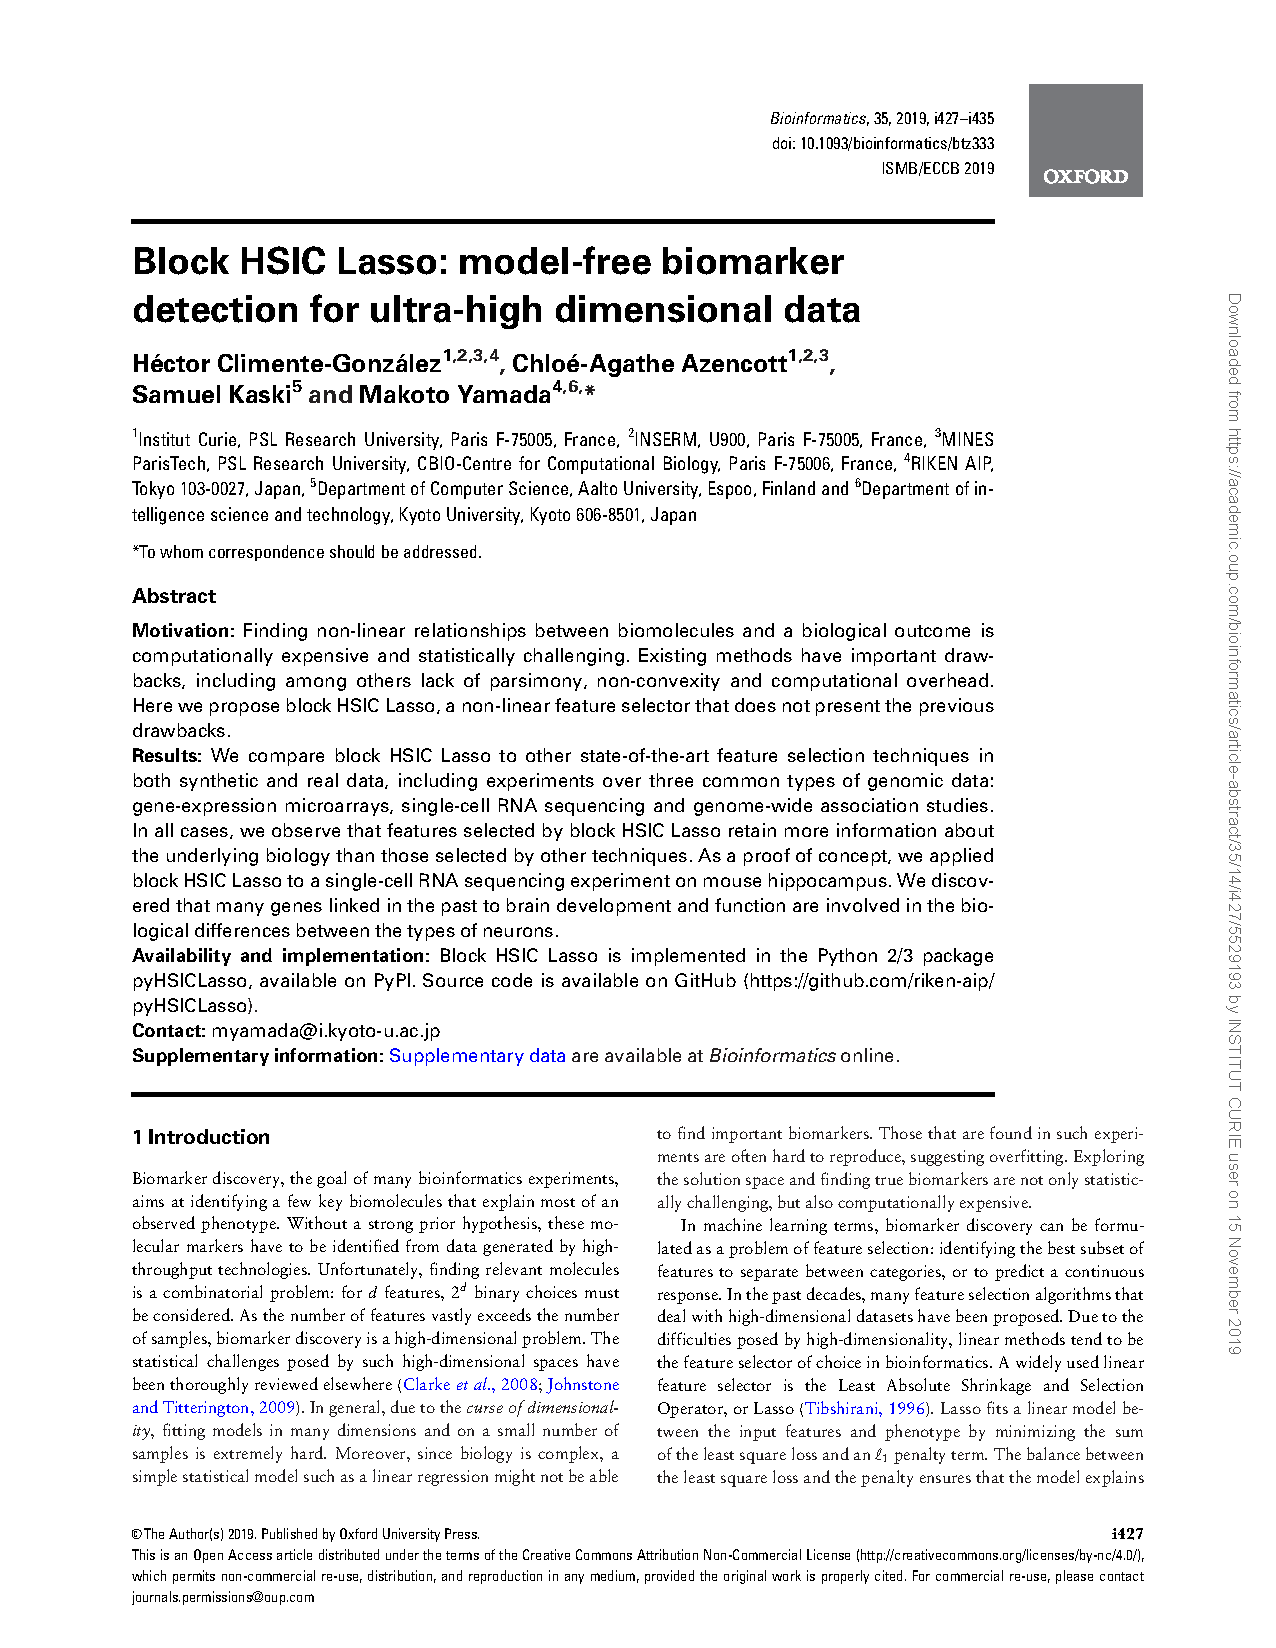
\includepdf[pages=-, scale=1]{articles/climente_2019.pdf}

\hypertarget{smartas}{%
\chapter{The Functional Impact of Alternative Splicing in Cancer}\label{smartas}}

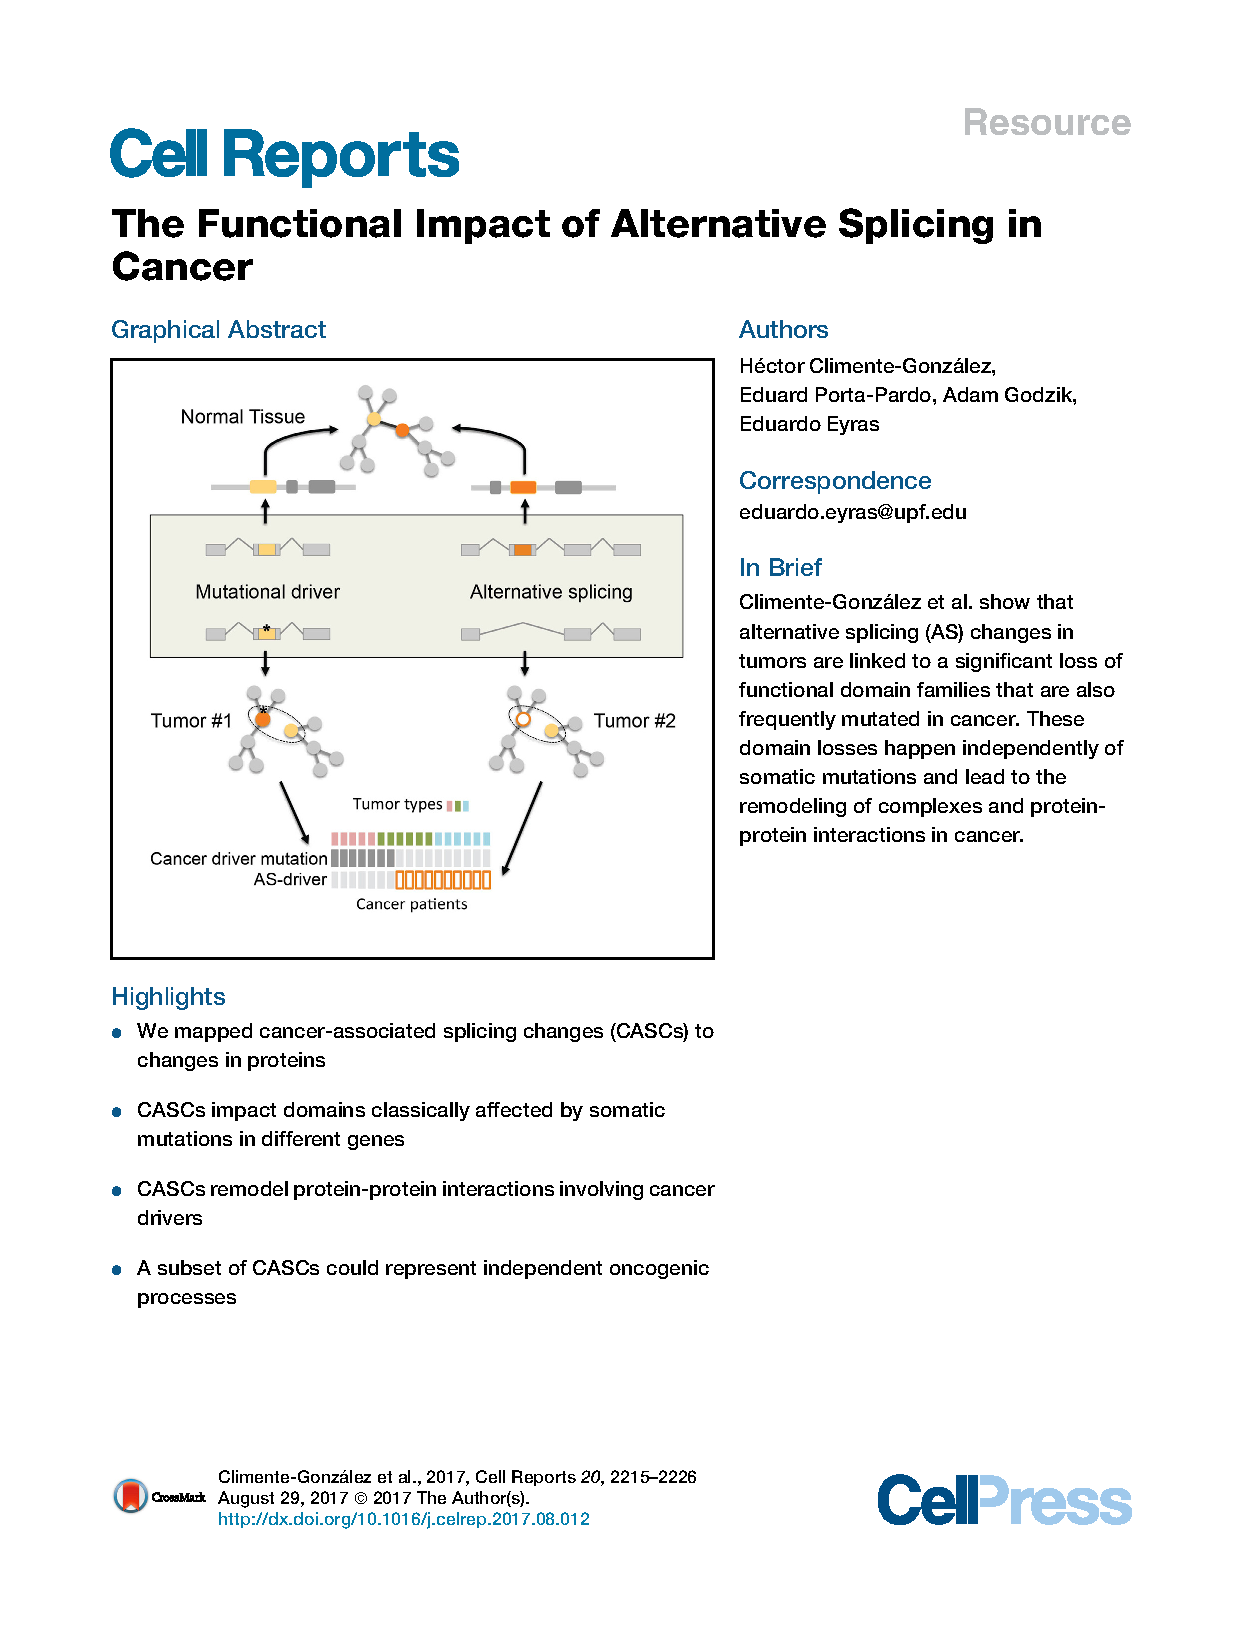
\includepdf[pages=-, scale=1]{articles/climente_2017.pdf}

\hypertarget{scm}{%
\chapter{Systematic Analysis of Splice-Site-Creating Mutations in Cancer}\label{scm}}

\includepdf[pages=-, scale=1]{articles/jayasinghe_2018.pdf}

\hypertarget{hboc-genes}{%
\chapter{Susceptibility genes to breast cancer}\label{hboc-genes}}

Nearly all known HBOC susceptibility genes encode tumor suppressors that participate in genome stability pathways (homologous recombination repair, replication fork stability, transcription-replication collisions, mismatch repair, and DNA damage signaling, checkpoints and cell death).

\hypertarget{homologous-recombination-repair}{%
\section{Homologous recombination repair}\label{homologous-recombination-repair}}

The homologous recombination repair pathway (HRR) deals with double strand DNA breaks by using the undamaged chromosome as template for error-free repair. After a DSB occurs, the MRN complex (MRE11, RAD50 and NDN) detects and binds the free DNA ends. Then, it promotes DNA damage checkpoint signaling.

HRR involves \emph{BRCA1}, \emph{BRCA2} and, actually, most of the HBOC genes. Because of its ability to interact with a wide range of proteins, BRCA1 is hypothetized to act as a recruitment scaffold. A deficiency of \emph{BRCA1} is linked to the inability to trigger HRR. Mutations in the MRN complex have also been clinically associated to breast cancer, although dubiously so in the case of \emph{RAD50} variants. Reassuringly, some other HBOC genes are interactors of the MRN complex and BRCA1/2.

\hypertarget{replication-fork-stability}{%
\section{Replication fork stability}\label{replication-fork-stability}}

BRCA1 and BRCA2 protect newly synthesized DNA and promote the restart of stalled forks in an HRR-independent manner. In the absence of these proteins, newly synthesized DNA in a stalled fork would get degraded, leading to genome instability and increasing the risk of cancer.

\hypertarget{transcription-replication-collisions}{%
\section{Transcription-replication collisions}\label{transcription-replication-collisions}}

Collisions between transcription and replication are emerging as a source of genome instability. In particular, RNA-DNA hybrids called R-loops can form between the nascent transcript and the DNA template. They can lead to double-strand breaks and mutations. Both BRCA1 and BRCA2 participate in the resolution of R-loops, preventing their accumulation. In consequence, BRCA-deficient cells tend to suffer transcriptional stress that leads to genome instability. Nonetheless the relationship between this mechanism and proneness to HBOC is yet to be proven, and the genes involved further investigated.

\hypertarget{mismatch-repair}{%
\section{Mismatch repair}\label{mismatch-repair}}

DNA mismatch repair (MMR) corrects base-base mispairs. When MMR is faulty, accumulations point mutations and genetic changes in repeated nucleotide sequences (microsatellite instability) occur. MMR also plays a role in error-free HRR.

\hypertarget{dna-damage-signaling-checkpoints-and-cell-death}{%
\section{DNA damage signaling, checkpoints and cell death}\label{dna-damage-signaling-checkpoints-and-cell-death}}

Pathways involved in genome maintenance, cell cycle checkpoints and cell death usually eliminate cells with damaged DNA. When proteins involved in them are not active, some processes such as cell cycle arrest, apoptosis and senescence will not occur. In consequence, cells that undergo genomic alterations are allowed to proliferate. The most famous case of HBOC in this pathway is TP53, which coordinates the transcriptional induction of many genome stability factors.





\begin{landscape}\begin{table}

\caption{\label{tab:hboc-genes}Overview of HBOC genes: estimated lifetime risk of breast cancer (age in years) and tumorogenic molecular mechanisms that involves them: homologous recombination repair (HRR), replication fork stability, transcription-replication collisions, mismatch repair (MMR), DNA damage signaling, checkpoints and cell death, and/or others. Adapted from Nielsen, Overeem Hansen, and Sørensen (\protect\hyperlink{ref-nielsen_hereditary_2016}{2016}).}
\centering
\begin{tabular}[t]{llllllll}
\toprule
Gene & Lifetime.risk & HRR & Rep..fork.stab. & Tr..rep..clash & MMR & DNA.Damage..apoptosis & Other\\
\midrule
\rowcolor{gray!6}  ATM & 60\% by age 80 & \(\checkmark\) &  &  &  & \(\checkmark\) & \\
BARD1 & Unknown & \(\checkmark\) &  &  &  &  & \\
\rowcolor{gray!6}  BLM & Unknown &  & \(\checkmark\) &  &  &  & \\
BRCA1 & 57-65\% by age 70 & \(\checkmark\) & \(\checkmark\) & \(\checkmark\) &  & \(\checkmark\) & \\
\rowcolor{gray!6}  BRCA2 & 45-55\% by age 70 & \(\checkmark\) & \(\checkmark\) & \(\checkmark\) &  & \(\checkmark\) & \\
\addlinespace
BRIP1 & OR: < 2.0 &  &  &  &  &  & \\
\rowcolor{gray!6}  CDH1 & 42\% by age 80 &  &  &  &  &  & \(\checkmark\)\\
CHEK2 & 37\% by age 70 &  &  &  &  & \(\checkmark\) & \\
\rowcolor{gray!6}  FAM175A & Unknown & \(\checkmark\) &  &  &  &  & \\
FANCC & Unknown &  & \(\checkmark\) &  &  &  & \\
\addlinespace
\rowcolor{gray!6}  FANCM & Unknown &  & \(\checkmark\) &  &  &  & \\
MLH1 & \textasciitilde{}19\% by age 70 &  & \(\checkmark\) &  & \(\checkmark\) &  & \\
\rowcolor{gray!6}  MRE11 & Unknown &  &  &  & \(\checkmark\) &  & \\
MSH2 & \textasciitilde{}11\% by age 70 &  &  &  & \(\checkmark\) &  & \\
\rowcolor{gray!6}  NBN & OR: 3.0 & \(\checkmark\) &  &  &  &  & \\
\addlinespace
NF1 & 6.5-fold up ages 30-39 &  &  &  &  &  & \(\checkmark\)\\
\rowcolor{gray!6}  PALB2 & 35\% by age 70 & \(\checkmark\) & \(\checkmark\) &  &  &  & \\
PMS2 & SIR: 3.8 &  &  &  & \(\checkmark\) &  & \\
\rowcolor{gray!6}  PTEN & 85\% by age 70 &  &  &  &  &  & \(\checkmark\)\\
RAD51B & Unknown & \(\checkmark\) &  &  &  &  & \\
\addlinespace
\rowcolor{gray!6}  RAD51C & Unknown & \(\checkmark\) &  &  &  &  & \\
RAD51D & Unknown & \(\checkmark\) &  &  &  &  & \\
\rowcolor{gray!6}  RECQL & Unknown &  & \(\checkmark\) &  &  &  & \\
RINT1 & Unknown & \(\checkmark\) &  &  &  &  & \\
\rowcolor{gray!6}  STK11 & 32\% by age 60 &  &  &  &  &  & \(\checkmark\)\\
\addlinespace
TP53 & 25\% by age 70 &  &  &  &  & \(\checkmark\) & \\
\bottomrule
\end{tabular}
\end{table}
\end{landscape}

\end{document}
